\documentclass{tufte-book}

%%%%%%%%%%%%%%%%%   beginning of my macros   %%%%%%%%%%%%%%%%%%%%%%%%%%%

%%%  allow chapters and sections to be numbered for tufte-book
\setcounter{secnumdepth}{1} 

%%%%%%%%%%%%%%%%%%%%%%%%%%%%%%%%%%%%%%%%%%%%%%%%%%%%%%%%%%%%%%%%%%%%%%%%
%%  Set numbering of sections, and equations
%%    (1) section number as 1, 2, 3, 4 rather than 1.1, 1.2, 2.1, 2.2
%%    (2) equation number as section.equation
%%%%%%%%%%%%%%%%%%%%%%%%%%%%%%%%%%%%%%%%%%%%%%%%%%%%%%%%%%%%%%%%%%%%%%%%
% \usepackage{remreset}
% \makeatletter \@removefromreset{section}{chapter}
% \renewcommand{\thechapter}{\@Roman\c@chapter}  % chapter number in Roman
% \renewcommand{\thesection}{\@arabic\c@section} % section number in arabic
% \makeatletter \@removefromreset{equation}{chapter}
% \@addtoreset{equation}{section}
% \renewcommand\theequation{\thesection.\arabic{equation}}
% \@addtoreset{figure}{section}
% \renewcommand\thefigure{\thesection.\arabic{figure}}
% \makeatother

%%%%%%%%%%%%%%%%%%%%%%%%%%%%%%%%%%%%%%%%%%%%%%%%%%%%%%%%%%%%%%%%%%%%%
%%   Use amsmath for equations
%%   theorems, lemma, definitions, corollary, remarks number together
%%%%%%%%%%%%%%%%%%%%%%%%%%%%%%%%%%%%%%%%%%%%%%%%%%%%%%%%%%%%%%%%%%%%%
\usepackage{amsmath,amsthm,amssymb,latexsym}
\theoremstyle{plain}
%\newtheorem{theorem}{Theorem}[section]
\newtheorem{theorem}{Theorem}[chapter] % labelled as chapter.theorem 
\newtheorem{lemma}[theorem]{Lemma}
\newtheorem{definition}[theorem]{Definition}
\newtheorem{corollary}[theorem]{Corollary}
\newtheorem{proposition}[theorem]{Proposition}
\newtheorem{example}[theorem]{Examples}
\theoremstyle{remark}
\newtheorem{remark}[theorem]{Remark}

%%%%%%%%%%%%%%%%%%%%%%%%%%%%%%%%%%%%%%%%%%%%%%
%%  declare new mathematical operators
%%%%%%%%%%%%%%%%%%%%%%%%%%%%%%%%%%%%%%%%%%%%%%
\DeclareMathOperator*\erfc {erfc}
\DeclareMathOperator*\erf {erf}

\usepackage{manfnt}   %%%  dangerous bend

%%%%%%%%%%%%%%%%%%%%%%%   end of my macros   %%%%%%%%%%%%%%%%%%%%%%%%%%%



\hypersetup{colorlinks}% uncomment this line if you prefer colored hyperlinks (e.g., for onscreen viewing)

%%
% Book metadata
%\title{A Tufte-Style Book\thanks{Thanks to Edward R.~Tufte for his inspiration.}}
%\author[The Tufte-LaTeX Developers]{The Tufte-LaTeX\ Developers}
%\publisher{Publisher of This Book}

%\title{Short Rate Models}
\title{Mathematical Notes}
\author{Pengcheng Song}
\publisher{Publisher of This Book}

%%
% If they're installed, use Bergamo and Chantilly from www.fontsite.com.
% They're clones of Bembo and Gill Sans, respectively.
%\IfFileExists{bergamo.sty}{\usepackage[osf]{bergamo}}{}% Bembo
%\IfFileExists{chantill.sty}{\usepackage{chantill}}{}% Gill Sans

%\usepackage{microtype}

%%
% Just some sample text
\usepackage{lipsum}

%%
% For nicely typeset tabular material
\usepackage{booktabs}

%%
% For graphics / images
\usepackage{graphicx}
\setkeys{Gin}{width=\linewidth,totalheight=\textheight,keepaspectratio}
\graphicspath{{graphics/}}

% The fancyvrb package lets us customize the formatting of verbatim
% environments.  We use a slightly smaller font.
\usepackage{fancyvrb}
\fvset{fontsize=\normalsize}

%%
% Prints argument within hanging parentheses (i.e., parentheses that take
% up no horizontal space).  Useful in tabular environments.
\newcommand{\hangp}[1]{\makebox[0pt][r]{(}#1\makebox[0pt][l]{)}}

%%
% Prints an asterisk that takes up no horizontal space.
% Useful in tabular environments.
\newcommand{\hangstar}{\makebox[0pt][l]{*}}

%%
% Prints a trailing space in a smart way.
\usepackage{xspace}

%%
% Some shortcuts for Tufte's book titles.  The lowercase commands will
% produce the initials of the book title in italics.  The all-caps commands
% will print out the full title of the book in italics.
\newcommand{\vdqi}{\textit{VDQI}\xspace}
\newcommand{\ei}{\textit{EI}\xspace}
\newcommand{\ve}{\textit{VE}\xspace}
\newcommand{\be}{\textit{BE}\xspace}
\newcommand{\VDQI}{\textit{The Visual Display of Quantitative Information}\xspace}
\newcommand{\EI}{\textit{Envisioning Information}\xspace}
\newcommand{\VE}{\textit{Visual Explanations}\xspace}
\newcommand{\BE}{\textit{Beautiful Evidence}\xspace}

\newcommand{\TL}{Tufte-\LaTeX\xspace}

% Prints the month name (e.g., January) and the year (e.g., 2008)
\newcommand{\monthyear}{%
  \ifcase\month\or January\or February\or March\or April\or May\or June\or
  July\or August\or September\or October\or November\or
  December\fi\space\number\year
}


% Prints an epigraph and speaker in sans serif, all-caps type.
\newcommand{\openepigraph}[2]{%
  %\sffamily\fontsize{14}{16}\selectfont
  \begin{fullwidth}
  \sffamily\large
  \begin{doublespace}
  \noindent\allcaps{#1}\\% epigraph
  \noindent\allcaps{#2}% author
  \end{doublespace}
  \end{fullwidth}
}

% Inserts a blank page
\newcommand{\blankpage}{\newpage\hbox{}\thispagestyle{empty}\newpage}

\usepackage{units}

% Typesets the font size, leading, and measure in the form of 10/12x26 pc.
\newcommand{\measure}[3]{#1/#2$\times$\unit[#3]{pc}}

% Macros for typesetting the documentation
\newcommand{\hlred}[1]{\textcolor{Maroon}{#1}}% prints in red
\newcommand{\hangleft}[1]{\makebox[0pt][r]{#1}}
\newcommand{\hairsp}{\hspace{1pt}}% hair space
\newcommand{\hquad}{\hskip0.5em\relax}% half quad space
\newcommand{\TODO}{\textcolor{red}{\bf TODO!}\xspace}
\newcommand{\ie}{\textit{i.\hairsp{}e.}\xspace}
\newcommand{\eg}{\textit{e.\hairsp{}g.}\xspace}
\newcommand{\na}{\quad--}% used in tables for N/A cells
\providecommand{\XeLaTeX}{X\lower.5ex\hbox{\kern-0.15em\reflectbox{E}}\kern-0.1em\LaTeX}
\newcommand{\tXeLaTeX}{\XeLaTeX\index{XeLaTeX@\protect\XeLaTeX}}
% \index{\texttt{\textbackslash xyz}@\hangleft{\texttt{\textbackslash}}\texttt{xyz}}
\newcommand{\tuftebs}{\symbol{'134}}% a backslash in tt type in OT1/T1
\newcommand{\doccmdnoindex}[2][]{\texttt{\tuftebs#2}}% command name -- adds backslash automatically (and doesn't add cmd to the index)
\newcommand{\doccmddef}[2][]{%
  \hlred{\texttt{\tuftebs#2}}\label{cmd:#2}%
  \ifthenelse{\isempty{#1}}%
    {% add the command to the index
      \index{#2 command@\protect\hangleft{\texttt{\tuftebs}}\texttt{#2}}% command name
    }%
    {% add the command and package to the index
      \index{#2 command@\protect\hangleft{\texttt{\tuftebs}}\texttt{#2} (\texttt{#1} package)}% command name
      \index{#1 package@\texttt{#1} package}\index{packages!#1@\texttt{#1}}% package name
    }%
}% command name -- adds backslash automatically
\newcommand{\doccmd}[2][]{%
  \texttt{\tuftebs#2}%
  \ifthenelse{\isempty{#1}}%
    {% add the command to the index
      \index{#2 command@\protect\hangleft{\texttt{\tuftebs}}\texttt{#2}}% command name
    }%
    {% add the command and package to the index
      \index{#2 command@\protect\hangleft{\texttt{\tuftebs}}\texttt{#2} (\texttt{#1} package)}% command name
      \index{#1 package@\texttt{#1} package}\index{packages!#1@\texttt{#1}}% package name
    }%
}% command name -- adds backslash automatically
\newcommand{\docopt}[1]{\ensuremath{\langle}\textrm{\textit{#1}}\ensuremath{\rangle}}% optional command argument
\newcommand{\docarg}[1]{\textrm{\textit{#1}}}% (required) command argument
\newenvironment{docspec}{\begin{quotation}\ttfamily\parskip0pt\parindent0pt\ignorespaces}{\end{quotation}}% command specification environment
\newcommand{\docenv}[1]{\texttt{#1}\index{#1 environment@\texttt{#1} environment}\index{environments!#1@\texttt{#1}}}% environment name
\newcommand{\docenvdef}[1]{\hlred{\texttt{#1}}\label{env:#1}\index{#1 environment@\texttt{#1} environment}\index{environments!#1@\texttt{#1}}}% environment name
\newcommand{\docpkg}[1]{\texttt{#1}\index{#1 package@\texttt{#1} package}\index{packages!#1@\texttt{#1}}}% package name
\newcommand{\doccls}[1]{\texttt{#1}}% document class name
\newcommand{\docclsopt}[1]{\texttt{#1}\index{#1 class option@\texttt{#1} class option}\index{class options!#1@\texttt{#1}}}% document class option name
\newcommand{\docclsoptdef}[1]{\hlred{\texttt{#1}}\label{clsopt:#1}\index{#1 class option@\texttt{#1} class option}\index{class options!#1@\texttt{#1}}}% document class option name defined
\newcommand{\docmsg}[2]{\bigskip\begin{fullwidth}\noindent\ttfamily#1\end{fullwidth}\medskip\par\noindent#2}
\newcommand{\docfilehook}[2]{\texttt{#1}\index{file hooks!#2}\index{#1@\texttt{#1}}}
\newcommand{\doccounter}[1]{\texttt{#1}\index{#1 counter@\texttt{#1} counter}}




%%%%%%%%%%%%%%%%%%%%%%%%%%%%%%%%%%%%%%%%
%%%  beginning of my own code 
\usepackage{tikz}  
\usetikzlibrary{arrows,snakes}  

%% New command for drawing snake line.
%% e.g.  \drawsnake{(0,0)}{(0,2){$y=\sigma$}
%% draws a snake line from (0,0) to (0,2) with text $y=\sigma$
\newcommand{\drawsnake}[3]
{
  \draw [->, >=triangle 90,decorate,decoration={snake,amplitude=1mm,segment length=6mm,post
        length=1mm, pre length=1mm}]  #1 -- #2 
  node[above,text centered]{ #3 };
}

\newcommand{\drawbreakright}[2]
{
  \draw (#1,#2) -- (#1,#2+0.2) -- (#1+0.2,#2-0.2) -- (#1+0.2,#2);
}

\newcommand{\drawbreakleft}[2]
{
  \draw (#1,#2) -- (#1,#2-0.2) -- (#1-0.2,#2+0.2) -- (#1-0.2,#2);
}
%%%  end of my own code  %%%
%%%%%%%%%%%%%%%%%%%%%%%%%%%%%%%%%%%%%%%%





% Generates the index
\usepackage{makeidx}
\makeindex



%%%%%%%%%%%%%%%%%%%%%%%%%%%%%%%%%%%%%
\begin{document}


% Front matter
\frontmatter

% % r.1 blank page
% \blankpage
% 
% % v.2 epigraphs
% \newpage\thispagestyle{empty}
% \openepigraph{%
% The public is more familiar with bad design than good design.
% It is, in effect, conditioned to prefer bad design, 
% because that is what it lives with. 
% The new becomes threatening, the old reassuring.
% }{Paul Rand%, {\itshape Design, Form, and Chaos}
% }
% \vfill
% \openepigraph{%
% A designer knows that he has achieved perfection 
% not when there is nothing left to add, 
% but when there is nothing left to take away.
% }{Antoine de Saint-Exup\'{e}ry}
% \vfill
% \openepigraph{%
% \ldots the designer of a new system must not only be the implementor and the first 
% large-scale user; the designer should also write the first user manual\ldots 
% If I had not participated fully in all these activities, 
% literally hundreds of improvements would never have been made, 
% because I would never have thought of them or perceived 
% why they were important.
% }{Donald E. Knuth}


% r.3 full title page
\maketitle


% v.4 copyright page
% \newpage
% \begin{fullwidth}
% ~\vfill
% \thispagestyle{empty}
% \setlength{\parindent}{0pt}
% \setlength{\parskip}{\baselineskip}
% Copyright \copyright\ \the\year\ \thanklessauthor
% 
% \par\smallcaps{Published by \thanklesspublisher}
% 
% \par\smallcaps{tufte-latex.googlecode.com}
% 
% \par Licensed under the Apache License, Version 2.0 (the ``License''); you may not
% use this file except in compliance with the License. You may obtain a copy
% of the License at \url{http://www.apache.org/licenses/LICENSE-2.0}. Unless
% required by applicable law or agreed to in writing, software distributed
% under the License is distributed on an \smallcaps{``AS IS'' BASIS, WITHOUT
% WARRANTIES OR CONDITIONS OF ANY KIND}, either express or implied. See the
% License for the specific language governing permissions and limitations
% under the License.\index{license}
% 
% \par\textit{First printing, \monthyear}
% \end{fullwidth}

% r.5 contents
\tableofcontents

% \listoffigures

% \listoftables

% r.7 dedication
% \cleardoublepage
% ~\vfill
% \begin{doublespace}
% \noindent\fontsize{18}{22}\selectfont\itshape
% \nohyphenation
% Dedicated to those who appreciate \LaTeX{} 
% and the work of \mbox{Edward R.~Tufte} 
% and \mbox{Donald E.~Knuth}.
% \end{doublespace}
% \vfill
% \vfill


% r.9 introduction
% \cleardoublepage
% \chapter*{Introduction}
% 
% This sample book discusses the design of Edward Tufte's
% books\cite{Tufte2001,Tufte1990,Tufte1997,Tufte2006}
% and the use of the \doccls{tufte-book} and \doccls{tufte-handout} document classes.


%%%%%%%%%%%%%%%%%%%%%%%%%%%%%%%%%%%%%%%%%%%%%%%%
%%    Start the main matter (normal chapters)
%%%%%%%%%%%%%%%%%%%%%%%%%%%%%%%%%%%%%%%%%%%%%%%%
\mainmatter

\chapter{Single-period Option Pricing}

In this chapter we lay out the foundation of option pricing under discrete
setting.
We mostly follow Chapter 1, Single-period Option Pricing of Hunt and Kennedy's
Financial Derivatives in Theory and Practice, revised edition.

We consider an economy $\mathcal{E}$ comprising $n$ assets with $m$ possible
states at time $1$. Let $\Omega$ be the set of all possible states. We denote
the individual states by $w_j,j=1,2,\cdots,m$, and the $i$-th asset price at 
time $0$ by $A_0^{(i)}$ and at state $w_j$ at time $1$ by $A_1^{(i)}(w_j)$.
We define matrix $(A_1)_{n\times m}$ as
\begin{equation}
  (A_1)_{n\times m} = 
    \begin{pmatrix}
      A_1^{(1)}(w_1) & A_1^{(1)}(w_2) & \cdots & A_1^{(1)}(w_m) \\
      A_1^{(2)}(w_1) & A_1^{(2)}(w_2) & \cdots & A_1^{(2)}(w_m) \\
      \vdots         & \vdots         & \ddots & \vdots         \\
      A_1^{(n)}(w_1) & A_1^{(n)}(w_2) & \cdots & A_1^{(n)}(w_m) \\
    \end{pmatrix}
\end{equation}

%%%%%%%%%%%%%%%%%%%%%%%%%%
\begin{definition}
The economy $\mathcal{E}$ admits $\mathbf{arbitrage}$ if there exists a 
portfolio $\phi\in R^n$ such that one of the following conditions holds:
\begin{enumerate}
  \item[(1)] $\phi\cdot A_0<0$, and $\phi\cdot A_1(w_j)\ge 0$ for all $j$.
  \item[(2)] $\phi\cdot A_0\le 0$, and $\phi\cdot A_1(w_j)\ge 0$ for all $j$,
    with strict inequality for some $j$.
  \item[(3)] $\phi\cdot A_0=0$, and $\phi\cdot A_1(w_j)\ge 0$ for all $j$,
    with strict inequality for some $j$.
\end{enumerate}
\end{definition}

%%%%%%%%%%%%%%%%%%%%%%%%%%
\begin{proposition}
The three conditions in the defintion of arbitrage are equivalent.
\end{proposition}
\begin{proof}
TODO. May need a numeraire.
\end{proof}

%%%%%%%%%%%%%%%%%%%%%%%%%%
\begin{definition}
A derivative $X$ is said to be $\mathbf{attainable}$ if there exists some 
$\phi\in R^n$ such that for all $j=1,2,\cdots,m$
\begin{equation}
  X_1(w_j) = \phi\cdot A_1(w_j).
\end{equation}
where $X_1(w_j)$ is the price of $X$ at time $1$ if the state is $w_j$.
Or in matrix form $X_1=A_1^T \phi$.
\end{definition}

%%%%%%%%%%%%%%%%%%%%%%%%%%
\begin{definition}
A pricing kernel $Z\in R^m$ is any strictly positive vector with the
property
\footnote{Alternatively pricing kernel can be defined as the Arrow-Debreu 
  price, i.e. $Z_j$ is the time $0$ price of an instrument that pays $\$1$
  if it is in state $w_j$ at time $1$ and pays nothing otherwise.}
\begin{equation}
  A_0 = \sum_{j=1}^m Z_j A_1(w_j) = A_1 Z.
\end{equation}
\end{definition}


%%%%%%%%%%%%%%%%%%%%%%%%%%
\section{Pricing}

%%%%%%%%%%%%%%%%%%%%%%%%%%
\begin{theorem} \label{T:price}
\footnote{Hunt and Kennedy, Financial Derivatives in Theory and Practice, 
    revised edition, Theorem 1.4, pp.6-7}
Suppose that the economy $\mathcal{E}$ is arbitrage-free and let $X$ be an
attainable contingent claim, i.e., a derivative which can be replicated with
other assets. Then the fair value of $X$ is given by 
\begin{equation}
  X_0 = \phi\cdot A_0,
\end{equation}
where $\phi$ solves for $j=1,2,\cdots,m$
\[
  X_1(w_j) = \phi\cdot A_1(w_j).
\]
Furthermore, if $Z$ is some pricing kernel for the economy then $X_0$ can also
be represented as
\[
  X_0 = \sum_j Z_j X_1(w_j).
\]
\end{theorem}
\begin{proof}
The first part follows by the following arbitrage argument. 
If $X_0>\phi\cdot A_0$, then
the portfolio of $\phi$ minus one unit of $X$ would have negative value at time
$0$ but value zero at all states of time $1$, hence would admit an arbitrage.
Similarly if $X_0>\phi\cdot A_0$ there would also exist an arbitrage. Since the
economy is arbitrage-free, the equality follows.

The second part is valid because
\[
  X_0=\phi\cdot A_0 = \sum_j Z_j (\phi\cdot A_1(w_j)) = \sum_j Z_j X_1(w_j).
\]
\end{proof}


%%%%%%%%%%%%%%%%%%%%%%%%%%
\section{Condition for No-arbitrage: Existence of Pricing Kernel}

%%%%%%%%%%%%%%%%%%%%%%%%%%
\begin{theorem} \label{T:no_arb}
\footnote{Hunt and Kennedy, Financial Derivatives in Theory and Practice, 
    revised edition, Theorem 1.7, pp. 7-9. This is similar to Farkas's 
    Lemma \ref{T:farkas}.}
The economy $\mathcal{E}$ is arbitrage-free iff there exists a pricing kernel,
i.e., a strictly positive $Z$ such that
\[
  A_0 = \sum_j Z_j A_1(w_j).
\]
\end{theorem}
\begin{proof} %%%%%%%%%%%%%%%%%%%%%%%%%%%%%%%%%%%%%%%%%%%%%%%%%%%%%
Suppose there exist a pricing kernel $Z$, then for any $\phi$ such that 
$\phi\cdot A_0<0$ we have
\[
  \phi\cdot A_0 = \sum_j Z_j (\phi\cdot A_1(w_j)) < 0,
\]
since $Z_j>0$ for all $j$, there exists a $k$ such that $\phi\cdot A_1(w_k)<0$,
hence there is no arbitrage.

%To verify the converse, we need the separating hyperplane theorem.
%\footnote{Precise statement? Proof? Elliott and Kopp, Mathematics of Finance,
%    2nd ed., section 3.1, pp.57-59}
%TODO
Conversely, suppose no such $Z$ exists, we will construct an arbitrage
portfolio. Let $C$ be the convex cone constructed from $A_1(\cdot)$,
\[
  C = \{a: a=\sum_j Z_j A_1(w_j), Z>0  \}.
\]
The set $C$ is a non-empty convex set not containing $A_0$, hence by the
separating hyperplane theorem \ref{T:sep_plane}
%\footnote{Precise statement? Proof? Elliott and Kopp, Mathematics of Finance,
%    2nd ed., section 3.1, pp.57-59}
there exists a hyperplane $H=\{x:\phi\cdot x=\beta\}$ that separates $A_0$ and
$C$,
\[
  \phi\cdot A_0 \leq \beta \leq \phi\cdot a, \qquad \forall a\in C.
\]
The vector $\phi$ represents an arbitrage portfolio, as we now demonstrate.

First observe that if $a\in\bar{C}$ (the closure of $C$) then for any 
$\mu\geq 0$ we have $\mu a\in\bar{C}$, and 
\[
  \beta\leq \mu(\phi\cdot a).
\]
Taking $\mu=0$ yields $\phi\cdot A_0\leq \beta\leq 0$. Letting
$\mu\uparrow\infty$ shows that $\phi\cdot a\geq 0$ for all $a\in \bar{C}$, in
particular $\phi\cdot A_1(w_j)\geq 0$ for all $j$. So we have
\[
  \phi\cdot A_0\leq 0 \leq \phi\cdot A_1(w_j), \qquad \forall j,
\]
and it only remains to show that this is not always identically zero. but in
this case $\phi\cdot A_0=\phi\cdot C=0$ which violates the separating property
for $H$.
\end{proof} %%%%%%%%%%%%%%%%%%%%%%%%%%%%%%%%%%%%%%%%%%%%%%%%%%%%%%%%%%

%%%%%%%%%%%%%%%%%%%%%%%%%%
\section{Completeness: Uniqueness of Pricing Kernel}

%%%%%%%%%%%%%%%%%%%%%%%%%%%%%%%%%%%%%%%
\begin{theorem}[Rank-nullity Theorem] \label{T:rank}
Let $V$ and $W$ be two vector spaces and let $T:V\to W$ be a linear map. The
kernel of $T$ is defined as
\[
  ker T = \{v\in V: T(v)=0 \}.
\]
The dimension of the image of $T$ is called the rank, and the dimension of the
kernel is called the nullity. And we have
\[
  dim(im T) + dim(ker T) = dim V.
\]
\end{theorem}
\begin{proof}  %%%%%%%%%%%%%%%%%%%%%%%%%%%%%
Here we prove the theorem in the finite-dimensional case.
\footnote{Adapted from Wikipedia
    (http://en.wikipedia.org/wiki/Rank-nullity\_theorem) and
    MacLean and Birkhoff, Algebra, 3rd ed., VI.3, Theorem 8, pp. 202-203.
    A more general proof which also covers infinite dimensional case is in
    Roman, Advanced Linear Algebra, 3rd ed., Theorem 2.8, p.63}
Suppose $\{u_1,\cdots,u_m\}$ forms a basis of $ker T$. We can extend this to 
form a basis of $V$: $\{u_1,\cdots,u_m,w_1,\cdots,w_n\}$. Since the dimension
of $ker T$ is $m$ and the dimension of $V$ is $m+n$, it suffices to show that
the dimension of $im T$ is $n$.

Since any vector $v\in V$ is a linear combination
\[
  v = \sum_{i=1}^m a_i u_i + \sum_{j=1}^n b_j w_j,
\]
for suitable lists $a$ and $b$ of scalars, and since $Tu_i=0$ for 
$i=1,\cdots,m$, we get
\[
  Tv = \sum_{j=1}^n b_j Tw_j,
\]
i.e. the list $\{Tw_1,\cdots,Tw_n\}$ spans $im T$. For this to be a basis, we
only need to verify that it is linearly independent. Note that 
$\sum_{j=1}^n c_j (Tw_j)=0$ means that $T(\sum_{j=1}^n c_j w_j)=0$, i.e. 
$\sum_{j=1}^n c_j w_j\in ker T$, hence
\[
  \sum_{j=1}^n c_j w_j = \sum_{i=1}^m d_i u_i,
\]
and since $\{u_1,\cdots,u_m,w_1,\cdots,w_n\}$ is linearly independent,
all $c_j$ and $d_i$ must be zero, hence the list $\{Tw_1,\cdots,Tw_n\}$ 
is linearly independent in $im T$, and thus a basis, as asserted.
\end{proof}  %%%%%%%%%%%%%%%%%%%%%%%%%%%%%

%%%%%%%%%%%%%%%%%%%%%%%%%%%%%%%%%%%%%%%
\begin{theorem} \label{T:comp}
\footnote{Hunt and Kennedy, Financial Derivatives in Theory and Practice, 
    revised edition, Theorem 1.9, p.10}
The economy $\mathcal{E}$ is complete iff there exists a (generalized) left
inverse $A^{-1}$ for the matrix $A$
\[
  A_{ij} = A_1^{(i)}(w_j), \qquad i=1,2,\cdots,n, \, j=1,2,\cdots,m.
\]
Equivalently, $\mathcal{E}$ is complete iff there exists no non-zero solution to
the equation $Ax=0$.
\end{theorem}
\begin{proof}
For the economy to be complete, given any contingent claim $X$, we must be able
to solve $\phi$ such that
\[
  X_1(w_j) = \phi\cdot A_1(w_j), \qquad j=1,2,\cdots,m
\]
which can be written as a matrix equation
\footnote{ \textdbend $(X_1)_{m\times 1} = (A^T)_{m\times n} (\phi)_{n\times 1}$.
          We can not simply solve this equation by multiplying both sides
          by the left inverse of $A^T$ because it does not necessarily
          exist, even in the case of $m=n$. Think about it!}
\[
  X_1 = A^T \phi.
\]
For this equation to have a solution for any $X_1$, it is necessary and
sufficient that the equation to have a solution for $m$ vectors 
$(1,0,\cdots,0)^T$, $(0,1,0,\cdots,0)^T$,etc,$(0,0,\cdots,0,1)^T$ each of 
size $m$, i.e. the standard basis of vector space $R^m$.
Let the solutions be $b_1,b_2,\dots,b_m$, each of size $n\times 1$, and
let $B$ be a $n\times m$ matrix made up of column vectors
$b_1,b_2,\dots,b_m$, then $A^T B=I_m$, i.e. $B$ is a right inverse of $A^T$.
%This is equivalent to the condition that 
%$A^T$ has a right inverse, i.e. there exists a $n\times m$
%matrix $B$ such that $A^T B= I$, where $I$ is the $m\times m$ identity matrix.
And this in turn is equivalent to the condition that $A$ has a left inverse 
since
\[
  I_m = (A^T B)^T = B^T A.
\]

% Next we verify that $A$ has a left inverse is equivalent to the condition that
% equation $Ax=0$ only has zero solution. First note that if $A$ has a left
% inverse, then for any vector $x$ satisfying $Ax=0$ we have
% \[
%   A^{-1} (Ax) = x = 0.
% \]

%To verify the converse, note that if $x\neq 0$ and $Ax=0$, then equation
%$x=A^T \phi$ does not have a solution because for any $\phi$
%\[
%  0 = (\phi^T (Ax) )^T = x^T (A^T \phi),
%\]
%but $x^T x\neq 0$. Hence $A^T$ does not have a right inverse, thus $A$ does not
%have a left inverse.

%To verifty the converse, suppose $A$ does not have a left inverse, thus $A^T$
%does not have a right inverse, hence there exists a $n\times 1$ vector 
%$x\neq 0$ such that for all $\phi$ we have $x\neq A^T \phi$. This implies that 
%equation
%\[
%  a x = \sum_i b_i (A^T \phi)_i
%\]
%only has zero solution $a=b_1=b_2=\cdots=0$, where $\{(A^T \phi)_i\}_i$ is the 
%basis of linear space $A^T \phi$. The same conclusion applies to equation
%\[
%  a (x^T x) = \sum_i b_i (x^T (A^T \phi)_i).
%\]
%Thus for all $\phi$ we have
%\[
%  x^T (A^T \phi) =0.
%\]
%Hence $Ax=0$ because for all $\phi$ 
%\[
%  0 = (x^T (A^T \phi))^T = \phi^T (Ax).
%\]

%To verify the converse, suppose there exists a vector $x\neq 0$ such that
%$Ax=0$. Suppose that there exists a vector $\phi$ such that $A^T \phi=x$,
%\[
%  x^T x= (A^T \phi)^T x = \phi^T (Ax) = 0,
%\]
%this is in conflict with the assumption $x\neq 0$, hence there is no solution
%for equation $x=A^T \phi$. 

% To verify the converse, note that if there exists no non-zero solution to
% equation $Ax=0$, the nullity of $A$ is zero, and due to the rank-nullity
% theorem, the rank of $A$ (and $A^T$) is $m$. Let $e_1,e_2,\cdots,e_m$ be a
% basis of the column space $F^n$ of $A^T$, then $A^T e_1,A^T e_2,\cdots,A^T e_m$ 
% is a basis of the row space $F^m$ of $A^T$.
% \footnote{Roman, Advanced Linear Algebra, 3rd ed., Theorem 2.4, p.62,
% where $A^T:F^n \to F^m$ is a linear mapping.}
% Thus for any vector $y$ in $F^m$ 
% there exists $c_1,c_2,\cdots,c_m$ such that
% \[
%   y = \sum_{i=1}^m c_i A^T e_i = A^T \sum_i c_i e_i,
% \]
% i.e. there exists a vector $\phi$ in $F^n$ such that $y=A^T \phi$.

Next we verify that economy $\mathcal{E}$ is complete iff there exists no 
non-zero solution to the equation $Ax=0$. Now $\mathcal{E}$ is complete iff
$A^T:F^n\to F^m$ is surjective, i.e. $rank(A^T)=rank(A)=m$. 
\footnote{Proof of $rank(A^T)=rank(A)$ see Roman, Advanced Linear Algebra, 
          3rd ed., Theorem 1.16, p.53}
From the rank-nullity theorem \ref{T:rank}, this is equivalent to the condition
that $dim(ker A)=0$, i.e. there exists no non-zero solution to equation
$Ax=0$.
\end{proof}


%%%%%%%%%%%%%%%%%%%%%%%%
\begin{theorem} \label{T:comp2}
\footnote{Hunt and Kennedy, Financial Derivatives in Theory and Practice, 
    revised edition, Theorem 1.12, p.11}
Suppose the economy $\mathcal{E}$ is arbitrage-free. Then it is complete iff 
there exists a unique pricing kernel $Z$.
\end{theorem}
\begin{proof}
By Theorem \ref{T:no_arb} there exists some positive vector $Z$ satisfying
\begin{equation} \label{E:ker}
  A_0 = \sum_j Z_j A_1(w_j).
\end{equation}
By Theorem \ref{T:comp}, it suffices to show that $Z$ being unique is equivalent
to there being no nonzero solution to $A x=0$. If $Z_2\neq Z$ also solves
Eq. \ref{E:ker}, then $x=Z_2-Z\neq 0$ solves $Ax=0$. Conversely, if $Z$ solves
Eq. \ref{E:ker} and $x\neq 0$ solves $A x=0$, then $Z_2=Z+\epsilon x$ also solves
Eq. \ref{E:ker}, with small enough $\epsilon$ we can have a positive $Z_2$ thus a
second pricing kernel.
\end{proof}


%%%%%%%%%%%%%%%%%%%%%%%%%%
\section{Probabilistic formulation}

%%%%%%%%%%%%%%%%%%%%%%%%
\begin{definition}
A numeraire $N$ of an economy $\mathcal{E}$ is an attainable contigent claim 
(i.e. there exist a vector $\psi$ such that $N_1=\psi\cdot A_1$) that is 
strictly positive (i.e. $N_0>0$ and $P(N_1>0)=1$).
\end{definition}

%%%%%%%%%%%%%%%%%%%%%%%%
\begin{theorem} \label{T:no_arb2}
\footnote{Hunt and Kennedy, Financial Derivatives in Theory and Practice, 
    revised edition, Theorem 1.15, p.12}
The economy $\mathcal{E}$ is arbitrage-free iff there exists a strictly positive
random variable $Z$ such that
\begin{equation} \label{E:ker2}
  A_0 = E[Z A_1].
\end{equation}
We also call $Z$ a pricing kernel for the economy $\mathcal{E}$.

Suppose further that there exists a numeraire $N$ of the economy,
%\begin{equation}
%  U_0 = E[Z U_1],
%\end{equation}
then the economy $\mathcal{E}$ is arbitrage-free iff there exists a strictly 
positive random variable $k$ such that $E[k]=1$ and
\begin{equation} \label{E:ker3}
  E\left[ k \frac{A_1}{N_1} \right] = \frac{A_0}{N_0}.
\end{equation}
\end{theorem}
\begin{proof}
The first result follows immediately from Theorem \ref{T:no_arb} by setting
\[
  Z(w_j) = \frac{Z_j}{P(w_j)},
\]
because
\[
  E[Z A_1] = \sum_j P(w_j) Z(w_j) A_1(w_j).
\]

To prove the second part we show that \ref{E:ker2} and \ref{E:ker3} are
equivalent. This follows since, given either $Z$ or $k$, we can define
the other via
\[
  Z(w_j) = k(w_j) \frac{N_0}{N_1(w_j)}.
\]
It is easy to see that $E(k)=1$ if $Z$ exists because 
\[
  E(k) = E[Z N_1] / N_0 = 1.
\]
\end{proof}


%%%%%%%%%%%%%%%%%%%%%%%%%%
\begin{definition}
\footnote{Hunt and Kennedy, Financial Derivatives in Theory and Practice, 
    revised edition, Theorem 1.19, p.14}
Two probability measures $P$ and $Q$ on the finite sample space $\Omega$ are
said to be equivalent, written $P\sim Q$, if 
\[
  P(F)=0 \Leftrightarrow Q(F)=0,
\]
for all $F\subset Q$. If $P\sim Q$ we can define the Radon-Nikodym derivative of
$P$ with respect to $Q$, $\frac{dP}{dQ}$, by
\[
  \frac{dP}{dQ}(S) = \frac{P(S)}{Q(S)}.
\]
\end{definition}

%%%%%%%%%%%%%%%%%%%%%%%%
\begin{theorem} \label{T:emm}
\footnote{Hunt and Kennedy, Financial Derivatives in Theory and Practice, 
    revised edition, Theorem 1.20, p.14}
Let $N$ be a numeraire of economy $\mathcal{E}$, then $\mathcal{E}$ is 
arbitrage-free iff there exists a probability measure $Q$ equivalent to $P$ such
that
\begin{equation} \label{E:emm}
  E_Q\left[ \frac{A_1}{N_1}  \right] = \frac{A_0}{N_0}.
\end{equation}
The measure $Q$ is called an equivalent martingale measure (EMM) for $N$.
\end{theorem}
%%%%%%%%%%%%%%%%
\begin{proof}
By Theorem \ref{T:no_arb2} we must show that Equation \ref{E:emm} is equivalent
to the existence of a strictly positive random variable $k$ with $E(k)=1$ such
that
\[
  E\left[ k \frac{A_1}{N_1} \right] = \frac{A_0}{N_0}.
\]
Suppose $\mathcal{E}$ is arbitrage-free and such $k$ exists. Define $Q\sim P$ by
$Q(w_j)=k(w_j) P(w_j)$. Then
\[
  E_Q \left[ \frac{A_1}{N_1} \right] 
  =  E\left[ \frac{dQ}{dP} \frac{A_1}{N_1} \right] 
  =  E\left[ k \frac{A_1}{N_1} \right] 
  = \frac{A_0}{N_0},
\]
as required.

Conversely, if Equation \ref{E:emm} holds then define $k(w_j)=Q(w_j)/ P(w_j)$. 
It follows easily that $E[k]=1$. Furthermore,
\[
  E\left[ k \frac{A_1}{N_1} \right] 
  =  E\left[ \frac{dQ}{dP} \frac{A_1}{N_1} \right] 
  = E_Q \left[ \frac{A_1}{N_1} \right] 
  = \frac{A_0}{N_0},
\]
and there is no arbitrage by Theorem \ref{T:no_arb2}.
\end{proof}

%%%%%%%%%%%%%%%%%%%%%%%%
\begin{theorem}
\footnote{Hunt and Kennedy, Financial Derivatives in Theory and Practice, 
    revised edition, Theorem 1.21, p.15}
Let $N$ be a numeraire of an arbitrary free economy $\mathcal{E}$, then 
$\mathcal{E}$ is complete iff there exists a unique equivalent martingale
measure for numeraire $N$.
\end{theorem}  
\begin{proof}
Observe that in the proof of Theorem \ref{T:emm} we established a one-to-one
correspondence between pricing kernels and equivalent martingale measures. The
result now follows from Theorem \ref{T:comp2} which establishes the equivalence
of completeness to the existence of a unique pricing kernel.
\end{proof}

%%%%%%%%%%%%%%%%%%%%%%%%
\begin{theorem}
\footnote{Hunt and Kennedy, Financial Derivatives in Theory and Practice, 
    revised edition, Theorem 1.22, p.15}
Suppose $\mathcal{E}$ is arbitrage-free and $N$ is a numeraire, and that $X$ is
an attainable contingent claim. Then the fair value of $X$ is given by 
\[
  X_0 = N_0 E_Q[X_1 / N_1],
\]
where $Q$ is an equivalent martingale measure for numeraire $N$.
\end{theorem}  
\begin{proof}  %%%%%%%%%%%%%%%%%%%%%%%%%%%%%%%%%%%%%%%%%%%%%%%%%%%
From Theorem \ref{T:emm} we know that
\[
  E_Q\left[ \frac{A_1}{N_1}  \right] = \frac{A_0}{N_0}.
\]
Now since $X$ is attainable, there exists a vector $\phi$ such that 
$X_1=\phi\cdot A_1$, hence
\[
  E_Q\left[ \frac{\phi\cdot A_1}{N_1}  \right] = \frac{\phi\cdot A_0}{N_0},
\]
Now since $\mathcal{E}$ is arbitrage-free, from Theorem \ref{T:price} we have
$X_0 = \phi\cdot A_0$ and hence
\[
  E_Q\left[ \frac{X_1}{N_1}  \right] = \frac{X_0}{N_0}.
\]
\end{proof}    %%%%%%%%%%%%%%%%%%%%%%%%%%%%%%%%%%%%%%%%%%%%%%%%

%%%%%%%%%%%%%%%%%%%%%%%%%%%%
\begin{remark} \label{R:radon_num}
Let $N,S$ be two numeraires and $T>t$, then we have
\[
	V_t = N_t \cdot E_N\left[ \frac{V_T}{N_T} \bigg| \mathcal{F}_t \right]
    	= S_t \cdot E_S\left[ \frac{V_T}{S_T} \bigg| \mathcal{F}_t \right]
			= S_t \cdot E_N\left[ \frac{dQ^S}{dQ^N} \frac{V_T}{S_T} \bigg|
     			\mathcal{F}_t \right]
\]
thus the Radon-Nikodym derivative between the two measures using $S$ and $N$
as numeraires is
\[
	\frac{dQ^S}{dQ^N} = \frac{S_T/S_t}{N_T/N_t}.
\]
\end{remark}
  % single period option pricing
\chapter{Convex Sets}

%%%%%%%%%%%%%%%%%%%%%%%%%%%%%%%%%%%
\section{Separating Hyperplane}

%%%%%%%%%%%%%%%%%%%
\begin{definition}
A hyperplane $H(a,\alpha)$ is defined as
\[
  H(a,\alpha)=\{x: \langle a,x \rangle = \alpha \}.
\]
\end{definition}

If $a\in R^n$ and $X\subset R^n$, we let
\[
  \langle a,X \rangle = \{ \langle a,x \rangle : x\in X \},
\]
and write 
\[
  \langle a,X \rangle < b
\] 
to denote the fact that $\langle a,x \rangle <b$ for all $x\in X$.

%%%%%%%%%%%%%%%%%%%
\begin{definition}
\footnote{Berkovitz, Convexity and Optimization in $R^n$, Definition 3.4 and
Lemma 3.1, pp.47-48}
Two subsets $X$ and $Y$ of $R^n$ are strongly separated by a hyperplane
$H(a,\alpha)$ if there exists $\epsilon>0$ for which one of the following
holds:
\begin{itemize}
  \item[(1)] $\langle a,X \rangle < \alpha-\epsilon < \alpha+\epsilon
               < \langle a,Y \rangle$
  \item[(2)] $\langle a,Y \rangle < \alpha-\epsilon < \alpha+\epsilon
               < \langle a,Y \rangle$.
\end{itemize}

\end{definition}

%%%%%%%%%%%%%%
\begin{definition}
\footnote{Berkovitz, Convexity and Optimization in $R^n$, p.49}
If $X$ is a set and $y$ is a vector, then we define the distance from $y$
to $X$, denoted by $d(y,X)$, to be 
\[
  d(y,X) = \inf \{ \| y-x \|: x\in X \}.
\]
A point $x_*$ in $X$ is said to attain the distance from $y$ to $X$, or to
be closest to $y$, if $d(y,X)=\| y-x_* \|$.
\end{definition}

%%%%%%%%%%%%%%
\begin{lemma}
\footnote{Adapted from Berkovitz, Convexity and Optimization in $R^n$, Lemma
          3.3, p.50}
Let $C$ be a closed subset of $R^n$ and let $y\notin C$. Then there exists a 
point $x_* \in C$ that is closest to $y$.
\end{lemma}
%%%%%%%%%%%%%%
\begin{proof}
Let $x_0\in C$ and let $r>\| x_0-y \|$. Then $C_1=\overline{B(y,r)}\cap C$ is
nonempty, closed, and bounded and hence is compact. The function
$x\to \| x-y \|$ is continuous on $C_1$ and so attains its minumum at some
point $x_*$ in $C_1$. Thus for all $x\in C_1$, $\| x-y \| \ge \| x_*-y \|$.
For $x\in C\setminus C_1$ we have
\[
  \| x-y \| > r > \| x_0-y \| \ge \| x_*-y \|,
\]
since $x_0 \in \overline{B(y,r)}$.
\end{proof}


%%%%%%%%%%%%%%%
\begin{lemma}
\footnote{Adapted from Berkovitz, Convexity and Optimization in $R^n$, Lemma
          3.2, p.49}
Let $C$ be a convex subset of $R^n$ and let $y\notin C$. If there exists a 
point in $C$ that is closest to $y$, then it is unique.
\end{lemma}
%%%%%%%%%%%%%%
\begin{proof}
Suppose that there were two points $x_1$ and $x_2$ in $C$ that were closest 
to $y$, hence $\| x_1-y \| = \| x_2-y \| = d(y,C)$.

If there exists $k\in R$ such that $x_1-y=k(x_2-y)$, then
\[
  \| x_1-y \| = |k| \| x_2-y \|,
\]
thus $k=0,1,-1$. If $k=0$, then $y=x_1\in C$ which is in contradiction with
$y\notin C$. If $k=1$ then $x_1=x_2$. If $k=-1$ then $y=(x_1+x_2)/2\in C$ 
because $C$ is convex, this again contradicts with $y\notin C$.

Next we consider the case that for every $k\in R$, $x_1-y\neq k(x_2-y)$.
Since $C$ is convex, $(x_1+x_2)/2\in C$, and
\begin{align*}
  \left\| \frac{x_1+x_2}{2} -y \right\|^2 
    &= \frac{1}{4} \left( \| x_1-y \|^2 + \| x_2-y \|^2 
      + 2\langle x_1-y, x_2-y \rangle \right) \notag \\
    &< \frac{1}{4} ( d^2 + d^2 + 2 \| x_1-y \| \| x_2-y ) \|
    = d^2,  \notag
\end{align*}
this contradicts with the definition of $d$ as the distance from $y$ to $C$.
\end{proof}

%%%%%%%%%%%%%%%
\begin{lemma} \label{L:point_close}
\footnote{Adapted from Berkovitz, Convexity and Optimization in $R^n$, Lemma
          3.4, p.50}
Let $C$ be a convex subset of $R^n$ and let $y\notin C$. Then $x_*\in C$ is
a closest point in $C$ to $y$ iff
\[
  \langle y-x_*, x-x_* \rangle \le 0 \qquad \forall x\in C.
\]
\end{lemma}
%%%%%%%%%%%%%%
\begin{proof}
Let $x_*$ be a closest point to $y$ and let $x$ be any point in $C$. Since
$C$ is convex, the line segment
$[x_*,x]=\{z(t):z(t)=x_*+t(x-x_*), 0\le t\le 1\}$
belongs to $C$. Let
\[
  \varphi(t) = \| z(t)-y \|^2 = \langle x_*+t(x-x_*)-y,x_*+t(x-x_*)-y \rangle.
\]
For $0\le t\le 1$, $\varphi(t)$ is the square of the distance between the point
$z(t)\in [x_*,x]$ and $y$. If $t=0$ then $z=x_*$. Since $\varphi$ is 
continuously differentiable on $(0,1]$ and $x_*$ is a point in $C$ closest to
$y$, we have $\varphi'(0+)\ge 0$. Calculating $\varphi'(t)$
\[
  \varphi'(t)=2[-\langle y-x_*,x-x_* \rangle + t\| x-x_* \|^2].
\]
If we let $t\to 0+$ and use $\varphi'(0+)\ge 0$, we get
\[
  \langle y-x_*, x-x_* \rangle \le 0 \qquad \forall x\in C.
\]

To verify the converse, we suppose 
$\langle y-x_*, x-x_* \rangle \le 0$ for all $x\in C$. It follows that 
$\varphi'(t)>0$ for $0<t\le 1$. This $\varphi$ is strictly increasing
function on $[0,1]$, and so for any point $z(t)\in (x_*,x]$ we have
$\| z(t)-y \| > \| x_*-y \|$. In particular $\| x-y \| > \| x_*-y \|$, so
$x_*$ is a closest point to $y$.
\end{proof}


%%%%%%%%%%%%%%%
\begin{theorem} \label{T:sep_plane}
\footnote{Adapted from Berkovitz, Convexity and Optimization in $R^n$, 
          Theorem 3.1, p.49, proof in p.51}
Let $C$ be a closed convex subset of $R^n$ and let $y\notin C$. Then there 
exists a hyperplane $H(a,{\alpha})$ that strongly separates $y$ and $C$.
\end{theorem}
%%%%%%%%%%%%%%
\begin{proof}
Let $x_*$ be the closest point in $C$ to $y$ and let $a=y-x_*$. Then from
Lemma \ref{L:point_close}, we have for all $x\in C$, 
$\langle a,x-x_* \rangle \le 0$, and so 
$\langle a,x \rangle \le \langle a,x_* \rangle$,
with equality occuring when $x=x_*$. Therefore
\[
  \sup\{\langle a,x \rangle : x\in C\} = \langle a,x_* \rangle.
\]
On the other hand,
$\langle a,y-x_* \rangle = \| a \|^2 >0$, so
\[
  \langle a,y \rangle 
    = \langle a,x_* \rangle + \| a \|^2
    > \sup\{\langle a,x \rangle : x\in C\}. 
\]
Hence $y$ and $C$ can be strongly separated.
\end{proof}


%%%%%%%%%%%%%%%%%%%%%%%%%%%%%%%%%%%
\section{Farkas's Lemma}

%%%%%%%%%%%%%%%%%%%%%%%%%%%%%%%%%%%%%%%%%%%%%%%%%%
%%  A^T A has full rank if A has full column rank
%%%%%%%%%%%%%%%%%%%%%%%%%%%%%%%%%%%%%%%%%%%%%%%%%%
\begin{lemma} \label{L:rank_prod}
\footnote{Adapted from Mirsky, Introduction to Linear Algebra, Theorem 5.5.4,
p.155}
Let $A$ be an $m\times n$ matrix and the columns of $A$ are linearly 
independent, then $(A^T A)_{n\times n}$ is of full rank and thus invertible, 
and for any $y\in R^m$, there exists an $x\in R^n$ such that $y=Ax$. 
\end{lemma}
%%%%%%%%%%%%%%%
\begin{proof}
To show that $(A^T A)_{n\times n}$ has full rank $n$, let $x\in R^n$ satisfying
$(A^T A)x=0$, then
\[
  x^T (A^T A) x = |Ax|^2 = 0,
\]
hence $Ax=0$, thus $x=0$ because the columns of $A$ are linearly independent.
Thus the nullity of $A^T A$ is zero, and it has full rank due to the rank-nullity
theorem \ref{T:rank}.

Because $A^T A$ has full rank, it is invertible, and for any $y\in R^m$,
there exists an $x\in R_n$ such that $y=Ax$, indeed, we have
\[
  x = (A^T A)^{-1} A^T y.
\]
\end{proof}


%%%%%%%%%%%%%%%
\begin{lemma} \label{L:convex_close}
\footnote{Adapted from Berkovitz, Convexity and Optimization in $R^n$, Lemma
          5.1, p.62, and Nocedal and Wright, Numerical Optimization, 2ed,
          Lemma 12.15, p.350}
Let $A$ be an $m\times n$ matrix and 
\[
  C= \{w: w=Ax, w\in R^m, x\in R^n, x\ge 0 \},
\]
then $C$ is a closed convex set.
\end{lemma}
%%%%%%%%%%%%%%%
\begin{proof}
A straight forward calculation verifies that $C$ is a convex cone.

To show that $C$ is closed, we first consider the case that the columns of 
$A$ are linearly independent. Let $w_0$ be a limit point of $C$, and let 
$\{w_k\}$ be a sequence of points in $C$ converging to $w_0$. Then there
exists a sequence of points $\{x_k\}$ in $R^n$ with $x_k\ge 0$ such that
$Ax_k\to w_0$. Using Lemma \ref{L:rank_prod}, we conclude $(A^T A)$
is convertible and 
\[
  x_k = (A^T A)^{-1} A^T w_k.
\]
Also let $x_0 = (A^T A)^{-1} A^T w_0$, and because 
$\lim_{k\to\infty} w_k=w_0$, we have
$\lim_{k\to\infty} x_k=x_0\ge 0$, thus $w_0\in C$ and $C$ is closed. 

If the columns of $A$ are not linearly independent, we first show that any
point $z\in C$ can be expressed as a nonnegative linear combination of $p<n$
linearly independent columns of $A$. Let $A_j, j=1,2,\dots,n$ denote the 
$j$-th column of $A$. Then there exists an $x\ge 0$ such that
\[
  z = \sum_{j=1}^n x_j A_j, \qquad x_j\ge 0.
\]
Since the columns of $A$ are not linearly independent, there exists a
$\mu=(\mu_1,\mu_2,\dots,\mu_n)^T\neq 0$ such that
\[
  0 = \sum_{j=1}^n \mu_j A_j.
\]
Therefore, for any $\rho\in R$,
\[
  z = \sum_{j=1}^n (x_j -\rho \mu_j) A_j 
    = \sum_{\mu_j\neq 0}^n (x_j -\rho \mu_j) A_j 
      + \sum_{\mu_j= 0}^n x_j A_j. 
\]
Set 
\[
  \bar{\rho} =
    \begin{cases}
      \min \left\{ \frac{x_j}{\mu_j}: \mu_j>0 \right\}     &\exists \mu_j>0 \\
      \max \left\{ \frac{x_j}{\mu_j}: \mu_j\neq 0 \right\} &\nexists \mu_j>0 \\
    \end{cases}
\]
then for any $j$ we have $x_j-\bar{\rho}\mu_j\ge 0$ and 
$x_j-\bar{\rho}\mu_j= 0$ for at least one value of $j$. We have now expressed 
$z$ as a nonnegative linear combination of $q<n$ columns of $A$. We continue 
this process until we express $z$ as a nonnegative linear combination of 
$p<n$ linearly independent columns of $A$.

Let $\sigma$ denote a choice of $p<n$ linearly independent columns of $A$ and 
let $A(\sigma)$ denote the corresponding $m\times p$ matrix. There are a finite
number of such choices. Let
\[
  C(\sigma) = \{w: w=A(\sigma) y, w\in R^m, y\in R^p, y\ge 0 \}.
\]
We have shown that each set $C(\sigma)$ is closed and that 
$C\subset \cup_{\sigma} C(\sigma)$.

We now show the opposite inclusion. Let $w\in C(\sigma)$ for some $\sigma$. 
By relabeling columns of $A$, we can assume without loss of generality that
$\sigma$ selets the first $p$ columns of $A$. Then there exists a $y\in R^p$,
$y\ge 0$ such that
\[
  w = \sum_{j=1}^p y_j A_j 
    = \sum_{j=1}^p y_j A_j + \sum_{j=p+1}^n (0) A_j,
\]
i.e. $w\in C$.

Thus $C=\cup_{\sigma} C(\sigma)$, and because all $C(\sigma)$ are closed, we
conclude that $C$ is closed.
\end{proof}


%%%%%%%%%%%%%%%%%%%%%%%%%%
\begin{theorem}[Farkas's Lemma] \label{T:farkas}
\footnote{Berkovitz, Convexity and Optimization in $R^n$, Theorem 5.1, 
          pp.63-65; Roman, Advanced Linear Algebra, 3rd ed., Theorem 15.9, 
          p.423}
Let $A$ be an $m\times n$ matrix and let $b$ be a vector in $R^n$. Then one 
and only one of the systems
\begin{itemize}
  \item[(1)] $Ax\le 0$, $\langle b,x \rangle >0$, $x\in R^n$,
  \item[(2)] $A^T y=b$, $y\ge 0$, $y\in R^m$,
\end{itemize}
has a solution.
\end{theorem}
%%%%%%%%%%%%%%%
\begin{proof}
First we suppose that $(2)$ has a solution. If $(1)$ also has a soultion, then
\[
  \langle b,x \rangle = \langle A^T y, x \rangle = \langle y,Ax \rangle \le 0,
\]
because $Ax\le 0$ and $y\ge 0$. This contradicts with the assumption that
$\langle b,x \rangle >0$, thus implies that $(1)$ does not have a solution.

Next we suppose that $(2)$ does not have a solution, let
\[
  C=\{z\in R^n: z=A^T y, y\in R^m, y\ge 0 \},
\]
then $b\notin C$. By Lemma \ref{L:convex_close}, $C$ is convex and closed. 
Therefore, by Theorem \ref{T:sep_plane}, there exists a hyperplane 
$H(x_0,\alpha)$ that strongly separates $b$ and $C$ (hence also strictly 
separates $b$ and $C$). Thus $x_0\neq 0$ and
\[
  \langle x_0,b \rangle > \alpha > \langle x_0,C \rangle.
\]
Since $0\in C$ we get that $\alpha>0$. Thus 
\[
  \langle x_0,b \rangle >0.
\]
For all $z\in C$ we have
\[
  \langle x_0,z \rangle = \langle x_0,A^T y \rangle = y^T Ax_0 < \alpha,
\]
this holds for all $y\in R^m$ satisfying $y\ge 0$.

We claim that the last inequality implies that 
\[
  Ax_0 \le 0. 
\]
For if the $i$-th coordinate $(Ax_0)_i$ is positive, then taking 
$y=\lambda e_i$ for $\lambda>0$ we get
\[
  \lambda (Ax_0)_i < \alpha
\]
which does not hold for large $\lambda$. Thus $(1)$ has a solution.
\end{proof}
          % convex sets 
\chapter{Black-Scholes Formula}

%%%%%%%%%%%%%%%%%%%%%%%%%%%%%%%%%%
\section{Facts of Ito's formula}

We may symbolically compute
\footnote{Evans,An Introduction to Stochastic Differential Equations,
          version 1.2, p.75}
\begin{equation}
  d(u(X_t,t)) = \frac{\partial u}{\partial t} dt
               + \sum_{i=1}^{n} \frac{\partial u}{\partial x_i} dX^i
               + \frac{1}{2} \sum_{i,j=1}^n 
                   \frac{\partial^2 u}{\partial x_i \partial x_j} dX^i dX^j,
\end{equation}
and then simplify the term $dX^i dX^j$ by expanding it out and using the 
formal multiplication rules
\[
  (dt)^2=0, \quad dt dW^k=0, \quad dW^k dW^l=\delta_{kl} dt.
\]


%%%%%%%%%%%%%%%%%%%%%%%%%%%%%%%%%
\section{Black-Scholes Formula}

Suppose the stock price $S_t$ and the price of zero-coupon bond $D_t$ satisfies
\[
  dS_t = S_t (\mu dt + \sigma dW_t),
\]
and 
\[
  dD_t = D_t r dt,
\]
where $r$ is the constant interest rate and $D_T=1$ at maturity $T$.
And let $V$ be a call-option that pays $V_T=(S_T-K)^+$ where $K>0$ is the 
strike price. 

Use the zero-coupon bond $D_t$ as the numeraire, then $S_t/D_t$ is a martingale
under this measure $Q$. By Ito's lemma, we have
\begin{align*}
  d(S_t D_t^{-1}) &= S_t dD_t^{-1} + D_t^{-1} dS_t + dD_t^{-1} dS_t \\
                  &= S_t (-D_t^{-1} rdt) + D_t^{-1} S_t (\mu dt + \sigma dW_t),
\end{align*}
and since $S_t D_t^{-1}$ is a martingale under the measure with numeraire 
$D_t$, the drift is zero, and we have
\[
  d(S_t D_t^{-1}) = (S_t D_t^{-1}) \sigma dW_t.
\]
Solving this SDE we get for $T>t$
\[
  \frac{S_T}{D_T} = \frac{S_t}{D_t} 
                    e^{\sigma (W_T-W_t) - \frac{1}{2}\sigma^2 (T-t)}.
\]

Now $V_t/D_t$ is also a martingale under measure $Q$, i.e.
\[
  \frac{V_t}{D_t} = E_Q\left[ \frac{V_T}{D_T} \bigg| \mathcal{F}_t \right]
    = E_Q\left[ \frac{(S_T-K)^+}{D_T} \bigg| \mathcal{F}_t \right].
\]
Recall that $D_T=1$, we thus have
\[
  V_t =  E_Q
    \left[ 
      \left( S_t e^{\sigma (W_T-W_t) -\frac{1}{2} \sigma^2 (T-t)} - K D_t \right)^+ 
    \right],
\]
and since $W_T-W_t\sim N(0,T-t)$, we get
\begin{align*}
  V_t 
   &= \int_{-\infty}^{\infty} dx \, \frac{1}{\sqrt{2\pi (T-t)}} 
        e^{-\frac{x^2}{2(T-t)}} 
      \left( S_t e^{\sigma x -\frac{1}{2} \sigma^2 (T-t)} - K D_t \right)^+  \\
   &= \int_{\frac{\ln (KD_t/S_t)}{\sigma} + \frac{\sigma}{2}(T-t) }^{\infty} 
        dx \, \frac{1}{\sqrt{2\pi (T-t)}} 
      \left( S_t e^{\sigma x  -\frac{x^2}{2(T-t)} -\frac{1}{2} \sigma^2 (T-t)} 
        - K D_t e^{-\frac{x^2}{2(T-t)}} \right)       \\
   &= \int_{\frac{\ln (KD_t/S_t)}{\sigma} + \frac{\sigma}{2}(T-t) }^{\infty} 
        dx \, \frac{1}{\sqrt{2\pi (T-t)}} 
      \left( S_t e^{ -\frac{(x-\sigma (T-t))^2}{2(T-t)} } 
        - K D_t e^{-\frac{x^2}{2(T-t)}} \right), 
\end{align*}
let the cumulative distribution function of the normal distribution be
\begin{equation}
  \Phi(x)= \int_{-\infty}^x \frac{e^{-t^2/2}}{\sqrt{2\pi}} dt,
\end{equation}
we get the Black-Scholes price of the European call option on stocks
\begin{equation}
  V_t = 
    S_t \Phi 
    \left(  
      \frac{\ln (S_t/KD_t)}{\sigma \sqrt{T-t}} + \frac{1}{2} \sigma \sqrt{T-t}  
    \right)
    - K D_t \Phi 
    \left(  
      \frac{\ln (S_t/KD_t)}{\sigma \sqrt{T-t}} - \frac{1}{2} \sigma \sqrt{T-t}  
    \right).
\end{equation}

%%%%%%%%%%%%%%%%
\begin{remark}
	We can intepret the Black-Scholes formula the following way (note that
	$D_T=1$):
	\footnote{See also Fabrice Rouah, The Heston Model and Its Extensions in 
	Matlab and C\#, pp. 4-5}
	\begin{align*}
		C_t &= D_t \cdot E_Q\left[ \frac{(S_T-K)^+}{D_T}  \bigg| \mathcal{F}_t
	                      \right] \\
   			&= D_t \cdot E_Q\left[ 
 												  \frac{S_T-K}{D_T} 1_{S_T>K} \bigg| \mathcal{F}_t
	                      \right] \\
   			&= D_t \cdot E_Q\left[ 
 												  \frac{S_T}{D_T} 1_{S_T>K} \bigg| \mathcal{F}_t
	                      \right] 
					 - K D_t \cdot E_Q[1_{S_T>K} | \mathcal{F}_t] \\
   			&= S_t \cdot E_Q\left[ 
 												  \frac{S_T/S_t}{D_T/D_t} 1_{S_T>K} \bigg| \mathcal{F}_t
	                      \right] 
					 - K D_t \cdot E_Q[1_{S_T>K} | \mathcal{F}_t] \\
			  &= S_t \cdot E_{Q_S}[1_{S_T>K} | \mathcal{F}_t] 
					 - K D_t \cdot E_Q[1_{S_T>K} | \mathcal{F}_t] 
		% E_Q\left[   \bigg| \mathcal{F}_t \right]
	\end{align*}
	where we have use the fact that the Radon-Nikodym derivative between the two
	measures $Q_S$ and $Q$ using $S_t$ and $D_t$ as numeraires respectively is:
	\footnote{See Remark \ref{R:radon_num}}
	\[
		\frac{dQ_S}{dQ} = \frac{S_T/S_t}{D_T/D_t}.
	\]
\end{remark}


%%%%%%%%%%%%%%%%%%%%%%%%%%%%%%%%%%%%%%%%%%%%%%%%%%
\section{Black-Scholes with Continuous Dividend}
Suppose the underlying is paying a continuous dividend, and let the dividend
discount factor at time $t$ be $D_t^d$, then the price of the call option
matures at $T$ with strike $K$ is
\begin{equation} \label{E:bs_div}
  C(t,T,\sigma,S_t,K) = S_t D_t^d \Phi(d_1) - K D_t \Phi(d_2),
\end{equation}
where
\[
  d_{1,2}=\frac{\ln\left( \frac{S_t D_t^d}{K D_t} \right)}{\sigma\sqrt{T-t}}
          \pm \frac{1}{2} \sigma\sqrt{T-t}.
\]
while the price of the put option is 
\begin{equation}
  P(t,T,\sigma,S_t,K) = - S_t D_t^d \Phi(-d_1) + K D_t \Phi(-d_2).
\end{equation}

The deltas are: 
\begin{align}
	\frac{\partial C_t}{\partial S_t} &= D_t^d \Phi(d_1)   \\
	\frac{\partial P_t}{\partial S_t} &= - D_t^d \Phi(-d_1)
\end{align}

The gammas are:
\begin{align}
  \frac{\partial^2 C_t}{\partial S_t^2} 
	  &= \frac{D_t^d \Phi'(d_1)}{S_t \sigma \sqrt{T-t}}  \\
  \frac{\partial^2 P_t}{\partial S_t^2} 
    &= \frac{D_t^d \Phi'(d_1)}{S_t \sigma \sqrt{T-t}}
\end{align}

The thetas are:
\begin{align}
	\frac{\partial C_t}{\partial t} 
	  &= - S_t  D_t^d \Phi'(d_1) \frac{\sigma}{2\sqrt{T-t}} + q_t S_t \Phi(d_1) D_t^d 
  	   - r_t K D_t \Phi(d_2)    \\
	\frac{\partial P_t}{\partial t} 
	  &= - S_t  D_t^d \Phi'(d_1) \frac{\sigma}{2\sqrt{T-t}} - q_t S_t \Phi(-d_1) D_t^d 
  	   + r_t K D_t \Phi(-d_2)  
\end{align}

The vegas are:
\begin{align}
	\frac{\partial C_t}{\partial \sigma} &= S_t D_t^d \Phi'(d1) \sqrt{T-t}   \\
	\frac{\partial P_t}{\partial \sigma} &= S_t D_t^d \Phi'(d1) \sqrt{T-t}
\end{align}

The rhos are:
\begin{align}
	\frac{\partial C_t}{\partial r_t} &= K D_t \Phi(d_2) (T-t)    \\
	\frac{\partial P_t}{\partial r_t} &= - K D_t \Phi(-d_2) (T-t)
\end{align}
where
\[
	\Phi'(x)=\frac{e^{-x^2/2}}{\sqrt{2\pi}}
\]
is the density function of the normal distribution,
and
\[
	r_t = -\frac{\ln(D_t)}{T-t},
\]
\[
	q_t = -\frac{\ln(D_t^d)}{T-t}.
\]


%%%%%%%%%%%%%%%%%%%%%%%%%%%%%%%%%%%%%%%%%%%%%%%%%%
\section{Black-Scholes with Delayed Payment}
In this section we consider vanilla options of which the payoff is determined at
exercise date $\tau$ but paid later at time $T>\tau$.
Note that for any instrument exercised at $\tau$ and paid at $T>\tau$
the time $t$ value can be written as
\begin{align*}
	V_t(\tau,T) &= D_{tT} E_Q[V_T|F_t]    \\
				 &= D_{tT} E_Q[E_Q[V_T|F_{\tau}]|F_t]  \\
				 &= D_{tT} E_Q[V_{\tau}|F_t]  \\
				 &= D_{\tau T} D_{t\tau} E_Q[V_{\tau}|F_t]  \\
				 &= D_{\tau T} V_t(\tau,\tau).
\end{align*}

Thus the price of the call option with payoff $V_T=(S_{\tau}-K)^+$ is
\begin{equation} 
	C(t,\tau, T,\sigma,S_t,K) = S_t D_{\tau T} D_{t\tau}^d \Phi(d_1) - K D_{tT} \Phi(d_2),
\end{equation}
where
\[
	d_{1,2}=
  	\frac{\ln\left( \frac{S_t D_{t\tau}^d}{K D_{t\tau}}	\right)}{\sigma\sqrt{\tau-t}}
          \pm \frac{1}{2} \sigma\sqrt{\tau-t}.
\]
while the price of the put option with payoff $V_T=(K-S_{\tau})^+$ is 
\begin{equation}
	P(t,\tau,T,\sigma,S_t,K) = - S_t D_{\tau T} D_{t\tau}^d \Phi(-d_1) + K D_{tT} \Phi(-d_2).
\end{equation}

The deltas are: 
\begin{align}
	\frac{\partial C(t,\tau,T)}{\partial S_t} &=   D_{\tau T} D_{t\tau}^d \Phi(d_1)   \\
	\frac{\partial P(t,\tau,T)}{\partial S_t} &= - D_{\tau T} D_{t\tau}^d \Phi(-d_1)
\end{align}

The gammas are:
\begin{align}
	\frac{\partial^2 C(t,\tau,T)}{\partial S_t^2} 
  	&= \frac{D_{\tau T} D_{t\tau}^d \Phi'(d_1)}{S_t \sigma \sqrt{\tau-t}}  \\
	\frac{\partial^2 P(t,\tau,T)}{\partial S_t^2} 
  	&= \frac{D_{\tau T} D_{t\tau}^d \Phi'(d_1)}{S_t \sigma \sqrt{\tau-t}}
\end{align}

The thetas are:
\begin{align}
	\frac{\partial C_t}{\partial t} 
	  &= - S_t  D_{\tau T} D_{t\tau}^d \Phi'(d_1) \frac{\sigma}{2\sqrt{\tau-t}} 
     	 + q_{t\tau} S_t \Phi(d_1) D_{\tau T} D_{t\tau}^d  
			 - r_{t\tau} K D_{tT} \Phi(d_2)    \\
	\frac{\partial P_t}{\partial t} 
	&= - S_t D_{\tau T} D_{t\tau}^d \Phi'(d_1) \frac{\sigma}{2\sqrt{\tau-t}} 
	   - q_{t\tau} S_t \Phi(-d_1) D_{\tau T} D_{t\tau}^d 
	   + r_{t\tau} K D_{tT} \Phi(-d_2)  
\end{align}

The vegas are:
\begin{align}
	\frac{\partial C(t,\tau,T)}{\partial \sigma} &= S_t D_{\tau T} D_{t\tau}^d
  	\Phi'(d_1) \sqrt{\tau-t}   \\
	\frac{\partial P(t,\tau,T)}{\partial \sigma} &= S_t D_{\tau T} D_{t\tau}^d
		\Phi'(d_1) \sqrt{\tau-t}
\end{align}

% The rhos are:
% \begin{align}
% 	\frac{\partial C_t}{\partial r_t} &= K D_t \Phi(d_2) (T-t)    \\
% 	\frac{\partial P_t}{\partial r_t} &= - K D_t \Phi(-d_2) (T-t)
% \end{align}
where
\[
	\Phi'(x)=\frac{e^{-x^2/2}}{\sqrt{2\pi}}
\]
is the density function of the normal distribution,
and for $s>t$
\[
	r_{ts} = -\frac{\ln(D_{ts})}{s-t},
\]
\[
	q_{ts} = -\frac{\ln(D_{ts}^d)}{s-t}.
\]

The rhos are not well defined in this case, should it be a risk against the
movement of the whole discount rate curve?


%%%%%%%%%%%%%%%%%%%%%%%%%%%%%%%%%%%%%%%%%%%%%%%%%%
\section{Black76 Model for Futures Option}
Under the Black76 model, the underlying futures price is a martingale under the
risk-neutral measure, and the price of a call option with exercise date $T$ on a
future matures at $T_1\ge T$ with strike $K$ is:
\begin{equation}
	C_{fut}(t,T,T_1,\sigma,F_t(T_1),K) 
	  = D_t [F_t(T_1) \Phi(d_1) - K \Phi(d_2)],
\end{equation}
where
\[
	d_{1,2}= \frac{\ln(F_t(T_1)/K)}{\sigma\sqrt{T-t} }
		         \pm \frac{1}{2}\sigma\sqrt{T-t}.
\]
while the price of the put option is
\begin{equation}
	P_{fut}(t,T,T_1,\sigma,F_t(T_1),K) 
	  = D_t [-F_t(T_1) \Phi(-d_1) + K \Phi(-d_2)].
\end{equation}

Note that if $T_1=T$ the price of the call option on spot and the call option on
futures are the same:
\[
	C_{spot}(t,T,\sigma,S_t,K) = C_{fut}(t,T,T,\sigma,F_t(T),K),
\]
since
\[
	F_t(T) = D_t^d S_t / D_t.
\]
Note that the forward price $F_t(T_1)$ is a martingale under the risk-neutral
measure.
\footnote{Geman, Commodities and Commodity Derivatives, section 5.3, pp.99-100;
Hull, Options, Futures, and Other Derivatives, 9ed, section 18.7, pp.391-392}

The deltas are: 
\begin{align}
	\frac{\partial C_{fut}}{\partial F_t(T_1)} &= D_t \Phi(d_1)   \\
	\frac{\partial P_{fut}}{\partial F_t(T_1)} &= - D_t \Phi(-d_1).
\end{align}

The gammas are: 
\begin{align}
	\frac{\partial^2 C_{fut}}{\partial F_t^2(T_1)} 
  	&= D_t \frac{\Phi'(d_1)}{F_t(T_1)\sigma \sqrt{T-t}}  \\
	\frac{\partial^2 P_{fut}}{\partial F_t^2(T_1)} 
	  &= D_t \frac{\Phi'(-d_1)}{F_t(T_1)\sigma \sqrt{T-t}}
\end{align}

The thetas are:
\begin{align}
  \frac{\partial C_{fut}}{\partial t} 
	  &= - \frac{D_t F_t(T_1) \Phi'(d_1)\sigma}{2\sqrt{T-t}}
	     + r_t F_t(T_1) D_t \Phi(d_1) - r_t K D_t \Phi(d_2)   \\
  \frac{\partial P_{fut}}{\partial t} 
	  &= - \frac{D_t F_t(T_1) \Phi'(d_1)\sigma}{2\sqrt{T-t}}
	     - r_t F_t(T_1) D_t \Phi(-d_1) + r_t K D_t \Phi(-d_2)
\end{align}

The vegas are: 
\begin{align}
  \frac{\partial C_{fut}}{\partial \sigma} 
	  &= F_t(T_1) D_t \Phi'(d_1) \sqrt{T-t}    \\
  \frac{\partial P_{fut}}{\partial \sigma} 
	  &= F_t(T_1) D_t \Phi'(d_1) \sqrt{T-t}
\end{align}

The rhos are: 
\begin{align}
  \frac{\partial C_{fut}}{\partial r_t} &= K D_t \Phi(d_2) (T-t)  \\
	\frac{\partial P_{fut}}{\partial r_t} &= - K D_t \Phi(-d_2) (T-t)
\end{align}

%%%%%%%%%%%%%%%%%%%%%%%%%%%%%%%%%%%%%%%%%%%%%%%%%%
\section{Binary Options}
A binary (or digital) call option pays either an asset (called asset-or-nothing)
or \$1 (called cash-or-nothing) at the exercise time $T$ if $S_T>K$ and pays nothing otherwise.
A binary (or digital) put option pays either an asset or \$1 if $S_T<K$ and 
pays nothing otherwise. They can be priced using the standard Black-Scholes
model.

\begin{align}
	C_{AON} &= S_t D_t^d \Phi(d_1)   \\
	P_{AON} &= S_t D_t^d \Phi(-d_1)  \\
	C_{CON} &= D_t \Phi(d_2)         \\
	P_{CON} &= D_t \Phi(-d_2)        
\end{align}
where
\[
  d_{1,2}=\frac{\ln\left( \frac{S_t D_t^d}{K D_t} \right)}{\sigma\sqrt{T-t}}
          \pm \frac{1}{2} \sigma\sqrt{T-t}.
\]

The deltas are:
\begin{align}
	\frac{\partial C_{AON}}{\partial S_t}  
  	&= D_t^d (\Phi(d_1) + \frac{\Phi'(d_1)}{\sigma\sqrt{T-t}})  \\
	\frac{\partial P_{AON}}{\partial S_t}  
  	&= D_t^d (\Phi(-d_1) - \frac{\Phi'(d_1)}{\sigma\sqrt{T-t}})  \\
	\frac{\partial C_{CON}}{\partial S_t}  
  	&= \frac{D_t \Phi'(d_2)}{S_t \sigma\sqrt{T-t}}        \\
	\frac{\partial P_{CON}}{\partial S_t}  
  	&= - \frac{D_t \Phi'(d_2)}{S_t \sigma\sqrt{T-t}}        
\end{align}

The gammas are:
% \begin{align}
% 	\frac{\partial^2 C_{AON}}{\partial S_t^2}  
%   	&= \frac{D_t^d \Phi'(d_1)}{S_t\sigma\sqrt{T-t}}
%        	\left(1-\frac{d_1}{\sigma\sqrt{T-t}}  \right)  \\
% 	\frac{\partial^2 P_{AON}}{\partial S_t^2}  
%   	&= \frac{D_t^d \Phi'(d_1)}{S_t\sigma\sqrt{T-t}}
%        	\left(-1+\frac{d_1}{\sigma\sqrt{T-t}}  \right)  \\
% 	\frac{\partial^2 C_{CON}}{\partial S_t^2}  
%   	&= \frac{D_t \Phi'(d_2)}{S_t^2 \sigma\sqrt{T-t}}
%        	\left(-1-\frac{d_2}{\sigma\sqrt{T-t}}  \right)  \\
% 	\frac{\partial^2 P_{CON}}{\partial S_t^2}  
%   	&= \frac{D_t \Phi'(d_2)}{S_t^2 \sigma\sqrt{T-t}}
%        	\left(1+\frac{d_2}{\sigma\sqrt{T-t}}  \right)  
% \end{align}
\begin{align}
	\frac{\partial^2 C_{AON}}{\partial S_t^2}  
	  &= \frac{D_t^d \Phi'(d_1) (-d_2)}{S_t\sigma^2 (T-t)}  \\
	\frac{\partial^2 P_{AON}}{\partial S_t^2}  
    &= \frac{D_t^d \Phi'(d_1) (d_2)}{S_t\sigma^2 (T-t)}  \\
	\frac{\partial^2 C_{CON}}{\partial S_t^2}  
    &= \frac{D_t \Phi'(d_2) (-d_1)}{S_t^2 \sigma^2(T-t)}  \\
	\frac{\partial^2 P_{CON}}{\partial S_t^2}  
    &= \frac{D_t \Phi'(d_2) (d_1)}{S_t^2 \sigma^2(T-t)}  
\end{align}

The thetas are:
\begin{align}
	\frac{\partial C_{AON}}{\partial t} &= S_t D_t^d 
    \left[ y_t \Phi(d_1) + \Phi'(d_1) 
      \left( \frac{d_2}{2(T-t)} - \frac{r_t-y_t}{\sigma\sqrt{T-t}} \right) 
    \right]  \\
	\frac{\partial P_{AON}}{\partial t} &= S_t D_t^d 
    \left[ y_t \Phi(-d_1) - \Phi'(d_1) 
      \left( \frac{d_2}{2(T-t)} - \frac{r_t-y_t}{\sigma\sqrt{T-t}} \right) 
    \right]  \\
	\frac{\partial C_{CON}}{\partial t}  
  	&= r_t D_t \Phi(d_2) + D_t \Phi'(d_2) 
   	\left( \frac{d_1}{2(T-t)} - \frac{r_t-y_t}{\sigma\sqrt{T-t}} \right)  \\
	\frac{\partial P_{CON}}{\partial t}  
  	&= r_t D_t \Phi(-d_2) - D_t \Phi'(d_2) 
   	\left( \frac{d_1}{2(T-t)} - \frac{r_t-y_t}{\sigma\sqrt{T-t}} \right)  
\end{align}

The vegas are:
\begin{align}
	\frac{\partial C_{AON}}{\partial \sigma}  
  	&= - S_t D_t^d \Phi'(d_1) \frac{d_2}{\sigma}   \\
	\frac{\partial P_{AON}}{\partial \sigma}  
  	&= S_t D_t^d \Phi'(d_1) \frac{d_2}{\sigma}   \\
	\frac{\partial C_{CON}}{\partial \sigma}  
  	&= - D_t \Phi'(d_2) \frac{d_1}{\sigma}   \\
	\frac{\partial P_{CON}}{\partial \sigma}  
  	&= D_t \Phi'(d_2) \frac{d_1}{\sigma}   
\end{align}

The rhos are:
\begin{align}
	\frac{\partial C_{AON}}{\partial r_t}  
  	&= S_t D_t^d \Phi'(d_1) \frac{\sqrt{T-t}}{\sigma}  \\
	\frac{\partial P_{AON}}{\partial r_t}  
  	&= - S_t D_t^d \Phi'(d_1) \frac{\sqrt{T-t}}{\sigma}  \\
	\frac{\partial C_{CON}}{\partial r_t}  
  	&= D_t \Phi'(d_2) \frac{\sqrt{T-t}}{\sigma}  - (T-t) D_t \Phi(d_2)  \\
	\frac{\partial P_{CON}}{\partial r_t}  
  	&= - D_t \Phi'(d_2) \frac{\sqrt{T-t}}{\sigma}  - (T-t) D_t \Phi(-d_2)  
\end{align}

%%%%%%%%%%%%%%%%%%%%%%%%%%%%%%%%%%%%%%%%%%%%%%%%%%
\section{Binary Options on Futures}
Binary options (exercised on date $T$) on futures matured on date $T_1\ge T$ 
are priced using the Black76 model. The prices are:
\begin{align}
	C_{AON}^{fut} &= F_t(T_1) D_t \Phi(d_1)   \\
	P_{AON}^{fut} &= F_t(T_1) D_t \Phi(-d_1)  \\
	C_{CON}^{fut} &= D_t \Phi(d_2)         \\
	P_{CON}^{fut} &= D_t \Phi(-d_2)        
\end{align}
where
\[
	d_{1,2}= \frac{\ln(F_t(T_1)/K)}{\sigma\sqrt{T-t}} 
	         \pm \frac{1}{2}\sigma\sqrt{T-t}.
\]

The deltas are:
\begin{align}
	\frac{\partial C_{AON}^{fut}}{\partial F_t(T_1)}  
  	&= D_t \left( \Phi(d_1) + \frac{\Phi'(d_1)}{\sigma\sqrt{T-t}} \right) \\
	\frac{\partial P_{AON}^{fut}}{\partial F_t(T_1)}  
  	&= D_t \left( \Phi(-d_1) - \frac{\Phi'(d_1)}{\sigma\sqrt{T-t}} \right) \\
	\frac{\partial C_{CON}^{fut}}{\partial F_t(T_1)}  
  	&= \frac{D_t\Phi'(d_2)}{F_t(T_1)\sigma\sqrt{T-t}}  \\
	\frac{\partial P_{CON}^{fut}}{\partial F_t(T_1)}  
  	&= - \frac{D_t\Phi'(d_2)}{F_t(T_1)\sigma\sqrt{T-t}}  
\end{align}

The gammas are:
\begin{align}
	\frac{\partial^2 C_{AON}^{fut}}{\partial F_t^2(T_1)}  
  	&= \frac{D_t\Phi'(d_1)}{F_t(T_1)\sigma\sqrt{T-t}}  
  	   \left( 1 - \frac{d_1}{\sigma\sqrt{T-t}} \right)   \\
	\frac{\partial^2 P_{AON}^{fut}}{\partial F_t^2(T_1)}  
  	&= \frac{D_t\Phi'(d_1)}{F_t(T_1)\sigma\sqrt{T-t}}  
  	   \left( -1 + \frac{d_1}{\sigma\sqrt{T-t}} \right)   \\
	\frac{\partial^2 C_{CON}^{fut}}{\partial F_t^2(T_1)}  
  	&= \frac{D_t\Phi'(d_2)}{F_t^2(T_1)\sigma\sqrt{T-t}}  
  	   \left( -1 - \frac{d_2}{\sigma\sqrt{T-t}} \right)   \\
	\frac{\partial^2 P_{CON}^{fut}}{\partial F_t^2(T_1)}  
  	&= \frac{D_t\Phi'(d_2)}{F_t^2(T_1)\sigma\sqrt{T-t}}  
  	   \left( 1 + \frac{d_2}{\sigma\sqrt{T-t}} \right)   
\end{align}

The thetas are:
\begin{align}
	\frac{\partial C_{AON}^{fut}}{\partial t}  
	  &= F_t(T_1) D_t 
	     \left( r_t \Phi(d_1) + \frac{\Phi'(d_1) d_2}{2(T-t)} \right)   \\
	\frac{\partial P_{AON}^{fut}}{\partial t}  
	  &= F_t(T_1) D_t 
	     \left( r_t \Phi(-d_1) - \frac{\Phi'(d_1) d_2}{2(T-t)} \right)   \\
	\frac{\partial C_{CON}^{fut}}{\partial t}  
	  &= D_t 
	     \left( r_t \Phi(d_2) + \frac{\Phi'(d_2) d_1}{2(T-t)} \right)   \\
	\frac{\partial P_{CON}^{fut}}{\partial t}  
	  &= D_t 
	     \left( r_t \Phi(-d_2) - \frac{\Phi'(d_2) d_1}{2(T-t)} \right)   
\end{align}

The vegas are:
\begin{align}
	\frac{\partial C_{AON}^{fut}}{\partial \sigma}  
	  &= - F_t(T_1) D_t \Phi'(d_1) \frac{d_2}{\sigma}    \\
	\frac{\partial P_{AON}^{fut}}{\partial \sigma}  
	  &=  F_t(T_1) D_t \Phi'(d_1) \frac{d_2}{\sigma}    \\
	\frac{\partial C_{CON}^{fut}}{\partial \sigma}  
	  &=  - D_t \Phi'(d_2) \frac{d_1}{\sigma}    \\
	\frac{\partial P_{CON}^{fut}}{\partial \sigma}  
	  &=  D_t \Phi'(d_2) \frac{d_1}{\sigma} 
\end{align}

The rhos are:
\begin{align}
	\frac{\partial C_{AON}^{fut}}{\partial r_t}  
    &=  - (T-t) D_t F_t(T_1) \Phi(d_1)  \\
	\frac{\partial P_{AON}^{fut}}{\partial r_t}  
    &=  - (T-t) D_t F_t(T_1) \Phi(-d_1)  \\
	\frac{\partial C_{CON}^{fut}}{\partial r_t}  &=  - (T-t) D_t \Phi(d_2)  \\
	\frac{\partial P_{CON}^{fut}}{\partial r_t}  &=  - (T-t) D_t \Phi(-d_2)  
\end{align}

%%%%%%%%%%%%%%%%%%%%%%%%%%%%%%%%%%%%%%%%%%%%%%%%%%
\section{Binary Option with Delayed Payment}
We will consider (cash-or-nothing) binary options with exercise date $\tau$ 
earlier than the payment date $T>\tau$. This is useful for replicating range 
accruals. 

The price for binary options with delayed payment are 
\begin{align}
	C_{AON}(t,\tau,T) &= S_t D_{\tau T} D_{t\tau}^d \Phi(d_1)   \\
	P_{AON}(t,\tau,T) &= S_t D_{\tau T} D_{t\tau}^d \Phi(-d_1)  \\
	C_{CON}(t,\tau,T) &= D_{tT} \Phi(d_2)         \\
	P_{CON}(t,\tau,T) &= D_{tT} \Phi(-d_2)        
\end{align}
where $D_{\tau T}=\frac{D_{tT}}{D_{t\tau}}$ and
\[
	d_{1,2}=\frac{\ln\left( \frac{S_t D_{t\tau}^d}{K D_{t\tau}}\right)}{\sigma\sqrt{\tau-t}}
          \pm \frac{1}{2} \sigma\sqrt{\tau -t}.
\]

The deltas are:
\begin{align}
	\frac{\partial C_{AON}(t,\tau,T)}{\partial S_t}  
  	&= D_{\tau T} D_{t\tau}^d  
	     \left( \Phi(d_1) + \frac{\Phi'(d_1)}{\sigma\sqrt{\tau-t}} \right)  \\
	\frac{\partial P_{AON}(t,\tau,T)}{\partial S_t}  
  	&= D_{\tau T} D_{t\tau}^d 
	     \left( \Phi(-d_1) - \frac{\Phi'(d_1)}{\sigma\sqrt{\tau-t}} \right)  \\
	\frac{\partial C_{CON}(t,\tau,T)}{\partial S_t}  
  	&= \frac{D_{tT} \Phi'(d_2)}{S_t \sigma\sqrt{\tau-t}}        \\
	\frac{\partial P_{CON}(t,\tau,T)}{\partial S_t}  
  	&= - \frac{D_{tT} \Phi'(d_2)}{S_t \sigma\sqrt{\tau-t}}        
\end{align}

The gammas are:
\begin{align}
	\frac{\partial^2 C_{AON}(t,\tau,T)}{\partial S_t^2}  
  	&= \frac{D_{\tau T} D_{t\tau}^d \Phi'(d_1) (-d_2)}{S_t\sigma^2 (\tau-t)}  \\
	\frac{\partial^2 P_{AON}(t,\tau,T)}{\partial S_t^2}  
  	&= \frac{D_{\tau T} D_{t\tau}^d \Phi'(d_1) (d_2)}{S_t\sigma^2 (\tau-t)}  \\
	\frac{\partial^2 C_{CON}(t,\tau,T)}{\partial S_t^2}  
  	&= \frac{D_{tT} \Phi'(d_2) (-d_1)}{S_t^2 \sigma^2(\tau-t)}  \\
	\frac{\partial^2 P_{CON}(t,\tau,T)}{\partial S_t^2}  
  	&= \frac{D_{tT} \Phi'(d_2) (d_1)}{S_t^2 \sigma^2(\tau-t)}  
\end{align}

The thetas are:
\begin{align}
	\frac{\partial C_{AON}}{\partial t} &= S_t D_{\tau T} D_{t\tau}^d 
  	\left[ y_{t\tau} \Phi(d_1) + \Phi'(d_1) 
			\left( \frac{d_2}{2(\tau-t)} - \frac{r_{t\tau}-y_{t\tau}}{\sigma\sqrt{\tau-t}} \right) 
    \right]  \\
	\frac{\partial P_{AON}}{\partial t} &= S_t D_{\tau T} D_{t\tau}^d 
		\left[ y_{t\tau} \Phi(-d_1) - \Phi'(d_1) 
			\left( \frac{d_2}{2(\tau-t)} - \frac{r_{t\tau}-y_{t\tau}}{\sigma\sqrt{\tau-t}} \right) 
    \right]  \\
	\frac{\partial C_{CON}}{\partial t}  
  	&= r_{tT} D_{tT} \Phi(d_2) + D_{tT} \Phi'(d_2) 
  	\left( \frac{d_1}{2(\tau-t)} - \frac{r_{t\tau}-y_{t\tau}}{\sigma\sqrt{\tau-t}} \right)  \\
	\frac{\partial P_{CON}}{\partial t}  
  	&= r_{tT} D_{tT} \Phi(-d_2) - D_{tT} \Phi'(d_2) 
  	\left( \frac{d_1}{2(\tau-t)} - \frac{r_{t\tau}-y_{t\tau}}{\sigma\sqrt{\tau-t}} \right)  
\end{align}
where $r_{ts}=-\ln{D_{ts}}/(s-t)$ and $y_{ts}=-\ln{D^d_{ts}}/(s-t)$.

The vegas are:
\begin{align}
	\frac{\partial C_{AON}(t,\tau,T)}{\partial \sigma}  
	  &= - S_t D_{\tau T} D_{t\tau}^d \Phi'(d_1) \frac{d_2}{\sigma}   \\
	\frac{\partial P_{AON}(t,\tau,T)}{\partial \sigma}  
	  &= S_t D_{\tau T} D_{t\tau}^d \Phi'(d_1) \frac{d_2}{\sigma}   \\
	\frac{\partial C_{CON}(t,\tau,T)}{\partial \sigma}  
	  &= - D_{tT} \Phi'(d_2) \frac{d_1}{\sigma}   \\
	\frac{\partial P_{CON}(t,\tau,T)}{\partial \sigma}  
    &= D_{tT} \Phi'(d_2) \frac{d_1}{\sigma}   
\end{align}

The rhos are not well defined, should it be a derivative to $r_{tT}$ or
$r_{t\tau}$ or neither?
% The rhos are:
% \begin{align}
% 	\frac{\partial C_{AON}}{\partial r_t}  
%   	&= S_t D_t^d \Phi'(d_1) \frac{\sqrt{T-t}}{\sigma}  \\
% 	\frac{\partial P_{AON}}{\partial r_t}  
%   	&= - S_t D_t^d \Phi'(d_1) \frac{\sqrt{T-t}}{\sigma}  \\
% 	\frac{\partial C_{CON}}{\partial r_t}  
%   	&= D_t \Phi'(d_2) \frac{\sqrt{T-t}}{\sigma}  - (T-t) D_t \Phi(d_2)  \\
% 	\frac{\partial P_{CON}}{\partial r_t}  
%   	&= - D_t \Phi'(d_2) \frac{\sqrt{T-t}}{\sigma}  - (T-t) D_t \Phi(-d_2)  
% \end{align}







%%%%%%%%%%%%%%%%%%%%%%%%%%%%%%%%%%%%%%%%%%%%%%%%%%
\section{Black-Scholes PDE}
We can also derive the Black-Scholes formula using a PDE approach. Again
assuming the underlying stock price $S_t$ follows a geometric Brownian motion,
\[
	dS_t = S_t( \mu_t dt + \sigma_t dW_t),
\]
using Ito's lemma, the option price $V(t,S_t)$ follows SDE
\begin{align*}
	dV_t &= \frac{\partial V}{\partial t} dt 
	      + \frac{\partial V}{\partial S} dS_t
	      + \frac{1}{2} \frac{\partial^2 V}{\partial S^2} dS_t dS_t \\ 
			&= \left(  
	         \frac{\partial V}{\partial t} 
      	   + \frac{\partial V}{\partial S} \mu_t S_t
	         + \frac{1}{2} \frac{\partial^2 V}{\partial S^2} \sigma_t^2 S_t^2
			   \right) dt
				 + \left( \frac{\partial V}{\partial S} \sigma_t S_t \right) dW_t.
\end{align*}
On the other hand, assume that we can replicate option $V_t$ using $\alpha_t$
units of stock and $\beta_t$ units of bank account $B_t$, i.e.
\[
	V_t = \alpha_t S_t + \beta_t B_t,
\]
We require this replication to be self-financing, i.e. at any time we can adjust
the portfolio from $(\alpha_t,\beta_t)$ to 
$(\alpha_{t+\Delta t},\beta_{t+\Delta t})$ without any external cash, 
\[
  \alpha_t S_t + \beta_t B_t
  = \alpha_{t+\Delta t} S_t + \beta_{t+\Delta t} B_t
\]
hence
\[
  S_t d\alpha_t + B_t d\beta_t = 0.
\]
We then have
\[
	dV_t = \alpha_t dS_t + \alpha_t (q_t dt) S_t + \beta_t dB_t
	     = ( \alpha_t \mu_t S_t + \beta_t r_t B_t + \alpha_t q_t S_t) dt
			   + (\alpha_t \sigma_t S_t) dW_t,
\]
where $q_t$ is the dividend rate of the stock.
Match the $dW_t$ term we get
\[
	\alpha_t = \frac{\partial V}{\partial S},
\]
hence 
\[
	\beta_t B_t = V_t - \alpha_t S_t = V_t - \frac{\partial V}{\partial S} S_t.
\]
Now we match the $dt$ term and after substituting the expressions for $\alpha_t$
and $\beta_t$ we get the Black-Scholes PDE
\footnote{Note that the drift term $\mu_t$ does not appear in this PDE!}
\begin{equation}
	\frac{\partial V}{\partial t} 
	+ (r_t - q_t) S_t \frac{\partial V}{\partial S} 
	+ \frac{1}{2} \sigma_t^2 S_t^2 \frac{\partial^2 V}{\partial S^2} 
	- r_t V_t =0,
\end{equation}
with terminal condition (i.e. the payoff at time $T$)
\[
	V(T,S_T) = g(S_T).
\]

We can transform this PDE into a standard heat equation. First we remove the
$r_t V$ term by letting
\[
  V(t,S_t) = e^{-\int_t^T r_u du} F(t,S_t),
\]
and we get
\[
  \frac{\partial F}{\partial t} + (r_t-q_t) S_t \frac{\partial F}{\partial S_t}
    + \frac{1}{2}\sigma_t^2 S_t^2 \frac{\partial^2 F}{\partial S_t^2} = 0.
\]
Next we remove the dependence of $S_t$ in the coeffients by letting
\[
  X = \ln S_t,
\]
we get
\[
  \frac{\partial F}{\partial t} + (r_t-q_t-\frac{1}{2}\sigma_t^2) \frac{\partial F}{\partial X}
    + \frac{1}{2}\sigma_t^2 \frac{\partial^2 F}{\partial X^2} = 0.
\]
Next we remove the first derivative term by letting
\[
  Y = X + \int_t^T (r_s-q_s-\frac{1}{2}\sigma_s^2) ds, \qquad t' = t,
\]
and we have
\[
  \frac{\partial F}{\partial t'} + \frac{1}{2}\sigma_{t'}^2 \frac{\partial^2 F}{\partial Y^2} = 0.
\]
Finally, let
\[
  \tau=\int_{t'}^T \sigma_s^2 ds = \int_t^T \sigma_s^2 ds,
\]
we get
\[
  \frac{\partial F}{\partial \tau} = \frac{1}{2} \frac{\partial^2 F}{\partial Y^2}.
\]

To summarize, we define a set of new variables $(\tau, Y, F)$
\begin{align}
	Y &= \ln S_t + \int_t^T \left( r_s - q_s - \frac{1}{2} \sigma_s^2 \right) ds,
	\\
	%\tau &= \frac{1}{2} \int_t^T \sigma_s^2 ds, \\
	\tau &= \int_t^T \sigma_s^2 ds, \\
	V(t,S_t) &= e^{- \int_t^T r_s ds } F(\tau, Y),
\end{align}
then the Black-Scholes can be rewritten in a canonical form of PDE of the
parabolic kind
\begin{align}
	& \frac{\partial F}{\partial \tau} 
	   = \frac{1}{2} \frac{\partial^2 F}{\partial Y^2}, \\
	& F(0,Y) = g(e^Y).
\end{align}
The solution can be written as 
\footnote{Evans, Partial Differential Equations, 2ed, p.47; Strauss, Partial
	Differential Equations: An Introduction, pp.46-51. Note we can also rewrite it
  as $F(\tau,Y)=\int_{-\infty}^{\infty} p(t,y,y') g(e^{y'}) dy'$ where
	$p(t,y,y')=\frac{1}{\sqrt{2\pi\tau}} e^{-\frac{(y-y')^2}{2\tau}}$ is the
  transition density of a standard Brownian motion.}
\begin{equation}
	F(\tau,Y) = \int_{-\infty}^{\infty} \frac{1}{\sqrt{2\pi\tau}} 
	            e^{-\frac{(y-y')^2}{2\tau}} g(e^{y'}) dy'.
\end{equation}
% hence the price of an option is
% \[
% 	V(t,S_t) 
% 	  = e^{- \int_t^T r_s ds } F(\tau, Y)
% 	  = e^{- \int_t^T r_s ds } 
% 	    \int_{-\infty}^{\infty} 
% 			  \frac{1}{\sqrt{2\pi\tau}} e^{-\frac{(y-y')^2}{2\tau}} g(e^{y'}) dy'.
% \]
For an European vanilla call option, the payoff function is $g(x)=(x-K)^+$ 
where $K$ is the strike price, we then have
\begin{align*}
	F(\tau,Y) 
	  &= \int_{-\infty}^{\infty} 
  		 \frac{1}{\sqrt{2\pi\tau}} e^{-\frac{(y-y')^2}{2\tau}} (e^{y'}-K)^+ dy' \\
	  &= \int_{-\infty}^{\infty} 
			 \frac{1}{\sqrt{2\pi}} e^{-\frac{x^2}{2}} (e^y e^{\sqrt{\tau} x} -K)^+ dx
			 \qquad (x=\frac{y'-y}{\sqrt{\tau}}) \\
	 &= \int_{\frac{\ln K -y}{\sqrt{\tau}}}^{\infty} 
    	 \frac{1}{\sqrt{2\pi}} e^{-\frac{x^2}{2}} (e^y e^{\sqrt{\tau} x} -K) dx \\
	 &= e^y e^{\tau /2} \cdot \Phi \left(\frac{y-\ln K+\tau}{\sqrt{\tau}}\right)
		  - K \Phi \left( \frac{y-\ln K}{\sqrt{\tau}} \right).
\end{align*}
We define two discount factors
\[
	D_t = e^{-\int_t^T r_s ds},
\]
and
\[
	D_t^d = e^{-\int_t^T q_s ds},
\]
substitude the definition of $(\tau,Y,F)$, we get the price of an European
vanilla call option
\begin{align*}
	V(t,S_t) 
	  &= D_t F(\tau,Y)  \\
		&= S_t D_t^d 
	       \Phi\left( 
					\frac{\ln \frac{S_t D_t}{K D_t^d}+\frac{1}{2}\int_t^T \sigma_s^2 ds}
					     { \int_t^T \sigma_s^2 ds }
				\right)
	    -K D_t \Phi\left( 
					\frac{\ln \frac{S_t D_t}{K D_t^d}-\frac{1}{2}\int_t^T \sigma_s^2 ds}
					     { \int_t^T \sigma_s^2 ds }
				\right).
\end{align*}
This matches the Black-Scholes price (Eq. \ref{E:bs_div}) computed using
stochastic calculus.


%%%%%%%%%%%%%%%%%%%%%%%%%%%%%%%%%%%%%%%%%%%%%%%%%%
\section{Double Barrier Options}
In this section we study the analytical pricing of double barrier options.
Let the lower barrier be $A$, upper barrier be $B$, the option maturity be
$T$, and the spot price of the underlying be $S_0$. 
As in the case for the Black-Scholes model for vanilla European options
we assume the price of the underlying follows a geometric Brownian motion
\[
	dS_t = S_t(rdt + \sigma dW_t).
\]
Let $X_t=\ln S_t$, by Ito's Lemma we have
\[
	dX_t = (r-\frac{\sigma^2}{2})dt + \sigma dW_t,
\]
and the spot value of $X_t$ is $x_0=\ln S_0$. For convenience we also define
variables $a=\ln A$, $b=\ln B$, and
\[
	\mu = r - \frac{\sigma^2}{2}.
\]

We first consider a double knock-out option which will kick in iff neither
barrier is breached before maturity $T$.
The price of a double knock-out call option with strike $K$ is
\begin{align*}
	C_{dko} 
	&= e^{-rT} E_Q[ I_{T_{AB}>T} (S_T-K)^+ ]   \\
	&= e^{-rT} \int_A^B (S_T-K)^+ Q_{S_0}(T_{AB}>T, S_T\in dy)  \\
	&= e^{-rT} \int_a^b (e^{X_T}-K)^+ Q_{x_0}(T_{ab}>T, X_T\in dx)  \\
	&= \begin{cases}
	     0,     & K\ge B  \\
	     e^{-rT} \int_{a\vee\ln K}^b (e^{X_T}-K) Q_{x_0}(T_{ab}>T, X_T\in dx),
			       & K<B 
	   \end{cases}
\end{align*}
where $x=\ln y$.

It is convenient to define an auxilary function
\footnote{Luo, L.S.J.(2001), Various Types of Double-barrier Options, Journal of
Computational Finance, p.128}
\[
	 L(c;G,H)   
	= e^{-rT} 
     \int_G^H (e^x -K) e^{\frac{\mu}{\sigma^2}(x-x_0) - \frac{\mu^2}{2 \sigma^2} T}
	            \phi(x;c,\sigma^2 T) dx,    
\]
where 
\[
	\phi(x;y,t) = \frac{e^{-\frac{(y-x)^2}{2t}}}{\sqrt{2\pi t}}.
\]
After some algebra we get
\begin{align*}
	 & L(c;G,H)   \\
	=& e^{\frac{\mu}{\sigma^2}(c-x_0) - rT}  \\
	 & \times 
	   \bigg\{
			\left[
				e^{c+(\mu+ \frac{\sigma^2}{2}) T}
					\Phi\left(\frac{H-c-(\mu+\sigma^2) T}{\sigma\sqrt{T}}  \right)
				- K \Phi\left(\frac{H-c-\mu T}{\sigma\sqrt{T}}  \right)
			\right]   \\
	&-	\left[
				e^{c+(\mu+ \frac{\sigma^2}{2}) T}
					\Phi\left(\frac{G-c-(\mu+\sigma^2) T}{\sigma\sqrt{T}}  \right)
				- K \Phi\left(\frac{G-c-\mu T}{\sigma\sqrt{T}}  \right)
			\right]
		\bigg\}
\end{align*}

Now using the hitting probability of drifted Brownian motion in Equation
\ref{E:prob_drift_notouch}, we get for $K<B$
\begin{align*}
	C_{dko}
	 &= e^{-rT} \int_{a\vee\ln K}^b (e^{X_T}-K) Q_{x_0}(T_{ab}>T, X_T\in dx) \\
	 &= e^{-rT} \int_{a\vee\ln K}^b dx (e^x-K) 
      e^{\frac{\mu}{\sigma^2}(x-x_0) - \frac{\mu^2}{2 \sigma^2} T}
			\sum_{n=-\infty}^{\infty} 
			\left[
				\phi(x_0; x+2n(b-a),\sigma^2 T) - \phi(x_0; 2b-x-2n(b-a), \sigma^2 T)
			\right]   \\
	 &= e^{-rT} \int_{a\vee\ln K}^b dx (e^x-K) 
      e^{\frac{\mu}{\sigma^2}(x-x_0) - \frac{\mu^2}{2 \sigma^2} T}
			\sum_{n=-\infty}^{\infty} 
			\left[
				\phi(x; x_0-2n(b-a),\sigma^2 T) - \phi(x; 2b-x_0-2n(b-a), \sigma^2 T)
			\right]   \\
	 &= \sum_{n=-\infty}^{\infty} 
			\left[
				L(x_0-2n(b-a); a\vee\ln K, b) - L(2b-x_0-2n(b-a); a\vee\ln K, b) 
			\right]   
\end{align*}
hence
\begin{equation}
  C_{dko}  = I_{K<B}
    \sum_{n=-\infty}^{\infty} 
    \left[
  	L(x_0-2n(b-a); a\vee\ln K, b) - L(2b-x_0-2n(b-a); a\vee\ln K, b) 
    \right]    
\end{equation}


Alternatively using the Fourier expansion of the crossing probability in 
Equation \ref{E:prob_drift_notouch_alt}, we get for $K<B$
\begin{align*}
	C_{dko}
	 &= e^{-rT} \int_{a\vee\ln K}^b (e^{X_T}-K) Q_{x_0}(T_{ab}>T, X_T\in dx) \\
	 &= e^{-rT} \int_{a\vee\ln K}^b dx (e^x-K) 
	    e^{\frac{\mu}{\sigma^2}(x-x_0) - \frac{\mu^2}{2 \sigma^2} T} \frac{2}{b-a}
			\sum_{n=1}^{\infty} 
			e^{- \frac{n^2 \pi^2 \sigma^2 T}{2(b-a)^2} }
			\sin \frac{n\pi (x_0-a)}{b-a} \sin \frac{n\pi (x-a)}{b-a} \\
\end{align*}

We now define an auxilary indefinite integral
\begin{equation} \label{F:intQ}
  Q(\lambda,x) = \int e^{\lambda x} Q_{x_0}(T_{ab}>T, X_T\in dx),
\end{equation}
and
\begin{align*}
	Q(\lambda,x) 
	  &= \int e^{\lambda x} 
	          e^{\frac{\mu}{\sigma^2}(x-x_0) - \frac{\mu^2}{2 \sigma^2} T} \frac{2}{b-a}
			      \sum_{n=1}^{\infty} 
			        e^{- \frac{n^2 \pi^2 \sigma^2 T}{2(b-a)^2} }
			        \sin \frac{n\pi (x_0-a)}{b-a} \sin \frac{n\pi (x-a)}{b-a} 
			  dx \\
		&= \frac{2}{b-a} e^{-\frac{\mu x_0}{\sigma^2} - \frac{\mu^2}{2 \sigma^2} T} 
			 \sum_{n=1}^{\infty} e^{- \frac{n^2 \pi^2 \sigma^2 T}{2(b-a)^2} }
			   \sin \frac{n\pi (x_0-a)}{b-a} 
				 \int e^{\left( \lambda+\frac{\mu}{\sigma^2} \right) x}
				      \sin \frac{n\pi (x-a)}{b-a} dx  \\
\end{align*}
Using the result for the indefinite integral
\[
	\int e^{\alpha x} \sin\beta (x-a) dx 
	  = e^{\alpha x} 
		\frac{\alpha \sin\beta (x-a) - \beta \cos\beta (x-a)}{\alpha^2 + \beta^2},
\]
we have
\[
	  Q(\lambda,x) 
	= \frac{2}{b-a} 
	  e^{ - \frac{\mu x_0}{\sigma^2} - \frac{\mu^2}{2 \sigma^2} T
		    + (\lambda +\frac{\mu}{\sigma^2}) x
		  } 
	  \sum_{n=1}^{\infty} e^{- \frac{n^2 \pi^2 \sigma^2 T}{2(b-a)^2} }
			\sin \frac{n\pi (x_0-a)}{b-a}  \times
			\frac{
				     (\lambda + \frac{\mu}{\sigma^2}) \sin\frac{n\pi (x-a)}{b-a}
			        - \frac{n\pi}{b-a} \cos\frac{n\pi (x-a)}{b-a} 
					 }
			     { (\lambda+\frac{\mu}{\sigma^2})^2 + \frac{n^2 \pi^2}{(b-a)^2}
					 },
\]
and 
\begin{equation}
	C_{dko} = I_{K<B}\, e^{-rT} 
	  ( ( Q(1,b) - Q(1,a\vee \ln K) ) - K\times ( Q(0,b) - Q(0,a\vee \ln K) ) ).
\end{equation}

And similarly for a double knock-out put option with strike $K$:
\begin{align*}
  P_{dko} 
	&= e^{-rT} E_Q[I_{T_{AB}>T} (K-S_T)^+]   \\
	&= e^{-rT} \int_A^B (K-S_T)^+ Q_{S_0}(T_{AB}>T, S_T\in dy)  \\
	&= e^{-rT} \int_a^b (K- e^{X_T})^+ Q_{x_0}(T_{ab}>T, X_T\in dx)  \\
	&= I_{K>A}\, e^{-rT} \int_{a}^{b\wedge\ln K} (K- e^{X_T}) 
	   Q_{x_0}(T_{ab}>T, X_T\in dx) \\
\end{align*}
thus we have
\begin{equation}
  P_{dko}  = I_{K>A}
    \sum_{n=-\infty}^{\infty} 
    \left[
       L(2b-x_0-2n(b-a); a, b\wedge\ln K) - L(x_0-2n(b-a); a, b\wedge\ln K) 
    \right]    
\end{equation}
and alternatively
\begin{equation}
  P_{dko} = I_{K>A}\, e^{-rT} 
   (K\times (Q(0,b\wedge\ln K) - Q(0,a)) - (Q(1,b\wedge\ln K) - Q(1,a) )).
\end{equation}

To calcualte the price of a rebate, i.e. when it pays $R$ if either barrier is
touched before time $T$, 
\begin{align*}
  V_R &= e^{-rT} \int_{-\infty}^{\infty} R \times Q_{x_0}(T_{ab}<T,X_T\in dx) \\
      &= e^{-rT} R \times Q_{x_0}(T_{ab}<T) \\
      &= e^{-rT} R \times ( 1 - Q_{x_0}(T_{ab}>T)) 
\end{align*}

We define a new auxilary function
\begin{equation}
  M(c) = \int_a^b dx\, e^{\frac{\mu}{\sigma^2}(x-x_0) - \frac{\mu^2}{2 \sigma^2} T}
	 \phi(x; c,\sigma^2 T),
\end{equation}
and we have
\begin{align*}
  M(c) 
    &= \int_a^b dx\, e^{\frac{\mu}{\sigma^2}(x-x_0) - \frac{\mu^2 T}{2 \sigma^2}}
	\frac{e^{-\frac{(x-c)^2}{2\sigma^2 t}}}{\sqrt{2\pi\sigma^2 t}} \\
    &= \frac{1}{\sqrt{\sigma^2 T}} e^{\frac{\mu(c-x_0)}{\sigma^2}}
       \left[
         \Phi\left(\frac{b-c-\mu T}{\sqrt{\sigma^2 T}}\right)
         - \Phi\left(\frac{a-c-\mu T}{\sqrt{\sigma^2 T}}\right)
       \right]
\end{align*}

Hence the probability of not hitting any barrier before time $T$ is
\begin{align}
  Q_{x_0}(T_{ab}>T) 
    &= \int_a^b Q_{x_0}(T_{ab}>T, X_T\in dx) \qquad 
       \text{($T_{ab}>T$ implies $a<X_T<b$)} \notag \\
    &= \int_a^b dx\, e^{\frac{\mu}{\sigma^2}(x-x_0) - \frac{\mu^2}{2 \sigma^2} T}
       \sum_{n=-\infty}^{\infty} 
       \left[
	 \phi(x; x_0-2n(b-a),\sigma^2 T) - \phi(x; 2b-x_0-2n(b-a), \sigma^2 T)
       \right] \notag \\
    &= \sum_{n=-\infty}^{\infty} 
       \left[ M(x_0-2n (b-a)) - M(2b-x_0 -2n(b-a)) \right].
\end{align}

Alternatively, using the indefinite integral defined in \ref{F:intQ}, we have
\begin{equation}
  Q_{x_0}(T_{ab}>T) = Q(0,b) - Q(0,a).
\end{equation}


             % Black-Scholes
\chapter{Interest Rate Products}

%%%%%%%%%%%%%%%%%%%%%%%%%%%%%%%%%%%%%%%%%%%%%%%%%%%%%%%%%%%%%%%%%%%%%%%%%%%%%%
\section{Prototypical Coupon Bond}
A prototypical coupon bond is a contract that pays at dates 
$\{T_1,T_2,\cdots,T_{n}\}$ the amounts of $\{c_1,c_2,\cdots,c_n\}$. Typically
the cashflows are defined as $c_i=N\delta_i K$ for $i<n$, and 
$c_n=N\delta_n K+N$ where $K$ is a fixed coupon rate, $N$ is the face value,
and $\delta_j$ be the year fraction between dates $T_{j-1}$ and $T_{j}$,

%%%%%%%%%%%%%%%%%%%%%%%%%%%%%%%%%%%%%%%
\begin{figure}
  \begin{tikzpicture}[scale=0.9]
    \draw (-3.5,0) -- (2.8,0);
    \drawbreakright{2.8}{0}
    \drawbreakleft{4.2}{0}
    \draw (4.2,0) -- (9.3,0);
    \draw (-2,0) node[below] {$T_0$} -- (-2,0.2);

    \draw [->, >=triangle 90] 
      (0,0) node[below] {$T_1$} -- (0,2) node[above] {$c_1$} ;
    \draw [->, >=triangle 90] 
      (2,0) node[below] {$T_2$} -- (2,2) node[above] {$c_2$} ;
    \draw [->, >=triangle 90] 
      (5,0) node[below] {$T_{n-1}$} -- (5,2) node[above] {$c_{n-1}$} ;
    \draw [->, >=triangle 90] 
      (7,0) node[below] {$T_{n}$} -- (7,3) node[above] {$c_{n}$} ;
  \end{tikzpicture} 
  \caption{A prototypical coupon bond pays at dates
           $\{T_1,T_2,\cdots,T_{n}\}$ the fixed amounts of 
           $\{c_1,c_2,\cdots,c_n\}$.}
\end{figure}
%%%%%%%%%%%%%%%%%%%%%%%%%%%%%%%%%%%%%%%

The current value of the coupon bond is
\begin{equation}
  CB(t,\{T_j\}_{j<\le n},\{c_j\}_{j\le n}) = \sum_{i=1}^n c_i D_{tT_i}.
\end{equation}

%%%%%%%%%%%%%%%%%%%%%%%%%%%%%%%%%%%%%%%%%%%%%%%%%%%%%%%%%%%%%%%%%%%%%%%%%%%%%%
\section{Prototypical floating-rate note}
A prototypical floating-rate note pays at dates
$\{T_1,T_2,\cdots,T_{n}\}$ the LIBOR rates that reset at previous dates
$\{T_0,T_1,\cdots,T_{n-1}\}$, plus the notional on $T_n$. 

%%%%%%%%%%%%%%%%%%%%%%%%%%%%%%%%%%%%%%%
\begin{figure}
  \begin{tikzpicture}[scale=1]
    \draw (-3,0) -- (2.8,0);
    \drawbreakright{2.8}{0}
    \drawbreakleft{4.2}{0}
    \draw (4.2,0) -- (8.5,0);

    % floating payments using snake lines (with my own code for \drawsnake)
    \drawsnake{(0,0)}{(0,1.1)}{$\delta_{1} L_0$}
    \drawsnake{(2,0)}{(2,1.6)}{$\delta_{2} L_1$}
    \drawsnake{(5,0)}{(5,1.1)}{$\delta_{n-1} L_{n-2}$}
    \drawsnake{(7,0)}{(7,1.6)}{$\delta_{n} L_{n-1} + 1$}

    \draw (-2,0) node[below]{$T_0$} ; % text only
    \draw (0,0) node[below]{$T_1$} ; % text only
    \draw (2,0) node[below]{$T_2$} ; % text only
    \draw (5,0) node[below]{$T_{n-1}$} ; % text only
    \draw (7,0) node[below]{$T_{n}$} ; % text only

  \end{tikzpicture} 
  \caption{A prototypical floating rate note pays on dates 
           $\{T_1,T_2,\cdots,T_{n}\}$ the LIBOR rates that reset at previous 
           dates $\{T_0,T_1,\cdots,T_{n-1}\}$. Here we use
           abbreviation $L_j$ for $L_j[T_j,T_{j+1}]$ and the notional is 1. }
\end{figure}
%%%%%%%%%%%%%%%%%%%%%%%%%%%%%%%%%%%%%%%

The current value of the note is
\begin{equation}
  FRN(t,\{T_j\}_{j<\le n}) = D_{tT0}.
\end{equation}


%%%%%%%%%%%%%%%%%%%%%%%%%%%%%%%%%%%%%%%%%%%%%%%%%%%%%%%%%%%%%%%%%%%%%%%%%%%%%%
\section{Interest Rate Swaps}
An interest rate swap is an agreement between two counterparties
to exchange a series of cashflows on pre-agreed dates in the future (see Figure
\ref{F:swap}). In general the payment frequencies of the fixed and floating legs
are different. A payer's swap pays fixed rate $K$ and receives the floating rate, 
while a receiver's swap pays floating rate and receives fixed rate.

Let $\{T_0,T_1,\cdots,T_{n-1}\}$ be the reset dates, and
$\{T_1,T_2,\cdots,T_{n}\}$ be the payment dates of the floating leg, and
$\{S_0,S_1,\cdots,S_{m-1}\}$ be the reset dates, and
$\{S_1,S_2,\cdots,S_{n}\}$ be the payment dates of the fixed leg. 
Let $\delta^S_j$ be the year fraction between dates $S_{j-1}$ and $S_{j}$,
and let $\delta^T_{j}$ be the year fraction between dates $T_{j-1}$ and 
$T_{j}$. For a payer's swap, the payoff at time $T_j$ is
\[
  \delta^T_j L_{T_{j-1}}[T_{j-1},T_j]  \qquad j=1,2,\cdots,n
\]
and at the time $S_j$, the payoff is
\[
  - \delta^S_j K  \qquad j=1,2,\cdots,m.
\]

%%%%%%%%%%%%%%%%%%%%%%%%%%%%%%%%%%%%%%%
\begin{figure}
  \begin{tikzpicture}[scale=1]
    \draw (-3,0) -- (2.8,0);
    \drawbreakright{2.8}{0}
    \drawbreakleft{4.2}{0}
    \draw (4.2,0) -- (8.5,0);

    % floating payments using snake lines (with my own code for \drawsnake)
    \drawsnake{(0,0)}{(0,1.1)}{$\delta^T_{1} L_0$}
    \drawsnake{(2,0)}{(2,1.6)}{$\delta^T_{2} L_1$}
    \drawsnake{(5,0)}{(5,1.1)}{$\delta^T_{n-1} L_{n-2}$}
    \drawsnake{(7,0)}{(7,1.6)}{$\delta^T_{n} L_{n-1}$}

    \draw (-2,0) node[below right]{$S_0$} node[above right]{$T_0$} ; % text
    \draw (-2,-0.2) -- (-2,0.2);
    \draw (0,0) node[above right] {$T_1$} -- (0,0.2);
    \draw (5,0) node[above right] {$T_{n-1}$} -- (5,0.2);

    \draw [->, >=triangle 90] 
      (2,0) node[above right]{$T_2$} node[below right] {$S_1$} 
      -- (2,-1) node[below] {$\delta^S_{1}K$} ;
    \draw [->, >=triangle 90] 
      (7,0) node[above right]{$T_{n}$} node[below right] {$S_{m}$} 
      -- (7,-1) node[below] {$\delta^S_{m}K$} ;
  \end{tikzpicture} 
  \caption{A payer's swap pays fixed and receives floating rate. Here we use
           abbreviation $L_j$ for $L_j[T_j,T_{j+1}]$. In this example the
           floating leg pays twice as frequent as the fixed leg, i.e. $n=2m$.}
  \label{F:swap}
\end{figure}
%%%%%%%%%%%%%%%%%%%%%%%%%%%%%%%%%%%%%%%

The price of the fixed leg at time $t<T_0$ is
\[
  K \sum_{j=1}^m \delta^S_j D_{tS_j},
\]
while the price of the floating leg is simply
\[
  \sum_{j=1}^n \delta^T_j L_{T_{j-1}}[T_{j-1},T_j]
    = D_{tT_0} - D_{tT_n}.
\]
And the price of a payer's swap is the difference between the floating leg and
the fixed leg:
\begin{equation}
  PFS(t,\{T_j\}_{j\le n},\{S_j\}_{j\le m},K)
    = D_{tT_0} - D_{tT_n} - K\sum_{j=1}^m \delta^S_j D_{tS_j}.
\end{equation}
Similarly the price of a receiver's swap equals the fixed leg substracts the
floating leg:
\begin{equation}
  RFS(t,\{T_j\}_{j\le n},\{S_j\}_{j\le m},K)
    = -D_{tT_0} + D_{tT_n} + K\sum_{j=1}^m \delta^S_j D_{tS_j}.
\end{equation}


The par swap rate is the fixed rate of the swap such that the swap is at the 
money, i.e.
\begin{equation} \label{E:swap}
  y_n(t) \equiv y(t,\{T_j\}_{j\le n},\{S_j\}_{j\le m}) 
    = \frac{ D_{tT_0} - D_{tT_n} }{ \sum_{j=1}^m \delta^S_j D_{tS_j} },
\end{equation}


%%%%%%%%%%%%%%%%%%%%%%%%%%%%%%%%%%%%%%%%%%%%%%%%%%%%%%%%%%%%%%%%%%%%%%%%%%%%%%
\section{Caps and Floors}
An interest rate cap is made up of a series of caplets. 
\marginnote{Cap}
Let $\{T_0,T_1,\cdots,T_{n-1}\}$ be the reset dates, and
$\{T_1,T_2,\cdots,T_{n}\}$ be the payment dates of the cap, 
and let $\delta_{j}$ be the year fraction between dates $T_{j-1}$ and $T_j$.
At time $T_j,j=1,2,\cdots n$, the payoff is
\begin{equation} \label{E:cap}
  \delta_j \left( L_{T_{j-1}}[T_{j-1},T_j] - K \right)_+,
\end{equation}
where $K$ is the strike for the cap (see Figure \ref{F:cap}).

%%%%%%%%%%%%%%%%%%%%%%%%%%%%%%%%%%%%%%%
\begin{figure}
  \begin{tikzpicture}[scale=0.9]
    \draw (-3.5,0) -- (2.8,0);
    \drawbreakright{2.8}{0}
    \drawbreakleft{4.2}{0}
    \draw (4.2,0) -- (9.3,0);
    \drawsnake{(0,0)}{(0,2.1)}{$\delta_{1} (L_0[T_0,T_1]-K)_+$}
    \drawsnake{(2,0)}{(2,1.4)}{$\delta_{2} (L_1[T_1,T_2]-K)_+$}
    \drawsnake{(5,0)}{(5,1.5)}{}
    \drawsnake{(7,0)}{(7,2)}{$\delta_{n} (L_{n-1}[T_{n-1},T_{n}]-K)_+$}
    \draw (-2,0) node[below] {$T_0$} -- (-2,0.2);
    \draw (0,0) node[below] {$T_1$} ;
    \draw (2,0) node[below] {$T_2$} ;
    \draw (5,0) node[below] {$T_{n-1}$};
    \draw (7,0) node[below] {$T_{n}$} ;
  \end{tikzpicture} 
  \caption{A cap is made up of a series of caplets.
    The reset dates are $T_0,T_1,\cdots,T_{n-1}$, the payment dates are
    $T_1,T_2,\cdots,T_{n}$. The payoff at payment dates follows 
    Equation \ref{E:cap}.}
  \label{F:cap}
\end{figure}
%%%%%%%%%%%%%%%%%%%%%%%%%%%%%%%%%%%%%%%

Similarly an interest rate floor is made up of a series of floorets. 
\marginnote{Floor}
Let $\{T_0,T_1,\cdots,T_{n-1}\}$ be the reset dates, and
$\{T_1,T_2,\cdots,T_{n}\}$ be the payment dates of the floor, 
and let $\delta_{j}$ be the year fraction between dates $T_{j-1}$ and $T_j$.
At time $T_j,j=1,2,\cdots n$, the payoff is
\begin{equation} \label{E:cap}
  \delta_j \left( K - L_{T_{j-1}}[T_{j-1},T_j] \right)_+,
\end{equation}
where $K$ is the strike for the floor.


              % interest rate products
\chapter{Hull-White Short Rate Model}

\section{Introduction}

Short rate models are arbitrage-free models of the term structure for which the
short rate $\{r_t, t\geq 0\}$ is a (time-inhomogeneous) Markov process in
the risk-neutral measure. The Markovian property of the short rate is essential
for practical implementation of these models
as it ensures that the price of a zero coupon bond $D_{tT}$ is a function of the
triple $(r_t, t, T)$. Thus, the state of the market at $t$ is completely
determined by the pair $(r_t,t)$.

The Hull-White model is one of the most popular short-rate models. Dynamics 
of the short rate $r_t$ under the risk-neutral measure $Q$ are
described by the following stochastic differential equation: 
\begin{equation} \label{E:hw}
    dr_t = (\theta_t - a_t r_t) dt + \sigma_t dW_t,
\end{equation}
where $\theta_t/a_t$ is the long-term level to which the short rate is
moving, $a_t$ is the rate at which the short rate is pushed towards the long
term level, $W_t$ is a Brownian motion under the risk-neutral measure, and
$\sigma_t$ is the volatility. Note that $a, \theta$, and $\sigma$
are deterministic functions of time. The exact form of these functions is chosen
to fit the model to initial bond prices (to make it arbitrage-free) and option
prices.

%%%%%%%%%%%%%%%%%%%%%%%%%%%
\section{Bond Price}
One reason for the popularity of the Hull-White model is that it is analytically
tractable. The value $D_{tT}$ of a pure discount bond at $t$ which matures at
$T$ is defined as:
\begin{equation}
  D_{tT} = E \left[ \exp \left( -\int_t^T r_u du \right) | F_t \right],
\end{equation}
it can be expressed analytically as 
\begin{equation}
  D_{tT}=A_{tT} e^{-B_{tT} r_t},
\end{equation}

Now we are going to derive the analytic formula for the bond price, i.e. 
formulas for $A_{tT}$, $B_{tT}$ and $\theta_t$ (as a function of model 
parameters $a_t$, $\sigma_t$ and initial zero curve $(D_{0t})_t$).
\footnote{Adapted from Hunt and Kennedy, Financial Derivatives in Theory and
Practice, revised ed., Wiley(2004), chapter 17, Short Rate Models.}

%where
%\begin{equation}
%  B_{tT} = \phi_t (\psi_T - \psi_t),
%\end{equation}
%\begin{equation}
%  \log A_{tT} = \log \frac{D_{0T}}{D_{0t}} 
%                - B_{tT} \frac{\partial}{\partial t} \log D_{0t} 
%                - \frac{\xi_t}{2} \left( \frac{B_{tT}}{\phi_t} \right)^2,
%\end{equation}
%and
%\begin{align}
%  \phi_t &= \exp \left( \int_0^t a_u du  \right) \notag \\
%  \psi_t &= \int_0^t \frac{du}{\phi_u} \notag \\
%  \xi_t &= \int_0^t \phi_u^2 \sigma_u^2 du \notag \\
%\end{align}
%
%We also have
%\begin{equation}
%  \theta_t = -a_t \frac{\partial}{\partial t} \log D_{0t} 
%             - \frac{\partial^2}{\partial t^2} \log D_{0t}
%             + \frac{\xi_t}{\phi_t^2}.
%\end{equation}

The bank account $N_t=\exp(\int_0^t r_s ds)$ is the numeriare of the
risk-neutral measure $Q$. Thus $D_{tT}/N_t$ is a martingale under $Q$ and must
have zero drift. Using Ito's lemma, we have 
\[
  d(e^{-\int_0^t r_s ds} D_{tT} ) 
     = e^{-\int_0^t r_s ds} ( - r_t D_{tT} dt + dD_{tT} ),
\]
hence the drift of $dD_{tT}/D_{tT}$ must be $r_t dt$. Using Ito's lemma again, 
we have
\[
  \frac{dD_{tT}}{D_{tT}} = -\sigma_t B_{tT} dW_t
    + \left(
       \frac{A'_{tT}}{A_{tT}} - B'_{tT} r_t - B_{tT} \sigma_t + B_{tT} a_t r_t
       + \frac{1}{2} \sigma_t^2 B_{tT}
      \right) dt,
\]
equalling the drift term to $r_t dt$, we get
\[
  - B'_{tT} + B_{tT} a_t = 1,
\]
and 
\[
  \frac{A'_{tT}}{A_{tT}} - B_{tT} \sigma_t + \frac{1}{2} \sigma_t^2 B_{tT} = 0.
\]

The first equation can be solved by defining $B_{tT}=y_t e^{\int_0^t a_s ds}$
and using the fact that $B_{TT}=0$ (because $D_{TT}=A_{TT}e^{-B_{TT}r_T}=1$ for
arbitrary $r_T$), this yields
\begin{equation} \label{E:b}
  B_{tT} = \phi_t (\psi_T - \psi_t),
\end{equation}
where for convenience we define the following variables
\begin{align} \label{E:conv}
  \phi_t &= e^{\int_0^t a_u du} &
  \psi_t &= \int_0^t \frac{du}{\phi_u} \notag \\
  \xi_t &= \int_0^t \phi_u^2 \sigma_u^2 du  &
  \zeta_t &= \int_0^t \psi_u \phi_u^2 \sigma_u^2 du \notag \\
  \eta_t &= \int_0^t \psi_u^2 \phi_u^2 \sigma_u^2 du &
  \mu_t &= \int_0^t \phi_u \theta_u du \notag \\
  \lambda_t &= \int_0^t \psi_u \phi_u \theta_u du \notag \\
\end{align}

Substitute $B_{tT}$ back to the second equation and do the integration, we get 
\[
  \log{A_{tT}} - \log{A_{0T}} = \psi_T \mu_t - \lambda_t -
    \frac{1}{2}\psi_T^2\xi_t + \psi_T\zeta_t - \frac{1}{2} \eta_t.
\]
To solve this, apply $\frac{\partial}{\partial_T}$ on both sides
\[
  \frac{\partial}{\partial_T} \left( \log{A_{tT}} - \log{A_{0T}} \right)
    = \frac{1}{\phi_T} [\mu_t - \psi_T \xi_t + \zeta_t],
\]
take the limit $\lim_{t\to T}$ and using the fact $A_{TT}=1$ we get
\begin{equation} \label{E:mu}
  \mu_T = \psi_T \xi_T - \zeta_T 
          - \phi_T \frac{\partial}{\partial T} \log{A_{0T}}.
\end{equation}
for any $T$.
Sustitute this back to 
\[
  \log{A_{TT}} - \log{A_{0T}} 
    = - \log{A_{0T}}
    = \psi_T \mu_T - \lambda_T 
      - \frac{1}{2}\psi_T^2 \xi_T + \psi_T \zeta_T - \frac{1}{2} \eta_T,
\]
we get
\[
  \lambda_T = \log{A_{0T}} 
              - \psi_T \phi_T \frac{\partial}{\partial_T} \log{A_{0T}}
              + \frac{1}{2} \psi_T^2 \xi_T - \frac{1}{2} \eta_T,
\]

Hence
\begin{align*}
  \log{A_{tT}} 
    &= - \log{A_{0T}} + \psi_T \mu_t - \lambda_t -
       \frac{1}{2}\psi_T^2\xi_t + \psi_T\zeta_t - \frac{1}{2} \eta_t \notag \\
    &= \log{\frac{A_{0T}}{A_{0t}}} 
       - B_{tT}\frac{\partial}{\partial_t} \log{A_{0t}}
       - \frac{\xi_t}{2} \left( \frac{B_{tT}}{\phi_t} \right)^2. \notag \\
\end{align*}
From definition $D_{0T}=A_{0T} e^{-B_{0T} r_0}$ and eqs. \ref{E:b} and
\ref{E:conv} we get
\[
  \log{\frac{A_{0T}}{A_{0t}}} 
    = \log{\frac{D_{0T}}{D_{0t}}} + \frac{B_{tT}}{\phi_t} r_0,
\]
and
\[
  \frac{\partial}{\partial t} \log{A_{0t}}
    = \frac{\partial}{\partial t} \log{D_{0t}} + \frac{r_0}{\phi_t}.
\]
Thus we get
\begin{equation} \label{E:a}
  \log A_{tT} = \log \frac{D_{0T}}{D_{0t}} 
                - B_{tT} \frac{\partial}{\partial t} \log D_{0t} 
                - \frac{\xi_t}{2} \left( \frac{B_{tT}}{\phi_t} \right)^2.
\end{equation}

We can solve $\theta_t$ by using the defintion of $\mu_t$ and eq. \ref{E:mu},
\[
  \theta_t = \frac{1}{\phi_t} \frac{\partial}{\partial_t} \mu_t
           = \frac{\xi_t}{\phi_t^2} 
             - a_t \frac{\partial}{\partial t} \log{A_{0t}}
             - \frac{\partial^2}{\partial t^2} \log{A_{0t}},
\]
using the definition of $D_{0t}=A_{0t} e^{-B_{0t}r_0}$ and eqs. \ref{E:b} and
\ref{E:conv} we get
\begin{equation} \label{E:theta}
  \theta_t = \frac{\xi_t}{\phi_t^2} 
             - a_t \frac{\partial}{\partial t} \log{D_{0t}}
             - \frac{\partial^2}{\partial t^2} \log{D_{0t}}.
\end{equation}
We also have
\begin{equation}
  \mu_t = \int_0^t \theta_s \phi_s ds
    = - r_0 + \int_0^t \frac{\xi_s}{\phi_s} ds 
      - \phi_t \frac{\partial}{\partial t} \log{D_{0t}}.
\end{equation}

In the special case that both mean reversion $a_t=a$ and $\sigma_t=\sigma$ are
constants we have
\[
  \phi_t = e^{at},   \qquad
  \psi_t = \frac{1-e^{-at}}{a}, \qquad
  \xi_t = \frac{\sigma^2}{2a} (e^{2at} -1)   
\]
and thus
\begin{align}
  &B_{tT} = \frac{1-e^{-a(T-t)}}{a}  \\
  &\log A_{tT} = \log \frac{D_{0T}}{D_{0t}} 
                - B_{tT} \frac{\partial}{\partial t} \log D_{0t} 
                - \frac{\sigma^2}{4a} \left( 1-e^{-2at} \right) B_{tT}^2
                \\
  &\theta_t = \frac{\sigma^2}{2a} \left( 1-e^{-2at} \right) 
             - a_t \frac{\partial}{\partial t} \log{D_{0t}}
             - \frac{\partial^2}{\partial t^2} \log{D_{0t}}  \\
  &\mu_t = -r_0 - e^{at} \frac{\partial}{\partial t} \log{D_{0t}}
          + \frac{\sigma^2 e^{at}}{2a^2} (1-e^{-at})^2.
\end{align}






%%%%%%%%%%%%%%%%%%%%%%%%%%%
\section{Alternative Approach for Bond Price}
We can also derive the bond price by solving the stochastic differential
equation \ref{E:hw}. Let $r_t=\frac{y_t}{\phi_t}$, where $\phi_t$ is defined 
in \ref{E:conv}, it is easy to see that
\[
  dy_t = \phi_t \theta_t dt + \phi_t \sigma_t dW_t.
\]
Hence
\[
  y_t = y_0 + \mu_t + \int_0^t \phi_u \sigma_u dW_u,
\]
where $\mu_t$ is defined in \ref{E:conv}.
It is easy to see that the initial value $y_0=r_0$. Thus we have
\[
  r_t = \frac{r_0+\mu_t}{\phi_t} 
       + \frac{1}{\phi_t} \int_0^t \phi_u \sigma_u dW_u.
\]
Now $r_t$ is Gaussian, 
$r_t\sim N(\frac{r_0+\mu_t}{\phi_t}, \frac{\xi_t}{\phi_t^2})$, and covariance
\[
  Cov[r_t,r_s] = \frac{\xi_{t\wedge s}}{\phi_t \phi_s},
\]
where $\xi_t$ is again defined in \ref{E:conv} and $t\wedge s=\min(t,s)$.

We need to calculate the expectations conditioned at $F_t$. It is easy to see
that for any $s>t$
\begin{equation}
  r_s = \frac{r_t \phi_t + \mu_s-\mu_t}{\phi_s} 
       + \frac{1}{\phi_s} \int_t^s \phi_u \sigma_u dW_u.
\end{equation}
This yields
\[
  E[r_s|F_t] = \frac{r_t \phi_t + \mu_s-\mu_t}{\phi_s},
\]
and 
\[
  Cov[r_s,r_u|F_t] = \frac{\xi_{s\wedge u} -\xi_t}{\phi_s \phi_u}.
\]
Now $\int_t^T r_s ds$ is Gaussian too, and its mean is
\[
  E[\int_t^T r_s ds|F_t] 
    = \int_t^T \frac{r_t \phi_t + \mu_s-\mu_t}{\phi_s} ds
    = (r_t \phi_t-\mu_t)(\psi_T-\psi_t) + \int_t^T \frac{\mu_s}{\phi_s}ds,
\]
and its variance is defined as
\begin{align*}
  V_{tT} 
   &\equiv Var[\int_t^T r_s ds|F_t] \notag \\
   &= Cov[\int_t^T r_s ds, \int_t^T r_u du|F_t] \notag \\
   &= \int_t^T ds \int_t^T du Cov[r_s,r_u|F_t] \notag \\
   &= \int_t^T ds \int_t^T du  \frac{\xi_{s\wedge u} -\xi_t}{\phi_s \phi_u} 
      \notag \\
   &= -\int_t^T \frac{\zeta_s}{\phi_s} ds + \psi_T \beta_T 
     + \psi_t \beta_t - 2 \psi_T \beta_t - \xi_t(\psi_T-\psi_t)^2, \notag \\
\end{align*}
where 
\begin{equation} \label{E:conv2}
  \beta_t=\int_0^t \frac{\xi_s}{\phi_s} ds,
\end{equation}
and $\phi_t$, $\psi_t$, $\mu_t$, $\xi_t$, and $\eta_t$ are defined 
in eq. \ref{E:conv}. From this we also have
\[
  V_{0T} = -\int_0^T \frac{\zeta_s}{\phi_s} ds + \psi_T \beta_T,
\]
\[
  V_{0t} = -\int_0^t \frac{\zeta_s}{\phi_s} ds + \psi_t \beta_t,
\]
and
\begin{equation} \label{E:dev_V}
  \frac{\partial}{\partial t} \log V_{0t} = \frac{2\beta_t}{\phi_t}.
\end{equation}

Given that $\int_t^T r_s ds$ is Gaussian, bond price can be rewritten as
\[
  D_{tT} = E \left[ \exp \left( -\int_t^T r_u du \right) | F_t \right]
         = \exp \left( -E[\int_t^T r_u du|F_t] + \frac{1}{2} V_{tT} \right).
\]
this yields
\[
  \log D_{tT} = - \phi_t(\psi_T-\psi_t) r_t + \mu_t(\psi_T-\psi_t)
                - \int_t^T \frac{\mu_s}{\phi_s} ds + \frac{1}{2} V_{tT}.
\]
From this we get
\[
  \log D_{0T} = - r_0 \psi_T - \int_0^T \frac{\mu_s}{\phi_s} ds 
                + \frac{1}{2} V_{0T},
\]
\[
  \log D_{0t} = - r_0 \psi_t - \int_0^t \frac{\mu_s}{\phi_s} ds 
                + \frac{1}{2} V_{0t},
\]
and 
\begin{equation} \label{E:dev_bond}
  \frac{\partial}{\partial t} \log D_{0t} 
    = \frac{-r_0-\mu_t}{\phi_t} 
      + \frac{1}{2} \frac{\partial}{\partial t} V_{0t}.
\end{equation}
Using this we get
\[
  \log D_{tT} = 
    - B_{tT} r_t - B_{tT} \frac{\partial}{\partial t} \log D_{0t} 
    + \log \left( \frac{D_{0T}}{D_{0t}} \right)
    + \frac{1}{2} 
        \left(
          V_{tT} - V_{0T} + V_{0t} 
          + B_{tT} \frac{\partial}{\partial t} V_{0t}
        \right)
\]
where 
\[
  B_{tT} = \phi_t(\psi_T-\psi_t)
\]
is the same as in eq. \ref{E:b}. And with the definition of bond
$D_{tT}=A_{tT} e^{-B_{tT} r_t}$ we have 
\[
  \log A_{tT} = 
    - B_{tT} \frac{\partial}{\partial t} \log D_{0t} 
    + \log \left( \frac{D_{0T}}{D_{0t}} \right)
    + \frac{1}{2} 
        \left(
          V_{tT} - V_{0T} + V_{0t} 
          + B_{tT} \frac{\partial}{\partial t} V_{0t}
        \right)
\]

Using the properties of $V_{tT}$, we get
\[
  V_{tT} - V_{0T} + V_{0t} 
  + B_{tT} \frac{\partial}{\partial t} \log V_{0t} 
  = - \xi_t(\psi_T-\psi_t)^2,
\]
and this yields
\[
  \log A_{tT} = 
    - B_{tT} \frac{\partial}{\partial t} \log D_{0t} 
    + \log \left( \frac{D_{0T}}{D_{0t}} \right)
    - \frac{\xi_t}{2} \left( \frac{B_{tT}}{\phi_t} \right)^2
\]
which is the same as eq. \ref{E:a}.

Now we calculate $\theta_t$. From eq. \ref{E:dev_bond} we have
\[
  \int_0^t \theta_s \phi_s ds = \mu_t 
    = -r_0 - \phi_t \frac{\partial}{\partial t} \log{D_{0t}}
      + \frac{1}{2} \phi_t \frac{\partial}{\partial t} V_{0t},
\]
hence
\[
  \theta_t = \frac{1}{\phi_t} \frac{\partial}{\partial t} \mu_t
    = - a_t \frac{\partial}{\partial t} \log{D_{0t}}
      - \frac{\partial^2}{\partial t^2} \log{D_{0t}}
      + \frac{1}{2 \phi_t} \frac{\partial}{\partial t} 
        \left(
          \phi_t \frac{\partial}{\partial t} V_{0t}
        \right).
\]
Using eqs. \ref{E:dev_V} and \ref{E:conv2} we get
\[
   \frac{1}{\phi_t} \frac{\partial}{\partial t} 
     \left( \phi_t \frac{\partial}{\partial t} V_{0t} \right)
   = \frac{2\xi_t}{\phi_t^2},
\]
hence
\[
  \theta_t 
    = - a_t \frac{\partial}{\partial t} \log{D_{0t}}
      - \frac{\partial^2}{\partial t^2} \log{D_{0t}}
      + \frac{\xi_t}{\phi_t^2},
\]
same as eq. \ref{E:theta}.

%%%%%%%%%%%%%%%%%%%%%%%%%%%
\section{Bond Option}
Now we derive the analytic formula of the price of an European on zero coupon
bond. Let $T$ be the option maturity and $S$ be the bond maturity, and the
payoff a call option with strike $K$ at time $T$ is $V_T=(D_{TS}-K)^+$. Hence
the option price at time $t$ is
\[
  \frac{V_t}{N_t} = E[\frac{V_T}{N_T}|F_t],
\]
where $N_t$ is the numeriare of our choice. Now we choose $N_t=D_{tT}$ and we
have the nice expression that $N_T=D_{TT}=1$ and
\[
  V_t= D_{tT} E_F[(D_{TS}-K)^+|F_t].
\]
where $Q_F$ is the forward measure for numeriare $N_t=D_{tT}$.

Let $Y_t=\frac{D_{tS}}{D_{tT}}$, then $D_{TS}=Y_T$. And $Y_t$ is a 
$Q_F$-martingale, i.e. lognormal under $Q_F$-measure. Using the affine 
expression
\[
  D_{tT} = A_{tT} e^{-B_{tT} r_t},
\]
we get
\[
  Y_t = \frac{A_{tS}}{A_{tT}} e^{-(B_{tS}-B_{tT}) r_t},
\]
and 
\[
  \frac{dY_t}{Y_t} = - (B_{tS}-B_{tT}) \sigma_t dW_t^F
    = - \phi_t (\psi_S-\psi_T) \sigma_t dW_t^F,
\]
Solve this we get
\[
  D_{TS} = Y_T = \frac{D_{tS}}{D_{tT}}
    \exp 
      \left(    
        -(\psi_S-\psi_T) \int_t^T \phi_u \sigma_u dW_u^F
        -\frac{1}{2}(\psi_S-\psi_T)^2 \int_t^T \phi_u^2 \sigma_u^2 du
      \right).
\]
Now we can rewrite $D_{TS}$ as $D_{TS}=\frac{D_{tS}}{D_{tT}} e^{X_t}$ where 
$X_t\sim N(-\frac{\sigma_p^2}{2}, \sigma_p^2)$ is Gaussian and 
\begin{equation} \label{E:sigma_p}
  \sigma_p \equiv (\psi_S-\psi_T) \sqrt{\xi_T-\xi_t}.
\end{equation}
In case $a_t\equiv a$ and $\sigma_t=\sigma$ are constants we have
\[
  \sigma_p = \sigma \sqrt{ \frac{1-e^{-2a(T-t)}}{2a} }
            \left( \frac{ 1-e^{-a(S-T)} }{a}  \right).
\]

Hence
\begin{align*}
  V_t&= D_{tT} E_F[(D_{TS}-K)^+|F_t] \notag \\
     &= D_{tT} E_F[(\frac{D_{tS}}{D_{tT}}e^{X_t} -K)^+|F_t] \notag \\
     &= D_{tS} E_F[(e^{X_t} -\frac{D_{tT}K}{D_{tS}})^+|F_t] \notag \\
\end{align*}
Using eq. \ref{E:int_call}, we get the price of a call option that matures at 
time $T$ and with strike $K$ on a zero coupon bond maturing at time $S>T$  
\begin{equation} \label{E:zbc}
  ZBC(t,T,S,K) = 
    D_{tS}\Phi
      \left( \frac{\sigma_p}{2}-\frac{\log(KD_{tT}/D_{tS})}{\sigma_p} \right)
    - K D_{tT} \Phi
      \left(-\frac{\sigma_p}{2}-\frac{\log(KD_{tT}/D_{tS})}{\sigma_p} \right).
\end{equation}
Similarly we have the price for a put option
\begin{equation} \label{E:zbp}
  ZBP(t,T,S,K) = 
    K D_{tT} \Phi
      \left(\frac{\sigma_p}{2}+\frac{\log(KD_{tT}/D_{tS})}{\sigma_p} \right)
    - D_{tS}\Phi
      \left( -\frac{\sigma_p}{2}+\frac{\log(KD_{tT}/D_{tS})}{\sigma_p} \right).
\end{equation}
Note that we have the call-put parity
\[
  ZBC(t,T,S,K)-ZBP(t,T,S,K) = D_{tS}-KD_{tT}.
\]

%%%%%%%%%%%%%%%%%%%%%%%%%%%%%%%%%%%%%%%
\section{Caplet/floorlet}
A caplet has payoff at time $S$
\[
  V_S = \tau(T,S) (L_T[T,S]-K)^+,
\]
and its price is related to bond options. To see this, note that
\begin{align*}
  V_t &= E_Q[e^{-\int_t^S r_u du} V_S | F_t]  \notag \\
      &= E_Q[e^{-\int_t^T r_u du} D_{TS} V_S | F_t]  \notag \\
      &= E_Q[e^{-\int_t^T r_u du} D_{TS} \tau(T,S) (L_T[T,S]-K)^+ | F_t]  
         \notag \\
      &= (1+K\tau(T,S)) 
         E_Q[e^{-\int_t^T r_u du} (\frac{1}{1+K\tau(T,S)}-D_{TS})^+ | F_t]  
         \notag \\
\end{align*}
hence
\[
  Caplet(t,T,S,K) = (1+K\tau(T,S))\, ZBP(t,T,S,\frac{1}{1+K\tau(T,S)}),
\]
and
\[
  Floorlet(t,T,S,K) = (1+K\tau(T,S))\, ZBC(t,T,S,\frac{1}{1+K\tau(T,S)}).
\]

Using the price formulaes for bond options (i.e. eqs. \ref{E:zbc} and
\ref{E:zbp}), we get 
\begin{equation} \label{E:caplet}
  Caplet(t,T,S,K) = D_{tT}\Phi(-h+\sigma_p) - D_{tS}(1+K\tau(T,S)) \Phi(-h),
\end{equation}
and
\begin{equation} \label{E:floorlet}
  Floorlet(t,T,S,K) = -D_{tT}\Phi(h-\sigma_p) + D_{tS}(1+K\tau(T,S)) \Phi(h),
\end{equation}
where 
\[
  h = \frac{1}{\sigma_p} \log\left( \frac{D_{tS}(1+K\tau(T,S))}{D_{tT}} \right)
        + \frac{\sigma_p}{2},
\]
and $\sigma_p$ is defined in eq. \ref{E:sigma_p}.

Note that these satisfy the put-call parity
\[
  Caplet(t,T,S,K)-Floorlet(t,T,S,K) = D_{tT}-D_{tS}(1+K\tau(T,S)) 
    = FRA(t,T,S,K).
\]

The formulaes for caplets and floorlets (eqs. \ref{E:caplet} and
\ref{E:floorlet}) can also be obtained by using the same method as used by
calculating bond option. Let $Y_t=\frac{D_{tT}}{D_{tS}}=1+L_t(T,S)\tau(T,S)$ 
and let numeraire be $N_t=D_{tS}$ and the corresponding measure be $Q^N$,
we have the caplet price 
\[
  V_t = D_{tS} E_N[(Y_T-1-K\tau(T,S))^+|F_t].
\]
Note the definition of $Y_t$ in this section is the inverse of the counterpart
in bond option section.

Since $Y_t$ is a $Q^N$-martingale, it is log-normal under $Q^N$ measure. And
because 
\[
  Y_t=\frac{D_{tT}}{D_{tS}}
     = \frac{A_{tT}}{A_{tS}} e^{(B_{tS}-B_{tT}) r_t},
\]
we get
\[
  \frac{dY_t}{Y_t} = (B_{tS}-B_{tT}) \sigma_t dW_t^N
    = \phi_t (\psi_S-\psi_T) \sigma_t dW_t^N,
\]
the solution is
\[
  Y_T = \frac{D_{tT}}{D_{tS}}
    \exp 
      \left(    
        (\psi_S-\psi_T) \int_t^T \phi_u \sigma_u dW_u^N
        -\frac{1}{2}(\psi_S-\psi_T)^2 \int_t^T \phi_u^2 \sigma_u^2 du
      \right).
\]
Again we can rewrite $Y_T$ as $\frac{D_{tT}}{D_{tS}}e^{X_t}$ where 
$X_t\sim N(-\frac{\sigma_p^2}{2},\sigma_p^2)$ is Gaussian and $\sigma_p$ is
defined in eq. \ref{E:sigma_p}. And the caplet price can be rewritten as
\begin{align*}
  V_t &= D_{tS} E_N[(Y_T-1-K\tau(T,S))^+|F_t] \notag \\
      &= D_{tS} E_N[(\frac{D_{tT}}{D_{tS}}e^{X_t}-1-K\tau(T,S))^+|F_t] \notag \\
      &= D_{tT} E_N[(e^{X_t}-\frac{D_{tS}(1+K\tau(T,S))}{D_{tT}})^+|F_t] 
         \notag \\
\end{align*}
Using eq. \ref{E:int_call} we get caplet price eq. \ref{E:caplet}. Similarly 
we can arrive at floorlet price eq. \ref{E:floorlet}.


%%%%%%%%%%%%%%%%%%%%%%%%%%%%%%%%%%%%%%%%%%%%%
\section{Tree Construction}
This section describes a two-stage procedure for constructing a trinomial 
tree that approximates the evolution of the process $(r_t)_t$:
\[
  d x_t = - a_t x_t dt + \sigma_t dW_t,
\]
and 
\[
  r_t = f(x_t + \varphi_t),
\]
where $f$ is a deterministic function and $\varphi_t$ is determined by the
initial yield curve. Note that in case $f(x)=x$ we have the Hull-White model,
and if $f(x)=e^x$ we have the Black-Karasinski model.

Let us fix a time horizon T and the times $0=t_0 < t_1 < \cdots < t_N=T$,
and set $\Delta t_i = t_{i+1} - t_i$ for each i. The time instances 
$t_i$ do not have to be equally spaced.

The first stage constructs a trinomial tree for process $(x_t)_t$,
the solution of the SDE is:
\[
  x_t = \frac{1}{\phi_t} 
        \left( \phi_s x_s + \int_s^t \phi_u \sigma_u dW_u \right) ,
        \qquad t>s,
\]
and the first two moments are
\[
  E[x_t | F_s] = \frac{x_s \phi_s}{ \phi_t },
\]
\[
  V[x_t | F_s] = \frac{\xi_t - \xi_s}{\phi_t^2}.
\]

The tree nodes are denoted by $(i,j)$, where the time index $i$ ranges from 
0 to $N$ and the space index $j$ ranges from some $\underline{j}_i < 0$ to 
some $\bar{j}_i>0$. We denote by $x_{i,j}$ the process value on node
$(i,j)$. We also have
\[
  E[x(t_{i+1})|x(t_i)=x_{i,j}] = \frac{\phi_i}{\phi_{i+1}} x_{i,j} \equiv
M_{i,j},
\]
\[
  V[x(t_{i+1})|x(t_i)=x_{i,j}] = \frac{\xi_{i+1}-\xi_i}{\phi_{i+1}^2} 
                   \equiv V_i^2.
\]
We then set $x_{i,j}=j \Delta x_i$, where 
$\underline{j}_i \leq j \leq \bar{j}_i$, and
\[
  \Delta x_i = V_{i-1} \sqrt{3}.
\]
Assuming that at time $t_i$ we are on node (i,j) with associated value
$x_{i,j}$, the process can move to $x_{i+1,k+1}$, $x_{i+1,k}$, or 
$x_{i+1,k-1}$ at time $t_{i+1}$ with probabilities $p_u$, $p_m$,
and $p_d$, respectively. The central node k is chosen so that
$x_{i+1,k}$ is as close as possible to $M_{i,j}$, i.e.,
\[
  k = \text{round} \left( \frac{M_{i,j}}{\Delta x_{i+1}}   \right).
\]

The probabilities can be solved using
\[
  \begin{cases}
    p_u + p_m + p_d = 1,      &\text{(total probability)} \\
    p_u (k+1) \Delta x_{i+1} + p_m k \Delta x_{i+1} + p_d (k-1) \Delta x_{i+1} 
      = M_{ij},               &\text{(match mean)}  \\
    p_u (k+1)^2 \Delta x_{i+1}^2 + p_m k^2 \Delta x_{i+1}^2 
      + p_d (k-1)^2 \Delta x_{i+1}^2 = M_{ij}^2 + V_i^2, 
      &\text{(match variance)},
  \end{cases}
\]
this yields
\[
  \begin{cases}
    p_u = \frac{1}{6} + \frac{\eta_{j,k}^2}{6 V_i^2} 
          + \frac{\eta_{j,k}}{2 \sqrt{3} V_i},  \\
    p_m = \frac{2}{3} - \frac{\eta_{j,k}^2}{3 V_i^2}  \\
    p_d = \frac{1}{6} + \frac{\eta_{j,k}^2}{6V_i^2} 
          - \frac{\eta_{j,k}}{2 \sqrt{3} V_i},
  \end{cases}
\]
where $\eta_{j,k}=M_{i,j}-x_{i+1,k}$. Note that from the definintion of k,
we get $|\eta_{j,k}|\leq \Delta x_{i+1}/2 = V_i \sqrt{3} /2$, and this
guarantees that all three are valid probabilities ($0\leq p \leq 1$).

The second stage consists in constructing the tree for $r$ using the tree for 
$x$ and the initial yield curve. 
%Let
%\[
%  r_t = f^{-1}( x_t + \alpha_t ),
%\]
%where $\alpha_t$ is to be determined. Note that
%\[
%  d\alpha_t = (\theta_t - a_t \alpha_t) dt,
%\]
%hence $\alpha$ is deterministic and is the same for each node at a fixed
%time. However, we can not solve it explicitly because $\theta_t$ is not
%known yet. Thus we have
We have the discrete version
\[
  r_{i,j} = f(x_{i,j} + \varphi_i) = f(j \Delta x_i + \varphi_i).
\]

Let $Q_{i,j}$ be the price at time zero of an instrument paying 1 if node
(i,j) is reached and zero otherwise, i.e.,
\[
  Q_{i,j} = E \left[ e^{-\int_0^{t_i} r_u du} 1_{r(t_i)=r_{i,j}} \right],
\]
we get the following recursive formula
\begin{align*}
  Q_{i+1,j} &= E \left[ e^{-\int_0^{t_i} r_u du} 
                E \left[
                    e^{-\int_{t_i}^{t_{i+1}} r_u du} 1_{r_{(t_{i+1})=r_{i+1,j}}} 
                    | F_i 
                  \right] 
                \right]  \notag \\
    &= \sum_h Q_{i,h} \, p_{(i,h),(i+1,j)} 
      \exp( -f(\varphi_i+h\Delta x_i) \Delta t_i),
\end{align*}
where $p_{(i,h),(i+1,j)}$ is the probability from node (i,h) to node
(i+1,j).

Given the initial yield curve, or equivalently the intial bond prices
\[
  P(0,t_i) = E \left[ e^{-\int_0^{t_i} r_u du} \right],
\]
we can determine the value of $\varphi$. Note that
\begin{align*}
  P(0, t_{i+1}) &= \sum_j Q_{i+1,j}  \notag \\
     &= \sum_h Q_{i,h}
      \exp( -f(\varphi_i+h\Delta x_i)\, \Delta t_i),
\end{align*}
where we have used the recursive formula for $Q_{i+1,j}$ and the fact that
$\sum_j p_{(i,h),(i+1,j)}=1$.

Starting from time step zero, we have $Q_{0,0}=1$. At any time
step i, we first calculate $\varphi_i$ using the price of bond matured at the
next time step, i.e., $P(0,t_{i+1})$. Next we use this value to calculate 
$Q_{i+1,j}, \underline{j}_{i+1}\leq j \leq \bar{j}_{i+1}$ at time step i+1.


%%%%%%%%%%%%%%%%%%%%%%%%%%%%%%%%
\section{Backward Induction} \label{S:back_ind}
One method to price instruments using a trinomial tree is backward induction.
For instance, the zero curve at each node $(i,j)$ is calculated using backward
induction after a tree is built. The basic idea of backward induction is 
that for $t<s$
\begin{align*}
  V_t &= E \left[ e^{-\int_t^T r_u du} V_T | F_t \right]  \notag \\
      &= E \left[ 
            E \left[ e^{-\int_t^T r_u du} V_T | F_s \right]  | F_t
           \right] \notag \\
      &= E \left[ e^{-\int_t^s r_u du} V_s | F_t \right].
\end{align*}
The recursive formula under the discrete setting is:
\begin{align} \label{E:back_ind1}
  V_{i,j} &= E \left[ e^{-\int_{t_i}^{t_{i+1}} r_u du} V(t_{i+1}) \right] 
             \notag \\
          &= \sum_k e^{-r_{ij} \Delta t_i} p_{(i,j),(i+1,k)} V_{i+1,k}.
\end{align}

%%%%%%%%%%%%%%%%%%%%%%%%%%%%%%%%%%%%%%%
%%   backward induction
%%%%%%%%%%%%%%%%%%%%%%%%%%%%%%%%%%%%%%%
\begin{figure}
  \begin{tikzpicture}[scale=1]
    \coordinate (A) at (0,0);
    \coordinate (B) at (5,1);
    \coordinate (C) at (5,-1);
    \coordinate (D) at (5,-3);

    \draw (A) node[left]{$r_{ij},V_{ij}$} 
          -- (B) node[right]{$r_{i+1,k+1},V_{i+1,k+1}$} node[pos=0.5,above]{$p_u$};
    \draw (A) node[left]{$r_{ij},V_{ij}$} 
          -- (C) node[right]{$r_{i+1,k},V_{i+1,k}$} node[pos=0.5,above]{$p_m$};
    \draw (A) node[left]{$r_{ij},V_{ij}$} 
          -- (D) node[right]{$r_{i+1,k-1},V_{i+1,k-1}$} node[pos=0.5,above]{$p_d$};

    \draw[fill=black,color=black] (A) circle (1pt);
    \draw[fill=black,color=black] (B) circle (1pt);
    \draw[fill=black,color=black] (C) circle (1pt);
    \draw[fill=black,color=black] (D) circle (1pt);

    \draw (0,-4) node[below]{$t_i$} -- (0,2) ;
    \draw (5,-4) node[below]{$t_{i+1}$} -- (5,2) ;
    \draw[->] (3.5,1.5) -- (1.5,1.5);

    \draw (2.5,-3.5) node{$\Delta t_i$} ;
    \draw[->] (3,-3.5) -- (4.5,-3.5);
    \draw[->] (2,-3.5) -- (0.5,-3.5);

  \end{tikzpicture} 
  \caption{Backward induction step for the payoff evaluation on the tree moving
           backward from time $t_{i+1}$ to time $t_i$.}
\end{figure}
%%%%%%%%%%%%%%%%%%%%%%%

In case of a trinomial tree, this becomes
\begin{equation}
  V_{ij} = e^{-r_{ij}\Delta t_i} 
           (p_u V_{i+1,k+1} + p_m V_{i+1,k} + p_d V_{i+1,k-1} ).
\end{equation}

Backward induction can also used to price instruments with early exercise
(e.g. Bermudan or American). If $t_i$ is an exercise date, the formula 
becomes
\begin{align} \label{E:back_ind2}
  V_{i,j} 
    &= \max 
         \left( 
           E \left[ e^{-\int_{t_i}^{t_{i+1}} r_u du} V(t_{i+1}) \right],
           \, I_{ij}
         \right) \notag \\
    &= \max
         \left( 
           \sum_k e^{-r_{ij} \Delta t_i} p_{(i,j),(i+1,k)} V_{i+1,k}, 
           \, I_{ij}
         \right),
\end{align}
where $I_{ij}$ is the intrinsic value of the underlying instrument (i.e. the
payoff if the option is exercised) at node $(i,j)$. If $t_i$ is not an 
exercise date, equation \ref{E:back_ind1} is used. In case of a trinomial 
tree, this becomes
\begin{equation}
  V_{ij} 
    = \max 
        \left(
          \left[ 
            e^{-r_{ij}\Delta t_i} 
            (p_u V_{i+1,k+1} + p_m V_{i+1,k} + p_d V_{i+1,k-1} ) 
          \right],\, I_{ij}
        \right).
\end{equation}
Note that if $t_i$ is the last exercise date, we have instead
\begin{equation}
  V_{ij} = \max (0, I_{ij} ),
\end{equation}
which is consistent with the payoff of an European option.

%%%%%%%%%%%%%%%%%%%%%%%%%%%%%%%%
\section{Random Path Generation from a Trinomial Tree}
\begin{enumerate}
  \item Start from time step $t_0$, choose the only node.
  \item At time step $t_i$, for each node $(i,j)$, retrieve the possible
destinations $(i+1,k+1)$, $(i+1,k)$, and $(i+1,k-1)$ at time step 
$t_{i+1}$ and the corresponding transition probabilities $p_u$,
$p_m$, and $p_d$.
  \item Generate an uniform random number U in $[0,1]$ using the random number
generator, and the node at time step i+1 is
    \begin{itemize}
      \item $k+1$ if $U<=p_u$;
      \item $k$ if $p_u<U<=p_u+p_m$;
      \item $k-1$ if $p_u+p_m<U$.
    \end{itemize}
  \item Increase i by 1 and repeat step 2 until the end of the tree.
\end{enumerate}

%%%%%%%%%%%%%%%%%%%%%%%%%%%%%%%%
\section{Pricing Interest-rate Products}
In this section we describe the pricing of interest-rate products using the
Hull-White model and the Black-Karasinski model.

\begin{enumerate}
\item Swaps and noncallable bonds can be priced without an interest rate model.


\item Options (European, American, and Bermudan) on bonds and swaps can be 
priced using backward induction as described in Section \ref{S:back_ind}.
Analytic formulas are also available for Hull-White model.

\item Caps and floors can be priced using backward induction. 
Analytic formulas are also available for the Hull-White model.


\item Mortgage backed securities are priced using Monte Carlo method that
samples interest rate paths from the short-rate tree.
\end{enumerate}


%%%%%%%%%%%%%%%%%%%%%%%%%%%%%%%%
\section{Model Calibration}
There are two parts to the calibration of short rate models: (1) calibration (of 
function $\theta_t$) to initial bond prices and (2) calibration (of a and
$\sigma_t$) to option prices. The first part can be performed precisely using 
either analytic formula (if available) or the trinomial tree. The second part 
is performed using a "goodness-of-fit" measure and an optimization
method, such as the Levenberg-Marquardt method (see Appendix \ref{C:levenberg}).





      % Hull-White short rate model
\chapter{LIBOR market model}

\section{Introduction}

% Under numeraire $P_n$, 
% \begin{equation}
%   dL_i = - L_i \sum_{j=i+1}^{n-1} \frac{\delta_j L_j}{1+\delta_j L_j} \sigma_j^T
% \sigma_i dt + L_i \sigma_i^T dW^{(n)}.
% \end{equation}
% 
% Under spot LIBOR measure $Q^L$, we have
% \begin{equation}
%   dL_i = L_i \sum_{j=m(t)}^{i} \frac{\delta_j L_j}{1+\delta_j L_j} \sigma_i^T
% \sigma_j dt + L_i \sigma_i^T dW^L.
% \end{equation}

To fix notation, let $T_0,T_1,\dots,T_n$ be the tenors, and $\delta_i$ be the 
year fraction for time period $[T_{i-1},T_i]$ and 
\begin{equation}
  L_t^i = L_t[T_{i-1},T_i] = \frac{D_{tT_{i-1}} - D_{tT_i}}{\delta_i D_{tT_i}}
\end{equation}
be the LIBOR rate for period $[T_{i-1},T_i]$ determined at time $t$, where
$D_{tT_i}$ is the discount factor for time period $[t,T_i]$. We also define
\begin{equation}
  \Pi_t^i = \prod_{j=1}^i (1+\delta_j L_t^j),
\end{equation}
and index $m(t)$ to be such that
\[
  T_{m(t)-1} \leq t < T_{m(t)}.
\]


%%%%%%%%%%%%%%%%%%%%%%%%%%%%%
\section{Forward Measure}
We use $D_{tT_n}$ as the numeraire 
\footnote{Adapted from Hunt and Kennedy, Financial Derivatives in Theory and
  Practice, revised ed., Wiley(2004), 18.2, pp.338-343, 
  Glasserman, Monte Carlo Methods in Financial Engineering, 3.7, p171}
and define
\begin{equation}
  \hat{D}_t^i = \frac{D_{tT_i}}{D_{tT_n}}, \qquad i<n.
\end{equation}
Hence $\hat{D}_t^i$ is a martingale under the measure $Q$ for numeraire
$D_{tT_n}$.

Let the dynamcs of LIBOR rate $L_t^i$ under measure $Q$ be
\begin{equation}
  dL_t^i = \mu_t^i L_t^i dt + \sigma_t^i L_t^i dW_t^i,
\end{equation}
where 
\begin{equation}
  dW_t^i dW_t^j = \rho_{ij}.
\end{equation}
Using Ito's Lemma and the fact that
\[
  \hat{D}_t^{i-1} = \hat{D}_t^{i} (1+\delta_i L_t^i)
\]
we have
\[
  d\hat{D}_t^{i-1} 
    = d\hat{D}_t^{i} (1+\delta_i L_t^i) + \hat{D}_t^{i} \delta_i dL_t^i
    = d\hat{D}_t^{i} (1+\delta_i L_t^i) 
      + \hat{D}_t^{i} \delta_i L_t^i \sigma_t^i dW_t^i.
\]
Multiply both sides by $\Pi_t^{i-1}$ and use the fact that
$\Pi_t^i=\Pi_t^{i-1} (1+\delta_i L_t^i)$ we get
\[
  \Pi_t^{i-1} d\hat{D}_t^{i-1} 
    = \Pi_t^{i} d\hat{D}_t^{i} 
      + \Pi_t^{i} \hat{D}_t^{i} \frac{\delta_i L_t^i}{1+\delta_i L_t^i} 
        \sigma_t^i dW_t^i
\]
Apply this equation recursively we get
\[
  \Pi_t^{i} d\hat{D}_t^{i} 
    = \Pi_t^n d\hat{D}_t^{n}
     +\sum_{j=i+1}^n (\Pi_t^j d\hat{D}_t^{j}) 
       \frac{\delta_j L_t^j}{1+\delta_j L_t^j} \sigma_t^j dW_t^j.
\]
Since $\hat{D}_t^{n}=1$ and
\[
  \Pi_t^i \hat{D}_t^{i}
    = \Pi_t^{i+1} \hat{D}_t^{i+1}
    = \Pi_t^j \hat{D}_t^{j},
\]
for each $j$, 
we have 
\begin{equation}
  d\hat{D}_t^{i} 
    = \hat{D}_t^{i} \sum_{j=i+1}^n
       \frac{\delta_j L_t^j}{1+\delta_j L_t^j} \sigma_t^j dW_t^j.
\end{equation}

Now
\[
  \delta_i L_t^i \hat{D}_t^{i} =  \hat{D}_t^{i-1} - \hat{D}_t^{i}  
\]
is also a $Q$-martingale, hence its drift is zero. Applying Ito's Lemma we
get
\begin{align*}
  d( L_t^i \hat{D}_t^{i} )
    &= L_t^i (d\hat{D}_t^{i}) + (dL_t^i) \hat{D}_t^{i} 
      +  (dL_t^i) (d\hat{D}_t^{i})   \\
    &= \sum_j (\dots) dW_t^j + \mu_t^i L_t^i \hat{D}_t^{i} dt
      + (\sigma_t^i L_t^i dW_t^i) 
        \left( \hat{D}_t^{i} \sum_{j=i+1}^n
          \frac{\delta_j L_t^j}{1+\delta_j L_t^j} \sigma_t^j dW_t^j \right) \\
    &= \sum_j (\dots) dW_t^j 
      + dt (L_t^i \hat{D}_t^{i}) 
       \left( \mu_t^i 
          + \sigma_t^i \sum_{j=i+1}^n \frac{\delta_j L_t^j}{1+\delta_j L_t^j} \sigma_t^j \rho_{ij}
       \right).
\end{align*}
Since the drift is zero we get
\begin{equation}
  \mu_t^i = - \sigma_t^i \sum_{j=i+1}^n \frac{\delta_j L_t^j}{1+\delta_j L_t^j} \sigma_t^j \rho_{ij},
\end{equation}
and thus
\begin{equation}
  dL_t^i 
    = - L_t^i \sigma_t^i 
      \sum_{j=i+1}^n \frac{\delta_j L_t^j}{1+\delta_j L_t^j} \sigma_t^j \rho_{ij} dt
      + L_t^i \sigma_t^i dW_t^i.
\end{equation}


%%%%%%%%%%%%%%%%%%%%%%%%%%%%%
\section{Spot Measure}
Alternatively we can define an instrument
\begin{equation}
  B^*(t) = D_{tT_{m(t)}} \prod_{j=1}^{m(t)-1} (1+\delta_j L_{T_{j-1}}^j)
\end{equation}
and use it as the numeraire. And we define
\begin{equation}
  \hat{D}_t^i = \frac{D_{tT_i}}{B^*_t}.
\end{equation}
Hence $\hat{D}_t^i$ is a martingale under the measure $Q$ for numeraire
$B^*(t)$.

Let the dynamcs of LIBOR rate $L_t^i$ under measure $Q$ be
\begin{equation}
  dL_t^i = \mu_t^i L_t^i dt + \sigma_t^i L_t^i dW_t^i,
\end{equation}
where 
\begin{equation}
  dW_t^i dW_t^j = \rho_{ij}.
\end{equation}
Using Ito's Lemma and the fact that
\[
  \hat{D}_t^{i-1} = \hat{D}_t^{i} (1+\delta_i L_t^i)
\]
we get
\[
  d\hat{D}_t^{i} 
    = d\hat{D}_t^{i-1} \frac{1}{1+\delta_i L_t^i} 
      + \hat{D}_t^{i-1} d\left( \frac{1}{1+\delta_i L_t^i} \right)
    = d\hat{D}_t^{i-1} \frac{1}{1+\delta_i L_t^i} 
      + \frac{\hat{D}_t^{i-1} \delta_i L_t^i \sigma_t^i dW_t^i}{(1+\delta_i L_t^i)^2} 
\]
Multiply both sides by $\Pi_t^{i}$ and use the fact that
$\Pi_t^i=\Pi_t^{i-1} (1+\delta_i L_t^i)$ we get
\[
  \Pi_t^{i} d\hat{D}_t^{i} 
    = \Pi_t^{i-1} d\hat{D}_t^{i-1} 
      + \Pi_t^{i-1} \hat{D}_t^{i-1} \frac{\delta_i L_t^i}{1+\delta_i L_t^i} 
        \sigma_t^i dW_t^i
\]
Apply this equation recursively we get
\[
  \Pi_t^{i} d\hat{D}_t^{i} 
    = \Pi_t^{m(t)-1} d\hat{D}_t^{m(t)-1}
     -\sum_{j=m(t)}^i (\Pi_t^{j-1} d\hat{D}_t^{j-1}) 
       \frac{\delta_j L_t^j}{1+\delta_j L_t^j} \sigma_t^j dW_t^j.
\]
Since $d\hat{D}_t^{m(t)-1}=0$ and
\[
  \Pi_t^i d\hat{D}_t^{i}
    = \Pi_t^{i+1} d\hat{D}_t^{i+1}
    = \Pi_t^j d\hat{D}_t^{j},
\]
for each $j$, 
we have 
\begin{equation}
  d\hat{D}_t^{i} 
    = - \hat{D}_t^{i} \sum_{j=m(t)}^i
        \frac{\delta_j L_t^j}{1+\delta_j L_t^j} \sigma_t^j dW_t^j.
\end{equation}

Now
\[
  \delta_i L_t^i \hat{D}_t^{i} =  \hat{D}_t^{i-1} - \hat{D}_t^{i}  
\]
is also a $Q$-martingale, hence its drift is zero. Applying Ito's Lemma we
get
\begin{align*}
  d( L_t^i \hat{D}_t^{i} )
    &= L_t^i (d\hat{D}_t^{i}) + (dL_t^i) \hat{D}_t^{i} 
      +  (dL_t^i) (d\hat{D}_t^{i})   \\
    &= \sum_j (\dots) dW_t^j + \mu_t^i L_t^i \hat{D}_t^{i} dt
      + (\sigma_t^i L_t^i dW_t^i) 
        \left( - \hat{D}_t^{i} \sum_{j=m(t)}^i
          \frac{\delta_j L_t^j}{1+\delta_j L_t^j} \sigma_t^j dW_t^j \right) \\
    &= \sum_j (\dots) dW_t^j 
      + dt (L_t^i \hat{D}_t^{i}) 
       \left( \mu_t^i 
          - \sigma_t^i \sum_{j=m(t)}^i \frac{\delta_j L_t^j}{1+\delta_j L_t^j} \sigma_t^j \rho_{ij}
       \right).
\end{align*}
Since the drift is zero we get
\begin{equation}
  \mu_t^i = \sigma_t^i \sum_{j=m(t)}^i \frac{\delta_j L_t^j}{1+\delta_j L_t^j} \sigma_t^j \rho_{ij},
\end{equation}
and thus under the spot measure
\begin{equation}
  dL_t^i 
    = L_t^i \sigma_t^i 
      \sum_{j=m(t)}^i \frac{\delta_j L_t^j}{1+\delta_j L_t^j} \sigma_t^j \rho_{ij} dt
      + L_t^i \sigma_t^i dW_t^i.
\end{equation}

%d\hat{D}_t^{i-1}
             % LIBOR market model

%%%%%%%%%%%%%%%%%%%%%%%%%%%%%%%%
\chapter{Gaussian Quadrature}


%%%%%%%%%%%%%%%%%%%%%%%%%%%%%%%%
\section{Starting Point}

We try to approximate an integral by a summation
\begin{equation}
  \int_a^b f(x) dx = c_1 f(x_1) + c_2 f(x_2) + \cdots + c_n f(x_n) + R(f),
\end{equation}
where $R(f)$ is the residual, and $c_1,c_2,\cdots,c_n$, and $x_1,x_2,\cdots,x_n$
are unknowns. Since there are $2n$ unknowns, we need $2n$ equations to
determine them. This can be solved by assuming the above approximation 
is precise (i.e. $R(f)=0$) for polynomials of degree $2n-1$.
Note that Gauss 
\footnote{Gauss, C.F., Methodus Nova Integralium Valores Per Approximationem
Inveniendi, in Werke, vol. 3, 163-196.}
used continued fraction of his hypergeometric function 
\footnote{Gauss, C.F., Disquisitiones Generales circa Seriem infinitam
$1+\frac{\alpha\beta}{1\times\gamma}x
+\frac{\alpha(\alpha+1)\beta(\beta+1)}{1\cdot2\cdot\gamma(\gamma+1)}xx
+\frac{\alpha(\alpha+1)(\alpha+2)\beta(\beta+1)(\beta+2)}
      {1\cdot2\cdot3\cdot\gamma(\gamma+1)(\gamma+2)}x^3 + etc.$,
in Werke, vol. 3, 123-162.}
to derive his quadrature. 
Here we present an alternative derivation from Berezin and Zhidkov,
Computing Methods, vol. 1.


%%%%%%%%%%%%%%%%%%%%%%%%%%%%%%%%
\section{Abscissae}

%%%%%%%%%%%%%%%%
\begin{lemma}
\footnote{Berezin and Zhidkov, Computing Methods, vol.1, pp.236-240}
The abscissae $x_1,x_2,\cdots,x_n$ are roots of $n$-th order Legendre polynomial
\begin{equation} \label{E:abs}
  w_n(x) = \frac{n!}{(2n)!} \frac{d^n}{dx^n} 
    \left[ (x-a)^n (x-b)^n \right]
    = (x-x_1) (x-x_2) \cdots (x-x_n).
\end{equation}
\end{lemma}
\begin{proof}
For any polynomial $q(x)$ of $(n-1)$-th order, $w_n(x) q(x)$ is of $(2n-1)$-th
order, hence
\begin{equation} \label{E:zeroint}
  \int_a^b w_n(x) q(x) dx = \sum_{k=1}^n c_k w_n(x_k) q(x_k) = 0.
\end{equation}
Let 
\begin{equation}
  \phi_1(x) = \int_a^x w_n(y) dy,
\end{equation}
and
\begin{equation}
  \phi_{i+1}(x) = \int_a^x \phi_i(y) dy  \qquad i>0,
\end{equation}
we have
\begin{align*}
  0 &= \int_a^b w_n(x) q(x) dx   \notag \\
    &= [q(x)\phi_1(x) - q'(x)\phi_2(x)+\cdots 
        + (-1)^{n-1}q^{(n-1)}(x)\phi_n(x)]|_a^b. \notag \\
\end{align*}
Since for any $i=1,2,\cdots,n$ we have $\phi_i(a)=0$ and $q(x)$ is an 
arbitrary polynomial, we must have $\phi_i(b)=0$ too. An obvious choice would be
\[
  \phi_n(x) = C (x-a)^n (x-b)^n,
\]
where $C$ is a constant. Since
\[
  w_n(x) = \frac{d^n}{dx^n} \phi_n(x) = \prod_{k=1} (x-x_k),
\]
we conclude that 
\[
  C = \frac{n!}{(2n)!}.
\]
\end{proof}


%%%%%%%%%%%%%%%%%%%%%%%%%%%%%%%%
\section{Weights}

\begin{lemma}
\footnote{Berezin and Zhidkov, Computing Methods, vol.1, pp.241-243}
The Weights satisfy
\begin{equation} \label{E:weight}
  C_k = \frac{(n!)^4 (b-a)^{2n+1}}{ [(2n)!]^2 (x_k-a) (b-x_k) [w'_n(x_k)]^2 }
    \qquad k=1,2,\cdots,n.
\end{equation}
\end{lemma}
\begin{proof}
Let 
\[
  \psi_k(x) = \frac{w_n(x)}{x-x_k}
    = (x-x_1)(x-x_2)\cdots (x-x_{k-1})(x-x_{k+1})\cdots (x-x_n),
\]
and it is a polynomial of degree $n-1$, hence $\psi_k^2(x)$ is of degree $2n-2$,
thus
\[
  \int_a^b \psi_k^2(x) dx = \sum_i C_i \psi_k^2(x_i) = C_k \psi_k^2(x_k).
\]
Integrate by parts, and using
\[
  w'_n(x) = \frac{d}{dx} (x-x_1)(x-x_2)\cdots (x-x_n) 
          = \sum_{i=1}^n \frac{w_n(x)}{x-x_i},
\]
we have
\begin{align*}
  \int_a^b \psi_k^2(x) dx 
    &= \int_a^b \frac{w_n^2(x)}{(x-x_k)^2} dx  \notag \\
    &= - \frac{w_n^2(x)}{x-x_k}\Big|^b_a + 2\int_a^b w_n(x)\frac{w'_n(x)}{x-x_k} dx
      \notag \\
    &= - \frac{w_n^2(x)}{x-x_k} \Big|^b_a 
       + 2\int_a^b w_n(x) \sum_{i=1}^n \frac{w_n(x)}{(x-x_i)(x-x_k)} dx 
      \notag \\
    &= - \frac{w_n^2(x)}{x-x_k} \Big|^b_a 
       + 2\int_a^b \frac{w_n^2(x)}{(x-x_k)^2} dx.
       \qquad \text{(Using Eq. \ref{E:zeroint})}
      \notag \\
\end{align*}
Thus
\[
  \int_a^b \psi_k^2(x) dx = \frac{w_n^2(x)}{x-x_k} \Big|^b_a 
    = \frac{(n!)^4 (b-a)^{2n+1}}{ [(2n)!]^2 (x_k-a) (b-x_k) }.
\]
Using this and the fact that $\psi_k(x_k)=w'_n(x_k)$, we get Eq. \ref{E:weight}.
\end{proof}


%%%%%%%%%%%%%%%%%%%%%%%%%%%%%%%%
\section{Error}
To get the residual term $R(f)$ of the Gaussian quadrature, we first need the
error of Hermite interpolation.

%%%%%%%%%%%%%%%%%%%
\begin{lemma}[Error of Hermite interpolation] \label{L:hermite}
If $f\in C^{2n}[a,b]$, and let $h_{2n-1}(x)$ be the Hermite interpolation at
points $x_1,x_2,\cdots,x_n$, i.e.,
\[
  h_{2n-1}(x_i)=f(x_i), \qquad h'_{2n-1}(x_i)=f'(x_i), \qquad i=1,2,\cdots,n,
\]
then given $x\in[a,b]$, there exist a $\xi=\xi(x)$ such that
\begin{equation}
  f(x) - h_{2n-1}(x) = \frac{f^{(2n)}(\xi)}{(2n)!} w_n^2(x),
\end{equation}
where again
\[
  w_n(x) = (x-x_1)(x-x_2) \cdots (x-x_n).
\]
\end{lemma}
\begin{proof}
We only need to prove this for $x\neq x_i, i=1,2,\cdots,n$. Let
\[
  \psi(t) = f(t) - h_{2n-1}(t) - \frac{ f(x)-h_{2n-1}(x) }{ w_n^2(x) } w_n^2(t),
\]
it is easy to see that $\psi(x_i)=0,i=1,2,\cdots,n$, and $\psi(x)=0$.
Hence by Rolle's Theorem, $\psi'(t)$ vanishes at $n$ points which lie strictly
between each pair of consecutive points from the set $\{x_1,x_2,\cdots,x_n,x\}$.
Also that $\psi'(x_i)=0,i=1,2,\cdots,n$, hence $\psi(t)$ vanishes at a total of
$2n$ distinct points in $[a,b]$. Apply Rolle's Theorem repeatly, 
$\psi''(t)$ vanishes at $2n-1$ distinct points, $\psi'''(t)$ vanishes at $2n-2$
distinct points, etc., and $\psi^{(2n)}$ vanishes at one point in $[a,b]$, i.e.
there exist a $\xi\in[a,b]$ such that
\[
  0=\psi^{(2n)}(\xi) = f^{(2n)}(\xi) - \frac{f(x)-h_{2n-1}(x)}{w_n^2(x)} (2n)!.
\]
\end{proof}

%%%%%%%%%%%%%%%%%%%
\begin{lemma}[Error of Gaussian quadrature]
\footnote{Berezin and Zhidkov, Computing Methods, vol.1, pp.240-241}
The residual term of Gaussian quadrature is
\begin{equation}
  R(f) = \frac{(n!)^4 (b-a)^{2n+1}}{ [(2n)!]^3 (2n+1)} f^{(2n)}(\xi),
\end{equation}
where $\xi$ is some number in $(a,b)$.
\end{lemma}
\begin{proof}
Let $h_{2n-1}(x)$ be the Hermite interpolation of $f(x)$ on the abscissae
$x_1,x_2,\cdots,x_n$ as defined in Eq. \ref{E:abs}. Since $h_{2n-1}(x)$ is a
polynomial of order $2n-1$, we have
\[
  \int_a^b h_{2n-1}(x) dx = \sum_k C_k h_{2n-1}(x_k) = \sum_k C_k f(x_k).
\]
Thus
\[
  R(f) = \int_a^b f(x) dx - \sum_k C_k f(x_k) = \int_a^b (f(x)-h_{2n-1}(x)) dx,
\]
using Lemma \ref{L:hermite}, we get
\begin{align*}
  R(f) &= \int_a^b \frac{f^{(2n)}(\xi(x))}{(2n)!} w_n^2(x) dx \notag \\
       &= \frac{f^{(2n)}(\xi)}{(2n)!} \int_a^b w_n^2(x) dx 
          \qquad \text{(using mean-value theorem)}. \notag \\
\end{align*}
for some $\xi\in (a,b)$.
Apply integral by parts repeatly, we get
\begin{align*}
  \int_a^b w_n^2(x) dx 
   &= \left[
       w_n(x)\phi_1(x) - w'_n(x)\phi_2(x) + \cdots 
       + (-1)^n w^{(n)}(x) \phi_{n+1}(x)
     \right] \Big|_a^b  \notag \\
   &= (-1)^n w^{(n)}(x) \phi_{n+1}(x) |_a^b = (-1)^n n!\phi_{n+1}(b). \notag \\
\end{align*}
Again we apply integral by parts repeatly, 
\begin{align*}
  \phi_{n+1}(b) 
    &= \int_a^b \phi_n(x) dx = \int_a^b \frac{n!}{(2n)!} (x-a)^n (x-b)^n dx
       \notag \\
    &= \frac{n!}{(2n)!} 
       \left[
         \frac{(x-a)^n (x-b)^{n+1}}{n+1}\Big|_a^b
         - \int_a^b \frac{n}{n+1} (x-a)^{n-1} (x-b)^{n+1} dx
       \right]  \notag \\
    &= \text{etc. etc.} \notag \\
    &= (-1)^n \frac{(n!)^3}{[(2n)!]^2} \int_a^b (x-b)^{2n} dx \notag \\
    &= (-1)^n \frac{(n!)^3}{[(2n)!]^2 (2n+1)} (b-a)^{2n+1} \notag \\
\end{align*}
Thus we have
\begin{align*}
  R(f) &= \frac{f^{(2n)}(\xi)}{(2n)!} \int_a^b w_n^2(x) dx 
          = \frac{ f^{(2n)}(\xi) (-1)^n n! }{(2n)!} \phi_{n+1}(b) \notag \\
       &= \frac{(n!)^4 (b-a)^{2n+1}}{ [(2n)!]^3 (2n+1)} f^{(2n)}(\xi). \notag \\
\end{align*}
\end{proof}





  % Gaussian quadrature
%%%%%%%%%%%%%%%%%%%%%%%%%%%%%%%%%%%%%%%%%%%%%%
\chapter{Double Exponential Quadrature}

%%%%%%%%%%%%%%%%%%%%%%%%%%%%%%%%%%%%%%%%%%%%%%
\section{Starting Point}

Starting from the celebrated Euler-Maclaurin formula, 
\footnote{J. Stoer and R. Bulirsch, Introduction to Numerical Analysis, 2nd ed.,
Springer (1993), section 3.3, eq. (3.3.4).}
\begin{align}
  \int_a^b f(x) dx 
    &= h\sum_{j=0}^n f(x_j) - \frac{h}{2}(f(a)+f(b)) \notag \\
    &- \sum_{i=1}^m \frac{h^{2i} B_{2i}}{ (2i)! } 
       \left( f^{(2i-1)}(b) - f^{(2i-1)}(a)  \right)
       - E_m, \notag \\
\end{align}
where $m>0,n>0$, $h=(b-a)/n$,$x_j=a+jh$,
and $B_k$ denote the Bernoulli numbers, i.e., 
\begin{equation}
  \frac{x}{e^x-1} = \sum_{k=0}^{\infty} \frac{B_k x^k}{k!},
\end{equation}
and 
\begin{equation}
  E_m = h^{2m+2} \frac{B_{2m+2}}{(2m+2)!} (b-a) f^{(2m+2)}(\xi)
\end{equation}
for some $\xi \in (a,b)$.

If function $f(x)$ and all its derivatives are zero at the end points (as in a
smooth, bell-shaped function), then the second and third terms vanish and 
\begin{equation}
  \int_a^b f(x) dx = h\sum_{j=0}^n f(x_j) - E_m.
\end{equation}
Since $E_m$ is $O(h^{(2m+2)})$ for arbitrary $m$, we can say the error of the
trapezoidal rule decreases faster than any power of $h$. For a function defined
on $(-\infty,\infty)$, the Euler-Maclaurin formula still applies to the
resulting doubly infinite sum approximation, provided that the function and all
of its derivatives tend rapidly to zero for large positive and negative
arguments.

The double exponential quadrature 
\footnote{T. Ooura and M. Mori, A Robust Double Exponential Formula for
Fourier-type Integrals, Journal of Computational and Applied Mathematics, 112,
229-241 (1999).}
exploits this fact by converting the original
integral into an integral over the entire real axis whose integrand tends to
zero rapidly for large positive and negative arguments, i.e., let $x=\phi(t)$,
we have
\[
  \int_a^b f(x) dx = \int_{-\infty}^{\infty} f(\phi(t)) \phi'(t) dt,
\]
the trapezoidal rule is optimal if $f(\phi(t)) \phi'(t)$ tends to zero rapidly
when $t\to \pm \infty$.

%%%%%%%%%%%%%%%%%%%%%%%%%%%%%%%%%%%%
\section{$\int_{-1}^1 f(x) dx$}

For integral $I=\int_{-1}^1 f(x) dx$, we introduce the following change of
variables
\begin{equation}
  x = \phi(t) = \tanh \left( \frac{\pi}{2} \sinh t \right),
\end{equation}
this yields 
\begin{equation}
  \phi'(t) = \frac{ \frac{\pi}{2} \cosh t }{ \cosh^2 (\frac{\pi}{2} \sinh t) }
           \approx O \left( \exp( -\frac{\pi}{2} e^{|t|} ) \right)
           \qquad \text{as $|t|\to \infty$}.
\end{equation}
and it is optimal to approximate the integral by summation
\begin{equation}
  I_h = h \sum_{k=-\infty}^{\infty} 
    f\left( \tanh \left( \frac{\pi}{2} \sinh kh \right)  \right)
    \frac{ \frac{\pi}{2} \cosh kh }{ \cosh^2 (\frac{\pi}{2} \sinh kh) }
\end{equation}

%%%%%%%%%%%%%%%%%%%%%%%%%%%%%%%%%%%%
\section{$\int_{c}^{\infty} f(x) dx$}

For integral $I=\int_c^{\infty} f(x) dx$, we introduce 
\begin{equation}
  x = \phi(t) = c + \exp \left( \frac{\pi}{2} \sinh t \right),
\end{equation}
this yields
\begin{equation}
  \phi'(t) = 
    \exp \left( \frac{\pi}{2} \sinh t \right)  
    \frac{\pi}{2} \cosh t.
\end{equation}
Note first that as $t\to -\infty$, $\phi'(t)\to \exp(-\exp|t|)$.
And for the integral to converge, the integrand $f(x)$ must decrease at least
faster than $1/x$ as $x\to \infty$. We assume that $f(x)\sim x^{-1-\alpha}$ as
$x\to \infty$, where $\alpha>0$. Hence when $x\to \infty$ (i.e. $t\to \infty$),
\begin{align*}
  f(\phi(t)) \phi'(t)
    &= \left( c+ \exp \left( \frac{\pi}{2} \sinh t \right)  \right)^{-1-\alpha}
       \exp \left( \frac{\pi}{2} \sinh t \right)  \frac{\pi}{2} \cosh t 
       \notag \\
    &\sim \left( c+ \exp \left( \frac{\pi}{2} \sinh t \right)  \right)^{-\alpha}
          \frac{\pi}{2} \cosh t \notag \\
    &\sim \frac{\pi}{4} \exp \left( t-\frac{\pi \alpha}{4} e^t \right).
       \notag \\
\end{align*}
Thus we can again apply the trapezoidal rule 
\begin{equation}
  I_h = h \sum_{k=-\infty}^{\infty} 
    f\left( c+ \exp \left( \frac{\pi}{2} \sinh kh \right)  \right)
    \exp \left( \frac{\pi}{2} \sinh kh \right)  
    \frac{\pi}{2} \cosh kh 
\end{equation}
to approximate the integral.



     % double exponential quadrature
\chapter{Fast Fourier Transform}

%%%%%%%%%%%%%%%%%%%%%%%%%%%%%%%%%%%%
\section{Discrete Fourier transform}
The (forward, one-dimensional) discrete Fourier transform (DFT) of an array $X$
of $N$ complex numbers is the array $Y$ given by
\footnote{Johnson,S.G., and Frigo, M., Implementing FFTs in Practice, Connexions
    module: m16336, (2009)}
\begin{equation}
  Y[k] = \sum_{n=0}^{N-1} X[n] w_N^{nk},  \qquad 0\le k<N,
\end{equation}
where $w_N=e^{-2\pi i/N}$.

%%%%%%%%%%%%%%%%%%%%%%%%%%%%%%%%%%%%
\section{Fast Fourier transform}
The basic idea of fast Fourier transform (FFT) is quite simple. If $N$ can be
factored into the product of two integers, i.e. $N=N_1 N_2$, let 
\[
  n = N_2 n_1 + n_2,  \qquad 0\le n_1<N_1,  0\le n_2 <N_2
\]
\[
  k = k_1 + N_1 k_2,  \qquad 0\le k_1<N_1,  0\le k_2 <N_2
\]
then we have
\begin{equation}
  Y[k_1+k_2 N_1] = \sum_{n_2=0}^{N_2-1} 
     \left[
       \left( 
         \sum_{n_1=0}^{N_1-1} X[n_1 N_2+n_2] w_{N_1}^{n_1k_1}  
       \right) w_{N}^{n_2k_1}
     \right]   w_{N_2}^{n_2k_2}.
\end{equation}
Thus the algorithm computes $N_2$ DFTs of size $N_1$ (the inner sum), multiplies
the result by the so called twiddle factors $w_{N}^{n_2k_1}$, and finally
computes $N_1$ DFTs of size $N_2$ (the outer sum).

\begin{proof}
Straightly from the definition of DFT and the fact that $w_N^N=1$,
$w_N^{N_1}=w_{N_2}$, and $w_N^{N_2}=w_{N_1}$ we have
\begin{align*}
  Y[k_1+k_2 N_1] 
    &= \sum_{n_2=0}^{N_2-1} \sum_{n_1=0}^{N_1-1}
         X[n_1 N_2+n_2] w_{N}^{(n_1N_2+n_2)(k_1+k_2N_1)}  \notag \\
    &= \sum_{n_2=0}^{N_2-1} \sum_{n_1=0}^{N_1-1}
         X[n_1 N_2+n_2] w_{N}^{n_1k_1N_2+n_2k_2N_1+n_2k_1+n_1k_2N_1N_2}\notag \\
    &= \sum_{n_2=0}^{N_2-1} \sum_{n_1=0}^{N_1-1}
         X[n_1 N_2+n_2] w_{N_1}^{n_1k_1} w_{N_2}^{n_2k_2} w_{N}^{n_2k_1} 
         \notag \\
    &= \sum_{n_2=0}^{N_2-1} 
     \left[
       \left( 
         \sum_{n_1=0}^{N_1-1} X[n_1 N_2+n_2] w_{N_1}^{n_1k_1}  
       \right) w_{N}^{n_2k_1}
     \right]   w_{N_2}^{n_2k_2}. \notag
\end{align*}
\end{proof}

%%%%%%%%%%%%%%%%%
\begin{remark}
In the special case of $N_2=2$ we have
\[
  Y[k] = \sum_{n=0}^{N/2-1} X[2n]w_{N/2}^{nk} 
              + w_{N}^k \sum_{n=0}^{N/2-1} X[2n+1]w_{N/2}^{nk},
\]
and 
\[
  Y[k+N/2] = \sum_{n=0}^{N/2-1} X[2n]w_{N/2}^{nk} 
              - w_{N}^k \sum_{n=0}^{N/2-1} X[2n+1]w_{N/2}^{nk},
\]
where $0\le k<N/2$.
\end{remark}
               % FFT
\chapter{Counting}

%%%%%%%%%%%%%%%%%%%%%%%%%%%%%%%%%%%%%%%%%%%
\section{Dollar Changing Problem (Polya)}

Problem. 
\footnote{Polya and Szego, Problems and Theorems in Analysis I, Part I, 
          Problem 1, (see also Problem 2), p.25 and p.173.
          Sedgewick and Flajolet, An Introduction to the Analysis
          of Algorithms, 2nd ed., p.126 }
In how many different ways can you change a dollar? That is, in how many 
different ways can you pay 100 cents using five different kinds of coins,
cents, nickels, dimes, quarters and half-dollars (worth 1, 5, 10, 25, and
50 cents, respectively)?

Solution. Here we use a method with generating function. The problem 
above is equivalent to the problem of calculating coefficient $e_{100}$
where 
\begin{align*}
  \sum_{n=0}^{\infty} e_n z^n
    =& (1 + z + z^2 + z^3 + \cdots + z^{\alpha} + \cdots) \notag \\
    & (1 + z^5 + z^{10} + z^{15} + \cdots + z^{5\beta} + \cdots) \notag \\
    & (1 + z^{10} + z^{20} + z^{30} + \cdots + z^{10\gamma} + \cdots) \notag \\
    & (1 + z^{25} + z^{50} + z^{75} + \cdots + z^{10\mu} + \cdots) \notag \\
    & (1 + z^{50} + z^{100} + z^{150} + \cdots + z^{10\nu} + \cdots) \notag \\
    =& \frac{1}{(1-z)(1-z^5)(1-z^{10})(1-z^{25})(1-z^{50})} 
\end{align*}
  
To calculate coefficient $e_n$, let
\[
  \frac{1}{1-z} = a_0 + a_1 z + a_2 z^2 + \cdots
\]
\[
  \frac{1}{(1-z)(1-z^5)} = b_0 + b_1 z + b_2 z^2 + \cdots
\]
\[
  \frac{1}{(1-z)(1-z^5)(1-z^{10})} = c_0 + c_1 z + c_2 z^2 + \cdots
\]
\[
  \frac{1}{(1-z)(1-z^5)(1-z^{10})(1-z^{25})} = d_0 + d_1 z + d_2 z^2 + \cdots
\]
\[
  \frac{1}{(1-z)(1-z^5)(1-z^{10})(1-z^{25})(1-z^{50})} 
     = e_0 + e_1 z + e_2 z^2 + \cdots
\]
it is easy to see that $a_i=1$ and
\[
  b_i = 
    \begin{cases}
      a_i,             & i<5  \\
      a_i + b_{i-5},   & i\ge 5  
    \end{cases}
\]
\[
  c_i = 
    \begin{cases}
      b_i,              & i<10  \\
      b_i + c_{i-10},   & i\ge 10  
    \end{cases}
\]
\[
  d_i = 
    \begin{cases}
      c_i,              & i<25  \\
      c_i + d_{i-25},   & i\ge 25  
    \end{cases}
\]
\[
  e_i = 
    \begin{cases}
      d_i,              & i<50  \\
      d_i + e_{i-50},   & i\ge 50  
    \end{cases}
\]

The coefficients for $a_i,b_i,c_i,d_i,e_i$ are given in the following table
where the coeffients are the same for indexes from $0$ to $4$, from $5$ to
$9$, from $10$ to $15$, etc.
%%%%%%%%%%%%%%%%%%%%%%%%%%%%%%%%%%%%%%%%%%%
\begin{table*}
%\caption{Coefficients of generating functions}
\begin{tabular}{r|r|r|r|r|r|r|r|r|r|r|r|r|r|r|r|r|r|r|r|r|r}
\hline\hline
$i$   & 0 & 5 &10 &15 &20 & 25 & 30 & 35 & 40 & 45 & 50 & 55 & 60 & 65 &  70 &  75 &  80 &  85 &  90 &  95 & 100 \\
\hline
$a_i$ & 1 & 1 & 1 & 1 & 1 &  1 &  1 &  1 &  1 &  1 &  1 &  1 &  1 &  1 &   1 &   1 &   1 &   1 &   1 &   1 &   1 \\
$b_i$ & 1 & 2 & 3 & 4 & 5 &  6 &  7 &  8 &  9 & 10 & 11 & 12 & 13 & 14 &  15 &  16 &  17 &  18 &  19 &  20 &  21 \\
$c_i$ & 1 & 2 & 4 & 6 & 9 & 12 & 16 & 20 & 25 & 30 & 36 & 42 & 49 & 56 &  64 &  72 &  81 &  90 & 100 & 110 & 121 \\
$d_i$ & 1 & 2 & 4 & 6 & 9 & 13 & 18 & 24 & 31 & 39 & 49 & 60 & 73 & 87 & 103 & 121 & 141 & 163 & 187 & 213 & 242 \\
$e_i$ & 1 & 2 & 4 & 6 & 9 & 13 & 18 & 24 & 31 & 39 & 50 & 62 & 77 & 93 & 112 & 134 & 159 & 187 & 218 & 252 & 292 \\
\hline
\end{tabular}
\end{table*}

Hence the answer to our problem is $e_{100}=292$.
             % counting, partition, generating function
%%%%%%%%%%%%%%%%%%%%%%%%%%%%%%%%%%%%%%
\chapter{Uniform Sum Distribution}

%%%%%%%%%%%%%%%%%%%%%%%%%%%%%%%%%%%%%%%%%%%%%
\section{Discrete Case and Its Limiting Case}
Let $S_n=X_1+X_2+\cdots + X_n$ be the sum of mutually independent variables each
assuming the values $1,2,\dots, a$ with probability $1/a$. Then the probability
generating function (PGF) of each $X$ is:
\[
  G_{X_i}(z)=\sum_{x=0}^{\infty} P(X_i=x) z^x = \frac{z+z^2+\cdots +z^a}{a} 
    =\frac{z(1-z^a)}{a(1-z)}.
\]
Hence the PGF for $S_n$ is
\begin{equation}
  G_{S_n}(z)=G_{X_1}(z) G_{X_2}(z) \cdots G_{X_n}(z) 
   = \left[ \frac{z(1-z^a)}{a(1-z)} \right]^n.
\end{equation}

From the defintion of PGF we have:
\begin{equation}
  P[S_n=j] = \frac{G_{S_n}^{(j)}(0)}{j!},
\end{equation}
now we need to calculate the coefficient of term $z^j$ in $G_{S_n}(z)$.
Expanding it we have
\[
	G_{S_n}(z) = a^{-n} z^n (1-z^a)^n (1-z)^{-n} 
          	 = a^{-n} z^n \sum_{k=0}^n (-1)^k C_n^k z^{a\cdot k} 
                          \sum_{l=0}^{\infty} C_{n+l-1}^l z^l
\]
so the coefficient for term $z^j$ is
\[
	a^{-n} \sum_{k=0}^{\min(n,\lfloor (j-n)/a\rfloor)} (-1)^k C_n^k C_{j-ak-1}^{n-1}.
\]
where $\lfloor x\rfloor$ is the floor function of $x$.
Hence
\footnote{Feller, An Introduction to Probability Theory And Applications, 
  vol.1, 3ed, XI.7, Problem 18, pp.284-285; 
  Weisstein, Eric W. "Dice." From MathWorld--A Wolfram Web Resource. 
  http://mathworld.wolfram.com/Dice.html }
\begin{equation}
  P[S_n=j] = \frac{G_{S_n}^{(j)}(0)}{j!}
	= a^{-n} \sum_{k=0}^{\min(n,\lfloor (j-n)/a\rfloor)} (-1)^k C_n^k C_{j-ak-1}^{n-1}.
\end{equation}

Let
\[
	H_X(z) = \sum_{x=0}^{\infty} P(X\le x) z^x,
\]
it is easy to see that
\[
	G_X(z) = \sum_{x=0}^{\infty} P(X=x) z^x
   	= \sum_{x=0}^{\infty} (P(X\le x) - P(X\le x-1)) z^x
	  = (1-z) H_X(z).
\]
Hence we have 
\[
  H_{S_n}(z) = (1-z)^{-1} G_{S_n}(z) = a^{-n} z^n (1-z^a)^n (1-z)^{-n-1}, 
\]
and similarly we can calculate
\footnote{Feller, An Introduction to Probability Theory And Applications, 
  vol.1, 3ed, XI.7, Problem 19, p. 285, note the typo in Feller's book, 
  $\binom{j-a\nu}{-n}$ should be $\binom{j-a\nu}{n}$.}
\begin{equation}
  P[S_n\le j] = \frac{H_{S_n}^{(j)}(0)}{j!}
	= a^{-n} \sum_{k=0}^{\min(n,\lfloor (j-n)/a\rfloor)} (-1)^k C_n^k C_{j-ak}^{n}.
\end{equation}

Next we consider the limiting case when $a\to\infty$, $j\to\infty$ so that 
$j/a\to x$. In this case $i$ $X_i/a$ becomes an uniformly distributed
random variable in $(0,1]$ for any $i$, thus $S_n/a$ becomes the sum of $n$ 
uniformly distributed random variables and
\footnote{Feller, An Introduction to Probability Theory And Applications, 
  vol.1, 3ed, XI.7, Problem 20, p. 285.}
	\begin{equation} \label{E:lim_unif}
	P[S_n/a\le x] = P[S_n\le j] \to \frac{1}{n!} \sum_k (-1)^k C_n^k\cdot (x-k)_+^n,
\end{equation}
where $(x-k)_+$ equals to $x-k$ if $x\ge k$ and zero otherwise.


%%%%%%%%%%%%%%%%%%%%%%%%%%%%%%%%%%%%%%%%%%%%%
\section{Continuous Case}
%%%%%%%%%%%%%%%%%%%%%
\begin{theorem}
\footnote{Feller, An Introduction to Probability Theory And Applications, 
  vol.2, 2ed, I.9, Theorem 1, p.p. 27-28.}
Let $X_1,X_2,\cdots,X_n$ be independent uniformly distributed random variables 
in $[0,1]$ and let $S_n=X_1+X_x+\cdots +X_n$. Let $U_n(x)=P(S_n\le x)$ and
denote $u_n=U'_n$ the density of this distribution. then for $n=1,2,\dots$ and
$x\ge 0$
\begin{equation} \label{E:sum_uni}
	U_n(x) = \frac{1}{n!} \sum_{k=0}^n (-1)^k C_n^k \cdot (x-k)_+^n,
\end{equation}
\begin{equation}
	u_{n+1}(x) = \frac{1}{n!} \sum_{k=0}^{n+1} (-1)^k C_{n+1}^k \cdot (x-k)_+^n.
\end{equation}
\end{theorem}
%%%%%%%%%%%%%%
\begin{proof}
For $n=1$ we have $U_1(x)=x_+ - (x-1)_+$ which is obviously true. Now we
assume that Eq. \ref{E:sum_uni}  is true for some $n\ge 1$. Note that
\[
	u_{n+1}(x) = \int_0^1 u_n(x-y) u_1(y) dy = \int_0^1 u_n(x-y) dy
	           = U_n(x) - U_n(x-1),
\]
we thus have
\[
	u_{n+1}(x) = \frac{1}{n!} \sum_{k=0}^{n+1} (-1)^k (C_n^k + C_n^{k-1}) 
	             \cdot (x-k)_+^n
					 	= \frac{1}{n!} \sum_{k=0}^{n+1} (-1)^k C_{n+1}^k \cdot (x-k)_+^n.
\]
Integrating this we get
\begin{align*}
	U_{n+1}(x)
	  &=\int_{-\infty}^x u_{n+1}(y) dy    \notag \\
	  &= \frac{1}{n!} \sum_{k=0}^{n+1} (-1)^k C_{n+1}^k 
	      \int_{-\infty}^x (y-k)_+^n dy   \notag \\
	  &= \frac{1}{(n+1)!} \sum_{k=0}^{n+1} (-1)^k C_{n+1}^k \cdot (x-k)_+^{n+1},
				\notag
\end{align*}
hence it is true for $n+1$, and this completes the proof.
\end{proof}

%%%%%%%%%%%%%%%%%
\begin{example}
Let $n_x=\min\{n:S_n\ge x\}$, we can show that $E[n_1]=e$. Actually,
\begin{align*}
	E[n_x] &= \sum_{n=1}^{\infty} n \cdot P[S_n\ge x, S_{n-1}<x]  \notag \\
		&= \sum_{n=1}^{\infty} n \cdot (P[S_n\ge x] - P[S_{n-1}\ge x])  \notag \\
		&= \sum_{n=1}^{\infty} n \cdot (-P[S_n\le x] + P[S_{n-1}\le x])  \notag \\
	  &= \sum_{n=1}^{\infty} n \cdot (U_{n-1}(x) - U_n(x)).  \notag 
\end{align*}
It is easy to see that 
\[
	U_n(1) = \frac{1}{n!},
\]
hence
\[
	E[n_1] = \sum_{n=1}^{\infty} n\cdot (\frac{1}{(n-1)!}-\frac{1}{n!})
       	= \sum_{n=1}^{\infty} \frac{1}{(n-2)!} = e
\]
It is more complicated to calculate $E[n_2]$. Now
\[
	U_n(2)= \frac{2^n-n}{n!},
\]
hence
\[
	E[n_2] = \sum_{n=2}^{\infty} n\cdot (U_{n-1}(2) - U_n(2))
	  = \sum_{n=2}^{\infty} \frac{(n-2)(2^{n-1}-n)}{(n-1)!},
\]
after some algebraic manipulations we get
\footnote{$e^x=1+x+x^2/2!+x^3/3!+\cdots$}
\[
	E[n_2]=\sum_{n=0}^{\infty} \frac{2^n}{n!} - \sum_{n=0}^{\infty} \frac{1}{n!}
	      = e^2 - e.
\]
More results can be found in Weisstein, Eric W. "Uniform Sum Distribution." 
From MathWorld--A Wolfram Web Resource. 
\footnote{\url{http://mathworld.wolfram.com/UniformSumDistribution.html}}
\end{example}
           % uniform sum distribution
\chapter{Random Walks}

\section{Introduction}

%%%%%%%%%%%%%%%%%%%%%%%%%%%%%
\begin{definition}
\footnote{Grinstead, Introduction to Probability, 2ed, 12.1, p.471}
Let $\{X_k\}_{k=1}^{\infty}$ be a sequence of independent, identically 
distributed discrete random variables with probability $P(X_k=1)=p$ and 
$P(X_k=-1)=q=1-p$. For each positive integer $n$ we let $S_n$ denote the sum
$X_1+X_2+\cdots+X_n$. The sequence $\{S_k\}_{k=1}^{\infty}$ is called a
random walk.
\end{definition}

Let $N_n(a,b)$ be the number of possible paths from $(0,a)$ to $(n,b)$, and
let $N_n^0(a,b)$ be the number of such paths which contains some points
$(k,0)$ with $k>0$ on the $x$-axis.

%%%%%%%%%%%%%%%%%%%%%%%%%%%%%
\begin{theorem}[Reflection Principle] \label{T:reflect}
\footnote{Grimmett and Stirzaker, Probability and Random Processes, 3ed, 
          3.10(3), p.76}
If $a,b>0$, then $N_n^0(a,b)=N_n(-a,b)$.
\end{theorem}
\begin{proof}
Each path from $(0,-a)$ to $(n,b)$ intersects the $x$-axis at some earliest
point $(k,0)$. Reflect the segment of the path with $0\le x\le k$ in the 
$x$-axis to obtain a path joining $(0,a)$ to $(n,b)$ which intersects the 
$x$-axis. This operation gives a one-to-one correspondence between the 
collections of such paths, and the theorem is proved.
\end{proof}

%%%%%%%%%%%%%%%%%%%%%%%%%%%%%
\begin{lemma} \label{L:count_rw}
\footnote{Grimmett and Stirzaker, Probability and Random Processes, 3ed, 
          3.10(4), p.76}
The number of paths from $(0,a)$ to $(n,b)$ is 
\begin{equation}
  N_n(a,b) = C_n^{\frac{1}{2}(n+b-a)}, 
\end{equation}
and the probability of the walk starting from $(0,a)$ reaches $(n,b)$ is 
\begin{equation}
  P(S_n=b) = C_n^{\frac{1}{2}(n+b-a)} 
               p^{\frac{1}{2} (n+b-a)} q^{\frac{1}{2} (n-b+a)}.
\end{equation}
\end{lemma}
%%%%%%%%%%%%%%
\begin{proof}
Let $\alpha$ and $\beta$ be the number of positve and negative steps in this
path. Then $\alpha+\beta=n$ and $\alpha-\beta=b-a$, so that 
$\alpha = \frac{1}{2}(n+b-a)$ and $\beta = \frac{1}{2}(n-b+a)$. 
The number of paths is the number of ways of
picking $\alpha$ positive steps from the $n$ available steps. That is
\[
  N_n(a,b) = C_n^{\alpha} = C_n^{\frac{1}{2}(n+b-a)}.
\]
And the probability $P(S_n=b)$ follows from the fact that 
$X_1,X_2,\cdots,X_n$
are independent and identically distributed
\[
  P(S_n=b) = N_n(a,b) p^{\alpha} q^{\beta}
           = C_n^{\frac{1}{2}(n+b-a)} 
               p^{\frac{1}{2} (n+b-a)} q^{\frac{1}{2} (n-b+a)}.
\]
\end{proof}

%%%%%%%%%%%%%%%%%%%%%%%%%%%%%
\begin{corollary}[Ballot Theorem] \label{C:ballot}
\footnote{Grimmett and Stirzaker, Probability and Random Processes, 3ed, 
          3.10(6), p.77}
If $b>0$ then the number of paths from $(0,0)$ to $(n,b)$ which do not revisit
the $x$-axis equals $(b/n)N_n(0,b)$.
\end{corollary}
\begin{proof}
The first step of all such paths is to $(1,1)$, and so the number of such 
paths is
\[
  N_{n-1}(1,b) - N_{n-1}^0(1,b) = N_{n-1}(1,b) - N_{n-1}(-1,b)
\]
by the reflection principle \ref{T:reflect}. By Lemma \ref{L:count_rw} we 
have the number of such paths is
\begin{align*}
   N_{n-1}(1,b) - N_{n-1}(-1,b) 
     &= C_{n-1}^{\frac{1}{2}(n+b)-1} - C_{n-1}^{\frac{1}{2}(n+b)} \notag \\
     &= \frac{(n-1)!}{\left(\frac{n}{2}+\frac{b}{2}-1\right)!
                      \left(\frac{n}{2}-\frac{b}{2}\right)!}
      - \frac{(n-1)!}{\left(\frac{n}{2}+\frac{b}{2}\right)!
                      \left(\frac{n}{2}-\frac{b}{2}-1\right)!}    \notag \\
     &= \frac{b}{n} \frac{n!}{\left(\frac{n}{2}+\frac{b}{2}\right)!
                              \left(\frac{n}{2}-\frac{b}{2}\right)!}
        = \frac{b}{n} N_n(0,b)  \notag
\end{align*}
\end{proof}

%%%%%%%%%%%%%%%%%%%%%%%%%%%%%
\begin{theorem} \label{T:rw_ballot2}
\footnote{Grimmett and Stirzaker, Probability and Random Processes, 3ed, 
          3.10(7), pp.77-78}
If $S_0=0$ then for $n\ge 1$,
\begin{equation}
  P(S_1 S_2\cdots S_n\neq 0, S_n=b) = \frac{|b|}{n} P(S_n=b),
\end{equation}
and therefore
\begin{equation}
  P(S_1 S_2\cdots S_n\neq 0) = \frac{1}{n} E(|S_n|).
\end{equation}
\end{theorem}
\begin{proof}
Suppose that $S_0=0$ and $S_n=b>0$. The events in question occurs iff the
path of the random walk does not visit the $x$-axis in the time interval
$[1,n]$, by the Ballot Theorem \ref{C:ballot} the number of such paths
is $(b/n)N_n(0,b)$, hence 
\[
  P(S_1 S_2\cdots S_n\neq 0, S_n=b) 
    = \frac{b}{n} N_n(0,b) p^{\frac{1}{2}(n+b)} q^{\frac{1}{2}(n-b)}
    = \frac{b}{n} P(S_n=b).
\]
A similar calculation is valid if $b<0$.
\end{proof}

We write
\[
  M_n = \max \{S_i: 0\le i\le n \}
\]
for the maximal value up to time $n$. Clearly $M_n\ge S_n$. 

%%%%%%%%%%%%%%%%%%%%%%%%%%%%%
\begin{theorem}  \label{T:rw_max}
\footnote{Grimmett and Stirzaker, Probability and Random Processes, 3ed, 
          3.10(10), p.78}
Suppose that $S_0=0$, then for $r\ge 1$
\begin{equation}
  P(M_n\ge r, S_n=b) =
    \begin{cases}
      P(S_n=b)                 &\text{if $b\ge r$}   \\
      (q/p)^{r-b} P(S_n=2r-b)  &\text{if $b<r$}
    \end{cases}
\end{equation}
\end{theorem}
\begin{proof}
The case for $b\ge r$ is trivial. For the case with $b<r$, let $N_n^r(0,b)$ be
the number of paths from $(0,0)$ to $(n,b)$ which include some point having 
height $r$, let $(i_{\pi},r)$ be the first such point, i.e.
\[
  i_{\pi} = \min \{i: 0<i<n, S_i=r \},
\]
we can then reflect sthe segment of the path with $i_{\pi}\le x\le n$ in the 
line $y=r$ to obtain a path joining $(0,0)$ and $(n,2r-b)$. Any such path
is obtained thus from a unique original path, hence $N_n^r(0,b)=N_n(0,2r-b)$.
It follows as required that
\begin{align*}
  P(M_n\ge r, S_n=b) 
    &= N_n^r(0,b) p^{\frac{1}{2}(n+b)} q^{\frac{1}{2}(n-b)} \notag \\
    &= N_n(0,2r-b) p^{\frac{1}{2}(n+b)} q^{\frac{1}{2}(n-b)} \notag \\
    &= (q/p)^{r-b} N_n(0,2r-b) p^{\frac{1}{2}(n+2r-b)} q^{\frac{1}{2}(n-2r+b)}
        \notag \\
    &= (q/p)^{r-b} P(S_n=2r-b). 
\end{align*}
\end{proof}

%%%%%%%%%%%%%%%%%%%%%%%%%%%%%
\begin{theorem} [Hitting Time Theorem] \label{T:rw_hittime}
\footnote{Grimmett and Stirzaker, Probability and Random Processes, 3ed, 
          3.10(14), p.79}
The probability $f_b(n)$ that a random walk $S$ hits the point $b$ for the 
first time at the $n$-th step, having started from $0$, statisfies
\begin{equation}
  f_b(n) = \frac{|b|}{n} P(S_n=b).
\end{equation}
\end{theorem}
%%%%%%%%%%%%%%%
\begin{proof}
First we consider the case with $b>0$. We have that
\begin{align*}
  f_b(n) 
    &= P(M_{n-1}=S_{n-1}=b-1, S_n=b)     \notag \\
    &= P(S_n=b | M_{n-1}=S_{n-1}=b-1) P(M_{n-1}=S_{n-1}=b-1) \notag \\
    &= p P(M_{n-1}=S_{n-1}=b-1) \notag \\
    &= p [ P(M_{n-1}\ge b-1, S_{n-1}=b-1) - P(M_{n-1}\ge b, S_{n-1}=b-1) ]
       \notag \\
    &= p [P(S_{n-1}=b-1) - \frac{q}{p} P(S_{n-1}=b+1)]   
       \qquad \text{(using Theorem \ref{T:rw_max})} \notag \\
    &= p P(S_{n-1}=b-1) - q P(S_{n-1}=b+1)   \notag \\
    &= \frac{b}{n} P(S_n=b)  \qquad \text{(using Lemma \ref{L:count_rw})}
\end{align*}

A similar calculation is valid for $b<0$.
\end{proof}

%%%%%%%%%%%%%%%%%%%%%%%%%%%%%
\begin{corollary} 
For a symmetric random walk starting from origin, i.e. $p=q=1/2$, $S_0=0$, let
\[
  T_b=\min\{k: S_k=b\}
\]
be the first hitting time of level $b$, then 
$P(T_b<\infty )=1$ and $E(T_b)=\infty$.
\end{corollary} 
%%%%%%%%%%%%%%%%
\begin{proof}
Using the Hitting Time Theorem \ref{T:rw_hittime} and Lemma \ref{L:count_rw} we
get
\[
  P(T_b=n)= \frac{|b|}{n} P(S_n=b)
    = \frac{|b|}{n} C_n^{\frac{1}{2}(n+b)} p^{\frac{1}{2}(n+b)} q^{\frac{1}{2}(n-b)}
    = \frac{|b|}{n} C_n^{\frac{1}{2}(n+b)} 2^{-n}
\]
Without loss of generality, we only look at the case with $b>0$.
Let $n=2k-b, k\in N$, we have
\[
  P(T_b=2k-b)
    = \frac{b}{2k-b} C_{2k-b}^{k} 2^{-(2k-b)},
\]
using the Stirling formula
\[
 n! \sim \sqrt{2\pi n} \frac{n^n}{e^n},
\]
we get 
\[
  P(T_b=2k-b) \sim \frac{b}{2\sqrt{\pi }} k^{-3/2}.
\]
Hence
\[
 P(T_b\ge 2n-b) = \sum_{k=n}^{\infty} P(T_b=2k-b) = \mathcal{O}(n^{-1/2}),
\]
taking $n\to \infty$ we get $P(T_b=\infty)=0$, i.e. $P(T_b<\infty)=1$.

Using
\[
  E(T_b)=\sum_{n\in N} n \, P(T_b=n) = \sum_{n\in N} P(T_b>n),
\]
we conclude that $E(T_b)=\infty$.
\end{proof}






%%%%%%%%%%%%%%%%%%%%%%%%%%%%%
\begin{remark} 
\footnote{Grimmett and Stirzaker, Probability and Random Processes, 3ed, 
          3.10, p.79. Feller, An Introduction to Probability Theory
          And Applications, vol.1, 3ed, III.8, p.92}
The close resemblance of the Hitting Time Theorem \ref{T:rw_hittime} to
the Theorem \ref{T:rw_ballot2} can be explained by the duality of the random
walks. If the steps of the original random walk is $X_1,X_2,\cdots,X_n$, then
we can define a new random walk with steps
\[
  X_1^*=X_n, X_2^*=X_{n-1}, \cdots, X_n^*=X_1,
\]
and the vertices of the new random walk are determined by the partial sum
\[
  S_k^*=X_1^*+X_2^*+\cdots X_k^* = S_n-S_{n-k},
\]
we shall refer this as the dual random walk.
It is easy to see that the events defined by
\[
  S_j^*>0, \qquad j=1,2,\cdots,n,
\]
and 
\[
  S_n > S_j,  \qquad j=0,1,\cdots,n-1
\]
are dual to each other. The second signifies that the terminal point $(n,S_n)$ 
is not visited until step $n$, i.e. $M_{n-1}=S_{n-1}=S_n-1$. Hence if $b>0$ 
we have
\[
  P(S_1S_2\cdots S_n\neq 0, S_n=b] = P(S_1S_2\cdots S_n> 0, S_n=b] 
    = P(M_{n-1}=S_{n-1}=b-1, S_n=b) = f_b(n).
\]
A similar argument is valid if $b<0$.
\end{remark} 


%%%%%%%%%%%%%%%%%%%%%%%%%%%%%
\begin{lemma}[Gambler's Ruin Problem]
\footnote{Grinstead, Introduction to Probability, 2ed, 12.2, pp.487-489,
  Grimmett and Stirzaker, Probability and Random Processes, 3ed, 3.9(6), p.74,
  Feller, An Introduction to Probability Theory And Applications, vol.1, 3ed, 
  XIV.2, pp.344-345.}
Consider a gambler who wins or loses a dollar with probability $p$ and $q=1-p$,
respectively. Given his initial stake $S_0=k>0$, he will continue gambling 
until his capital is reduced to zero or has increased to $N>k$. The probability
of ruin is
\begin{equation}
  q_k= 
    \begin{cases}
      \frac{(q/p)^k - (q/p)^N}{1 - (q/p)^N}  &\text{if $p\neq \frac{1}{2}$} \\
      \frac{N-k}{N}                          &\text{if $p=q= \frac{1}{2}$} 
    \end{cases}
\end{equation}
And the expected duration of the game is
\begin{equation}
  D_k= 
    \begin{cases}
      \frac{1}{q-p} 
        \left[ k - N \left( \frac{1-(q/p)^k}{1-(q/p)^N} \right) \right]
                &\text{if $p\neq \frac{1}{2}$} \\
      k (N-k)   &\text{if $p=q= \frac{1}{2}$} 
    \end{cases}
\end{equation}
\end{lemma}
%%%%%%%%%%%%%
\begin{proof}
After the first trial the gambler's fortune is either $k+1$ or $k-1$, and 
therefore we must have
\begin{equation}
  q_k = p q_{k+1} + q q_{k-1}.
\end{equation}
To solve this difference equation, first note that since $p+q=1$, we can 
rewrite the above equation as
\[
  q_{k+1} - q_k = \frac{q}{p} (q_k-q_{k-1}).
\]
From this equation it is easy to see that
\[
  q_k - q_{k-1} = \left( \frac{q}{p} \right)^{k-1} (q_1 - q_0).
\]
Hence
\begin{align*}
  q_k &= q_0 + (q_1-q_0) + (q_2-q_1) + \cdots + (q_k-q_{k-1})  \\
      &= q_0 
         + (q_1-q_0) \left( 1+\frac{q}{p} + \cdots + 
                           \left( \frac{q}{p} \right)^{k-1} \right) \\
      &= q_0 + (q_1-q_0) \frac{1-(q/p)^k}{1-(q/p)}.
\end{align*}
Using this and the boundary condition $q_N=0$ we have
\[
   0 = q_N = q_0 + (q_1-q_0) \frac{1-(q/p)^N}{1-(q/p)}.
\]
Hence 
\[
  \frac{q_k-q_0}{q_N-q_0} = \frac{1-(q/p)^k}{1-(q/p)^N},
\]
and using this and boundary condition $q_0=1$ we get
\[
  q_k = \frac{(q/p)^k - (q/p)^N}{1 - (q/p)^N}.
\]
In case $p=q=1/2$ we instead have
\[
  q_k = q_0 + k (q_1-q_0)
\]
and
\[
  q_N = q_0 + N (q_1-q_0),
\]
hence in this case
\[
  q_k = \frac{N-k}{N}.
\]

With a similar argument as the one used in calculating ruin probability, we have
the difference equation for the expected duration $D_k$,
\begin{equation}
  D_k = p(1+D_{k+1}) + q(1+D_{k-1}),
\end{equation}
the boundary conditions are $D_0=D_N=0$.
Using the fact $p+q=1$ we get
\[
  D_{k+1} - D_k = \frac{q}{p} (D_k-D_{k-1}) - \frac{1}{p}.
\]
By applying this repeatedly, we get
\[
  D_k - D_{k-1} = \left( \frac{q}{p} \right)^{k-1} (D_1-D_0) 
                  + \frac{1-(q/p)^{k-1}}{q-p}.
\]
Hence by this and boundary condition $D_0=0$ we get
\begin{align*}
  D_k &= D_0 + (D_1-D_0) + (D_2-D_1) + \cdots + (D_k-D_{k-1})  \\
      &= \left( D_1-D_0-\frac{1}{q-p} \right) 
         \left( \frac{1-(q/p)^k}{1-(q/p)}  \right) + \frac{k}{q-p}.
\end{align*}
Apply this to the case of $k=N$ we thus have
\[
   D_N = \left( D_1-D_0-\frac{1}{q-p} \right) 
         \left( \frac{1-(q/p)^N}{1-(q/p)}  \right) + \frac{N}{q-p},
\]
and thus
\[
  \frac{D_k-\frac{k}{q-p}}{D_N-\frac{N}{q-p}}
    = \frac{1-(q/p)^k}{1-(q/p)^N}.
\]
Using this and boundary condition $D_N=0$ we thus arrive at
\[
  D_k = \frac{k}{q-p} + \frac{N}{q-p} \frac{1-(q/p)^k}{1-(q/p)^N}.
\]
In case $p=q=\frac{1}{2}$ we instead have
\[
  D_k - D_{k-1} = \left( \frac{q}{p} \right)^{k-1} (D_1-D_0) - \frac{k-1}{p},
\]
and 
\[
  D_k = k(D_1-D_0) - k(k-1),
\]
and thus
\[
  D_N = N(D_1-D_0) - N(N-1),
\]
hence in this case
\[
  D_k = k(N-k).
\]
\end{proof}








%%%%%%%%%%%%%%%%%%%%%%%%%%%%%
\begin{theorem}
\footnote{Grimmett and Stirzaker, Probability and Random Processes, 3ed, 
          3.10(18), p.80}
If $p=1/2$ and $S_0=0$, for any $b(\neq 0)$ the mean number $\mu_b$ of visit 
of the walk to the point $b$ before returning to the origin equals $1$.
\end{theorem}
\begin{proof}
TODO. Also should cover the case with $p\neq 1/2$.
\end{proof}


%%%%%%%%%%%%%%%%%%%%%%%%%%%%%
\begin{lemma} \label{L:rw_noreturn}
\footnote{Feller, An Introduction to Probability Theory And Applications, 
          vol.1, 3ed, III.3, pp.76-77,
          Grimmett and Stirzaker, Probability and Random Processes, 3ed, 
          3.10(22), p.80}
For a symmetric random walk starting from origin, i.e. $p=q=1/2$, $S_0=0$, 
the probability that no return to the origin occurs up to and including
epoch $2n$ is the same as the probability that a return occurs at epoch 
$2n$, i.e.
\begin{equation}
  P(S_1 S_2\cdots S_{2n}\neq 0) = P(S_{2n}) = u_{2n}.
\end{equation}
This is equlvalent to 
\begin{equation}
  P(S_1 S_2\cdots S_{2n}> 0) = \frac{1}{2} P(S_{2n}) = \frac{1}{2} u_{2n}.
\end{equation}
\end{lemma}
\begin{proof}
Considering all the possible values of $S_{2n}$ it is clear that
\begin{align*}
  P(S_1 S_2\cdots S_{2n}> 0) 
    &= \sum_{r=1}^{\infty} P(S_1 S_2\cdots S_{2n-1}>0, S_{2n}=2r) \notag \\
    &= \sum_{r=1}^{\infty} (N_{2n-1}(1,2r)-N_{2n-1}^0(1,2r)) 2^{-2n} \notag \\
    &= \sum_{r=1}^{\infty} (N_{2n-1}(1,2r)-N_{2n-1}(-1,2r)) 2^{-2n} \notag \\
    &= \sum_{r=1}^{\infty} (N_{2n-1}(0,2r-1)-N_{2n-1}(0,2r+1)) 2^{-2n} \notag \\
    &= N_{2n-1}(0,1) 2^{-2n}  = 2^{-2n} C_{2n-1}^n \notag \\
    &= \frac{1}{2} (2^{-2n} C_{2n}^n) = \frac{1}{2} P(S_{2n}). 
\end{align*}
\end{proof}


%%%%%%%%%%%%%%%%%%%%%%%%%%%%%
\begin{remark}
\footnote{Feller, An Introduction to Probability Theory And Applications, 
          vol.1, 3ed, III.3, p.77}
The above lemma can be restated as 
\begin{equation}
  P(S_1 S_2\cdots S_{2n} \ge 0) = P(S_{2n}=0).
\end{equation}
This is because a path of length $2n$ with vertices strictly above the 
$x$-axis passes through point $(1,1)$, hence
\begin{align*}
  P(S_1 S_2\cdots S_{2n}> 0) 
    &= P(S_1=1) P(S_2 S_3\cdots S_{2n}\ge 1 | S_1=1) \notag \\
    &= \frac{1}{2} P(S_2 S_3\cdots S_{2n}\ge 0 | S_1=0) 
       \qquad \text{(spatial homogeneity)}  \notag \\
    &= \frac{1}{2} P(S_1 S_2\cdots S_{2n-1}\ge 0) 
       \qquad \text{(temporal homogeneity)}  
\end{align*}
But $S_{2n-1}$ is an odd number, and hence $S_{2n-1}\ge 0$ means 
$S_{2n-1}\ge 1$ which implies $S_{2n}\ge 0$, thus
\[
  P(S_1 S_2\cdots S_{2n}> 0) 
    = \frac{1}{2} P(S_1 S_2\cdots S_{2n}\ge 0), 
\]
and 
\[
  P(S_1 S_2\cdots S_{2n} \ge 0) = P(S_{2n}=0).
\]
using the previous lemma.
\end{remark}

%%%%%%%%%%%%%%%%%%%%%%%%%%%%%
\begin{lemma}
\footnote{Feller, An Introduction to Probability Theory And Applications, 
          vol.1, 3ed, III.3, pp.77-78.
          Grimmett and Stirzaker, Probability and Random Processes, 3ed, 
          Exercise 3.10.1, p.83}
For a symmetric random walk starting from origin, i.e. $p=q=1/2$, $S_0=0$, 
let $T=\min\{n\ge 1: S_n=0\}$ be the time of the first return to origin,
then
\begin{equation}
  P(T=2n) = \frac{1}{2n-1} u_{2n},   
\end{equation}
where $u_{2n} = P(S_{2n}=0) = C_{2n}^n 2^{-2n}$.
\end{lemma}
\begin{proof}
\begin{align*}
  P(T=2n) 
    &= P(S_1 S_2 \cdots S_{2n-2}\neq 0, S_{2n-1}=1) P(S_{2n}=0 | S_{2n-1}=1)
      \notag \\
    &\, + P(S_1 S_2 \cdots S_{2n-2}\neq 0, S_{2n-1}=-1) P(S_{2n}=0 | S_{2n-1}=-1)
      \notag \\
    &= P(S_1 S_2 \cdots S_{2n-2}\neq 0, S_{2n-1}=1)  \notag \\
    &= \frac{1}{2n-1} P(S_{2n-1}=1)  
       \qquad \text{(by Theorem\ref{T:rw_ballot2})} \notag \\
    &= \frac{1}{2n-1} 2^{-(2n-1)} C_{2n-1}^n \notag \\
    &= \frac{1}{2n-1} (2^{-2n} C_{2n}^n) = \frac{1}{2n-1} u_{2n}. 
\end{align*}
\end{proof}


%%%%%%%%%%%%%%%%%%%%%%%%%%%%%
\begin{theorem}
\footnote{Revesz, Random Walk in Random and Non-random Environment, 2ed,
  Theorem 2.5, p. 16.
  Billingsley, Convergence of Probability Measure, 2ed, pp. 95-96.
  Feller, An Introduction to Probability Theory And Applications, vol.1, 3ed, 
  III.10, Exercise 3, p.96, note there is a typo, $4k$ should be $2k$ instead.}
For any integer $a\le 0\le b$, $a<b$, $a\le J\le b$ we have the probability
of the random walk staying inside $x=a$ and $x=b$ from $0$ to at least
step $n$ is
\begin{align*}
  p_n(a,b,J) 
    &= P\{ a < m_n \le M_n < b, S_n=J \}  \notag \\
    &= \sum_{k=-\infty}^{\infty}
       \left( P(S_n=J+2k(b-a)) - P(S_n=2b-J+2k(b-a)) \right).
\end{align*}
where $m_n = \min \{S_i: 0\le i\le n \}$ is the minimal value up to step $n$,
$M_n = \max \{S_i: 0\le i\le n \}$ is the maximal value up to step $n$, and
$P(S_n=j)$ is the probability the random walk reaches $j$ at time
step $n$.
\end{theorem}
%%%%%%%%%%%%%%%%%
\begin{proof}
\footnote{Adapted from Freedman, Brownian Motion and Diffusion, 
  Theorem 1.3(33), pp. 26-27.
  See also Revuz and Yor, Continuous Martingales and Brownian Motion, 3ed,
  Exercise III(3.15), p. 111,
  and Gikhman and Skorokhod, Introduction to the Theory of Random Processes,
  pp.286-288. The proof in Revesz and that in Billingsley use mathematical
  induction.} 
Let the first hit time to $x=a$ be $\tau_a=\inf \{i:S_i=a\}$,
the first hit time to $x=b$ be $\tau_b=\inf \{i:S_i=b\}$, 
% $A=\{\tau_a<\tau_b\}$ be the event that the random walk hits $x=a$ before $x=b$,
% $C=\Omega\setminus A=\{\tau_b<\tau_a\}$ be the event that the random walk 
% hits $x=b$ before $x=a$, 
% $A^*=\{\tau_a\le n\}$ be the event that the random walk hits $x=a$ before step $n$,
% $C^*=\{\tau_b\le n\}$ be the event that the random walk hits $x=b$ before step $n$.
and let $r_a H=\{2a-y: y\in H\}$ and $r_b H=\{2b-y: y\in H\}$ be the reflection
operation at $x=a$ and $x=b$, respectively.

If $H\in (-\infty,a]$, then
\[
  P(\tau_b <\tau_a, S_n=H) = P(S_n=r_b H) - P(\tau_a<\tau_b, S_n=r_b H),
\]
actually using the reflection principle
\[
  P(\tau_b <\tau_a, S_n=H) 
    = P(\tau_b <\tau_a, S_n=r_b H) 
    = P(S_n=r_b H) - P(\tau_a<\tau_b, S_n=r_b H),
\]
Similarly if $H\in [b,\infty]$, then we have
\[
  P(\tau_a <\tau_b, S_n=H) = P(S_n=r_a H) - P(\tau_b<\tau_a, S_n=r_a H).
\]

Now it is easy to see that
\[
  p_n(a,b,J) = P(S_n=J) - P(\tau_a<\tau_b, \tau_a\le n, S_n=J)
                        - P(\tau_b<\tau_a, \tau_b\le n, S_n=J).
\] 
Using the reflection principle, the second term is
\[
  T_2 = P(\tau_a<\tau_b, \tau_a\le n, S_n=J)
      = P(\tau_a<\tau_b, \tau_a\le n, S_n=r_a J),
\]
now since $r_a J\in (-\infty,a]$, then $\{S_n=r_a J\}\subset \{\tau_a\le n\}$,
hence 
\begin{align*}
  T_2 &= P(\tau_a<\tau_b, S_n=r_a J)  \notag \\
      &= P(S_n=r_a J) - P(\tau_b<\tau_a, S_n=r_a J)  \notag \\
      &= P(S_n=r_a J) - P(S_n=r_b r_a J)+ P(\tau_a<\tau_b, S_n=r_b r_a J) 
         \notag \\
      &= P(S_n=r_a J) - P(S_n=r_b r_a J)+ P(S_n=r_a r_b r_a J) - \cdots  
\end{align*}

Similarly we have the third term, i.e. the probaility of hitting $x=b$ before
hitting $x=a$ and before step $n$ is
\begin{align*}
  T_3 &= P(\tau_b<\tau_a, \tau_b\le n, S_n=J)  \notag \\
      &= P(\tau_b<\tau_a, \tau_b\le n, S_n=r_b J) 
           \qquad \text{(reflection principle)} \notag \\
      &= P(\tau_b<\tau_a, S_n=r_b J)  
           \qquad \text{($r_b J>b>0$ hence $\tau_b<n$)}  \notag \\
      &= P(S_n=r_b J) - P(\tau_a<\tau_b, S_n=r_b J)  \notag \\
      &= P(S_n=r_b J) - P(S_n=r_a r_b J)+ P(\tau_b<\tau_a, S_n=r_a r_b J) 
         \notag \\
      &= P(S_n=r_b J) - P(S_n=r_a r_b J)+ P(S_n=r_b r_a r_b J) - \cdots  
\end{align*}

Now we have
\begin{align*}
  r_a J &= 2a - J = 2b - J - 2(b-a)    \notag \\
  r_b r_a J &= J + 2(b-a)   \notag \\
  r_a r_b r_a J &= 2a - J - 2(b-a) = 2b - J - 4(b-a)  \notag \\
  r_b r_a r_b r_a J &= J + 4(b-a)   \notag \\
  r_a r_b r_a r_b r_a J &= 2a - J - 4(b-a) = 2b - J - 6(b-a)  \notag \\
  etc.etc.
\end{align*}
and
\begin{align*}
  r_b J &= 2b - J     \notag \\
  r_a r_b J &= J - 2(b-a)   \notag \\
  r_b r_a r_b J &= 2b - J + 2(b-a)  \notag \\
  r_a r_b r_a r_b J &= J - 4(b-a)   \notag \\
  r_b r_a r_b r_a r_b J &= 2b - J + 4(b-a)   \notag \\
  etc.etc.
\end{align*}
thus 
\begin{align*}
  p_n(a,b,J) 
    &= P(S_n=J) - P(\tau_a<\tau_b, \tau_a\le n, S_n=J)
                - P(\tau_b<\tau_a, \tau_b\le n, S_n=J) \notag \\
    &= P(S_n=J)  
       - ( P(S_n=r_a J) - P(S_n=r_b r_a J)+ P(S_n=r_a r_b r_a J) - \cdots ) 
       \notag \\ 
    &- ( P(S_n=r_b J) - P(S_n=r_a r_b J)+ P(S_n=r_b r_a r_b J) - \cdots ) 
       \notag \\ 
    &= \sum_{k=-\infty}^{\infty}
       \left( P(S_n=J+2k(b-a)) - P(S_n=2b-J+2k(b-a)) \right).
\end{align*}

\end{proof}


%%%%%%%%%%%%%%%%%%%%%%%%%
\section{Arc sine Laws}

%%%%%%%%%%%%%%%%%%%%%%%%%%%%%%%%%%%%%%%%%%%%%%%%%%%%%%%%%%%
\begin{theorem}[Arc sine law for last visit to the origin]
\footnote{Grimmett and Stirzaker, Probability and Random Processes, 3ed, 
  Theorem 3.10(19), p.80. Feller, An Introduction to Probability Theory And 
  Applications, vol.1, 3ed, III.4, Theorem 1, p.79.}
Suppose that $p=1/2$ and $S_0=0$. The probability that the last visit to the
origin up to time $2n$ occurred at time $2k$ is 
$\alpha_{2n}(2k)=P(S_{2k}=0) P(S_{2n-2k}=0)$.
\end{theorem}
\begin{proof}
We have
\begin{align*}
  \alpha_{2n}(2k) 
    &= P(S_{2k}=0, S_{2k+1}S_{2k+2}\cdots S_{2n}\neq 0)  \\
    &= P(S_{2k}=0) P(S_{2k+1}S_{2k+2}\cdots S_{2n}\neq 0 | S_{2k}=0 )   \\
    &= P(S_{2k}=0) P(S_1 S_2 \cdots S_{2n-2k}\neq 0)   \\
    &= P(S_{2k}=0) P(S_{2n-2k}= 0)   \qquad \text{(Lemma \ref{L:rw_noreturn})}
\end{align*}
\end{proof}


%%%%%%%%%%%%%%%%%%%%%%%%%%%%%%%%%%%%%%%%%%%%%%%%%%%%%%%%%%%
\begin{theorem}[Arc sine law for sojourn times]
\footnote{Grimmett and Stirzaker, Probability and Random Processes, 3ed, 
  Theorem 3.10(21), pp.81-82. Feller, An Introduction to Probability Theory And 
  Applications, vol.1, 3ed, III.4, Theorem 2, pp.82-83.}
Suppose that $p=1/2$ and $S_0=0$. The probability that the walk spends exactly 
$2k$ intervals of time, up to time $2n$, to the right of the origin equals
$b_{2n}(2k)=P(S_{2k}=0) P(S_{2n-2k}=0)$.
\end{theorem}
%%%%%%%%%%%%%%%
\begin{proof}
From Lemma \ref{L:rw_noreturn} we have
\[
  b_{2n}(2n)=P(S_1 S_2 \cdots S_{2n}\ge 0) = P(S_{2n}=0) =u_{2n},  
\]
hence by symmetry we get $b_{2n}(0)=u_{2n}$.

Let $u_n=P(S_n=0)$ and $f_{2r}=P(T=2r)$ where $T=\inf\{i>0:S_i=0\}$ is the first 
time to origin. It is easy to see that
\[
  u_{2n}=\sum_{r=1}^n u_{2n-2r} f_{2r},
\]
because
\[
  P(S_{2n}=0) = \sum_{r=1}^n P(S_{2n}=0|T=2r) P(T=2r)
              = \sum_{r=1}^n P(S_{2n-2r}=0) P(T=2r).
\]

Assume then that exactly $2k$ out of the $2n$ time units are spent on the 
positive side, and $1\le k\le n-1$.  At the first return to origin, one of 
two contigents could happen. Either the walk spend all first $2r$ steps on 
the positive or it spends zero steps on the positive side.
Hence
\[
  b_{2n}(2k)=\sum_{r=1}^k \frac{1}{2} P(T=2r) b_{2n-2r}(2k-2r)
             + \sum_{r=1}^{n-k} \frac{1}{2} P(T=2r) b_{2n-2r}(2k),
\]
We conclude the proof by induction. Certainly it is valid for all $k$ if $n=1$.
And we assume it to be true for all $m\le n-1$. Then we have
\[
  b_{2n}(2k) = \frac{1}{2} u_{2n-2k} \sum_{r=1}^k f_{2r} u_{2k-2r}
                + \frac{1}{2} u_{2k} \sum_{r=1}^{n-k} f_{2r} u_{2n-2k-2r}
              = u_{2k} u_{2n-2k}.
\]
\end{proof}
       % random walk
\chapter{Martingales}

%%%%%%%%%%%%%%%%%%%%%%%%%%%%%%%%%%%%%%%%%%%%%%%%%%
\section{Basics of Lebesgue Integral}

%%%%%%%%%%%%%%%%%%%%%%%%%%%%
\begin{definition}
Let $(X,\Sigma)$ be a measurable space, and let $A_1,A_2,\dots,A_n\in \Sigma$
be a sequence of measurable sets, and let $a_1,a_2,\dots,a_n\in R$, a 
simple function is a function $f:X\to R$ of the form
\begin{equation}
  f(x)= \sum_{k=1}^n a_k 1_{A_k}(x),
\end{equation}
where $1_A$ is the indicator function of the set $A$.
\end{definition}

%%%%%%%%%%%%%%%%%%%%%%%%%%%%
\begin{definition}
Let $(X,\Sigma,\mu)$ be a measure space, for any simple function $s$, 
the Lebesgue integral is defined as
\begin{equation}
  \int_E s d\mu = \sum_{i=1}^n a_i \mu(A_i \cap E).
\end{equation}
\end{definition}

%%%%%%%%%%%%%%%%%%%%%%%%%%%%
\begin{definition}
Let $(X,\Sigma,\mu)$ be a measure space, 
for any non-negative measurable function $f$, the Lebesgue integral is defined
as
\begin{equation}
  \int_E f d\mu = \sup \{ \int_E s d\mu: 0\le s\le f, s \in SF \},
\end{equation}
where $SF$ is the set of simple functions.
\end{definition}

%%%%%%%%%%%%%%%%%%%%%%%%%%%%%%
\begin{lemma} \label{L:sim1}
\footnote{Carothers, Real Analysis, Lemma 18.6, p.317}
Let $s$ be an integrable simple function in measure space $(X,\Sigma,\mu)$.
If $E_1\subset E_2\subset \cdots$ is an increasing sequence of measurable
sets and $E=\cup_{n=1}^{\infty} E_n$, then
\[
  \int_E s d\mu = \lim_{n\to\infty} \int_{E_n} s d\mu.
\]
\end{lemma}
%%%%%%%%%%%%%%
\begin{proof}
Write $s(x)=\sum_{i=1}^k a_i 1_{A_i}(x)$, where each $a_i\neq 0$ and where the 
$A_i$ are pairwise disjoint measurable sets each with finite measure. Then
\begin{align*}
  \int_E s d\mu 
     &= \sum_{i=1}^k a_i \mu(A_i\cap E)   \\
     &= \sum_{i=1}^k a_i \mu( \lim_{n\to\infty} (A_i\cap E_n) )  
      = \sum_{i=1}^k a_i \lim_{n\to\infty} \mu(A_i\cap E_n)   \\
     &= \lim_{n\to\infty} \sum_{i=1}^k a_i \mu(A_i\cap E_n) 
      = \lim_{n\to\infty} \int_{E_n} s d\mu,
\end{align*}
where we have use the following result 
\footnote{Rudin, Real and Complex Analysis, Theorem 1.29(d), p.16,
Federer, Geometric Measure Theory, Theorem 2.1.3(4), p.55}
\[
  \lim_{n\to\infty} \mu(E_n) = \mu(\cup_{n=1}^{\infty} E_n)
    = \mu( \lim_{n\to\infty} E_n ).
\]
\end{proof}

%%%%%%%%%%%%%%%%%%%%%%%%%%%%%%
\begin{theorem}[Lebesgue Monotone Convergence]  \label{T:MON}
Let $(X,\Sigma,\mu)$ be a measure space, and let $f_1,f_2,\dots$ be a sequence
of nondecreasing nonnegative $\Sigma$-measurable functions, i.e., for every 
$k\ge 1$ and every $x\in X$
\[
  0\le f_k(x) \le f_{k+1}(x).
\]
Let 
\[
  f(x) = \lim_{n\to\infty} f_n(x),
\]
then $f$ is $\Sigma$-measurable and
\begin{equation}
  \lim_{n\to\infty} \int f_n d\mu = \int f d\mu 
    = \int (\lim_{n\to\infty} f_n) d\mu.
\end{equation}
\end{theorem}
%%%%%%%%%%%%%%%
\begin{proof}
We first show that $f$ is $\Sigma$-measurable. To do this it is sufficent to 
show that the inverse image of an interval $I=[0,t]$ under $f$ is an element
of the sigma algebra $\Sigma$ on $X$. Let
\[
  f^{-1}(I) = \{ x\in X | f(x)\in I \}.
\]
Since $I$ is closed and for any $n$ we have $f_n(x)\le f(x)$, we conclude that
\[
  f(x) \in I  \Leftrightarrow  f_n(x)\in I, \forall n\in N.
\]
Thus
\[
  f^{-1}(I) = \cap_n \{ x\in X | f_n(x)\in I \}.
\]
Since $f_n$ is $\Sigma$-measurable, we have
\[
 \{ x\in X | f_n(x)\in I \} \in \Sigma,
\]
for any $n\in N$, hence $f^{-1}(I)\in \Sigma$ because it is a countable 
intersection of measurable sets.

We will start by showing $\int f d\mu \ge \lim_n \int f_n d\mu$. Now
\[
  \int_E f d\mu = \sup \{ \int_E s d\mu: 0\le s\le f, s \in SF \}.
\]
and for any $n\in N$ we have $f_n(x)\le f(x)$, hence
\[
  \int_E f_n d\mu = \sup \{ \int_E s d\mu: 0\le s\le f_n, s \in SF \}
                  \le \int f d\mu,
\]
thus
\[
  \lim_{n\to\infty} f_n d\mu \le \int f d\mu.
\]

Next we verify that $\int f d\mu \le \lim_n \int f_n d\mu$. 
\footnote{Adapted from Rudin, Real and Complex Analysis, Theorem 1.26, p.21}
Let
\[
  E_n = \{ x: f_n(x) \ge c \, s(x) \}
\]
where $0<c<1$ and $s$ is a simple function satisfying $0\le s\le f$.
Since $f_1\le f_2\le \cdots$, we have $E_1\subset E_2\subset \cdots$, and
for any $n\in N$, $E_n$ is a measurable set since it is the inverse image
of set $[0,\infty)$ of measurable function $f_n-c\, s$.
And $X=\cup_n E_n$.
Since $E_n\subset X$ we have for any $n\in N$
\[
  \int_X f_n d\mu \ge \int_{E_n} f_n d\mu \ge c \int_{E_n} s d\mu,
\]
hence by Lemma \ref{L:sim1}
\[
  \lim_{n\to\infty} \int_X f_n  d\mu
    \ge c \lim_{n\to\infty} \int_{E_n} s d\mu
    =   c \int_{\lim_{n\to\infty} E_n} s d\mu
    =   c \int_X s d\mu.
\]
Since this holds for any $0<c<1$, it also holds for $c=1$, i.e.
\[
  \lim_{n\to\infty} \int_X f_n  d\mu \ge \int_X s d\mu.
\]
And since this holds for any nonnegative simple function $s\le f$, we can
conclude that
\[
  \lim_{n\to\infty} \int_X f_n  d\mu \ge \int_X f d\mu.
\]
Hence we have
\[
  \lim_{n\to\infty} \int_X f_n  d\mu = \int_X f d\mu.
\]
\end{proof}

%%%%%%%%%%%%%%%%%%%%%%%%%%%%%%
\begin{lemma}[Fatou's Lemma]  \label{L:FAT}
\footnote{Rudin, Real and Complex Analysis, Lemma 1.28, p. 23, note that
  Rudin's proof is flawed.}
Let $f_1,f_2,\dots$ be a sequence of non-negative measurable functions on a 
measure space $(X,\Sigma,\mu)$, then
\begin{equation}
  \int_X \left( \liminf_{n\to\infty} f_n \right) d\mu
    \le \liminf_{n\to\infty} \int_X f_n d\mu.
\end{equation}
\end{lemma}
%%%%%%%%%%%%
\begin{proof}
Let
\[
  g_k(x)=\inf_{n\ge k} f_n(x),
\]
then $\forall n\ge k$, we have $g_k\le f_n$, and
\[
  \int_X g_k d\mu \le \int_X f_n d\mu,
\]
hence
\[
  \int_X g_k d\mu \le \inf_{n\ge k} \int_X f_n d\mu.
\]
Also $g_1\le g_2\le \cdots$, applying monotone convergence theorem \ref{T:MON}
we have
\begin{align*}
  \lim_{k\to\infty} \int_X g_k d\mu
   &= \int_X (\lim_{k\to\infty} g_k) d\mu
   = \int_X \left( \liminf_{n\to\infty} f_n \right) d\mu   \\
   &\le \lim_{k\to\infty} \inf_{n\ge k} \int_X f_n d\mu
   = \liminf_{n\to\infty} \int_X f_n d\mu.
\end{align*}
\end{proof}

%%%%%%%%%%%%%%%%%%%%%%%%%%%%%%%%%%%%%%%%%%%%%%%%%%
\begin{theorem}[Lebesgue's Dominated Convergence Theorem] \label{T:DOM}
\footnote{Rudin, Real and Complex Analysis, Theorem 1.34, pp.26-27,
  Federer, Geometric Measure Theory, Theorem 2.4.9, p.85, also
  called Lebesgue's bounded convergence theorem.}
Suppose $f_1,f_2,\dots$ is a sequence of measurable functions on 
measure space $(X,\Sigma,\mu)$ such that
\[
  f(x) = \lim_{n\to\infty} f_n(x)
\]
exists for every $x\in X$. If there is a function $g\in L^1(\mu)$ such that
\[
  |f_n(x)| \le g(x) \qquad \forall n\in N, \forall x\in X,
\]
then $f\in L^1(\mu)$, 
\begin{equation}
  \lim_{n\to\infty} \int_X |f_n -f| d\mu = 0,
\end{equation}
and
\begin{equation}
  \lim_{n\to\infty} \int_X f_n d\mu = \int_X f d\mu.
\end{equation}
\end{theorem}
%%%%%%%%%%%%%%%
\begin{proof}
Since $|f_n-f|\le 2g$, Fatou's Lemma \ref{L:FAT} applies to the function
$2g-|f_n-f|$ and yields
\[
  \int_X \liminf_{n\to\infty} (2g-|f_n-f|) d\mu 
   \le \liminf_{n\to\infty} \int_X (2g-|f_n-f|) d\mu,
\]
hence
\begin{align*}
  \int_X 2g d\mu
    &\le \liminf_{n\to\infty} \int_X (2g-|f_n-f|) d\mu  \\
    &= \int_x 2g d\mu + \liminf_{n\to\infty} \int_X (-|f_n-f|) d\mu  \\
    &= \int_x 2g d\mu - \limsup_{n\to\infty} \int_X (|f_n-f|) d\mu.  
\end{align*}
Now since $\int 2g d\mu$ is finite, we may substract it and obtain
\[
  \limsup_{n\to\infty} \int_X (|f_n-f|) d\mu \le 0.
\]
If a sequence of nonnegative real numbers fails to converge to $0$, then its
upper limit is positive. Thus we conclude that
\[
  \lim_{n\to\infty} \int_X (|f_n-f|) d\mu = 0,
\]
and the theorem follows.
\end{proof}



%%%%%%%%%%%%%%%%%%%%%%%%%%%%%%%%%%%%%%%%%%%%%%%%%%
\section{Optional Stopping Theorem}

%%%%%%%%%%%%%%%%%%%%%%%%%%%%%%%%%%%%%%%%%%%%%%%%%%
\begin{theorem}[Optional Stopping Theorem] \label{T:OST}
\footnote{Adapted from Williams, Probability with Martingales, 10.10, p.100}
Let $X$ be a supermartingale and $T$ a stopping time. Then $X_T$ is integrable 
(i.e. $E(|X_T|<\infty$) and
\[
  E(X_T) \le E(X_0)
\]
in each of the following situations:
\begin{itemize}
  \item[(i)] $T$ is bounded, i.e. $\exists n\in N$ such that 
             $\forall\omega$, $T(\omega)\le n$.
  \item[(ii)] $X$ is bounded (for some $K$ in $R^+$, $|X_n(\omega)|\le K$ for 
              every $n$ and every $\omega$) and $T$ is a.s. finite 
              ($P(T<\infty)=1$).
  \item[(iii)] $E(T)<\infty$, and with bounded increment, i.e. for some $K$ in
               $R^+$, 
               \[
                 |X_n(\omega)-X_{n-1}(\omega)|\le K \qquad \forall (n,\omega).
               \]
\end{itemize}
Moreover, if $X$ is a martingale then we have $E(X_T)=E(X_0)$.
\end{theorem}
%%%%%%%%%%%%%%
\begin{proof}
  \item[(i)]
    \footnote{Adapted from Norris, Markov Chains, 4.1.1, p.130}
    First note that because $T\le n$ we have
    \begin{align*}
      X_T - X_0 &= (X_T-X_{T-1}) + (X_{T-1}-X_{T-2}) + \cdots + (X_1-X_0) 
                   \notag \\ 
                &= \sum_{k=0}^{n-1} (X_{k+1}-X_k) I_{\{k<T\}}, \notag
    \end{align*}
    thus
    \[
      E[X_T-X_0] = \sum_{k=0}^{n-1} E[(X_{k+1}-X_k) I_{\{k<T\}}]
           = \sum_{k=0}^{n-1} E[E[(X_{k+1}-X_k) I_{\{k<T\}}]|\mathcal{F}_k]].
    \]
    Since $T$ is a stopping time, $\{k<T\}=\{T\le k\}^C\in \mathcal{F}_k$, 
    and because $X$ is a supermartingale, we have
    \[
      E[X_T]-E[X_0] 
        = \sum_{k=0}^{n-1} E[E[(X_{k+1}-X_k)|\mathcal{F}_k] \, I_{\{k<T\}}]
        \le 0.
    \]
  \item[(ii)]
    \footnote{Adapted from Norris, Markov Chains, 4.1.1, p.130}
    From (i) we have that for any $n\in N$
    \[
      E[X_{T\wedge n}] \le E[X_0].
    \]
    Now note that
    \[
      | E[X_{T\wedge n}] - E[X_T] | 
         \le E[ | X_{T\wedge n} - X_T | ]
         = E[ | X_{T\wedge n} - X_T | I_{\{ T>n \}} ]
         \le 2K P[T>n],
    \]
    and because $\lim_{n\to\infty} P[T>n]=0$, we thus have
    \[
      E[X_T] = \lim_{n\to\infty} E[X_{T\wedge n}] \le E[X_0].
    \]
  \item[(iii)]
    \footnote{Adapted from Williams, Probability with Martingales, 10.10, p.100}
    From (i) we have for all $n\in N$
    \[
      E[X_{T\wedge n}] \le E[X_0].
    \]
    Now
    \[
      |X_{T\wedge n}-X_0| = |\sum_{k=0}^{T\wedge n-1} (X_{k+1} -X_k)| \le KT,
    \]
    and $E[KT]<\infty$, hence by dominated convergence theorem \ref{T:MON}
    \footnote{See also Williams, Probability with Martingales, 6.2, p.59, 
              and 5.9, pp.54-55, this theorem states the sufficient condition 
              under which one can exchange expectation(integration)
              with limit.}
    \[
      E[X_T] = E[\lim_{n\to\infty} X_{T\wedge n}] 
             = \lim_{n\to\infty} E[X_{T\wedge n}] \le E[X_0].
    \]
\end{proof}

A useful lemma 
\footnote{Williams, Probability with Martingales, 10.11, p.101, and E10.5, p.233}
for checking the finiteness of the expectation of a stopping time is the
following:

%%%%%%%%%%%%%%%%%%%%
\begin{lemma} \label{L:finite_stop}
Suppose that $T$ is a stopping time such that for some $N\in\mathbb{N}$ and
some $\epsilon>0$, we have for every $n\in\mathbb{N}$:
\[
  P(T\le n+N | \mathcal{F}_n) >\epsilon, \qquad \text{a.s.}
\]
Then $E(T)<\infty$.
\end{lemma}
%%%%%%%%%%%%%%%%%%%%
\begin{proof}
It is easy to see that in case $n=0$ we have
\[
  P(T>N)=1-P(T\le N) \le 1-\epsilon.
\]
Now suppose for any $k>1$ we have
\[
  P(T>kN)\le (1-\epsilon)^k,
\]
then
\begin{align*}
  P(T>(k+1)N) 
  &= P(T>(k+1)N ; T>kN) \\
  &= P(T>kN+N | T>kN) \cdot P(T>kN) \\
  &\le (1-\epsilon) (1-\epsilon)^k = (1-\epsilon)^{k+1}.
\end{align*}
Hence by mathematical induction, we conclude that for any $k\in\mathbb{N}$
\[
  P(T>kN)\le (1-\epsilon)^k.
\]
Thus
\[
  E(T) = \sum_{n=0}^{\infty} n\cdot P(T=n)
   = \sum_{n=0}^{\infty} P(T>n)
   \le N \sum_{k=0}^{\infty} P(T>kN)
   \le N \sum_{k=0}^{\infty} (1-\epsilon)^k
   = \frac{N}{\epsilon} ,
\]
i.e.
\[
  E[T]<\infty.
\]
\end{proof}

        % martingale
\chapter{Waiting Time for Patterns}

%%%%%%%%%%%%%%%%%%%%%%%%%%%%%%%%%%%%%
\section{Introduction}
Suppose we are tossing a fair coin without stop, what is the average waiting
time until the first apperance of pattern HHHHH (5 consecutive heads)?
How about pattern HTHTH? Moreover, what is the average waiting time for the
first appearence of HHHTH or HTHTH? What is the probability that pattern HHHHT
appears earlier than HHHTH? In this note, we give an elegant method (the method
of gambling teams) to answer all these questions as presented in V. Pozdnyakov
and M. Kulldorff's charming article on \textit{American Mathematical Monthly},
February 2006 issue, 134-143.
\footnote{An alternative approach can be found in Graham, Knuth, and Patashnik,
Concrete Mathematics, 2ed, section 8.4, pp. 401-410.}


%%%%%%%%%%%%%%%%%%%%%%%%%%%%%%%%%%%%%
\section{Single patterns}
In this section we focus on single patterns $A=a_1 a_2 \dots a_m$, where the
probability $P(Z=a_i)>0$. First we introduce an important defintion.

%%%%%%%%%%%%%%%%%%%%%%
\begin{definition}
Let $A=a_1 a_2 \dots a_m$ and $B=b_1 b_2 \dots b_k$ be two patterns (no specific
requirement of the relation between $m$ and $k$). For each pair $(i,j)$ write
\begin{equation}
  \delta_{ij}=
  \begin{cases}
    \frac{1}{P(Z=b_j)},  &\text{if $1 \le i \le m$, $1\le j \le k$, and
                               $a_i=b_j$;}  \\
    0,                   &\text{otherwise.}
  \end{cases}
\end{equation}
Then define
\begin{equation}
  A\ast B = \delta_{11} \delta_{22} \dots \delta_{mm}
            + \delta_{21} \delta_{32} \dots \delta_{m\, m-1} 
            + \dots + \delta_{m1}
\end{equation}
\end{definition}

%%%%%%%%%%%%%%%%%%%%
\begin{lemma} \label{L:toss_stop}
Let $\tau_A$ be the waiting time until pattern $A=a_1 a_2 \dots a_m$ appears for
the first time, then $E(\tau_A)<\infty$.
\end{lemma}
%%%%%%%%%%%%%%%%%%%%
\begin{proof}[Proof1.]
Note that the waiting time $\tau_A$ is bounded by $mT$, where
\[
  T = \min\{k: Z_{mk+1}Z_{mk+2}\dots Z_{mk+m}=A \}.
\]
Let 
\[
  p_1 = P[Z_{mk+1}Z_{mk+2}\dots Z_{mk+m}=A], \qquad q_1=1- p_1,
\]
apparently $p_1$ is independent of $k$. Then it is easy to see that
\[
  E[T] = 0 \times p_1 + 1(q_1 p_1) + 2 (q_1^2 p1) + \cdots
       = \sum_{k=0}^{\infty} k(q_1^k p_1) = \frac{1}{p_1} <\infty,
\]
hence $E[\tau_A]\le E[mT]<\infty$.
\end{proof}
%%%%%%%%%%%%%%%%%%%%
\begin{proof}[Proof2.]
Note that for any $n\in\mathbb{N}$, 
\[
  P(\tau_A\le n+m | \mathcal{F}_n) > p1, 
\]
where
\[
  p_1 = P[Z_{1}Z_{2}\dots Z_{m}=A] > 0.
\]
We can now apply Lemma \ref{L:finite_stop} to verify that
$E[\tau_A]<\infty$.
\end{proof}

The following theorem gives the expectation of the waiting time for a single
pattern. It was first discovered by S. Li, \textit{Ann. Probab.}, 
\textbf{8}, 1171-1176 (1980).

%%%%%%%%%%%%%%%%%%%%%%
\begin{theorem}
Let $\tau_A$ be the waiting time until pattern $A=a_1 a_2 \dots a_m$ appears for
the first time, then
\begin{equation}
  E(\tau_A)=A \ast A
\end{equation}
\end{theorem}

\begin{proof}
Assume that a new gambler arrives just before each time horizon $n=1,2, \dots$.
He bets \$1 that 
\[
  Z_n=a_1.
\]
If he loses, he leaves the game. If he wins, he gets $1/P(Z=a_1)$ dollars. Then
he bets the whole amount (at time $n+1$) on the event
\[
  Z_{n+1}=a_2.
\]
Again if he loses, he leaves. If he wins the total capital is now
\[
  \frac{1}{P(Z=a_1)} \times \frac{1}{P(Z=a_2)} 
\]
dollars, and he bets his whole fortune (at time $n+2$) on the next event
\[
  Z_{n+2}=a_3,
\]
and so on through the $m$ letters of patten $A$. If any gambler is lucky enough
to bet correctly on all $m$ letters of patten $A$ he leaves with his winnings
(after time horizon $n+m-1$).

Let $X_n$ be the net amount of money collected by the casino from all gamblers
up to and including time $n$. Apparently $X$ is a martingale.
Now what is the value of $X_{\tau_A}$, that is, 
the value of the martingale $X_n$ stopped at time $\tau_A$? First note that in
total $\tau_A$ gamblers have entered the game, each pays the casino \$1, so that
the casino receives $\tau_A$ dollars. Next we note that all gamblers entered the
game before time $\tau_A-m+1$ have lost all their money (otherwise $\tau_A$
would not be the first time pattern A appears). Only those gamblers who enter
the game after time $\tau_A-m+1$ have a chance to
win any money from the casino at time horizon $\tau_A$. For gambler 
$\tau_A-m+1$, he made all $m$ bets correctly and wins
\[
  \delta_{11}\times\delta_{22}\times\dots \times \delta_{mm}
\]
dollars. For gambler who enters the game at $\tau_A-m+2$, he made $m-1$ bets, 
which are $a_1 a_2 \dots a_{m-1}$, while the outcomes of the events are 
$a_2 a_3 \dots a_m$. And the money he wins is
\[
  \delta_{21}\times\delta_{32}\times\dots \times \delta_{m\, m-1}
\]
dollars. For gambler who enters the game at $\tau_A-m+3$, he made $m-2$ bets, 
which are $a_1 a_2 \dots a_{m-2}$, while the outcomes of the events are 
$a_3 a_4 \dots a_m$. So the money he wins is
\[
  \delta_{31}\times\delta_{42}\times\dots \times \delta_{m\, m-2}
\]
dollars. Similarly for gamblers who enter the games at time $\tau_A-m+4$,
at time $\tau_A-m+5$, etc., until at time $\tau_A$ (who wins $\delta_{m1}$
dollars). Hence we can conclude that
\[
  X_{\tau_A} = \tau_A - A \ast A.
\]

First note that $E(\tau_A)<\infty$ using Lemma \ref{L:toss_stop}.
%One can show that $E(\tau_A)<\infty$ and that the increments of $X_n$ are 
%uniformly bounded with probability 1. 
Secondly, at any given time $n$ there are at most $m$ gamblers who bet and
the total possible gain (and loss) of a gambler is bounded by
$\prod_{j=1}^m 1/P(Z=a_j)$. Therefore, the increments of $X_n$ are also
bounded.
Now we can invoke the optional stopping theorem \ref{T:OST} and get
\[
  0=E(X_0)=E(X_{\tau_A})=E[\tau_A] - A \ast A,
\]
and we are able to conclude that
\[
  E(\tau_A)=A \ast A.
\]
\end{proof}

%%%%%%%%%%%%%%%%%%%%
\begin{example}
Consider the example of tossing a fair coin (without stop), 
  \begin{enumerate}
    \item The waiting time for the first apperance of pattern A=HHHHH is 62 
    since
      \begin{align*}
        A \ast A 
          &= \frac{1}{0.5} \times \frac{1}{0.5} \times \frac{1}{0.5} 
             \times \frac{1}{0.5} \times \frac{1}{0.5} 
             + \frac{1}{0.5} \times \frac{1}{0.5} \times \frac{1}{0.5} \times 
             \frac{1}{0.5}   \\
          &+ \frac{1}{0.5} \times \frac{1}{0.5} \times \frac{1}{0.5} 
             + \frac{1}{0.5} \times \frac{1}{0.5} + \frac{1}{0.5}   \\ 
          &= 32 + 16 + 8 + 4 + 2 = 62
     \end{align*}
   \item The waiting time for the first apperance of pattern A=HTHTH is 42
    since
     \begin{align*}
        A \ast A 
          &= \frac{1}{0.5} \times \frac{1}{0.5} \times \frac{1}{0.5} 
             \times \frac{1}{0.5} \times \frac{1}{0.5} + 0 
             + \frac{1}{0.5} \times \frac{1}{0.5} \times \frac{1}{0.5} 
             + 0 + \frac{1}{0.5}  \\
          &= 32+0+8+0+2 = 42 
   \end{align*}
   \item The waiting time for the first apperance of pattern A=HHHHT is 32
    since
     \begin{align*}
        A \ast A 
          &= \frac{1}{0.5} \times \frac{1}{0.5} \times \frac{1}{0.5} 
             \times \frac{1}{0.5} \times \frac{1}{0.5} + 0 + 0 + 0 + 0
           = 32
     \end{align*}
   \item The waiting time for the first apperance of pattern A=HHHTH is 34
    since
     \begin{align*}
        A \ast A 
          &= \frac{1}{0.5} \times \frac{1}{0.5} \times \frac{1}{0.5} 
             \times \frac{1}{0.5} \times \frac{1}{0.5} + 0 + 0 + 0 
             + \frac{1}{0.5} \\
          &= 32+0+0+0+2=34 
     \end{align*}
  \end{enumerate}
\end{example}


%%%%%%%%%%%%%%%%%%%%%%%%%%%%%%%%%%%%%%%%%%%%%%%%%%%%%%%%%
\section{Multiple patterns: a method of gambling teams}
Now we consider a collection of $K$ patterns. Without lost of generality we
require that none of these patterns be a sub-pattern of another. Assume now that
we have $K$ teams of betters and that the first team bets on the pattern $A_1$,
the second team bets on the pattern $A_2$, and so on. Let $y_j$ be the initial
amount of money with which each of the gamblers from the $j$th team starts his
betting. As before let $X_n$ be the net gain of the casino at time $n$. The
stopped martingale $X_{\tau}$ is given by
\begin{equation}
  X_{\tau} =
    \begin{cases}
      (y_1+\dots +y_K)\tau -(A_1\ast A_1\times y_1 + \dots +A_1\ast A_K \times
        y_K),   &\text{if $\tau = \tau_{A_1}$,}   \\ 
      (y_1+\dots +y_K)\tau -(A_2\ast A_1\times y_1 + \dots +A_2\ast A_K \times
        y_K),   &\text{if $\tau = \tau_{A_2}$,}   \\ 
      \dots   &\text{\dots}  \\
      (y_1+\dots +y_K)\tau -(A_K\ast A_1\times y_1 + \dots +A_K\ast A_K \times
        y_K),   &\text{if $\tau = \tau_{A_K}$.}
    \end{cases}
\end{equation}
by the same arguments as earlier we find that
\begin{equation} 
  0=E(X_0)=E(X_{\tau}) = (y_1+\dots +y_K)E(\tau)
                         - \sum_{j,l=1}^K \pi_{j} M_{jl}\ y_l
\end{equation}
where 
\[
  \pi_j = P(\tau=\tau_{A_j}) \quad \text{and} \quad M_{jl}=A_j \ast A_l
\]
Or in matrix format
\begin{equation} \label{E:wait}
  0=E(X_0)=E(X_{\tau}) = (y_1+\dots +y_K)E(\tau)-\Pi^T M Y,
\end{equation}
where
\[
  \Pi=(\pi_1, \pi_2, \dots, \pi_K)^T, \quad Y=(y_1, y_2, \dots, y_K)^T,
\]
and
\begin{equation}
  M=
  \begin{pmatrix}
    A_1\ast A_1  &A_1\ast A_2  &\cdots  &A_1\ast A_K  \\ 
    A_2\ast A_1  &A_2\ast A_2  &\cdots  &A_2\ast A_K  \\ 
    \cdots       &\cdots       &\cdots  &\cdots       \\
    A_K\ast A_1  &A_K\ast A_2  &\cdots  &A_K\ast A_K  \\ 
  \end{pmatrix}
\end{equation}

%%%%%%%%%%%%%%%%%%%%%%%%%%%%%%%%%%%
%% E(\tau)
%%%%%%%%%%%%%%%%%%%%%%%%%%%%%%%%%%%
\begin{proposition} \label{P:time}
If there exist a solution $Y^* = (y_1^*, \dots, y_K^*)^T$ to the linear system
$MY=\mathbf{1}$, where $\mathbf{1}=(1,\dots,1)^T$, then
\[
  E(\tau)=\frac{1}{y_1^* + y_2^* + \cdots + y_K^*}
\]
\end{proposition}
\begin{proof}
Because
\[
  \Pi^T M Y^* = \Pi^T \mathbf{1} = \sum_{j=1}^k \pi_j = 1  \qquad 
                \text{(total probability)},
\]
from \eqref{E:wait} the proposition follows.
\end{proof}

%%%%%%%%%%%%%%%%%%%%%%%%%%%%%%%%%%%%%
%%  \pi_1, \dots, \pi_K
%%%%%%%%%%%%%%%%%%%%%%%%%%%%%%%%%%%%%
\begin{proposition} \label{P:prob}
The probability vector $\Pi = (\pi_1, \dots, \pi_K)^T$ satisfies the equation 
$M^T \Pi = E(\tau) \mathbf{1}$.
\end{proposition}
\begin{proof}
From \eqref{E:wait} we learn that
\[
  (y_1+\dots +y_K) E(\tau) = \Pi^T M Y = Y^T (M^T \Pi)
\]
because it is a scalar. Let 
\[
  M^T \Pi = (a_1, a_2, \cdots, a_K)^T
\]
then
\[
  (y_1+\dots +y_K) E(\tau) = a_1 y_1 + a_2 y_2 + \dots + a_K y_K.
\]
Since this equation is true for arbitrary choice of $Y=(y_1, \cdots, y_K)^T$,
we conclude that
\[
  a_1 = a_2 = \dots = a_K = E(\tau),
\]
and the proposition follows.

% Consider the following vector of initial bets
% \[
%   Y^j = (0, \dots, \underbrace{1}_{\text{$j$th position}}, \dots, 0)^T
% \]
% From \eqref{E:wait} we learn that
% \[
%   0=E(\tau)-\Pi M Y^j=E(\tau)-(A_1\ast A_j, \dots, A_K\ast A_j)^T \Pi.
% \]
% Since this equation holds for $j=1,2,\dots,K$, the propositon follows.
\end{proof}


%%%%%%%%%%%%%%%%%%%%%%%%
\begin{remark}
In the simple case of two patterns, there is an easier way to solve $E(\tau)$
and $\pi_1$ and $\pi_2$. From Proposition \ref{P:prob} and total probablity we
have
\begin{align*}
  & \pi_1 (A_1\ast A_1) + \pi_2 (A_2\ast A_1) = E(\tau)  \\
  & \pi_1 (A_1\ast A_2) + \pi_2 (A_2\ast A_2) = E(\tau)  \\
  & \pi_1 + \pi_2 = 1,
\end{align*}
from the first two equations we get
\begin{equation}
  \frac{\pi_1}{\pi_2} = 
    \frac{A_2\ast A_2 - A_2\ast A_1}{A_1\ast A_1 - A_1\ast A_2},
\end{equation}
combining this with the third equation we can solve $\pi_1$ and $\pi_2$.
\end{remark}



%%%%%%%%%%%%%%%%%%%%%%%%%%%%%%%
\begin{example}
  \begin{enumerate}

    %%%%%%%%%%%%
    \item The average waiting time for the first appearance of pattern
    $A_1=HHHTH$ or $A_2=HTHTH$ is 22. This is because 
    \[
      A_1 \ast A_1 = 34, \quad   A_1 \ast A_2 = 10,
      \quad  A_2 \ast A_1 = 2, \quad   A_2 \ast A_2 = 42,
    \]
    that is
    \[
      M=
      \begin{pmatrix}
        34  &10 \\
        2   &42 
      \end{pmatrix}
    \]
    After solving matrix equation $MY^*=\mathbf{1}$, we obtain
    \[
      Y^* = \left( \frac{1}{44}, \frac{1}{44} \right) ^T
    \]
    From Proposition \ref{P:time}, we get
    \[
      E(\tau) = \frac{1}{y_1^*+y_2^*}=\frac{1}{\frac{1}{44}+\frac{1}{44}}
      =22
    \]

    %%%%%%%%%%%%
    \item The average waiting time for the first appearance of pattern
    $A_1=HHHHT$ or $A_2=HHHTH$ is 22 (too). This is because 
    \[
      A_1 \ast A_1 = 32, \quad   A_1 \ast A_2 = 16,
      \quad  A_2 \ast A_1 = 2, \quad   A_2 \ast A_2 = 34,
    \]
    that is
    \[
      M=
      \begin{pmatrix}
        32  &16 \\
        2   &34 
      \end{pmatrix}
    \]
    After solving matrix equation $MY^*=\mathbf{1}$, we obtain
    \[
      Y^* = \left( \frac{3}{176}, \frac{5}{176} \right) ^T
    \]
    From Proposition \ref{P:time}, we get
    \[
      E(\tau) = \frac{1}{y_1^*+y_2^*} 
        = \frac{ 1 }{ \frac{3}{176} + \frac{5}{176} }  = 22
    \]

  \end{enumerate}
\end{example}



%%%%%%%%%%%%%%%%%%%%%%%%%
\begin{example}
What is the probability that pattern $A_1=HHHHT$ appears earlier than pattern
$A_2=HHHTH$? The answer is $2/3$. From last example, we know for the waiting
time of first appearance of either pattern $E(\tau)$ has expectation
\[
  E(\tau)=22,
\]
and matrix
  \[
    M=
    \begin{pmatrix}
      32  &16 \\
      2   &34 
    \end{pmatrix}
  \]
From Proposition \ref{P:prob}, we know that the probabilities $(\pi_1,\pi_2)$ 
is the solution of linear equations $M^T \Pi=E(\tau) \mathbf{1}$, which yields
\[
  M^T \Pi =
  \begin{pmatrix}
    32  &2  \\
    16  &34
  \end{pmatrix}
  \begin{pmatrix}
    \pi_1 \\
    \pi_2
  \end{pmatrix}
  = E(\tau) \mathbf{1} =
  \begin{pmatrix}
    22 \\
    22 
  \end{pmatrix}
\]
Solve it and we obtain
\[
  \pi_1 = P(\tau=\tau_{A_1}) = P(\text{$A_1$ appears before $A_2$}) 
        = \frac{2}{3},
\]
and
\[
  \pi_2 = P(\tau=\tau_{A_2}) = P(\text{$A_2$ appears before $A_1$}) 
        = \frac{1}{3}.
\]
\end{example}


      % waiting time for patterns
\chapter{One Dimensional Heat Equation}

In this chapter, we study the solutions of one-dimensional heat equation under
various initial-boundary conditions that arise naturally in the study of
Brownian motion.

%%%%%%%%%%%%%%%%%%%%%%%%%%
\section{General Theory}

We are trying to find the solution $u(x,t)$ of the following initial-boundary
value problem:
\footnote{Polyanin, Handbook of Linear Partial Differential Equations, 2ed.,
  p.1200}
\begin{gather} \label{E:heat_ibv}
  \frac{\partial u}{\partial t}(x,t) - k \frac{\partial^2 u}{\partial x^2}(x,t)
    = Q(x,t) \\
  \left( \alpha_1 \frac{\partial u}{\partial x}(x,t) + \beta_1 u(x,t) \right)
    \bigg\rvert_{x=x_1} = g_1(t), \qquad \text{(BC)}  \notag \\
  \left( \alpha_2 \frac{\partial u}{\partial x}(x,t) + \beta_2 u(x,t) \right)
    \bigg\rvert_{x=x_2} = g_2(t), \qquad \text{(BC)}  \notag \\
  u(x,0) = f(x) \qquad \text{(IC)} \notag
\end{gather}

We define the Green's function $G(x,t;\xi,\tau)$ as the solution of problem
\begin{gather} \label{E:heat_gre}
  \frac{\partial G}{\partial t}(x,t;\xi,\tau) 
    - k \frac{\partial^2 G}{\partial x^2}(x,t;\xi,\tau) 
    = \delta(x-\xi)\delta(t-\tau) \\
  \left( \alpha_1 \frac{\partial G}{\partial x}(x,t;\xi,\tau) 
    + \beta_1 G(x,t;\xi,\tau) \right) \bigg\rvert_{x=x_1} = 0, 
    \qquad \text{(BC)}  \notag \\
  \left( \alpha_2 \frac{\partial G}{\partial x}(x,t;\xi,\tau) 
    + \beta_2 G(x,t;\xi,\tau) \right) \bigg\rvert_{x=x_2} = 0, 
    \qquad \text{(BC)}  \notag  \\
  G(x,t;\xi,\tau)=0 \qquad \text{if $t<\tau$ (causality)} \notag
\end{gather}

To express $u(x,t)$ as an expression of the Green's function $G(x,t;\xi,\tau)$,
we first need to prove the reciprocity property
\footnote{Morse \& Feshbach, Methods of Theoretical Physics, vol. 1, p. 858;
  Duffy, Green's Function with Applications, 2ed., p.285}
of the Green's function:
\begin{equation} \label{E:green_rec}
  G(x,t;\xi,\tau)= G(\xi,-\tau;x,-t).
\end{equation}

To prove this, we start from the following two equations
\begin{align*}
  \frac{\partial G}{\partial t}(x,t;\xi,\tau) 
    - k \frac{\partial^2 G}{\partial x^2}(x,t;\xi,\tau) 
    = \delta(x-\xi)\delta(t-\tau) \\
  -\frac{\partial G}{\partial t}(x,-t;\xi_1,-\tau_1) 
    - k \frac{\partial^2 G}{\partial x^2}(x,-t;\xi_1,-\tau_1) 
    = \delta(x-\xi_1)\delta(t-\tau_1).
\end{align*}
Mulitiplying the first equation by $G(x,-t;\xi_1,-\tau_1)$ and the second by
$G(x,t;\xi,\tau)$, substracting, then integrating over the area of interest and
from $-\infty$ to $\tau_1^+$ for $t$, 
\footnote{By causality, the first equation requires $t>\tau$, while the second
  requires $t<\tau_1$.}
we get
\[
  RHS = G(\xi,-\tau;\xi_1,-\tau_1) - G(\xi_1,\tau_1;\xi,\tau),
\]
and
\begin{align*}
  LHS &= \int_{-\infty}^{\tau_1^+} \int_{x_1}^{x_2}
         \left[
           G(x,-t;\xi_1,-\tau_1)\frac{\partial G}{\partial t}(x,t;\xi,\tau)
          + G(x,t;\xi,\tau)\frac{\partial G}{\partial t}(x,-t;\xi_1,-\tau_1)
         \right] dx dt  \\
     &- k \int_{-\infty}^{\tau_1^+} \int_{x_1}^{x_2}
         \left[
           G(x,-t;\xi_1,-\tau_1)\frac{\partial^2 G}{\partial x^2}(x,t;\xi,\tau)
          - G(x,t;\xi,\tau)\frac{\partial^2 G}{\partial x^2}(x,-t;\xi_1,-\tau_1)
         \right] dx dt  \\
     &= \int_{x_1}^{x_2} \left[ G(x,-t;\xi_1,-\tau_1) G(x,t;\xi,\tau) \right]
        \bigg\rvert_{t=-\infty}^{\tau_1^+} dx \\
     &- k \int_{-\infty}^{\tau_1^+} 
         \left[
           G(x,-t;\xi_1,-\tau_1)\frac{\partial G}{\partial x}(x,t;\xi,\tau)
          - G(x,t;\xi,\tau)\frac{\partial G}{\partial x}(x,-t;\xi_1,-\tau_1)
         \right] \bigg\rvert_{x=x_1}^{x_2} dt.
\end{align*}
Note that the second integral vanishes due to the homogeneous boundary
conditions \ref{E:heat_gre} for the Green's function. And the first integral
vanishes because $G(x,-\infty;\xi,\tau)=0$ and $G(x,-\tau_1^+;\xi_1,-\tau_1)=0$
due to causality. Hence $LHS=0$ and we conclude from $LHS=RHS$
\[
  G(\xi_1,\tau_1;\xi,\tau) = G(\xi,-\tau;\xi_1,-\tau_1).
\]

Now we are ready to solve the original problem \ref{E:heat_ibv} using Green's
function. 
\footnote{Cole et. al., Heat Condution using Green's Function, 2ed., pp.63-67;
  Morse \& Feshbach, Methods of Theoretical Physics, vol. 1, pp. 859-860;
  Duffy, Green's Function with Applications, 2ed., p.286}
We start from the following two equations
\begin{align*}
  \frac{\partial u}{\partial \tau}(\xi,\tau) 
    - k \frac{\partial^2 u}{\partial \xi^2}(\xi,\tau) = Q(\xi,\tau) \\
  - \frac{\partial G}{\partial \tau}(x,t;\xi,\tau) 
    - k \frac{\partial^2 G}{\partial \xi^2}(x,t;\xi,\tau) 
    = \delta(x-\xi)\delta(t-\tau). 
\end{align*}
For the second equation, we have used the reciprocity property \ref{E:green_rec}
of the Green's function.

Now multiply the first equation by $G(x,t;\xi,\tau)$ and the second by
$u(\xi,\tau)$, substract, and integrate over the area of interest and from $0$
to $t^+$ for $\tau$, we get
\[
  RHS = \int_0^{t^+} \int_{x_1}^{x_2} Q(\xi,\tau) G(x,t;\xi,\tau) d\xi d\tau
        - u(x,t),
\]
and
\begin{align*}
  LHS &= \int_0^{t^+} \int_{x_1}^{x_2} 
       \left[ G(x,t;\xi,\tau) \frac{\partial u}{\partial\tau}(\xi,\tau)
         + u(\xi,\tau) \frac{\partial G}{\partial\tau}(x,t;\xi,\tau)
       \right] d\xi d\tau  \\
     &-k \int_0^{t^+} \int_{x_1}^{x_2} 
       \left[ G(x,t;\xi,\tau) \frac{\partial^2 u}{\partial\xi^2}(\xi,\tau)
         - u(\xi,\tau) \frac{\partial^2 G}{\partial\xi^2}(x,t;\xi,\tau)
       \right] d\xi d\tau  \\
     &= \int_{x_1}^{x_2} \left[ G(x,t;\xi,\tau) u(\xi,\tau) \right]
        \bigg\rvert_{\tau=0}^{t^+} d\xi   
     -k \int_0^{t^+} 
       \left[ G(x,t;\xi,\tau) \frac{\partial u}{\partial\xi}(\xi,\tau)
         - u(\xi,\tau) \frac{\partial G}{\partial\xi}(x,t;\xi,\tau)
       \right] d\tau  \\
     &= - \int_{x_1}^{x_2} G(x,t;\xi,0) u(\xi,0) d\xi   
     -k \int_0^{t^+} 
       \left[ G(x,t;\xi,\tau) \frac{\partial u}{\partial\xi}(\xi,\tau)
         - u(\xi,\tau) \frac{\partial G}{\partial\xi}(x,t;\xi,\tau)
       \right] d\tau,
\end{align*}
we have used the fact that $G(x,t;\xi,t^+)=0$ due to causality.

Using $LHS=RHS$, we thus get the general solution 
\footnote{For treatment of different types of boundary conditions, see
  Cole et. al., Heat Condution using Green's Function, 2ed., pp.66-67;}
for problem \ref{E:heat_ibv}
\begin{align}
  u(x,t) 
    =& \int_0^t \int_{x_1}^{x_2} G(x,t;\xi,\tau) Q(\xi,\tau) d\xi d\tau
       + \int_{x_1}^{x_2} G(x,t;\xi,0) u(\xi,0) d\xi  \notag \\
    &+ k\int_0^t 
     \left[
   	 G(x,t;\xi,\tau) \frac{\partial u}{\partial\xi}(\xi,\tau)
  	 -u(\xi,\tau) \frac{\partial G}{\partial\xi}(x,t;\xi,\tau)
    \right] \bigg\rvert_{\xi=x_1}^{x_2} d\tau.
\end{align}
The first term is from the source $Q$, the second from initial condition, while
the third from boundary conditions.


%%%%%%%%%%%%%%%%%%%%%%%%%%
\section{Examples}

The solution of the following nonhomogenous heat equation with nonhomogeneous
boundaries
\footnote{Herman, R.L., Introduction to Partial Differential Equations,
2015-6-19 version, section 7.7, pp. 269-274}
\begin{gather*}
	u_t = k\, u_{xx} + Q(x,t),  \quad 0<x<L, \, t>0,   \\
	u(0,t) = \alpha(t), \, u(L,t)=\beta(t), \qquad \text{(boundary conditions)} \\
	u(x,0) = f(x), \quad 0<x<L, \qquad \text{(initial condition)}
\end{gather*}
is
\footnote{Herman, R.L., Introduction to Partial Differential Equations,
2015-6-19 version, p. 272, Eq. 7.145; Polyanin, Handbook of Linear Partial
Differential Equations, 1.1.2-5}
\begin{align}
	u(x,t) 
	  =& \int_0^t \int_0^L G(x,t;\xi,\tau) Q(\xi,\tau) d\xi d\tau
	     + \int_0^L G(x,t;\xi,0) f(\xi) d\xi  \notag \\
		&+ k\int_0^t 
		  \left[
				\alpha(\tau) \frac{\partial G}{\partial\xi}(x,t; 0,\tau)
				-\beta(\tau) \frac{\partial G}{\partial\xi}(x,t; L,\tau)
			\right] d\tau.
\end{align}

%More generally, the solution of the heat equation
%\[
%	u_t = k\, u_{xx} + Q(x,t),  \quad 0<x<L, \, t>0,  
%\]
%under general initial-boundary conditions 
%\footnote{i.e. initial condition $u(x,0)$, and boundary conditions $u(0,t)$ and
%          $u(L,t)$}
%is
%\begin{align}
%	u(x,t) 
%	  =& \int_0^t \int_0^L G(x,t;\xi,\tau) Q(\xi,\tau) d\xi d\tau
%	     + \int_0^L G(x,t;\xi,0) u(\xi,0) d\xi  \notag \\
%		&+ k\int_0^t 
%			 \left.
%		     \left[
%			   	 G(x,t;\xi,\tau) \frac{\partial u}{\partial\xi}(\xi,\tau)
%			  	 -u(\xi,\tau) \frac{\partial G}{\partial\xi}(x,t;\xi,\tau)
%			   \right] 
%			 \right\vert_{\xi=0}^L d\tau.
%\end{align}

The unique solution $u(x,t)$ of the 
initial-boundary value problem (IBVP) of the following heat equation:
\begin{gather*}
	u_t = \frac{\sigma^2}{2} u_{xx},   \\
	u(a,t)=0,              \qquad \text{(boundary condition)}     \\
	u(b,t)=0,              \qquad \text{(boundary condition)}     \\
	u(x,0) = \delta(x-x_0) \qquad \text{(initial condition)}
\end{gather*}
can be expressed as a Fourier series:
\begin{equation}
	u(x,t) = 
	  \frac{2}{b-a} 
		\sum_{n=1}^{\infty} e^{-\frac{n^2\pi^2 \sigma^2 t}{2(b-a)^2}}
			\sin \frac{n\pi (x_0-a)}{b-a} \sin \frac{n\pi (x-a)}{b-a}.
\end{equation}

Similarly, the solution of the initial-boundary value problem:
\begin{gather*}
	u_t = \frac{\sigma^2}{2} u_{xx},   \\
	u(a,t)=1,              \qquad \text{(boundary condition)}     \\
	u(b,t)=0,              \qquad \text{(boundary condition)}     \\
	u(x,0) = \delta(x-x_0) \qquad \text{(initial condition)}
\end{gather*}
is
\begin{equation}
	u(x,t) = \frac{b-x}{b-a}
	+ \sum_{n=1}^{\infty} 
	  \left( \frac{2}{b-a} \sin \frac{n\pi (x_0-a)}{b-a} -\frac{2}{n\pi} \right)
		e^{-\frac{n^2\pi^2 \sigma^2 t}{2(b-a)^2}} \sin \frac{n\pi (x-a)}{b-a}.
\end{equation}

And the solution of the initial-boundary value problem:
\begin{gather*}
	u_t = \frac{\sigma^2}{2} u_{xx},   \\
	u(a,t)=0,              \qquad \text{(boundary condition)}     \\
	u(b,t)=1,              \qquad \text{(boundary condition)}     \\
	u(x,0) = \delta(x-x_0) \qquad \text{(initial condition)}
\end{gather*}
is
\begin{equation}
	u(x,t) = \frac{x-a}{b-a}
	+ \sum_{n=1}^{\infty} 
	\left( \frac{2}{b-a} \sin \frac{n\pi (x_0-a)}{b-a} +\frac{2(-)^n}{n\pi} \right)
		e^{-\frac{n^2\pi^2 \sigma^2 t}{2(b-a)^2}} \sin \frac{n\pi (x-a)}{b-a}.
\end{equation}

%%%%%%%%%%%%%%%%%%%%%%%%%%
\section{Parabolic Equations}
Let 
\begin{equation}
  L u = a(x,t) \frac{\partial^2 u}{\partial x^2} 
       + b(x,t) \frac{\partial u}{\partial x}  + c(x,t) u
\end{equation}
be an elliptic operator in $R$ for each $t\in[0,T]$ and 
\begin{equation}
  M u = L u - \frac{\partial u}{\partial t} 
\end{equation}
be the corresponding parabolic operator, and $G(x,t;\xi,\tau)$ 
be the Green's function of $M$, i.e.
\begin{equation}
  M G(x,t;\xi,\tau) = \delta(x-\xi) \delta(t-\tau).
\end{equation}

We also define the adjoint operators
\begin{equation}
  L^* u = \frac{\partial^2}{\partial x^2} (a(x,t) u)
       - \frac{\partial}{\partial x} (b(x,t) u) + c(x,t) u
\end{equation}
and
\begin{equation}
  M^* u = L^* u + \frac{\partial u}{\partial t} 
\end{equation}
and let $G^*(x,t;\xi,\tau)$ be the Green's function of $M^*$, i.e.
\begin{equation}
  M^* G^*(x,t;\xi,\tau) = \delta(x-\xi) \delta(t-\tau).
\end{equation}

\begin{align*}
  v M u - u M^* v &=
     \frac{\partial}{\partial x} \left(
       v a \frac{\partial u}{\partial x} - u a \frac{\partial v}{\partial x}
       - u v \frac{\partial a}{\partial x} + b u v
     \right)
     - \frac{\partial}{\partial t} (u v)
\end{align*}

%%%%%%%%%%%%%%%%%%%
\begin{lemma}
We have the following 
\begin{equation}
  G(x,t;\xi,\tau) = G^*(\xi,\tau;x,t)
\end{equation}
\begin{proof}
Consider functions
\[
  u(x,t) = G(x,t;\xi,\tau),
\]
and
\[
  v(x,t) = G^*(x,t;\xi_1,\tau_1),
\]
for $y\in R, \tau<t<\tau_1$.
Integrate over $\int dx \int dt (v M u- u M^* v)$, we get
\[
  RHS = G^*(\xi,\tau;\xi_1,\tau_1) - G(\xi_1,\tau_1;\xi,\tau),
\]
and
\[
  LHS = \int \left(    
          v a \frac{\partial u}{\partial x} - u a \frac{\partial v}{\partial x}
          - u v \frac{\partial a}{\partial x} + b u v
        \right) \bigg\rvert_{x=x_1}^{x_2} dt
        - \int \left( u v  \right) \bigg\rvert_{t=-\infty}^{\tau_1^+} dx 
\]

\end{proof}
\end{lemma}
              % one-dimensional heat equation
\chapter{Feynman-Kac Formula}

%%%%%%%%%%%%%%%%%%%%%%%%%%%%%%%%%%%%%%%%%%%%%%%%%%%%%%%%%%%%%%%%%%%%%%%%%%%%%%%%%%
\section{One Dimensional Diffusion Process} \label{S:diff}
We define a one-dimensional diffusion process $X_t$ by its stochastic
differential equation
\begin{equation}
  dX_t = \mu(X_t) dt + \sigma(X_t) dW_t
\end{equation}
and initial condition $X_t=x$. The infinitesimal generator is defined as
\begin{equation}
  \mathcal{G} = \frac{1}{2} \sigma^2(x) \frac{d^2}{dx^2} + \mu(x)\frac{d}{dx}.
\end{equation}

It is convenient to express the infinitesimal generator in the formally
self-adjoint form:
%\footnote{V. Linetsky, Spectral Methods in Derivative Pricing, section 3, 
%    Chapter 6 of Handbooks in Operations Research and Management Science, 
%    vol.15, Financial Engineering. Note that Linetsky uses
%    $s(x)$ to denote scale density (instead of $s'(x)$ here).}
\footnote{V. Linetsky, Spectral Methods in Derivative Pricing, section 3, 
    Chapter 6 of Handbooks in OR and MS, vol.15, 
    Note that Linetsky uses
    $s(x)$ to denote scale density (instead of $s'(x)$ here).}
\[
  \mathcal{G} = \frac{d}{m(x)dx} \left( \frac{d}{s'(x)dx} \right)
              = \frac{d}{dm} \left( \frac{d}{ds} \right),
\]
where $m(x)$ and $s'(x)$ are speed density and scale density. 
\footnote{Thus $dm=m(x)dx$ and $ds=s'(x)dx$.}
It is easy to see that
\begin{equation}
  s'(x)=\exp\left( -\int^x \frac{2\mu(y)}{\sigma^2(y)} dy \right),
\end{equation}
and 
\begin{equation}
  m(x) = \frac{2}{\sigma^2(x) s'(x)}.
\end{equation}

It is very useful to study the solutions of the Sturm-Liouville equation:
\[
  \mathcal{G} u(x) = \alpha u(x),
\]
where $\alpha>0$ is a constant. Let $\phi_{\alpha}(x)$ and $\psi_{\alpha}(x)$ be
two independent solutions of this equation, we have
\begin{align*}
  0 &= \phi_{\alpha} (\mathcal{G}-\alpha) \psi_{\alpha}
       - \psi_{\alpha} (\mathcal{G}-\alpha) \phi_{\alpha}  \notag \\
    &= \frac{s'(x)}{m(x)} 
       \left( 
         \phi_{\alpha} \frac{d}{ds} \left( \frac{d\psi_{\alpha}}{ds} \right)
         - \psi_{\alpha} \frac{d}{ds} \left( \frac{d\phi_{\alpha}}{ds} \right)
       \right)   \notag \\
    &= \frac{s'(x)}{m(x)} \frac{d}{ds}
       \left( 
         \phi_{\alpha} \frac{d\psi_{\alpha}}{ds} 
         - \psi_{\alpha} \frac{d\phi_{\alpha}}{ds} 
       \right)   \notag \\
\end{align*}
hence
\[
  \frac{d}{dx} \left( 
    \phi_{\alpha} \frac{d\psi_{\alpha}}{ds} 
     - \psi_{\alpha} \frac{d\phi_{\alpha}}{ds} \right) = 0.
\]
We define the Wronskian as
\begin{align} \label{E:wron}
  w_{\alpha} &= \phi_{\alpha}(x) \frac{d\psi_{\alpha}(x)}{ds} 
                - \psi_{\alpha}(x) \frac{d\phi_{\alpha}(x)}{ds} \notag \\
    &= \frac{1}{s'(x)} \left( \phi_{\alpha}(x) \frac{d\psi_{\alpha}(x)}{dx} 
         - \psi_{\alpha}(x) \frac{d\phi_{\alpha}(x)}{dx} \right), 
\end{align}
and we conclude that it is independent of $x$.

We consider two types of boundary conditions at boundary point $e$. For
Dirichlet boundary condition we mean
\begin{equation}
  \lim_{x\to e} f(x) = 0,
\end{equation}
and for the Neumann boundary condition
\begin{equation}
  \lim_{x\to e} \frac{f'(x)}{s'(x)} = 0.
\end{equation}

Let $p_m(t,x,y)$ be the transition density with respect to the speed measure
$m(dx)=m(x)dx$, i.e.
\begin{equation}
  p_m(t,x,y) m(y)dy =P_x[X_t\in dy] = p(t,x,y) dy.
\end{equation}
Using the Feynman-Kac formula for transition density \ref{P:kac_tran}, we get
that
\[
  \frac{\partial}{\partial t} p_m(t,x,y) = \mathcal{G} p_m(t,x,y),
\]
and 
\[
  p_m(0,x,y) = \frac{\delta(x-y)}{m(y)}.
\]

We introduce the Green's function as the Laplace transform of the transition
density
\begin{equation}
  G_{\alpha}(x,y) = \int_0^{\infty} e^{-\alpha t} p_m(t,x,y) dt,
\end{equation}
and it satisfies the following equation:
\begin{equation}
  (\mathcal{G} - \alpha) G_{\alpha}(x,y) = -\frac{\delta(x-y)}{m(y)}.
\end{equation}

To solve this equation, let $\phi_{\alpha}(x)$ and $\psi_{\alpha}(x)$ be the
independent solutions of the corresponding Sturm-Liouville equation
(with the appropriate boundary condition, e.g. Dirichlet or Neumann)
\[
  (\mathcal{G} - \alpha) u(x) = 0,
\]
and assume that $\phi_{\alpha}(x)$ is decreasing and $\psi_{\alpha}(x)$ is
increasing. Hence the Green's function can be written as
\[
  G_{\alpha}(x,y) = 
    \begin{cases}
      A(y) \phi_{\alpha}(x)   & x \ge y \\
      B(y) \psi_{\alpha}(x)   & x \le y 
    \end{cases}.
\]
To solve $A(y)$ and $B(y)$, first note that $G_{\alpha}(x,y)$ is continuous,
i.e.
\[
  G_{\alpha}(x,y)\big|_{x=y^-}^{x=y^+} = 0,
\]
and by integrating the equation for $G_{\alpha}(x,y)$ we have
\[
  \int_{y^-}^{y^+} (\mathcal{G}-\alpha) G_{\alpha}(x,y) dx
    = \frac{1}{m(y)} \left( \frac{dG_{\alpha}(x,y)}{s'(x)dx} \right)
      \bigg|_{x=y^-}^{x=y^+} 
    = \int_{y^-}^{y^+} \frac{-\delta(x-y)}{m(y)} dx = -\frac{1}{m(y)}.
\]
Thus 
\[
  A(y)=\psi_{\alpha}(y)/w_{\alpha}, \qquad B(y)=\phi_{\alpha}(y)/w_{\alpha}
\]
and
\begin{equation}
  G_{\alpha}(x,y) = 
    \begin{cases}
      w_{\alpha}^{-1} \psi_{\alpha}(y) \phi_{\alpha}(x)   & x \ge y \\
      w_{\alpha}^{-1} \phi_{\alpha}(y) \psi_{\alpha}(x)   & x \le y 
    \end{cases},
\end{equation}
where Wronskian $w_{\alpha}$ is defined in Eq. \ref{E:wron} and is independent
of $x$. And the transition density under speed measure $p_m(t,x,y)$ can be 
obtained by taking the inverse Laplace transform of the Green's function.

Note that from the definition of the Wronskian $w_{\alpha}$ in Eq. \ref{E:wron}
\[
	\frac{d}{dx} \left( - \frac{1}{w_{\alpha}}
	\frac{\phi_{\alpha}(x)}{\psi_{\alpha}(x)} \right)
	= \frac{1}{w_{\alpha}} \frac{\phi_{\alpha}'(x)\psi_{\alpha}(x) -
	\phi_{\alpha}(x)\psi_{\alpha}'(x)}{\psi_{\alpha}(x)^2}
	= \frac{s'(x)}{\psi_{\alpha}(x)^2},
\]
hence we can rewrite the green's function as
\footnote{Cs\'{a}ki, F\"{o}ldes, and Salminen, \it{On the joint distribution of
	the maximum and its location for a linear diffusion},
        Ann.Inst.H.Poincar\'{e}, 23 (1987), 179-194, eq. (2.14)}
\begin{equation}
  G_{\alpha}(x,y) 
  = \psi_{\alpha}(x) \psi_{\alpha}(y) 
  \left( \int_{x\vee y}^r \frac{s(du)}{\psi_{\alpha}(u)^2} 
	  + \frac{1}{w_{\alpha}} \frac{\phi_{\alpha}(r)}{\psi_{\alpha}(r)} 
      \right),
\end{equation}
where $r$ is the right hand endpoint of the interval $I$.

%%%%%%%%%%%%%%%%%%%%%%%%%%%%%%%%%%%%%%%%%%%%%%%%%%%%%%%%%%%%%%%%%%%%%%%%%%%%%%%%%%
\section{Diffusion Process: An Analytic Approach} \label{S:diff_ana}

\begin{definition}
A Markov process $X_t$ in $\mathbb{R}$ with transition function 
$P(\Gamma,t|x,s)=P(X_t\in\Gamma | X_s=x)$
is called a diffusion process
\footnote{Pavliotis, Stochastic Processes and Applications, Defintion 2.2, p.44;
  Gikhman \& Skorokhod, Introduction to the Theory of Random Processes, p. 372;}
if the the following conditions are satisfied:
\begin{enumerate}
  \item[(i)] (Continuity). For every $x$ and every $\epsilon>0$,
    \begin{equation}
      \int_{|x-y|>\epsilon} P(dy,t|x,s) = o(t-s),
    \end{equation}
    uniformly over $s<t$.
  \item[(ii)] (Definition of drift coefficient). There exists a function
    $\mu(x,s)$ such that for every $x$ and every $\epsilon>0$,
    \begin{equation}
      \int_{|x-y|\le\epsilon} (y-x) P(dy,t|x,s) = \mu(x,s)(t-s) + o(t-s),
    \end{equation}
    uniformly over $s<t$.
  \item[(iii)] (Definition of diffusion coefficient). There exists a function
    $\sigma(x,s)$ such that for every $x$ and every $\epsilon>0$,
    \begin{equation}
      \int_{|x-y|\le\epsilon} (y-x)^2 P(dy,t|x,s) = \sigma^2(x,s)(t-s) + o(t-s),
    \end{equation}
    uniformly over $s<t$.
\end{enumerate}
\end{definition}

Assume that the transition function has a density  with respect to the Lebesgue
measure that is a smooth function
\[
  P(dy,t|x,s) = p(y,t|x,s)dy.
\]
We can obtain an equation with respect to the "forward" variables $y,t$, namely
the forward Kolmogorov or Fokker-Planck equation.

%%%%%%%%%%%%%%%%%%%%%
\begin{theorem}[Kolmogorov] 
For any diffusion process $X_t$ with smooth transition density function
$p(y,t|.,.)$, smooth drift coefficient $\mu(y,t)$ and smooth diffusion
coefficient $\sigma(y,t)$. Then the transition probability density is the
solution to the initial value problem
\begin{equation} \label{E:kolm_forw}
  \frac{\partial p}{\partial t} = - \frac{\partial}{\partial y} (\mu(y,t) p)
    + \frac{1}{2} \frac{\partial^2}{\partial y} (\sigma^2(y,t) p),
  \qquad p(y,s|x,s)=\delta(y-x).
\end{equation}
\end{theorem}
%%%%%%%%%%%%
\begin{proof}
For any function $f(y)\in C_0^2(\mathbb{R})$, we have for small $h>0$
\begin{align*}
  & \hspace{0.4cm} \int_{\mathbb{R}} f(y) p(y,s+h|x,s) dy - f(x)  \\
  &= \int_{\mathbb{R}} (f(y)-f(x)) p(y,s+h|x,s) dy  \\
  &= \int_{|y-x|\le\epsilon} (f(y)-f(x)) p(y,s+h|x,s) dy  
     + \int_{|y-x|>\epsilon} (f(y)-f(x)) p(y,s+h|x,s) dy  \\
  &= \int_{|y-x|\le\epsilon} (f(y)-f(x)) p(y,s+h|x,s) dy  + o(h) \\
  &= \frac{df}{dx}(x) \int_{|y-x|\le\epsilon} (y-x) p(y,s+h|x,s) dy  
     + \frac{d^2 f}{dx^2}(x) \int_{|y-x|\le\epsilon} (y-x)^2 p(y,s+h|x,s) dy  
     + o(h) 
\end{align*}
here we have used Taylor's theorem. Hence
\[
  \lim_{h\to 0} \frac{1}{h} \left( \int_{\mathbb{R}} f(y) p(y,s+h|x,s) dy - f(x) \right)
  = \mu(x,s) \frac{df}{dx}(x) + \sigma^2(x,s) \frac{d^2 f}{dx^2}(x).
\]

Using this equation and the Chapman-Kolmogorov equation, we get
\begin{align*}
  & \hspace{0.4cm} \int f(y) \frac{\partial}{\partial t} p(y,t|x,s) dy 
    = \frac{\partial}{\partial t} \int f(y) p(y,t|x,s) dy  \\
  &= \lim_{h\to 0} \frac{1}{h} \int (p(y,t+h|x,s)-p(y,t|x,s)) f(y) dy \\
  &= \lim_{h\to 0} \frac{1}{h} \left( \int p(y,t+h|x,s) f(y) dy - \int p(y,t|x,s) f(y)dy \right) \\
  &= \lim_{h\to 0} \frac{1}{h} \left( \int \left(\int p(y,t+h|z,t) p(z,t|x,s) dz\right) f(y) dy 
     - \int p(z,t|x,s) f(z)dz \right) \\
  &= \lim_{h\to 0} \frac{1}{h} \left( \int p(z,t|x,s) 
       \left( \int f(y) p(y,t+h|z,t) dy - f(z) \right) dz  \right) \\
  &= \int p(z,t|x,s) \left( \mu(z,t)\frac{df}{dz}(z) 
      + \frac{1}{2}\sigma^2(z,t) \frac{d^2 f}{dz^2}(z) \right) dz
\end{align*}

Integrate this by parts, we get
\[
  \int f(y) \frac{\partial}{\partial t} p(y,t|x,s) dy  
  = \int \left( - \frac{\partial}{\partial z} (\mu(z,t)p(z,t|x,s))
    + \frac{1}{2} \frac{\partial^2}{\partial z^2} (\sigma^2(z,t)p(z,t|x,s))
    \right) f(z) dz.
\]
Since this equation is valid for every test function $f$, the forward Kolmogorov
equation follows.
\end{proof}
  









%%%%%%%%%%%%%%%%%%%%%%%%%%%%%%%%%%%%%%%%%%%%%%%%%%%%%%%%%%%%%%%%%%%%%%%%%%%%%%%%%%
\section{Feynman-Kac Formula for Brownian Motion}

%%%%%%%%%%%%%%%%%%
\begin{lemma} \label{L:heat}
Function $u(t,x)=E_x\left[f(W_t) \right]$ is the unique solution of problem
(heat equation)
\begin{align}
  \frac{\partial}{\partial t} u(t,x) 
    &= \frac{1}{2} \frac{\partial^2}{\partial x^2} u(t,x),  \\
  u(0,x) &= f(x).
\end{align}
\end{lemma}
\begin{proof}
Straightforward from the definition of $u(t,x)$
\[
  u(t,x) = \int_{-\infty}^{\infty} \frac{1}{\sqrt{2\pi t}}
           e^{-\frac{(y-x)^2}{2t}} f(y) \, dy.
\]
\end{proof}

%%%%%%%%%%%%%%%%%%
\begin{lemma} \label{L:green}
Let the Green operator $G_{\lambda}$ be defined as
\begin{equation}
  G_{\lambda} f(x) = E_x 
    \left[ 
      \int_0^{\infty} e^{-\lambda t} f(W_t) \, dt
    \right],
\end{equation}
then it is the unique solution of problem
\begin{equation}
  \left( \frac{1}{2} \frac{d^2}{dx^2} -\lambda \right) u(x) = - f(x).
\end{equation}
\end{lemma}
\begin{proof}
Let $u(t,x)=E_x\left[f(W_t) \right]$ and 
\[
  u(x) = E_x 
    \left[ 
      \int_0^{\infty} e^{-\lambda t} f(W_t) \, dt
    \right]
    = \int_0^{\infty} e^{-\lambda t} u(t,x)\, dt.
\]
Using Lemma \ref{L:heat}, we get
\begin{align*}
  \frac{1}{2} u''(x) &= \int_0^{\infty} e^{-\lambda t} 
                      \frac{1}{2} \frac{\partial^2}{\partial x^2} u(t,x)\,dt\\
                     &= \int_0^{\infty} e^{-\lambda t} 
                        \frac{\partial}{\partial t} u(t,x)\, dt \\
                     &= e^{-\lambda t} u(t,x) \vert_0^{\infty} 
                        + \lambda \int_0^{\infty} e^{-\lambda t} u(t,x)\, dt \\
                     &= - f(x) + \lambda u(x)
\end{align*}
\end{proof}

%%%%%%%%%%%%%%%%%%
\begin{theorem} \label{T:kac1}
Let $f(x)$ and $k(x)$ be piecewise continuous then
\begin{equation}
  M(x) = E_x 
        \left[
          \int_0^{\infty} e^{-\lambda t} f(W_t) 
            e^{-\int_0^t k(W_u) du} \, dt 
        \right],
\end{equation} 
is the unique continuous bounded solution of problem
\begin{equation}
  \frac{1}{2} \frac{d^2 M(x)}{dx^2} - (\lambda+k(x)) M(x) = -f(x)  
\end{equation}
\end{theorem}
\begin{proof}
Let $G_{\lambda}$ be the Green operator as defined in Lemma \ref{L:green},
then
\begin{align*}
  & G_{\lambda} f(x) - M(x)  \\
  &= E_x 
     \left[  
       \int_0^{\infty} e^{-\lambda t} f(W_t) 
         \left( 1-e^{-\int_0^t k(W_u)\, du} \right) \, dt
     \right] \\
  &= E_x 
     \left[  
       \int_0^{\infty} e^{-\lambda t} f(W_t) 
         \left( \int_0^t e^{-\int_s^t k(W_u)\, du} k(W_s)\, ds \right) \, dt
     \right] \\
  &= E_x 
     \left[  
       \int_0^{\infty}
         \left( 
           \int_s^{\infty} e^{-\lambda t} f(W_t) e^{-\int_s^t k(W_u)\, du} dt 
         \right)
         k(W_s) \, ds
     \right] \\
  &= \int_0^{\infty} E_x 
       \left[ E_x
         \left[  
           \left( 
             \int_s^{\infty} e^{-\lambda t} f(W_t) e^{-\int_s^t k(W_u)\, du} dt 
           \right)
           k(W_s) | \mathcal{F}_s
         \right] 
       \right] \, ds \\
  &= \int_0^{\infty} E_x 
       \left[ E_x
         \left[  
           \int_s^{\infty} e^{-\lambda t} f(W_t) e^{-\int_s^t k(W_u)\, du} dt 
           | \mathcal{F}_s
         \right] k(W_s)
       \right] \, ds \\
  &= \int_0^{\infty} E_x 
       \left[ E_x
         \left[  
           \int_0^{\infty} e^{-\lambda (t+s)} f(W_t) 
             e^{-\int_0^t k(W_{u+s})\, du} dt | \mathcal{F}_s
         \right] k(W_s)
       \right] \, ds \\
  &= \int_0^{\infty} E_x 
       \left[ e^{-\lambda s} M(W_s) k(W_s) \right] \, ds \\
  &= E_x \left[ \int_0^{\infty} e^{-\lambda s} M(W_s) k(W_s) \, ds\right] \\
  &= G_{\lambda} (Mk)(x)
\end{align*}
Apply $\left( \frac{1}{2} \frac{d^2}{dx^2} - \lambda \right)$ on both sides and use Lemma 
\ref{L:green}, we prove the theorem.
\end{proof}

%%%%%%%%%%%%%%%%%%
\begin{theorem} \label{T:kac2}
Let $f(x)$ and $k(x)$ be piecewise continuous and
\begin{equation}
  l(t,x) = \lim_{\epsilon \to 0} \frac{1}{\epsilon}
           \int_0^t 1_{[x,x+\epsilon)}(W_s) \, ds
\end{equation}
be the local time, then
\begin{equation}
  M(x) = E_x 
        \left[
          \int_0^{\infty} e^{-\lambda t} f(W_t) 
            e^{-\int_0^t k(W_u) du - \sum_n c_n l(t,a_n)} \, dt 
        \right],
\end{equation} 
is the unique solution of problem
\begin{align}
  \frac{1}{2} \frac{d^2 M(x)}{dx^2} - (\lambda+k(x)) M(x) &= -f(x)
    \label{E:kac1} \\
  M'(a_n+0) - M'(a_n-0) &= 2 c_n M(a_n), \\
  M(a+0) = M(b-0) &= 0
\end{align}
\end{theorem}
\begin{proof}
From Theorem \ref{T:kac1} and use in place of $k(x)$ function
\[
  k(x) + \lim_{\epsilon \to 0} \frac{1}{\epsilon} \sum_l c_l
  \, 1_{[a_l,a_l+\epsilon)}(x),
\]
we get 
\[
  \frac{1}{2} \frac{d^2 M(x)}{dx^2} 
  - \left( \lambda + k(x)
      + \lim_{\epsilon \to 0} \frac{1}{\epsilon} \sum_l c_l
        \, 1_{[a_l,a_l+\epsilon)}(x)
    \right) M(x) = -f(x).
\]
When $x\neq a_l$, this becomes
\[
  \frac{1}{2} \frac{d^2 M(x)}{dx^2} - (\lambda+k(x)) M(x) = -f(x),
\]
When $x=a_n$, apply $\int_{a_n-\epsilon}^{a_n+\epsilon} dx$ on both sides and
take the limit of $\epsilon \to 0$, we get
\[
  M'(a_n+0) - M'(a_n-0) = 2 c_n M(a_n).
\]
\end{proof}

\begin{remark}
For piecewise continuous functions $f(x)$ and $k(x)$ equation \ref{E:kac1} 
should be understood in the following way: it holds at all points of 
continuity of the functions $f(x)$ and $k(x)$, and at points of discontinuity 
of $f(x)$ and $k(x)$ its solution is continuous together with the first 
derivative.
\end{remark}

%%%%%%%%%%%%%%%%%%%%%%%%%%%%%%%%%%%%%%%%%%%%%%%%
\begin{theorem} 
Let $f(x)$ and $k(x)$ be piecewise continuous then
\begin{equation}
  u(t,x)=E_x 
    \left[
      f(W_t) e^{-\int_0^t k(W_s) ds}
      + \int_0^t g(t-\theta,W_{\theta}) e^{-\int_0^{\theta} k(W_s) ds} d\theta
    \right]
\end{equation}
is the unique solution of problem
\begin{align}
  \frac{\partial}{\partial t} u(t,x)  + k(x) u(t,x)
    &= \frac{1}{2} \frac{\partial^2}{\partial x^2} u(t,x) + g(t,x),   \\ 
  u(0,x) &= f(x).
\end{align}
\end{theorem} 

\begin{proof}
Let $M_{\lambda}(x)$ be the Laplace transform of the solution $u(t,x)$  of the
above Cauchy problem
\[
  M_{\lambda}(x) = \int_0^{\infty} e^{-\lambda t} u(t,x) dt 
    = L_{\lambda}[u(t,x)],
\]
Using the properties of Laplace transform 
\[
  L_{\lambda}\left[\frac{\partial u(t,x)}{\partial t} \right]
    = - u(0,x) + \lambda L_{\lambda}[u(t,x)],
\]
\[
  L_{\lambda}\left[\frac{\partial^2 u(t,x)}{\partial x^2} \right]
    = \frac{\partial^2 u(t,x)}{\partial x^2} L_{\lambda}[u(t,x)],
\]
and 
\[
    L_{\lambda}[k(x) u(t,x)] = k(x) L_{\lambda}[u(t,x)],
\]
we get that 
\[
  \frac{1}{2} \frac{d^2 M_{\lambda}(x)}{dx^2} - (\lambda+k(x)) M_{\lambda}(x)
    = -( f(x)  + g_{\lambda}(x) ),
\]
where $g_{\lambda}(x) = L_{\lambda}[g(t,x)]$ is the Laplace transform of 
$g(t,x)$.
Using Theorem \ref{T:kac1} we have
\[
  M_{\lambda}(x) = E_x 
        \left[
          \int_0^{\infty} e^{-\lambda t} ( f(W_t) + g_{\lambda}(W_t) )
            e^{-\int_0^t k(W_s) ds} \, dt 
        \right].
\]
Note that
\begin{align*}
  \int_0^{\infty} e^{-\lambda t} g_{\lambda}(W_t) e^{-\int_0^t k(W_s) ds} \, dt 
  &= \int_0^{\infty} e^{-\lambda t}  
       \left( \int_0^{\infty} e^{-\lambda\theta} g(\theta,W_t) d\theta \right)
     e^{-\int_0^t k(W_s) ds} \, dt    \notag \\
  &= \int_0^{\infty} dt \int_0^{\infty} d\theta \,
       e^{-\lambda (t+\theta)} g(\theta,W_t) e^{-\int_0^t k(W_s) ds} 
     \notag \\
  &= \int_0^{\infty} dt \int_0^t d\theta \,
       e^{-\lambda t} g(t-\theta,W_{\theta}) e^{-\int_0^{\theta} k(W_s) ds} 
\end{align*}
here we have used
\[
  \int_0^{\infty} dt \int_0^{\infty} ds \,f(t,s)
  = \int_0^{\infty} dt \int_t^{\infty} ds \,f(t,s-t)
  = \int_0^{\infty} ds \int_0^s dt \,f(t,s-t)
  = \int_0^{\infty} dt \int_0^t ds \,f(s,t-s)
\]
in the last step.

Hence we have
\[
  M_{\lambda}(x) = E_x 
    \left[
      \int_0^{\infty} e^{-\lambda t} 
      \left( 
         f(W_t) e^{-\int_0^t k(W_s) ds} 
         + \int_0^t g(t-\theta,W_{\theta}) e^{-\int_0^{\theta}k(W_s)ds} d\theta
      \right)  \, dt 
    \right],
\]
thus 
\[
  u(t,x)=E_x 
    \left[
      f(W_t) e^{-\int_0^t k(W_s) ds}
      + \int_0^t g(t-\theta,W_{\theta}) e^{-\int_0^{\theta} k(W_s) ds} d\theta.
    \right]
\]
\end{proof}


%%%%%%%%%%%%%%%%%%%%%%%%%%%%%%%%%%%%%%%%%%%%%%%%%
\section{Feynman-Kac Formula for Diffusion Process}
In this section, we denote $X_t$ the diffusion process satisfying 
\begin{equation}
  dX_t = \mu(X_t) dt + \sigma(X_t) dW_t
\end{equation}
and initial condition $X_t=x$ with infinitesimal generator
\begin{equation}
  \mathcal{G} = \frac{1}{2} \sigma^2(x) \frac{d^2}{dx^2} + \mu(x)\frac{d}{dx}.
\end{equation}

%%%%%%%%%%%%%%%%%%%%%
\begin{theorem} \label{T:kac_diff}
Let $X_t$ be a diffusion process as defined in the beginning of the section.
Let $f(x)$ and $k(x)$ be continuous functions such that $k\ge 0$ and $f(x)=O(|x|)$
as $|x|\rightarrow \infty$. Then function
\begin{equation}
  u(t,x)=E_x  \left[ f(X_t) e^{-\int_0^t k(X_s) ds} \right]
\end{equation}
is the unique solution of Cauchy problem
\begin{equation}
  \frac{\partial u}{\partial t}=\mathcal{G} u - k u,
\end{equation}
with initial condition $u(0,x)=f(x)$.
\end{theorem}
\begin{proof}
\footnote{
We follow Steven Lalley's lecture notes of class Stat. 391 of U. of Chicago
(2001), Lecture 12: Stochastic Differential Equations, Diffusion Processes, and 
the Feynman-Kac Formula. }
Fix $t>0$, we consider the stochastic process
\[
  Y_s = e^{-R_s} u(t-s,W_s),
\]
where
\[
  %R_s = e^{-\int_0^s k(X_r) dr}.
  R_s = \int_0^s k(X_r) dr.
\]
By Ito's lemma, we have
\begin{align*}
  dY_s = 
       &-k(X_s) e^{-R_s} u(t-s,X_s) ds - u_t(t-s,X_s) e^{-R_s} ds \notag\\
       &+ u_x(t-s,X_s) e^{-R_s} (\mu(X_s)ds+\sigma(X_s)dW_s)  \notag \\
       &+ \frac{1}{2} u_{xx}(t-s,X_s) \sigma^2(X_s) ds.      \notag \\
\end{align*}
Since
\[
  \frac{\partial u}{\partial t} 
    = \frac{1}{2} \sigma^2(x) \frac{\partial^2 u}{\partial x^2} 
      + \mu(x) \frac{\partial u}{\partial x} - k u,
\]
we get
\[
  dY_s = u_x(t-s,X_s) e^{-R_s} \sigma(X_s) dW_s,
\]
hence $Y_s$ is a martingale up to time $t$.
\footnote{To make this argument rigorous, one will need to use the boundness of
    $u$ and the dominated convergence theorem.}
By the definition of martingale, we get
\[
  Y_0 = u(t,x) = E_x[Y_t] = E_x \left[e^{-R_t} u(0,X_t) \right]
      = E_x \left[e^{-R_t} f(X_t) \right].
\]
\end{proof}

%%%%%%%%%%%%%%%%%%
\begin{proposition} \label{P:kac_tran}
The transition density $p(t,x,y)$ 
\footnote{$p(t,x,y)dy=P_x[X_t\in dy]$}
is the unique solution of
\begin{equation}
  \frac{\partial u}{\partial t}=\mathcal{G} u,
\end{equation}
with initial condition $u(0,x)=\delta(x-y)$.
\end{proposition}
\begin{proof}
Directly from Theorem \ref{T:kac_diff} with $k=0$ and $f(x)=\delta(x-y)$.
\end{proof}


%%%%%%%%%%%%%%%%%%
\begin{theorem} \label{T:kac_diff2}
\footnote{Karatzas and Shreve, Brownian Motion and Stochastic Calculus, 2ed,
  Chapter 5, Theorem 7.6, pp.366-367} 
Suppose that $v(t,x):[0,T]\times R^d\to R^d$ is continuous, is of class 
$C^{1,2}([0,T)\times R^d)$, and satisfies the Cauchy problem
\begin{equation}
  \frac{\partial}{\partial t} v(t,x) 
  + \mu(t,x) \frac{\partial}{\partial x} v(t,x) 
  + \frac{1}{2} \sigma^2(t,x) \frac{\partial^2}{\partial x^2} v(t,x) 
  - k(t,x) v(t,x) = -g(t,x),  \qquad \text{in $[0,T)\times R^d$}
\end{equation}
\begin{equation}
  v(T,x)= f(x), \qquad x\in R^d
\end{equation}
where $f(x):R^d\to R$, $\mu(t,x),\sigma(t,x),g(t,x):[0,T]\times R^d\to R$, 
$k(t,x):[0,T]\times R^d\to [0,\infty)$ are continuous and satisfy 
\begin{equation} 
  |f(x)|\le L(1+ \| x \|^{2\lambda}) \qquad \text{or $f(x)\ge 0$}
   \qquad \forall x\in R^d
\end{equation} 
\begin{equation} 
  |g(t,x)|\le L(1+ \| x \|^{2\lambda}) \qquad \text{or $g(t,x)\ge 0$}
   \qquad \forall t\in [0,T], x\in R^d
\end{equation} 
for some $L>0$, $\lambda\ge 1$.

Suppose that $v(t,x)$ satisfies the polynomial growth condition 
\begin{equation}
  \max_{0\le t\le T} |v(t,x)| \le M(1+|x|^{2\mu}), \qquad x\in R^d
\end{equation}
for some $M>0$, $\mu\ge 1$. 
Let $(X_t)_{t\ge 0}$ denote the solution to the SDE
\[
  dX_s = \mu(s,X_s)ds + \sigma(s,X_s)dW_s \qquad \forall s\in [t,T]
\]
with $X_t=x$. Then $v(t,x)$ admits the stochastic representation
\begin{equation}
  v(t,x) = E\left[ 
              f(X_T) e^{-\int_t^T k(s,X_s) ds}  
              + \int_t^T g(s,X_s) e^{-\int_t^s k(u,X_u) du} ds \bigg| X_t = x
            \right]
\end{equation}
on $[0,T]\times R^d$, in particular, such a solution is unique.

\end{theorem}
\begin{proof}
Let $Y_s=v(s,X_s) e^{-\int_t^s k(u,X_u) du}$, then by Ito's formula we get
\begin{align*}
  dY_s 
    &= e^{-\int_t^s k(u,X_u) du} 
    \left( ds (-k v + \frac{\partial v}{\partial s} 
          + \mu \frac{\partial v}{\partial X}
          + \frac{1}{2} \sigma^2 \frac{\partial^2 v}{\partial X^2} )
      + \sigma \frac{\partial v}{\partial X} dW_s \right)  \\
    &= e^{-\int_t^s k(u,X_u) du} (-g(s,X_s) ds 
        + \sigma(s,X_s) \frac{\partial v}{\partial X}(s,X_s) dW_s ).
\end{align*}
Let $\tau_n=\inf\{s\ge t: \| x_s \| \ge n\}$, then we have
\begin{align*}
  E[Y_{T\wedge \tau_n} | X_t=x] - v(t,x) = 
   &-E[\int_t^{T\wedge \tau_n} e^{-\int_t^s k(u,X_u) du} g(s,X_s) ds| X_t=x] \\
   &+E[\int_t^{T\wedge \tau_n} e^{-\int_t^s k(u,X_u) du} 
         \sigma(s,X_s) \frac{\partial v}{\partial X}(s,X_s) dW_s | X_t =x ]
\end{align*}

It can be shown that 
$\int_t^{T\wedge \tau_n} e^{-\int_t^s k(u,X_u) du} 
\sigma(s,X_s) \frac{\partial v}{\partial X}(s,X_s) dW_s$ is a martingale hence
has mean zero. Thus
\[
  v(t,x) = E[Y_{T\wedge \tau_n} | X_t=x] 
   + E[\int_t^{T\wedge \tau_n} e^{-\int_t^s k(u,X_u) du} g(s,X_s) ds| X_t=x].
\]
Taking the limit of $n\to \infty$ we then get 
\footnote{using dominated convergence theorem, details see 
  Karatzas and Shreve, Brownian Motion and Stochastic Calculus, 2ed,
  Chapter 5, Theorem 7.6, pp.366-367} 
\[
  v(t,x) = E\left[ 
              f(X_T) e^{-\int_t^T k(s,X_s) ds}  
              + \int_t^T g(s,X_s) e^{-\int_t^s k(u,X_u) du} ds \bigg| X_t = x
            \right].
\]
\end{proof}

%%%%%%%%%%%%%%%%%%%%%%
\begin{remark}
We provide a heuristic explanation of the above theorem.
\footnote{Inspired by Karlin and Taylor, A Second Course of Stochastic 
  Processes, pp.202-204, pp.222-224.}
Let $h$ be a small positive number, we have
\begin{align*}
  &E\left[ f(X_T) e^{-\int_t^T k(s,X_s) ds}  \bigg| X_t=x \right] \\
  =& E[ E[ f(X_T) e^{-\int_t^{t+h} k(s,X_s) ds} e^{-\int_{t+h}^T k(s,X_s) ds}  
     | X_{t+h} ] | X_t=x ] \\
  =& E[ e^{-\int_t^{t+h} k(s,X_s) ds}  E[ f(X_T) e^{-\int_{t+h}^T k(s,X_s) ds}  
     | X_{t+h} ] | X_t=x ]   \\
  =& (1-h k(t,x) + o(h)) 
     E[ E[ f(X_T) e^{-\int_{t+h}^T k(s,X_s) ds} | X_{t+h} ] | X_t=x ] 
\end{align*}
and
\begin{align*}
  &E\left[ \int_t^T g(s,X_s) e^{-\int_t^s k(u,X_u)du} ds \bigg| X_t=x \right] \\
  =&E[ \int_t^{t+h} g(s,X_s) e^{-\int_t^s k(u,X_u)du} ds | X_t=x ] \\
   &+ E[ E[ \int_t^{t+h} g(s,X_s) e^{-\int_t^{t+h} k(u,X_u)du} 
            e^{-\int_{t+h}^s k(u,X_u)du} ds | X_{t=h} ] | X_t=x ] \\
  =& h g(t,x) + o(h)     
   + (1-h k(t,x) + o(h)) 
     E[ E[ \int_{t+h}^T g(s,X_s) e^{-\int_{t+h}^s k(u,X_u)du} ds | X_{t+h} ] | X_t=x ] 
\end{align*}
Hence
\begin{align*}
  v(t,x) 
   &= E\left[ f(X_T) e^{-\int_t^T k(s,X_s) ds}  
              + \int_t^T g(s,X_s) e^{-\int_t^s k(u,X_u) du} ds \bigg| X_t = x
       \right]   \\
   &= h g(t,x) + o(h) \\
   &+ (1-h k(t,x)) 
     E[ E[ f(X_T) e^{-\int_{t+h}^T k(s,X_s) ds} 
      + \int_{t+h}^T g(s,X_s) e^{-\int_{t+h}^s k(u,X_u)du} ds 
     | X_{t+h} ] | X_t=x ]   \\
   &= h g(t,x) + o(h) + (1- h k(t,x)) E[ v(t+h, X_{t+h}) | X_t=x ] 
\end{align*}
Using the Taylor expansion
\[
  v(t+h,X_{t+h}) = v(t,x) + h \frac{\partial v}{\partial t}(t,x)
         + (X_{t+h}-x) \frac{\partial v}{\partial X}(t,x)
         + \frac{1}{2} (X_{t+h}-x)^2 \frac{\partial^2 v}{\partial X^2}(t,x),
\]
and the definition of diffusion process 
\footnote{Karlin and Taylor, A Second Course of Stochastic Processes, p.159 }
\begin{align*}
  \mu(t,x)    &= \lim_{h\to 0} \frac{1}{h} E[X_{t+h}-X_t | X_t=x]  \\
  \sigma^2(t,x) &= \lim_{h\to 0} \frac{1}{h} E[(X_{t+h}-X_t)^2 | X_t=x],
\end{align*}
we get
\[
  \frac{\partial}{\partial t} v(t,x) 
  + \mu(t,x) \frac{\partial}{\partial x} v(t,x) 
  + \frac{1}{2} \sigma^2(t,x) \frac{\partial^2}{\partial x^2} v(t,x) 
  - k(t,x) v(t,x) = -g(t,x), 
\]
and it is obvious that $v(T,x)=f(x)$.
\end{remark}


The following theorem connects the solution of the Dirichlet problem with
a functional of time-homogeneous diffusion:
%%%%%%%%%%%%%%%%%%%%%%%%%%%%%%%%%%%%%
\begin{theorem} \label{T:kac_diff3}
\footnote{Karatzas and Shreve, Brownian Motion and Stochastic Calculus, 2ed,
  Chapter 5, Proposition 7.2, pp.364-365} 
Let $k:D\to [0,\infty)$, and
\[
  dX_t = \mu (X_t) dt + \sigma(X_t) dW_t
\]
then
\begin{equation}
  u(x) = E_x \left[ f(X_{\tau_D}) e^{-\int_0^{\tau_D} k(X_s) ds}  
                    + \int_0^{\tau_D} g(X_t) e^{-\int_0^t k(X_s) ds} dt \right]
\end{equation}
is the unique solution of Dirichlet problem
\begin{equation}
  \mu(x) \frac{d}{dx} u(x) + \frac{1}{2} \sigma^2(x) \frac{d^2}{dx^2} u(x) 
    - k(x) u(x) = -g(x),  \qquad x\in D 
\end{equation}
\begin{equation}
  u(x)= f(x), \qquad x\in \partial D
\end{equation}
\end{theorem}
%%%%%%%%%%%%%%%%%%%%%
\begin{proof}
Let 
\[
  Y_t = u(X_t) e^{-\int_0^t k(X_s)ds},
\]
using Ito's lemma we have 
\begin{align*}
  dY_t 
    &= e^{-\int_0^t k(X_s)ds} 
    \left( 
      dt \left( \mu(X_t) \frac{du}{dx}(X_t) 
                + \frac{1}{2} \sigma^2(X_t) \frac{d^2u}{dx^2}(X_t)  
                - k(X_t) u(X_t) \right)
      + dW_t \sigma(X_t) \frac{du}{dx}(X_t)
    \right)   \\
    &= -g(X_t) e^{-\int_0^t k(X_s)ds} dt
      +\sigma(X_t) \frac{du}{dx}(X_t) e^{-\int_0^t k(X_s)ds} dW_t,
\end{align*}
thus
\[
  Y_{\tau\wedge\tau_D} - Y_0
    = -\int_0^{\tau\wedge\tau_D} g(X_t) e^{-\int_0^t k(X_s)ds} dt
      +\int_0^{\tau\wedge\tau_D} \sigma(X_t) \frac{du}{dx}(X_t) 
                                 e^{-\int_0^t k(X_s)ds} dW_t.
\]
Taking expectations on both sides we get
\[
  u(x) = E_x[Y_0] 
    = E_x[Y_{\tau\wedge\tau_D}] 
      + E_x\left[ 
          \int_0^{\tau\wedge\tau_D} g(X_t) e^{-\int_0^t k(X_s)ds} dt \right]
      - E_x\left[ \int_0^{\tau\wedge\tau_D} \sigma(X_t) \frac{du}{dx}(X_t) 
                  e^{-\int_0^t k(X_s)ds} dW_t  \right].
\]
Now the Ito integral
\[
   \int_0^{\tau\wedge\tau_D} \sigma(X_t) \frac{du}{dx}(X_t) 
                                 e^{-\int_0^t k(X_s)ds} dW_t
\]
is a martingale 
\footnote{To make this rigorous, see e.g. Klebaner, Introduction to Stochastic
  Calculus with Applications, 2ed, Theorem 6.15, p.161}
hence has zero expectation. 

Taking the limit $\tau\to\infty$ and using the dominated convergence theorem
we have
\[
  u(x) = E_x \left[ f(X_{\tau_D}) e^{-\int_0^{\tau_D} k(X_s) ds}  
                    + \int_0^{\tau_D} g(X_t) e^{-\int_0^t k(X_s) ds} dt \right]
\]
\end{proof}
  

%%%%%%%%%%%%%%%%%%%%%%%%%%%%%%%%%%%%%
\begin{example}
Suppose $x\in (a,b)$, let $\tau_{ab}$ be the first time for $X_t$ to hit $a$ 
or $b$. From Theorem \ref{T:kac_diff3}, set $k(x)=g(x)=0$, 
\[
  f(x)=I_{ \{ x=b \} }
\]
then 
\[
  u(x) = E_x[ I_{X_{\tau_{ab}}=b} ] = P_x[\tau_{ab}=\tau_b] 
       = P_x[\tau_b<\tau_a]
\]
is the unique solution of
\[
  \mathcal{G} u(x)  
    = \mu(x) \frac{d}{dx} u(x) + \frac{1}{2} \sigma^2(x) \frac{d}{dx} u(x)
    = \frac{d}{dm} \left( \frac{d}{ds} u(x) \right)
    = 0,
\]
with boundary condition 
\[
  f(x)=I_{ \{ x=b \} }, \qquad x=a,b,
\]
where $s$ is the scale function and $m$ is the speed measure.
Use the fact that $u(a)=0$ and $u(b)=1$ we get
\footnote{Karlin and Taylor, A Second Course of Stochastic Processes, 
  eq.(3.10), p.195}
\begin{equation}
  P_x[\tau_b<\tau_a] = \frac{s(x)-s(a)}{s(b)-s(a)}.
\end{equation}
\end{example}


%%%%%%%%%%%%%%%%%%%%%%%%%%%%%%%%%%%%%%%%%%%
\begin{example} \label{Ex:hit2}
Set $f(x)=1$, $g(x)=0$, and $k(x)=\alpha>0$, from Theorem \ref{T:kac_diff3}
we have that
\[
  u(x) = E_x[e^{-\alpha \tau_y}]
\]
is the unique solution of
\[
  \mathcal{G} u(x) = \alpha u(x),
\]
with boundary condition
\[
  u(x)=1, \qquad x\in \partial D.
\]

Let $\psi_{\alpha}(x)$ and $\phi_{\alpha}(x)$ be the two fundamental solutions
of the above ODE, with $\psi$ increasing and $\phi$ decreasing. Then if
$y>x$ then $u(y)=1$ and $u(-\infty)=0$, and we have
\[
	u(x)=\frac{\psi_{\alpha}(x)}{\psi_{\alpha}(y)}.
\]
Else if $y<x$ then $u(y)=1$ and $u(\infty)=0$, and we have
\[
	u(x)=\frac{\phi_{\alpha}(x)}{\phi_{\alpha}(y)}.
\]
For the special case of a standard brownian motion, we have
\[
  u(x)= E_x[e^{-\alpha \tau_y}]
    = \begin{cases}
        e^{\sqrt{2\alpha}(x-y)}     &  y>x  \\
        e^{-\sqrt{2\alpha}(x-y)}    &  y<x
      \end{cases}.
\]
\end{example}

%%%%%%%%%%%%%%%%%%%%%%%%%%%%%%%%%%%%%%%%%%%
\begin{example}
Let $f(x)=k(x)=0$, $g(x)=1$, then from Theorem \ref{T:kac_diff3}
\[
  u(x)=E_x[\tau_{ab}] 
\]
is the unique solution to problem
\[
  \mathcal{G} u(x)  
    = \mu(x) \frac{d}{dx} u(x) + \frac{1}{2} \sigma^2(x) \frac{d}{dx} u(x)
    = \frac{d}{dm} \left( \frac{d}{ds} u(x) \right)
    = -1,
\]
with boundary condition
\[
  u(a)=u(b)=0.
\]
Solve this we get
\footnote{Karlin and Taylor, A Second Course of Stochastic Processes,pp.196-197}
\[
  u(x) = E_x[\tau_{ab}] = -\int_a^x [\int_a^{\eta} m(\xi)d\xi] ds(\eta)
        + \frac{s(x)-s(a)}{s(b)-s(a)}  \int_a^x [\int_a^b m(\xi)d\xi] ds(\eta).
\]
In case of standard Brownian motion $s(x)=x$, $m(x)=2$, and we have
\footnote{One can also simply solve $u"(x)=-2$ with boundary condition 
  $u(a)=u(b)=0$.}
\[
  u(x) = E_x[\tau_{ab}] = (x-a)(b-x).
\]
\end{example}
               % Feynman-Kac formula
\chapter{Brownian Motion}

Unless specified otherwise, in this chapter $\tau \sim Exp(\lambda)$, that is,
$\tau$ follows an exponential distribution with rate $\lambda$,
\[
  P[\tau<t] = \int_0^t e^{-\lambda s} \lambda \, ds
\]

%%%%%%%%%%%%%%%%%%%%%%%%%%%%%%%%%%%%%%%%%%%%%%%%%%%
\section{Basic Facts}
For standard Brownian motion, we have the following basic facts:
\begin{itemize}
  \item Generator: $\mathcal{G} f = \frac{1}{2} \frac{d^2}{dx^2}$.
  \item Speed measure: $m(dx)=m(x)dx=2 dx$.
  \item Scale function: $s(x)=x$.
  \item Fundamental solutions of $\mathcal{G} f = \alpha f$ are
    $\psi_{\alpha}(x)=e^{\sqrt{2\alpha} x}$ and
    $\phi_{\alpha}(x)=e^{-\sqrt{2\alpha} x}$.
  \item Green function: $G_{\alpha}(x,y)=w_{\alpha}^{-1} e^{-\sqrt{2\alpha}(x-y)}$, 
	$x\ge y$
  \item Wronskian: $w_{\alpha}=2\sqrt{2\alpha}$.
\end{itemize}

%%%%%%%%%%%%%%%%%%%%%%%%%%%%%%%%%%%%%%%%%%%%%%%%%%%
\section{ $P_x[ \sup_{0\le s\le \tau} W_s \ge y ]$ (HOBM 1.1.1.2) }
Let $M_t = \sup\{W_s: s\le t \}$ be the maximum until time $t$ and 
$H_y=\inf\{s:W_s=y \}$ be the first hitting time of level $y\ge x$,
then we have for $x\le y$
\begin{align*}
	E_x[e^{-\lambda H_y}] 
	&= \int_0^{\infty} e^{-\lambda t} dP_x(H_y\le t)  \\
	&= e^{-\lambda t} P_x(H_y\le t) |_{t=0}^{\infty} 
	   - \int_0^{\infty} (-\lambda) e^{-\lambda t} P_x(H_y\le t) dt  \\
	&= \lambda \int_0^{\infty} e^{-\lambda t} P_x(H_y\le t) dt  \\
	&= P_x(H_y<\tau) = P_x(M_{\tau}\ge y).
\end{align*}
We know from Example \ref{Ex:hit2} that when $x\le y$
\[
  E_x[e^{-\lambda H_y}]
    =\frac{\psi_{\lambda}(x)}{\psi_{\lambda}(y)}
    = e^{\sqrt{2\lambda}(x-y)},
\]
hence
\footnote{Borodin and Salminen, Handbook of Brownian Motions, 2ed., 1.1.1.2,
p.153}
\begin{equation} \label{E:HOBM1.1.1.2}
  P_x[ \sup_{0\le s\le \tau} W_s \ge y ] = e^{\sqrt{2\lambda}(x-y)}.
\end{equation}

%%%%%%%%%%%%%%%%%%%%%%%%%%%%%%%%%%%%%%%%%%%%%%%%%%%%%%%%%%%%%%%%%%%%%%%%%%%
\section{ $E_x[ \exp(-\gamma \sup_{0\le s\le \tau} W_s) ]$ (HOBM 1.1.1.1) }
Let $M_t = \sup\{W_s: s\le t \}$ be the maximum until time $t$.
Using Equation \ref{E:HOBM1.1.1.2}, we have
\begin{align*}
  E_x[e^{-\gamma M_{\tau}}] 
    &= \int_x^{\infty} e^{-\gamma y} dP_x[M_{\tau}\le y] \\
    &= \int_x^{\infty} e^{-\gamma y} \sqrt{2\lambda}\, e^{(x-y)\sqrt{2\lambda}} dy \\ 
    &= \frac{\sqrt{2\lambda}}{\gamma+\sqrt{2\lambda}} e^{-\gamma x},
\end{align*}
hence
\footnote{Borodin and Salminen, Handbook of Brownian Motions, 2ed., 1.1.1.1,
p.153}
\begin{equation} \label{E:HOBM1.1.1.1}
  E_x[ \exp(-\gamma \sup_{0\le s\le \tau} W_s) ]
    = \frac{\sqrt{2\lambda}}{\gamma+\sqrt{2\lambda}} e^{-\gamma x}.
\end{equation}



%%%%%%%%%%%%%%%%%%%%%%%%%%%%%%%%%%%%%%%%%%%%%%%%%%%
\section{Single Boundary Hitting}

For a simple Brownian motion $X_t$ with zero drift and volatility $\sigma$,
\[
  dX_t = \sigma dW_t,
\]
let $\tau_a$ be the first hitting time at boundary $a$, i.e.
\[
  \tau_a = \inf\{t: X_t =a \},
\]
the transition probability density $p(x,t|x_0)$ of the process reaches 
$(x,x+dx)$ at time $t$ without hitting the boundary $a$, i.e.
\[
  p(x,t|x_0) dx=P(X_t\in dx, \tau_a>t | X_0=x_0),
\]
is the solution of the following equations:
\footnote{Pavliotis, Stochastic Processes and Applications, 4.2.1, pp.92-93}
\begin{align} \label{E:fp_nodrift}
  \frac{\partial}{\partial t} p(x,t|x_0)
    &= \frac{\sigma^2}{2} \frac{\partial^2 p(x,t|x_0)}{\partial x^2} \notag \\
  p(a,t|x_0) &= 0,  \qquad \text{(BC)}  \notag \\
  p(x,0|x_0) &= \delta (x-x_0),  \qquad \text{(IC)}  
\end{align}

The solution is
\footnote{Borodin and Salminen, Handbook of Brownian Motions, 2ed., p.121,
note that in Borodin the transition density is w.r.t speed measure.}
\begin{equation} \label{E:td_abs}
  p(x,t|x_0) = \frac{1}{\sqrt{2\pi \sigma^2 t}} 
    \left(  e^{-\frac{(x-x_0)^2}{2\sigma^2 t}} 
          - e^{-\frac{(x+x_0-2a)^2}{2\sigma^2 t}} \right)
\end{equation}
This can also be obtained using reflection principle. Since
\[
  P(X_t\le x, \tau_a<t | X_0=x_0) = P(X_t\ge 2a-x | X_0=x_0),
\]
hence
\[
  P(X_t\in dx, \tau_a<t | X_0=x_0) / dx
    = \frac{1}{\sqrt{2\pi \sigma^2 t}} e^{-\frac{(x+x_0-2a)^2}{2\sigma^2 t}}.
\]
Using
\[
P(X_t\in dx, \tau_a>t | X_0=x_0) 
   = P(X_t\in dx) - P(X_t\in dx, \tau_a<t | X_0=x_0),
\]
we get Equation \ref{E:td_abs}.

For a Wiener process with drift $\mu$ and volatility $\sigma$, 
\[
  dX_t = \mu dt + \sigma dW_t,
\]
the transition probability density $p_{\mu}(x,t|x_0)$ is the solution of the
forward Kolmogorov equation \ref{E:kolm_forw}:
\footnote{See also Pavliotis, Stochastic Processes and Applications, Eq. (2.54), p.48;
  Gikhman \& Skorokhod, Introduction to the Theory of Random Processes, pp. 374-375;
  Shreve, Stochastic Calculus for Finance II, Exercise 6.9, pp. 291-293}
\begin{align*}
  \frac{\partial}{\partial t} p_{\mu}(x,t|x_0)
    &= \frac{\sigma^2}{2} \frac{\partial^2 p_{\mu}(x,t|x_0)}{\partial x^2}   
     - \mu \frac{\partial p_{\mu}(x,t|x_0)}{\partial x}   \\
  p_{\mu}(a,t|x_0) &= 0,  \qquad \text{(BC)}  \\
  p_{\mu}(x,0|x_0) &= \delta (x-x_0),  \qquad \text{(IC)}  
\end{align*}

This problem can be reduced to the standard problem (\ref{E:fp_nodrift}) without
drift. First we try to remove the term with first derivative to $x$ by letting
$p_{\mu}(x,t|x_0)=e^{ax} u(x,t)$, we have
\[
 \frac{\sigma^2}{2} \frac{\partial^2 p_{\mu}}{\partial x^2}
 - \mu \frac{\partial p_{\mu}}{\partial x}
 = e^{ax} \left[
   \left( \frac{\sigma^2 a^2}{2} - \mu a \right) u
   + (a \sigma^2 -\mu) \frac{\partial u}{\partial x}
   + \frac{\sigma^2}{2} \frac{\partial^2 u}{\partial x^2}
  \right],
\]
choose $a=\mu/\sigma^2$, we then have
\[
  \frac{\partial u}{\partial t} 
    = - \frac{\mu^2}{2 \sigma^2} u + \mu \frac{\partial^2 u}{\partial x^2}   
\]
We can further simplify this by letting 
$u(x,t)=v(x,t) e^{-(\mu^2 t)/(2\sigma^2)}$, we then have
\[
  \frac{\partial v}{\partial t} = 
    \frac{\sigma^2}{2} \frac{\partial^2 v}{\partial x^2}.
\]
Now we have
$p_{\mu}(x,t|x_0)=e^{\frac{\mu}{\sigma^2}x-\frac{\mu^2 t}{2\sigma^2}} v(x,t)$,
we can see that boundary condition is satisfied with $v(a,t)=0$. However, the
initial condition of $v$ is 
$v(x,0|x_0)=e^{-\frac{\mu}{\sigma^2} x} \delta(x-x_0)$. To reduce this to the
standard $\delta$-function form, we let 
$v(x,t)=e^{-\frac{\mu}{\sigma^2} x_0} p(x,t|x_0)$, then
\[
  p(x,0|x_0)=e^{-\frac{\mu}{\sigma^2} (x-x_0)} \delta(x-x_0)=\delta(x-x_0).
\]


%By Girsanov Theorem, 
%\footnote{\textdbend need clarification. See also Albanese, Advanced Derivatives
%   Pricing and Risk Management Theory, Proposition 3.1, p.158}
%Let
%\begin{equation} 
%  p_{\mu}(x,t|x_0) = e^{\frac{\mu}{\sigma^2}(x-x_0)-\frac{\mu^2 t}{2\sigma^2}} 
%                     p(x,t|x_0),
%\end{equation}
%This problem can be reduced to the standard problem (\ref{E:fp_nodrift}) by
%letting
%\footnote{
%  Note that $e^{-\frac{\mu}{\sigma^2}(x-x_0)}\delta(x-x_0)=\delta(x-x_0)$.
%}
%i.e.

Hence
\footnote{See also Albanese, Advanced Derivatives
   Pricing and Risk Management Theory, Proposition 3.1, p.158}
\begin{equation} 
  p_{\mu}(x,t|x_0) = e^{\frac{\mu}{\sigma^2}(x-x_0)-\frac{\mu^2 t}{2\sigma^2}} 
                     p(x,t|x_0),
\end{equation}
where $p(x,t|x_0)$ is the solution of problem (\ref{E:fp_nodrift}).
Thus we get
\begin{align} 
  p_{\mu}(x,t|x_0) 
    &= \frac{1}{\sqrt{2\pi \sigma^2 t}} 
       e^{\frac{\mu}{\sigma^2}(x-x_0)-\frac{\mu^2 t}{2\sigma^2}} 
       \left(  e^{-\frac{(x-x_0)^2}{2\sigma^2 t}} 
          - e^{-\frac{(x+x_0-2a)^2}{2\sigma^2 t}} \right)
       \\ \notag
    &= \frac{1}{\sqrt{2\pi \sigma^2 t}} 
       \left(  e^{-\frac{(x-x_0-\mu t)^2}{2\sigma^2 t}} 
             - e^{-\frac{(x+x_0-2a-\mu t)^2}{2\sigma^2 t}} 
               e^{\frac{2\mu}{\sigma^2} (a-x_0)}
       \right).
\end{align} 

Let $x_L<x_0<x_H$ and 
Let $T_L=\min \{t:X_t=L \}$ and $T_H=\min \{t:X_t=H \}$ be the first hitting
time of boundaries $L$ and $H$ respectively, and let $T_{LH}=\min(T_L,T_H)$ be
the first hitting time of either boundary.
we define the following transition probability densities:
\begin{align}
  g_{\mu}(x,x_0;t) dx &= P_{x_0}( X_t \in dx)  \\
  g^u_{\mu}(x_H,x,x_0;t) dx &= P_{x_0}( T_H>t, X_t \in dx) \\
  g^l_{\mu}(x_L,x,x_0;t) dx &= P_{x_0}( T_L>t, X_t \in dx) \\
  g^{ul}_{\mu}(x_L,x_H,x,x_0;t) dx &= P_{x_0}( T_{LH}>t, X_t \in dx) 
\end{align}

Now
\begin{equation}
  g_0(x,x_0;t) 
  = \frac{e^{-\frac{(x-x_0)^2}{2\sigma^2 t}}}{\sqrt{2\pi \sigma^2 t}},
\end{equation}
and 
\begin{equation}
  g_{\mu}(x,x_0;t) 
  = e^{\frac{\mu}{\sigma^2}(x-x_0)-\frac{\mu^2 t}{2\sigma^2}} g_0(x,x_0,t)
  = \frac{e^{-\frac{(x-x_0-\mu t)^2}{2\sigma^2 t}}}{\sqrt{2\pi \sigma^2 t}}.
\end{equation}
The transition probability density for single barriers are of the same format:
for $x,x_0<x_H$,
\begin{equation}
  g^u_{\mu}(x_H,x,x_0;t)  
   = \frac{1}{\sqrt{2\pi \sigma^2 t}} 
       \left(  e^{-\frac{(x-x_0-\mu t)^2}{2\sigma^2 t}} 
             - e^{-\frac{(x+x_0-2 x_H-\mu t)^2}{2\sigma^2 t}} 
               e^{\frac{2\mu}{\sigma^2} (x_H-x_0)}
       \right),
\end{equation}
and for $x,x_0>x_L$,
\begin{equation}
  g^l_{\mu}(x_L,x,x_0;t) 
   = \frac{1}{\sqrt{2\pi \sigma^2 t}} 
       \left(  e^{-\frac{(x-x_0-\mu t)^2}{2\sigma^2 t}} 
             - e^{-\frac{(x+x_0-2 x_L-\mu t)^2}{2\sigma^2 t}} 
               e^{\frac{2\mu}{\sigma^2} (x_L-x_0)}
       \right).
\end{equation}
The transition probability density for double barriers has two equivalent
expressions:
\begin{align}
   & g^{ul}_{\mu}(x_L,x_H,x,x_0;t) \\ \notag
  =& e^{\frac{\mu}{\sigma^2}(x-x_0)-\frac{\mu^2 t}{2\sigma^2}}
     \sum_{n=-\infty}^{\infty} 
       [ g_{0}(x+2n(x_H-x_L),x_0;t) - g_{0}(2x_H-y-2n(x_H-x_L),x_0;t) ],
\end{align}
and
\begin{align}
  & g^{ul}_{\mu}(x_L,x_H,x,x_0;t) \\ \notag
 =& e^{\frac{\mu}{\sigma^2}(x-x_0)-\frac{\mu^2 t}{2\sigma^2}}
    \left[
      \frac{2}{x_H-x_L} 
      \sum_{n=1}^{\infty} e^{-\frac{n^2\pi^2 \sigma^2 t}{2(x_H-x_L)^2}}
 	 \sin \frac{n\pi (x_0-x_L)}{x_H-x_L} \sin \frac{n\pi (x-x_L)}{x_H-x_L}
    \right]
\end{align}






%%%%%%%%%%%%%%%%%%%%%%%%%%%%%%%%%%%%%%%%%%%%%%%%%%%%%%%%%%
\section{Double Boundary Hitting: Simple Brownian Motion}
Let $T_a=\min \{t:W_t=a \}$ and $T_b=\min \{t:W_t=b \}$ be the first hitting
time of boundaries $a$ and $b$ respectively, and let $T_{ab}=\min(T_a,T_b)$ be
the first hitting time of either boundary.
We also presume that $a<x<b$.

We treat the probability of hitting the lower boundary $a$ before hitting
boundary $b$ and also before time $T$ in two cases: $y<a$ and $y>a$.
In case of $y<a$, we have
\begin{align*}
	&P_x[T_a<T_b, T_a\le T, W_T\in dy]  \notag \\
	=&  P_x[T_a<T_b, W_T\in dy]   \qquad \text{($y<a$ implies $T_a\le T$)}
	    \notag \\
  =& P_x(W_T\in dy) - P_x(T_b<T_a, W_T\in dy)   \notag \\
	=& P_x(W_T\in dy) - P_x(T_b<T_a, W_T\in d(r_b y)) 
			\qquad \text{(reflection principle)}  \notag \\
	=& P_x(W_T\in dy) - P_x(W_T\in d(r_b y)) + P_x(T_a<T_b, W_T\in d(r_b y))
			\notag \\
	=& P_x(W_T\in dy) - P_x(W_T\in d(r_b y)) + P_x(W_T\in d(r_a r_b y))  
			- P_x(T_b<T_a, W_T\in d(r_a r_b y)) \notag \\
  =& etc.etc.   \notag \\
\end{align*}
where $r_a x = 2a-x$ is the reflection of $x$ with respect to $a$.
Let $f(y)$ be the density function such that
\begin{equation}
	f(y) dy = P_x(W_T\in dy), 
\end{equation}
we get
\begin{align*}
	 & P_x[T_a<T_b, T_a\le T, W_T\in dy]   \\
  =& dy\times (f(y) - f(r_b y) + f(r_a r_b y) - f(r_b r_a r_b y)
		 + \cdots) \\
	=& dy\times\sum_{n=0}^{\infty} [ f(y-2n(b-a)) - f(2b-y+2n(b-a)) ].
\end{align*}

Similarly for the case with $y>a$
\begin{align*}
	&P_x[T_a<T_b, T_a\le T, W_T\in dy]  \notag \\
	=& P_x[T_a<T_b, T_a\le T, W_T\in d(r_a y)]  \notag \\
	=& P_x[T_a<T_b, W_T\in d(r_a y)]  \qquad \text{($r_a y<a$ implies $T_a\le T$)} 
	   \notag \\
  =& P_x(W_T\in d(r_a y)) - P_x(T_b<T_a, W_T\in d(r_a y)) \notag \\
  =& P_x(W_T\in d(r_a y)) - P_x(T_b<T_a, W_T\in d(r_b r_a y)) \notag \\
  =& P_x(W_T\in d(r_a y)) - P_x(W_T\in d(r_b r_a y)) 
	   + P_x(T_a<T_b, W_T\in d(r_b r_a y)) \notag \\
	=& etc.etc. \notag \\
  =& dy\times (f(r_a y) - f(r_b r_a y) + f(r_a r_b r_a y) - f(r_b r_a r_b r_a y)
		 + \cdots) \\
  =& dy\times\sum_{n=0}^{\infty} [ f(2a-y-2n(b-a)) - f(y+2b-2a + 2n(b-a)) ].
\end{align*}

Thus we have
\begin{align}
	 & P_x[T_a<T_b, T_a\le T, W_T\in dy]  \notag \\
	=& \begin{cases}
     	 dy\times\sum_{n=0}^{\infty} [ f(y-2n(b-a)) - f(2b-y+2n(b-a)) ],         & y<a \\
	     dy\times\sum_{n=0}^{\infty} [ f(2a-y-2n(b-a)) - f(y+2b-2a + 2n(b-a)) ], & y>a
     \end{cases}
\end{align}

Similarly we treat the probability of hitting the upper boundary $b$ before 
hitting boundary $a$ and also before time $T$ in two cases: $y<b$ and $y>b$.
In case of $y<b$, we have
\begin{align*}
	&P_x[T_b<T_a, T_b\le T, W_T\in dy]  \notag \\
	=& P_x[T_b<T_a, T_b\le T, W_T\in d(r_b y)]  \notag \\
	=& P_x[T_b<T_a, W_T\in d(r_b y)]  \qquad \text{($r_b y>b$ implies $T_b\le T$)} 
	   \notag \\
  =& P_x(W_T\in d(r_b y)) - P_x(T_a<T_b, W_T\in d(r_b y)) \notag \\
	=& P_x(W_T\in d(r_b y)) - P_x(T_a<T_b, W_T\in d(r_a r_b y))  \notag \\
  =& P_x(W_T\in d(r_b y)) - P_x(W_T\in d(r_a r_b y))
     + P_x(T_b<T_a, W_T\in d(r_a r_b y)  \notag \\
  =& etc.etc. \notag \\
  =& dy\times (f(r_b y) - f(r_a r_b y) + f(r_b r_a r_b y) - f(r_a r_b r_a r_b y)
		 + \cdots) \\
  =& dy\times\sum_{n=0}^{\infty} [ f(2b-y+2n(b-a)) - f(y-2b+2a - 2n(b-a)) ].
\end{align*}
Similarly for the case with $y>b$ we have
\begin{align*}
	&P_x[T_b<T_a, T_b\le T, W_T\in dy]  \notag \\
	=&  P_x[T_b<T_a, W_T\in dy]   \qquad \text{($y>b$ implies $T_b\le T$)}
	    \notag \\
  =& P_x(W_T\in dy) - P_x(T_a<T_b, W_T\in dy)   \notag \\
	=& P_x(W_T\in dy) - P_x(T_a<T_b, W_T\in d(r_a y)) 
			\qquad \text{(reflection principle)}  \notag \\
	=& P_x(W_T\in dy) - P_x(W_T\in d(r_a y)) 
     + P_x(T_b<T_a, W_T\in d(r_a y))  \notag \\
	=& etc.etc.   \notag \\
  =& dy\times (f(y) - f(r_a y) + f(r_b r_a y) - f(r_a r_b r_a y)
		 + \cdots) \\
	=& dy\times\sum_{n=0}^{\infty} [ f(y+2n(b-a)) - f(2a-y-2n(b-a)) ].
\end{align*}
Hence
\begin{align}
	& P_x[T_b<T_a, T_b\le T, W_T\in dy]  \notag \\
	=& 
    \begin{cases}
			dy\times\sum_{n=0}^{\infty} [ f(2b-y+2n(b-a)) - f(y-2b+2a - 2n(b-a)) ], & y<b \\
			dy\times\sum_{n=0}^{\infty} [ f(y+2n(b-a)) - f(2a-y-2n(b-a)) ],  & y>b
    \end{cases}
\end{align}

We next calculate the probability of not hitting either boundary before time
$T$. First note that $T_{ab}>T$ implies $a<y<b$,
\begin{align*}
	& P_x(T_{ab}>T, W_T\in dy)  \\
	=& P_x(W_T\in dy) - P_x(T_{ab}<T,W_T\in dy)   \\
	=& P_x(W_T\in dy) - P_x(T_a<T_b, T_a<T, W_T\in dy)  
	   - P_x(T_b<T_a, T_b<T, W_T\in dy)    \\
  =& f(y) - ( f(r_a y) - f(r_b r_a y) + f(r_a r_b r_a y) - \cdots) )  
          - ( f(r_b y) - f(r_a r_b y) + f(r_b r_a r_b y) - \cdots) )  
\end{align*}
i.e.
\begin{equation}
	P_x(T_{ab}>T, W_T\in dy)  
	= dy\times\sum_{n=-\infty}^{\infty} [ f(y+2n(b-a)) - f(2b-y-2n(b-a)) ].
\end{equation}

The results in this section can be readily extended to Brownian motion with zero
drift and constant volatility $\sigma$, i.e. $\sigma W_t$, we just need to
set density function to
\[
	f(y) = P_x(\sigma W_T\in dy) 
	     = \frac{e^{-\frac{(y-x)^2}{2\sigma^2 T}}}{\sqrt{2\pi \sigma^2 T}}.
\]

Alternatively, these density functions can also be calculated using PDE method.
$P_x(T_{ab}>T, W_T\in dy)/dy$ is the unique solution $u(y,T)$ of the 
following initial-boundary value problem (IBVP) of the heat equation:
\begin{gather*}
	u_T = \frac{\sigma^2}{2} u_{yy},   \\
	u(a,T)=0,              \qquad \text{(boundary condition)}     \\
	u(b,T)=0,              \qquad \text{(boundary condition)}     \\
	u(y,0) = \delta(y-x) \qquad \text{(initial condition)}
\end{gather*}
This can be expressed as a Fourier series:
\begin{equation}
	u(y,T) = 
	  \frac{2}{b-a} 
		\sum_{n=1}^{\infty} e^{-\frac{n^2\pi^2 \sigma^2 T}{2(b-a)^2}}
			\sin \frac{n\pi (x-a)}{b-a} \sin \frac{n\pi (y-a)}{b-a}.
\end{equation}

Unfortunately, the densities $P_x(T_a<T_b, T_a\le T, W_T\in dy)/dy$ and
$P_x(T_b<T_a, T_b\le T, W_T\in dy)/dy$ do not seem to be solutions of any
Cauchy-Dirichlet problems of the heat equation.

%Similarly, the density $P_x(T_a<T_b, T_a\le T, W_T\in dy)/dy$ is the unique
%solution of the initial-boundary value problem:
%\begin{gather*}
%	u_t = \frac{\sigma^2}{2} u_{xx},   \\
%	u(a,t)=1,              \qquad \text{(boundary condition)}     \\
%	u(b,t)=0,              \qquad \text{(boundary condition)}     \\
%	u(x,0) = \delta(x-x_0) \qquad \text{(initial condition)}
%\end{gather*}
%The solution is
%\begin{equation}
%	u(x,t) = \frac{b-x}{b-a}
%	+ \sum_{n=1}^{\infty} 
%	  \left( \frac{2}{b-a} \sin \frac{n\pi (x_0-a)}{b-a} -\frac{2}{n\pi} \right)
%		e^{-\frac{n^2\pi^2 \sigma^2 t}{2(b-a)^2}} \sin \frac{n\pi (x-a)}{b-a}.
%\end{equation}
%
%And the density $P_x(T_b<T_a, T_b\le T, W_T\in dy)/dy$ is the unique
%solution of the initial-boundary value problem:
%\begin{gather*}
%	u_t = \frac{\sigma^2}{2} u_{xx},   \\
%	u(a,t)=0,              \qquad \text{(boundary condition)}     \\
%	u(b,t)=1,              \qquad \text{(boundary condition)}     \\
%	u(x,0) = \delta(x-x_0) \qquad \text{(initial condition)}
%\end{gather*}
%The solution is
%\begin{equation}
%	u(x,t) = \frac{x-a}{b-a}
%	+ \sum_{n=1}^{\infty} 
%	\left( \frac{2}{b-a} \sin \frac{n\pi (x_0-a)}{b-a} +\frac{2(-)^n}{n\pi} \right)
%		e^{-\frac{n^2\pi^2 \sigma^2 t}{2(b-a)^2}} \sin \frac{n\pi (x-a)}{b-a}.
%\end{equation}






%%%%%%%%%%%%%%%%%%%%%%%%%%%%%%%%%%%%%%%%%%%%%%%%%%%%%%%%%%%%%%
\section{Double Boundary Hitting: Brownian Motion with Drift}
In this section we consider the double boundary hitting of Brownian motion 
with constant drift $\mu$ and constant volatility $\sigma$, i.e. 
\[
	dX_t = \mu dt + \sigma dW_t.
\]
The density function $p_x(y,T)$ for any event $A$ at time $T$ satisfies the
forward Kolmogorov equation
\[
	\partial_T p + \mu \partial_y p - \frac{\sigma^2}{2} \partial_y^2 p = 0.
\]

By Girsanov Theorem, 
\footnote{\textdbend need clarification. See also Albanese, Advanced Derivatives
   Pricing and Risk Management Theory, Proposition 3.1, p.158}
\begin{equation} \label{E:density_change}
	p_x(y,T) = e^{\frac{\mu}{\sigma^2}(y-x)-\frac{\mu^2 T}{2\sigma^2}} u_x(y,T),
\end{equation}
where $u_x(y,T)$ is the density function under the measure with zero drift, i.e.
$X_t=\sigma \tilde{W}_t$. It is easy to verify that $u_x(y,T)$ satisfies the
heat equation
\[
   \partial_T u - \frac{\sigma^2}{2} \partial_y^2 u = 0.
\]

Similar to the case of Brownian motion without drift, 
let $T_a=\min \{t:X_t=a \}$ and $T_b=\min \{t:X_t=b \}$ be the first hitting
time of boundaries $a$ and $b$ respectively, and let $T_{ab}=\min(T_a,T_b)$ be
the first hitting time of either boundary. Using Equation \ref{E:density_change}
we have
\begin{align}
	 & P_x[T_a<T_b, T_a\le T, X_T\in dy]  \notag \\
	=& dy\times e^{\frac{\mu}{\sigma^2}(y-x)-\frac{\mu^2 T}{2\sigma^2}} \times
	   \begin{cases}
			 \sum_{n=0}^{\infty} [ f(y-2n(b-a)) - f(2b-y+2n(b-a)) ],         & y<a \\
			 \sum_{n=0}^{\infty} [ f(2a-y-2n(b-a)) - f(y+2b-2a + 2n(b-a)) ], & y>a
     \end{cases}
\end{align}
and
\begin{align}
	& P_x[T_b<T_a, T_b\le T, X_T\in dy]  \notag \\
	=& dy\times e^{\frac{\mu}{\sigma^2}(y-x)-\frac{\mu^2 T}{2\sigma^2}} \times
    \begin{cases}
			\sum_{n=0}^{\infty} [ f(2b-y+2n(b-a)) - f(y-2b+2a - 2n(b-a)) ], & y<b \\
			\sum_{n=0}^{\infty} [ f(y+2n(b-a)) - f(2a-y-2n(b-a)) ],  & y>b
    \end{cases}
\end{align}
and
\begin{equation} \label{E:prob_drift_notouch}
	P_x(T_{ab}>T, X_T\in dy)  
	= dy\times e^{\frac{\mu}{\sigma^2}(y-x)-\frac{\mu^2 T}{2\sigma^2}} \times
	  \sum_{n=-\infty}^{\infty} [ f(y+2n(b-a)) - f(2b-y-2n(b-a)) ].
\end{equation}
where
\[
	f(y) = P_x(\sigma W_T\in dy) 
	     = \frac{e^{-\frac{(y-x)^2}{2\sigma^2 T}}}{\sqrt{2\pi \sigma^2 T}}.
\]

Alternatively, these densities can also be written as
%\begin{align}
%	& P_x[T_a<T_b, T_a\le T, X_T\in dy]  \notag \\
%	=& dy\times e^{\frac{\mu}{\sigma^2}(y-x)-\frac{\mu^2 T}{2\sigma^2}} \times
%	   \left[
%	     \frac{b-y}{b-a}
%	     + \sum_{n=1}^{\infty} 
%	       \left( \frac{2}{b-a} \sin \frac{n\pi (x-a)}{b-a} -\frac{2}{n\pi} \right)
%		     e^{-\frac{n^2\pi^2 \sigma^2 t}{2(b-a)^2}} \sin \frac{n\pi (y-a)}{b-a}
%		\right]
%\end{align}
%
%\begin{align}
%	& P_x[T_b<T_a, T_b\le T, X_T\in dy]  \notag \\
%	=& dy\times e^{\frac{\mu}{\sigma^2}(y-x)-\frac{\mu^2 T}{2\sigma^2}} \times
%	   \left[
%	     \frac{y-a}{b-a}
%	     + \sum_{n=1}^{\infty} 
%			 \left( \frac{2}{b-a} \sin \frac{n\pi (x-a)}{b-a} +\frac{2(-)^n}{n\pi} \right)
%		     e^{-\frac{n^2\pi^2 \sigma^2 t}{2(b-a)^2}} \sin \frac{n\pi (y-a)}{b-a}
%		\right]
%\end{align}
%and
\begin{align}  \label{E:prob_drift_notouch_alt}
	& P_x[T_{ab}>T, X_T\in dy]  \notag \\
	=& dy\times e^{\frac{\mu}{\sigma^2}(y-x)-\frac{\mu^2 T}{2\sigma^2}} \times
	   \left[
	     \frac{2}{b-a} 
		   \sum_{n=1}^{\infty} e^{-\frac{n^2\pi^2 \sigma^2 t}{2(b-a)^2}}
		 	 \sin \frac{n\pi (x-a)}{b-a} \sin \frac{n\pi (y-a)}{b-a}
		\right]
\end{align}

From Theorem \ref{T:kac_diff3}, by setting $k(x)=\alpha$, $g(x)=0$, and
$f(x)=I_{x=a}$, then 
\[
	u(x) = E_x[e^{-\alpha T_a}, T_a<T_b] 
	= E_x[e^{-\alpha T_a} I_{X_{T_{ab}}=a}]
\]
is the unique solution of the Dirichlet problem
\[
	 \mu u_{x} + \frac{\sigma^2}{2} u_{xx} = \alpha u,
\]
with boundary condition
\[
	u(x)= I_{x=a}, \qquad x=a,b.
\]
Let $u(x) = e^{-\frac{\mu x}{\sigma^2}} v(x)$, we have
\[
	v_{xx}=\frac{2\alpha + \mu^2 / \sigma^2}{\sigma^2} v,
\]
and boundary conditions
\[
	v(a)=e^{\frac{\mu a}{\sigma^2}}, \qquad v(b)=0.
\]
The solution can be written as 
\[
	v(x)=C_1 e^{\beta x} + C_2 e^{-\beta x},
\]
where 
\[
	\beta = \frac{\sqrt{2\alpha+\frac{\mu^2}{\sigma^2}}}{\sigma},
\]
and $C_1,C_2$ are constants to be determined by the boundary conditions.
Solving this, we get
\footnote{Borodin and Salminen, Handbook of Brownian Motions, 2ed., 3.0.5(a),
  p.309, where $\sigma=1$.}
\begin{equation}
	u(x) = E_x[e^{-\alpha T_a}, T_a<T_b] 
	     = e^{\frac{\mu (a-x)}{\sigma^2} } 
	       \frac{\sinh \beta (b-x)}{\sinh \beta(b-a)}.
\end{equation}
Taking the inverse Laplace transform, we get the following density:
\begin{align*}
	P_x[T_a\in dt; T_a<T_b]/dt 
	&= L_{\alpha}^{-1} \left[  E_x[e^{-\alpha T_a}, T_a<T_b] \right] \\
	&= L_{\alpha}^{-1} 
	   \left[ 
		  e^{\frac{\mu (a-x)}{\sigma^2} } \frac{\sinh \beta (b-x)}{\sinh \beta(b-a)}
     \right]. 
\end{align*}
Using the definition of theta function $ss_t$ as in Eq. \ref{E:theta_ss} and Eq.
\ref{E:ilt_lin} we get
\footnote{Borodin and Salminen, Handbook of Brownian Motions, 2ed., 3.0.6(a),
  p.309, where $\sigma=1$.}
\begin{equation}
	P_x[T_a\in dt; T_a<T_b]  
	= e^{\frac{\mu (a-x)}{\sigma^2} - \frac{\mu^2 t}{2\sigma^2}}  \,
	  ss_t \left( \frac{b-x}{\sigma}, \frac{b-a}{\sigma} \right) \, dt.
\end{equation}

Using this, we can calculate
\begin{align*}
  P_x[T_a<T; T_a<T_b]  
    &= \int_0^T P_x[T_a\in dt; T_a<T_b]   \\
    &= e^{\frac{\mu (a-x)}{\sigma^2}} 
	   \int_0^T e^{- \frac{\mu^2 t}{2\sigma^2}}  \,
	  ss_t \left( \frac{b-x}{\sigma}, \frac{b-a}{\sigma} \right) \, dt.
\end{align*}
Let 
\begin{equation}
  y_n = (x-a) + 2n (b-a), 
\end{equation}
this becomes
\begin{align*}
  P_x[T_a<T; T_a<T_b]  
    &= e^{\frac{\mu (a-x)}{\sigma^2}} 
	   \int_0^T dt \, e^{- \frac{\mu^2 t}{2\sigma^2}}  
         \frac{1}{\sqrt{2\pi} t^{3/2}} 
         \sum_{n=-\infty}^{\infty} \frac{y_n}{\sigma} e^{-\frac{y_n^2}{2\sigma^2 t}} \\
    &= \frac{1}{\sqrt{2\pi}\sigma} e^{\frac{\mu (a-x)}{\sigma^2}} 
       \sum_{n=-\infty}^{\infty} y_n
	   \int_0^T e^{- \frac{\mu^2 t}{2\sigma^2}} \frac{1}{t^{3/2}} 
                e^{-\frac{y_n^2}{2\sigma^2 t}} \, dt
\end{align*}

From Eq. \ref{E:int1}, we have
\[
  \int_0^T \frac{dt}{t^{3/2}} e^{-c_1^2 t - c_2^2/t}
    = \frac{\sqrt{\pi}}{c_2} 
      \left[
        e^{2c_1c_2} \Phi\left( -\sqrt{2} (\frac{c_2}{\sqrt{T}} + c_1\sqrt{T}) \right)
      + e^{-2c_1c_2} \Phi\left( \sqrt{2} (-\frac{c_2}{\sqrt{T}} + c_1\sqrt{T}) \right)
      \right],
\]
hence
\begin{equation}
  P_x[T_a<T; T_a<T_b]  
    = \frac{1}{2} e^{\frac{\mu (a-x)}{\sigma^2}} 
      \sum_{n=-\infty}^{\infty}
      \left[
        e^{\frac{\mu y_n}{\sigma^2}} 
          \Phi\left( \frac{-y_n - \mu T}{\sigma \sqrt{T}} \right)
      + e^{-\frac{\mu y_n}{\sigma^2}} 
          \Phi\left( \frac{-y_n + \mu T}{\sigma \sqrt{T}} \right)
      \right].
\end{equation}



Similarly, from Theorem \ref{T:kac_diff3}, by setting $k(x)=\alpha$, $g(x)=0$, 
and $f(x)=I_{x=b}$, then 
\[
	u(x) = E_x[e^{-\alpha T_b}, T_b<T_a] 
	= E_x[e^{-\alpha T_b} I_{X_{T_{ab}}=b}]
\]
is the unique solution of the Dirichlet problem
\[
	 \mu u_{x} + \frac{\sigma^2}{2} u_{xx} = \alpha u,
\]
with boundary condition
\[
	u(x)= I_{x=b}, \qquad x=a,b.
\]
Solving this, we get
\footnote{Borodin and Salminen, Handbook of Brownian Motions, 2ed., 3.0.5(b),
  p.309, where $\sigma=1$.}
\begin{equation}
	u(x) = E_x[e^{-\alpha T_b}, T_b<T_a] 
	     = e^{\frac{\mu (b-x)}{\sigma^2} } 
	       \frac{\sinh \beta (x-a)}{\sinh \beta(b-a)},
\end{equation}
where 
\[
	\beta = \frac{\sqrt{2\alpha+\frac{\mu^2}{\sigma^2}}}{\sigma}.
\]
Again by taking the inverse Laplace transform, we get the following density:
\begin{align*}
	P_x[T_b\in dt; T_b<T_a]/dt 
	&= L_{\alpha}^{-1} \left[  E_x[e^{-\alpha T_b}, T_b<T_a] \right] \\
	&= L_{\alpha}^{-1} 
	   \left[ 
		  e^{\frac{\mu (b-x)}{\sigma^2} } \frac{\sinh \beta (x-a)}{\sinh \beta(b-a)}
     \right]. 
\end{align*}
Using the definition of theta function $ss_t$ as in Eq. \ref{E:theta_ss} and Eq.
\ref{E:ilt_lin} we get
\footnote{Borodin and Salminen, Handbook of Brownian Motions, 2ed., 3.0.6(b),
  p.309, where $\sigma=1$.}
\begin{equation}
	P_x[T_b\in dt; T_b<T_a]  
	= e^{\frac{\mu (b-x)}{\sigma^2} - \frac{\mu^2 t}{2\sigma^2}}  \,
	  ss_t \left( \frac{x-a}{\sigma}, \frac{b-a}{\sigma} \right) \, dt.
\end{equation}

Let 
\begin{equation}
  z_n = (b-x) + 2n (b-a), 
\end{equation}
we can then calculate similarly
\begin{equation}
  P_x[T_b<T; T_b<T_a]  
    = \frac{1}{2} e^{\frac{\mu (b-x)}{\sigma^2}} 
      \sum_{n=-\infty}^{\infty}
      \left[
        e^{\frac{\mu z_n}{\sigma^2}} 
          \Phi\left( \frac{-z_n - \mu T}{\sigma \sqrt{T}} \right)
      + e^{-\frac{\mu z_n}{\sigma^2}} 
          \Phi\left( \frac{-z_n + \mu T}{\sigma \sqrt{T}} \right)
      \right].
\end{equation}








%%%%%%%%%%%%%%%%%%%%%%%%%%%%%%%%%%%%%%%%%%%%%%%%%%%%%%%%%%%%%%
\section{Double Boundary Hitting: Geometric Brownian Motion}
In this section we consider the double boundary hitting of a Geometric Brownian 
motion 
\[
	dS_t = S_t(\mu dt + \sigma dW_t).
\]
Let $X_t = \ln{S_t}$, using Ito's lemma we get
\[
	dX_t = (\mu-\frac{\sigma^2}{2})dt + \sigma dW_t,
\]
i.e. $X_t$ is a Brownian motion with a nonzero drift.

Again, let $T_a=\min \{t:S_t=a \}$ and $T_b=\min \{t:S_t=b \}$ be the first 
hitting time of boundaries $a$ and $b$ respectively, and let 
$T_{ab}=\min(T_a,T_b)$ be the first hitting time of either boundary. 
Also let
\[
	\nu = \mu - \frac{\sigma^2}{2}.
\]
Using the results of the previous section we get
\footnote{Note that $S_t\in dy$ is equivalent to $X_t\in d(\ln y)$.}
\begin{align}
	 & P_x[T_a<T_b, T_a\le T, S_T\in dy]  \notag \\
	=& d(\ln y)\times e^{\frac{\nu}{\sigma^2}\ln(y/x) - \frac{\nu^2 T}{2\sigma^2}} \times
	   \begin{cases}
			 \sum_{n=0}^{\infty} 
			   [ f(\ln{y}-2n \ln(b/a)) - f(2\ln{b}-\ln{y}+2n\ln(b/a)) ],   & y<a \\
			 \sum_{n=0}^{\infty} 
			   [ f(2\ln a- \ln y-2n\ln(b/a)) - f(\ln y+2\ln(b/a) + 2n\ln(b/a)) ], & y>a
     \end{cases}
\end{align}
and
\begin{align}
	& P_x[T_b<T_a, T_b\le T, S_T\in dy]  \notag \\
	=& d(\ln y)\times e^{\frac{\nu}{\sigma^2}\ln(y/x) - \frac{\nu^2 T}{2\sigma^2}} \times
    \begin{cases}
			\sum_{n=0}^{\infty} 
			  [ f(2\ln b-\ln y+2n\ln(b/a)) - f(\ln y-2\ln(b/a) - 2n\ln(b/a)) ], & y<b \\
			\sum_{n=0}^{\infty} 
  			[ f(\ln y+2n\ln(b/a)) - f(2\ln a-\ln y-2n\ln(b/a)) ],  & y>b
    \end{cases}
\end{align}
and
\begin{equation}
	P_x(T_{ab}>T, S_T\in dy)  
	= d(\ln y)\times e^{\frac{\nu}{\sigma^2}\ln(y/x) - \frac{\nu^2 T}{2\sigma^2}} \times
	  \sum_{n=-\infty}^{\infty} [ f(\ln y+2n\ln(b/a)) - f(2\ln b-\ln y-2n\ln(b/a)) ].
\end{equation}
where
\[
	f(y) = P_{\ln x}(\sigma W_T\in dy) 
	     = \frac{e^{-\frac{(y-\ln x)^2}{2\sigma^2 T}}}{\sqrt{2\pi \sigma^2 T}}.
\]














%%%%%%%%%%%%%%%%%%%%%%%%%%%%%%%%%%%%%%%%%%%%%%%%%%%
\section{ $E_x[ e^{-\gamma l(\tau,r)} ]$ (HOBM 1.1.3.1)}
Notice first that from definition we have
\[
  E_x \left[ e^{-\gamma l(\tau,r)} \right] 
    = \lambda \, E_x 
        \left[ 
          \int_0^{\infty} e^{-\lambda t} e^{-\gamma l(t,r)} \, dt 
        \right],
\]
and from Theorem \ref{T:kac2}, we know that 
$E_x[ \int_0^{\infty} e^{-\lambda t} e^{-\gamma l(t,r)} \, dt ]$
is the solution of problem
\begin{align*}
  \frac{1}{2} M''(x) - \lambda M(x) &= -1  \\
  M'(r+0) - M'(r-0) &= 2\gamma M(r),
\end{align*}
$M(-\infty)$ and $M(\infty)$ are bounded.
It is easy to see that
\[
  M(x)= 
    \begin{cases}
      A e^{-\sqrt{2\lambda} (x-r)} + \frac{1}{\lambda}, & x>r \\
      A e^{\sqrt{2\lambda} (x-r)} + \frac{1}{\lambda},  & x<r
    \end{cases}
\]
satisfies the first equation, where $A$ is a constant that can be determined by
the second equation
\[
  A = - \frac{\gamma}{\lambda (\sqrt{2\lambda}+\gamma) }.
\]
Hence
\begin{equation}
  E_x \left[ \int_0^{\infty} e^{-\lambda t} e^{-\gamma l(t,r)} \, dt \right]
    = \frac{1}{\lambda} - \frac{\gamma}{\lambda (\sqrt{2\lambda}+\gamma)} 
                          e^{-\sqrt{2\lambda}\,|x-r|},
\end{equation}
and
\begin{equation}
  E_x \left[ e^{-\gamma l(\tau,r)} \right] 
    = 1 - \frac{\gamma}{\sqrt{2\lambda}+\gamma} e^{-\sqrt{2\lambda}\,|x-r|}.
\end{equation}


%%%%%%%%%%%%%%%%%%%%%%%%%%%%%%%%%%%%%%%%%%%%%%%%%%%%%%%%%%
\section{ $P_x[l(\tau,r)=0]$ and $P_x[l(\tau,r)\in dy]$ (HOBM 1.1.3.2)}
Let $f(y)$ be the probability density function such that
\[
  P_x[l(\tau,r)\in dy] = f(y) dy,
\]
then we have (total probability must be 1)
\[
  P_x[l(\tau,r)=0] + \int_0^{\infty} f(y) \, dy = 1.
\]
Note that
\[
  E_x \left[ e^{-\gamma l(\tau,r)} \right] 
    = P_x[l(\tau,r)=0] + \int_0^{\infty} e^{-\gamma y} f(y) \, dy,
\]
hence 
\[
  \int_0^{\infty} e^{-\gamma y} f(y) \, dy = \int_0^{\infty} f(y)\, dy
    - \frac{\gamma}{\gamma+\sqrt{2\lambda}} e^{-\sqrt{2\lambda} |x-r|}.
\]
Let $C=\int_0^{\infty} f(y) \, dy$, we get
\begin{align*}
  f(y) &= L_{\gamma}^{-1} 
          \left[
            C - \frac{\gamma}{\gamma+\sqrt{2\lambda}} e^{-\sqrt{2\lambda}|x-r|}
          \right]   \\
       &= \gamma [C- e^{-\sqrt{2\lambda} |x-r|}]
          + \sqrt{2\lambda}\, e^{-\sqrt{2\lambda} (|x-r|+y)}
\end{align*}
Since $C$ must be bounded, it is easy to see that $C= e^{-\sqrt{2\lambda}|x-r|}$
and
\begin{align}
  P_x[l(\tau,r)=0] &= 1 - e^{-\sqrt{2\lambda}|x-r|},   \\
  P_x[l(\tau,r)\in dy] &= \sqrt{2\lambda}\, e^{-\sqrt{2\lambda} (|x-r|+y)} dy,
    \qquad y>0
\end{align}




%%%%%%%%%%%%%%%%%%%%%%%%%%%%%%%%%%%%%%%%%%%%%%%%%%%
\section{ $E_x[ e^{-\gamma l(t,r)} ]$ (HOBM 1.1.3.3)}
Notice first that
\begin{align*}
  E_x \left[ e^{-\gamma l(t,r)} \right] 
    &= L_{\lambda}^{-1} 
         \left(
           E_x 
             \left[ 
               \int_0^{\infty} e^{-\lambda t} e^{-\gamma l(t,r)} \, dt 
             \right]
         \right) \\
    &= L_{\lambda}^{-1} 
       \left[
         \frac{1}{\lambda} - \frac{\gamma}{\lambda (\sqrt{2\lambda}+\gamma)} 
                             e^{-\sqrt{2\lambda}\,|x-r|},
       \right]  \\
    &= 1 - \gamma \, L_{\lambda}^{-1} 
       \left[
         \frac{1}{\lambda (\sqrt{2\lambda}+\gamma)} e^{-\sqrt{2\lambda}\,|x-r|}
       \right].  
\end{align*}
Using Equation \ref{E:ilt1} we get
\begin{equation}
  E_x \left[ e^{-\gamma l(t,r)} \right] 
    = 1 - \erfc \left( \frac{|x-r|}{\sqrt{2t}} \right)
      + e^{|x-r|\gamma + \frac{1}{2}\gamma^2 t}
        \erfc 
          \left( 
            \frac{\gamma \sqrt{t}}{\sqrt{2}} + \frac{|x-r|}{\sqrt{2t}}    
          \right).
\end{equation}


%%%%%%%%%%%%%%%%%%%%%%%%%%%%%%%%%%%%%%%%%%%%%%%%%%%
\section{ $E_x[ e^{-\gamma l(\tau,r)}; W_{\tau}\in dz ]$ (HOBM 1.1.3.5)}
First note that 
\[
  E_x[ e^{-\gamma l(\tau,r)}; W_{\tau}\in dz ]
    = \lambda \frac{\partial}{\partial z} E_x 
       \left[
         \int_0^{\infty} e^{-\lambda t} 1_{(-\infty,z)}(W_t)
           e^{-\gamma l(t,r)} \, dt
       \right]
      \, dz.
\]
From Theorem \ref{T:kac2}, we have that 
\[
  M(x) = E_x 
    \left[
      \int_0^{\infty} e^{-\lambda t} 1_{(-\infty,z)}(W_t)
           e^{-\gamma l(t,r)} \, dt
    \right]
\]
is the solution of problem
\begin{align*}
  \frac{1}{2} M''(x) - \lambda M(x) &= - 1_{(-\infty,z)}(x) \\
  M'(r+0) - M'(r-0) &= 2\gamma M(r).
\end{align*}
The solution would depend on whether $z>r$ or $z<r$. In the first case, we have
\[
  M(x)= 
    \begin{cases}
      A e^{\sqrt{2\lambda} x} + \frac{1}{\lambda} &x<z  \\
      B e^{\sqrt{2\lambda} x} + C e^{-\sqrt{2\lambda} x}  &z<x<r   \\
      D e^{-\sqrt{2\lambda} x}  &x>r  \\
    \end{cases}
\]
Use boundary conditions
\begin{align*}
  M(z+0) &= M(z-0),  \\
  M'(z+0) &= M'(z-0), \\
  M(r+0) &= M(r-0), \\
  M'(r+0) - M'(r-0) &= 2\gamma M(r),
\end{align*}
we get
\[
  M(x)= 
    \begin{cases}
      -\frac{\gamma}{2\lambda(\gamma+\sqrt{2\lambda})}
        e^{\sqrt{2\lambda}(x+z-2r)} - \frac{e^{\sqrt{2\lambda}(x-z)}}{2\lambda}
        + \frac{1}{\lambda},
      &x<z \\
      -\frac{\gamma}{2\lambda(\gamma+\sqrt{2\lambda})}
        e^{\sqrt{2\lambda}(x+z-2r)} + \frac{e^{\sqrt{2\lambda}(z-x)}}{2\lambda},
      &z<x<r \\
      -\frac{1}{\sqrt{2\lambda} (\gamma+\sqrt{2\lambda})}
        e^{\sqrt{2\lambda} (z-x)},  &x>r
    \end{cases}
\]
Take derivate with respect to $z$ and all three cases can be expressed as
\[
  \frac{\partial M(x)}{\partial z} 
    = \frac{e^{-\sqrt{2\lambda} |x-z|} }{\sqrt{2\lambda}}
      - \frac{\gamma}{\sqrt{2\lambda} (\gamma+\sqrt{2\lambda})}
        e^{ -\sqrt{2\lambda} (|x-r|+|z-r|) }
\]
Similarly when $z>r$, the solution has form
\[
  M(x)= 
    \begin{cases}
      A e^{\sqrt{2\lambda} x} + \frac{1}{\lambda}, &x<r  \\
      B e^{\sqrt{2\lambda} x} + C e^{-\sqrt{2\lambda} x} + \frac{1}{\lambda},
        &r<x<z   \\
      D e^{-\sqrt{2\lambda} x},  &x>z  \\
    \end{cases}
\]
and satisfies boundary conditions
\begin{align*}
  M(r+0) &= M(r-0), \\
  M'(r+0) - M'(r-0) &= 2\gamma M(r), \\
  M(z+0) &= M(z-0),  \\
  M'(z+0) &= M'(z-0). 
\end{align*}
The solution is
\[
  M(x)= 
    \begin{cases}
      -\frac{\gamma}{\lambda(\gamma+\sqrt{2\lambda})} e^{\sqrt{2\lambda}(x-r)}
      - \frac{e^{\sqrt{2\lambda}(x-z)}}{\sqrt{2\lambda}(\gamma+\sqrt{2\lambda})}
        + \frac{1}{\lambda},
      &x<r \\
      -\frac{\gamma}{2\lambda(\gamma+\sqrt{2\lambda})}
        e^{\sqrt{2\lambda}(2r-x-z)} - \frac{e^{\sqrt{2\lambda}(x-z)}}{2\lambda}
      -\frac{\gamma}{\lambda(\gamma+\sqrt{2\lambda})} e^{\sqrt{2\lambda}(r-x)}
        + \frac{1}{\lambda},
      &r<x<z \\
      -\frac{\gamma}{\lambda(\gamma+\sqrt{2\lambda})} e^{\sqrt{2\lambda}(r-x)}
      +\frac{\gamma}{2\lambda(\gamma+\sqrt{2\lambda})}
        e^{\sqrt{2\lambda}(2r-x-z)} + \frac{e^{\sqrt{2\lambda}(z-x)}}{2\lambda},
      &x>z
    \end{cases}
\]
Take derivate with respect to $z$ and all three cases can be expressed as
\[
  \frac{\partial M(x)}{\partial z} 
    = \frac{e^{-\sqrt{2\lambda} |x-z|} }{\sqrt{2\lambda}}
      - \frac{\gamma}{\sqrt{2\lambda} (\gamma+\sqrt{2\lambda})}
        e^{ -\sqrt{2\lambda} (|x-r|+|z-r|) }
\]
this is the same formula as in the case of $z<r$.
Thus 
\begin{equation} \label{E:H1.1.3.5}
  E_x[ e^{-\gamma l(\tau,r)}; W_{\tau}\in dz ]
  = \frac{\sqrt{\lambda}}{\sqrt{2}} e^{-\sqrt{2\lambda} |x-z|}
    - \frac{\gamma \sqrt{\lambda/2} }{ \gamma+\sqrt{2\lambda} }
      e^{ -\sqrt{2\lambda} (|x-r|+|z-r|) }.
\end{equation}

          % Brownian motion from Borodin&Salminen
\chapter{Bessel Process}

%%%%%%%%%%%%%%%%%%%%%%%%%%%%
\section{Introduction}
Bessel process with dimension $\delta$ is described by SDE:
\begin{equation}
  dR_t = dW_t + \frac{\delta-1}{2R_t} dt.
\end{equation}

Squared Bessel process (BESQ) with dimension $\delta$ is described by SDE:
\begin{equation}
  d\rho_t = 2\sqrt{\rho_t} dW_t + \delta dt.
\end{equation}

%%%%%%%%%%%%%%%%%%%%%%%%%%%%
\section{Transition Densities}

\begin{lemma} \label{L:pde_besq}
The solution of the partial differential equation
\begin{equation}
  \frac{\partial}{\partial t} u(t,x) = 2x \frac{\partial^2}{\partial x^2} u(t,x)
                                  + \delta \frac{\partial}{\partial x} u(t,x),
\end{equation}
with initial condition $u(0,x)=e^{-\lambda x}$ is
\begin{equation}
  u(t,x) = \frac{1}{(1+2\lambda t)^{\delta /2}} 
           \exp \left(-\frac{\lambda x}{1+2\lambda t} \right).
\end{equation}
\end{lemma}
\begin{proof}
The following is a heuristic proof.
\footnote{How to solve this rigorously?}
First we solve a simpler setting with $\delta=0$, i.e.
\[
  \frac{\partial}{\partial t} u(t,x) = 2x \frac{\partial^2}{\partial x^2} u(t,x)
\]
with initial condition $u(0,x)=e^{-\lambda x}$. We guess the solution to be
\[
  u(t,x) = \exp \left( -\lambda x f(t) \right),
\]
thus $f(t)$ satisfies $f(0)=1$ and
\[
  f'(t)+2\lambda f^2(t) = 0.
\]
Solve this we get
\[
  f(t) = \frac{1}{1+2\lambda t}.
\]
hence we have the solution for the case with $\delta=0$
\[
  u(t,x) = \exp \left(-\frac{\lambda x}{1+2\lambda t} \right).
\]

Next we tackle the case with nonzero $\delta$. This time we guess that the
solution is something like
\[
  u(t,x) = g(t) \exp \left(-\frac{\lambda x}{1+2\lambda t} \right).
\]
With this guess, we have $g(0)=1$ and
\[
  g'(t) = -\frac{\delta \lambda}{1+2\lambda t} g(t).
\]
Solve this we get
\[
  g(t) = \frac{1}{(1+2\lambda t)^{\delta /2}}, 
\]
and the solution of the origial PDE
\[
  u(t,x) = \frac{1}{(1+2\lambda t)^{\delta /2}} 
           \exp \left(-\frac{\lambda x}{1+2\lambda t} \right).
\]
\end{proof}

%%%%%%%%%%%%%%%%%%%%%%%%%%%
\begin{theorem} \label{T:besq_exp}
For a squared Bessel process (BESQ) $\rho_t$ with dimension $\delta$ 
we have
\begin{equation}
  Q_x^{\delta}[\exp(-\lambda\rho_t)] 
    = \frac{1}{(1+2\lambda t)^{\delta /2}} 
      \exp \left(-\frac{\lambda x}{1+2\lambda t} \right).
\end{equation}
\begin{proof}
From the definition of BESQ, the infinitestimal generator is 
\[
  L = 2x\frac{\partial^2}{\partial x^2} + \delta\frac{\partial}{\partial x}.
\]
Thus from the Feynman-Kac formula (for the general diffusion process) we get
that $Q_x^{\delta}[\exp(-\lambda\rho_t)]$ is the unique solution of PDE
\[
  \frac{\partial}{\partial t} u(t,x) = 2x \frac{\partial^2}{\partial x^2} u(t,x)
                                  + \delta \frac{\partial}{\partial x} u(t,x),
\]
with initial condition $u(0,x)=e^{-\lambda x}$. From Lemma \ref{L:pde_besq} we
prove the theorem.
\end{proof}
\end{theorem}

%%%%%%%%%%%%%%%%%%%%%%%%
\begin{proposition}
Let $\delta=2\nu+2$, the transition densition $q_t^{(\nu)}$ of a $BESQ^{\nu}$
with dimension $\delta$ and $\nu>-1$ is
\begin{equation}
  q_t^{\nu}(x,y) = \frac{1}{2t} \left(\frac{y}{x}\right)^{\nu/2}
    \exp\left( -\frac{x+y}{2t} \right)  I_{\nu}\left(\frac{\sqrt{xy}}{t}\right),
\end{equation}
where $I_{\nu}$ is the modified Bessel function \ref{D:bessel_mod}.
\begin{proof}
First note that
\[
  q_t^{\nu}(x,y) = L_{\lambda}^{-1}[Q_x^{\delta}[e^{-\lambda \rho_t}]].
\]
From Theorem \ref{T:besq_exp} we get
\begin{align*}
  q_t^{\nu}(x,y) 
    &= L_{\lambda}^{-1}
      \left[
        \frac{1}{(1+2\lambda t)^{\delta /2}} 
        \exp \left(-\frac{\lambda x}{1+2\lambda t} \right)
      \right]  \notag \\
    &= e^{-x/2t} L_{\lambda}^{-1}
      \left[
        \frac{1}{(1+2\lambda t)^{\nu+1}} 
        \exp \left(\frac{x/2t}{1+2\lambda t} \right)
      \right].  \notag \\
\end{align*}
Using the property of inverse Laplace transform
\[
  L_{\lambda}^{-1}[F(a\lambda+b)] 
    =\frac{1}{a} e^{-by/a} f\left(\frac{y}{a}\right),
\]
we get
\[
  q_t^{\nu}(x,y) 
    = e^{-(x+y)/2t} \left(\frac{1}{2t}\right)
      L_{\lambda}^{-1}  \left[
        \lambda^{-\nu-1} \exp\left(\frac{x/2t}{\lambda}\right)
      \right].
\]
Using inverse Laplace transform \ref{E:ilt5} we prove the proposition.
\end{proof}
\end{proposition}

%%%%%%%%%%%%%%%%%%%%%%%%%%%%%
\begin{proposition}
Let $\delta=2\nu+2$, the transition densition $p_t^{(\nu)}$ of a Bessel process
with dimension $\delta$ and $\nu>-1$ is
\begin{equation}
  p_t^{\nu}(x,y) = \frac{y}{t} \left(\frac{y}{x}\right)^{\nu}
    \exp\left( -\frac{x^2+y^2}{2t} \right)  I_{\nu}\left(\frac{xy}{t}\right),
\end{equation}
where $I_{\nu}$ is the modified Bessel function \ref{D:bessel_mod}.
\begin{proof}
Note that first $\rho_t=R_t^2$ thus $\rho_0=x^2$ and
\[
  P[y<R_t<y+dy]=p_t(x,y)dy = P[y^2<\rho_t<(y+dy)^2]=q_t(x^2,y^2) 2ydy,
\]
i.e.
\begin{equation} \label{E:bes_besq}
  p_t(x,y) = 2y \, q_t(x^2,y^2).
\end{equation}
Using the transition density of BESQ we then get the transition density of the
Bessel process $p_t(x,y)$.
\end{proof}
\end{proposition}


%%%%%%%%%%%%%%%%%%%%%%%%%%%%%%%%%%%%%%%%%%%%%%%%%%%%%%%%%%%%%%%%%%%%%%%%%%%%%%%%%%
\section{Bessel Process with Arbitrary Index}

We define the Bessel process $R_t$ with arbitrary index $\nu\in R$ by the
stochastic differential equation
\begin{equation}
  dR_t = \frac{2\nu+1}{2R_t} dt + dW_t,
\end{equation}
thus the dimension is $\delta=2\nu+2$. The infinitesimal generator is
\begin{equation}
  \mathcal{G} = \frac{1}{2} \frac{d^2}{dx^2} + \frac{2\nu+1}{2x} \frac{d}{dx}.
\end{equation}
In this section we compute the transition density following Section
\ref{S:diff}.

First note that for Bessel process with index $\nu\in R$, we can easily compute
the scale density $s'(x)=x^{-1-2\nu}$ and speed density $m(x)=2x^{1+2\nu}$.

Next we solve the corresponding Sturm-Liouville equation
\[
  (\mathcal{G}-\alpha) u(x) = 0,
\]
i.e.
\[
  \frac{1}{2} \frac{d^2}{dx^2} u(x) + \frac{2\nu+1}{2x} \frac{d}{dx} u(x)
    - \alpha u(x) = 0.
\]
Let $u(x)=x^{-\nu} v(x)$, we get
\[
  x^2 v''(x) + x v'(x) - (\nu^2+2\alpha) v(x) = 0.
\]
Using a simple variable change $y=\sqrt{2\alpha} x$ and the definition 
\ref{D:bessel_mod} of the modified Bessel functions we get
\[
  v(x) = A I_{\nu}(\sqrt{2\alpha}x) + B K_{\nu}(\sqrt{2\alpha}x),
\]
where $A$ and $B$ are arbitrary constants, hence the solution of the
Sturm-Liouville equation for the Bessel process is
\[
  u(x) = A x^{-\nu} I_{\nu}(\sqrt{2\alpha}x) + 
         B x^{-\nu} K_{\nu}(\sqrt{2\alpha}x).
\]

First we observe that
\[
  \lim_{x\to\infty} x^{-\nu} I_{\nu}(\sqrt{2\alpha}x) \to\infty,
\]
hence when $x\to\infty$, the solution is
\[
  \phi(x) = x^{-\nu} K_{\nu}(\sqrt{2\alpha}x).
\]

We then proceed to solve the boundary value problem at $x=0$. 
For convenience we rewrite the general solution as
\footnote{Note from the general definition of $K_{\nu}$, any two functions out
    of $I_{\nu}$,$I_{-\nu}$, and $K_{\nu}$ are linear independent.}
\[
  u(x) = A' x^{-\nu} I_{\nu}(\sqrt{2\alpha}x) + 
         B' x^{-\nu} I_{-\nu}(\sqrt{2\alpha}x).
\]
For the Dirichlet boundary condition $\lim_{x\to 0} f(x)=0$, we observe 
that for small value of $|x|$ we have
\[
  x^{-\nu} I_{\nu}(a x) = \frac{(a/2)^{\nu}}{\Gamma(\nu+1)} 
                          \left( 1+ O(x^2) \right),
\]
and 
\[
  x^{-\nu} I_{-\nu}(a x) = \frac{(a/2)^{-\nu} x^{-2\nu}}{\Gamma(-\nu+1)} 
                          \left( 1+ O(x^2) \right),
\]
hence the solution for the Dirichlet condition is
\[
  \psi(x) = x^{-\nu} I_{-\nu}(\sqrt{2\alpha} x), \qquad (\nu<0).
\]

Similarly for the Neumann boundary condition
\[
  \lim_{x\to 0} \frac{f'(x)}{s'(x)}=0,
\]
where the scale density $s'(x)=x^{-1-2\nu}$,
we observe that for small $|x|$ we have
\[
  \frac{1}{s'(x)} \frac{d}{dx} [x^{-\nu} I_{\nu}(a x)] 
    = 2\frac{(a/2)^{\nu+2} x^{2\nu+2}}{\Gamma(\nu+2)} \left( 1+ O(x^2) \right),
\]
and 
\[
  \frac{1}{s'(x)} \frac{d}{dx} [x^{-\nu} I_{-\nu}(a x)] 
    = -2\nu \frac{(a/2)^{-\nu}}{\Gamma(-\nu+1)} \left( 1+ O(x^2) \right),
\]
hence the solution for the Neumann boundary is
\[
  \psi(x) = x^{-\nu} I_{\nu}(\sqrt{2\alpha} x), \qquad (\nu>-1).
\]

Next we calculate the Wronskian $w_{\alpha}$ defined by
\[
  w_{\alpha} = \frac{1}{s'(x)} (\phi_{\alpha}(x) \psi_{\alpha}'(x)
                                - \psi_{\alpha}(x) \phi_{\alpha}'(x) ).
\]
We know that $w_{\alpha}$ is independent of $x$ for any two independent
solutions $\phi_{\alpha}(x)$ and $\psi_{\alpha}(x)$ of the Sturm-Liouville
equation, hence 
\[
  w_{\alpha}[\phi_{\alpha}(x),\psi_{\alpha}(x)] = w_{\alpha}(x=0).
\]
From the asymptic we used above ($a=\sqrt{2\alpha}$), we get the 
\begin{align*}
  w_{\alpha}[x^{-\nu} I_{\nu}(ax), x^{-\nu} I_{-\nu}(ax)]
  &= \lim_{x\to 0} w_{\alpha}[x^{-\nu} I_{\nu}(ax), x^{-\nu} I_{-\nu}(ax)]
     \notag \\
  &= \frac{(a/2)^{\nu}}{\Gamma(\nu+1)} 
     \frac{-2\nu (a/2)^{-\nu}}{\Gamma(-\nu+1)} \left( 1+ O(x^2) \right)
     \notag \\
  &= \frac{-2\nu}{\Gamma(\nu+1)\Gamma(1-\nu)}
     = \frac{-2}{\Gamma(\nu)\Gamma(1-\nu)}, \notag 
\end{align*}
using Euler's reflection formula \ref{P:gamma_pp}, we get
\begin{equation}
  w_{\alpha}[x^{-\nu} I_{\nu}(\sqrt{2\alpha} x), 
    x^{-\nu} I_{-\nu}(\sqrt{2\alpha}x)]
  = \frac{-2\pi}{\sin(\pi\nu)},
\end{equation}
and hence
\begin{equation}
  w_{\alpha}[x^{-\nu} K_{\nu}(\sqrt{2\alpha} x), 
    x^{-\nu} I_{\pm\nu}(\sqrt{2\alpha}x)] = 1.
\end{equation}

Hence under the Dirichlet boundary condition, the Green's function is
\footnote{Borodin \& Salminen, Handbook of Brownian Motion, 2nd ed. (2002), 
    p.133}
\begin{equation}
  G_{\alpha}(x,y) = 
    \begin{cases}
      x^{-\nu} K_{\nu}(\sqrt{2\alpha} x) y^{-\nu} I_{-\nu}(\sqrt{2\alpha}y)
        & x\ge y  \\
      x^{-\nu} I_{-\nu}(\sqrt{2\alpha}x) y^{-\nu} K_{\nu}(\sqrt{2\alpha} y) 
        & x\le y
    \end{cases}
\end{equation}
it exists only if $\nu<0$. And under the Neumann boundary condition, the Green's
function is
\begin{equation}
  G_{\alpha}(x,y) = 
    \begin{cases}
      x^{-\nu} K_{\nu}(\sqrt{2\alpha} x) y^{-\nu} I_{\nu}(\sqrt{2\alpha}y)
        & x\ge y  \\
      x^{-\nu} I_{\nu}(\sqrt{2\alpha}x) y^{-\nu} K_{\nu}(\sqrt{2\alpha} y) 
        & x\le y
    \end{cases}
\end{equation}
it exists only if $\nu>-1$. 

And we can compute the transition density with respect to the speed measure
$p_m(t,x,y)$ as the inverse Laplace transform of the Green's function:
\footnote{Borodin \& Salminen, Handbook of Brownian Motion, 2nd ed. (2002), 
    p.134}
\[
  p_m(t,x,y) = L_{\alpha}^{-1}[G_{\alpha}(x,y)].
\]
Using the inverse Laplace transform \ref{E:ilt6}, we thus get that under the
Dirichlet boundary condition
\begin{equation}
  p_m(t,x,y) = \frac{(xy)^{-\nu}}{2t} \exp\left( -\frac{x^2+y^2}{2t} \right)
      I_{-\nu} \left( \frac{xy}{t} \right) \qquad \nu<0,
\end{equation}
and under the Neumann boundary condition
\begin{equation}
  p_m(t,x,y) = \frac{(xy)^{-\nu}}{2t} \exp\left( -\frac{x^2+y^2}{2t} \right)
      I_{\nu} \left( \frac{xy}{t} \right) \qquad \nu>-1.
\end{equation}
And because speed density is $m(x)=2x^{1+2\nu}$, we can then compute
the transition density in the normal measure $p(t,x,y)$ using the fact that
\[
  p_m(t,x,y) m(y) dy = p(t,x,y) dx.
\]
Thus under the Dirichlet boundary condition
\begin{equation}
  p(t,x,y) = \frac{y}{t} \left( \frac{y}{x} \right)^{\nu} 
     \exp\left( -\frac{x^2+y^2}{2t} \right)
    I_{-\nu} \left( \frac{xy}{t} \right) \qquad \nu<0,
\end{equation}
and under the Neumann boundary condition
\begin{equation}
  p(t,x,y) = \frac{y}{t} \left( \frac{y}{x} \right)^{\nu} 
     \exp\left( -\frac{x^2+y^2}{2t} \right)
      I_{\nu} \left( \frac{xy}{t} \right) \qquad \nu>-1.
\end{equation}

Using Eq. \ref{E:bes_besq}, we get the transition density of a $BESQ^{\nu}$
process: under the Dirichlet boundary condition
\begin{equation}
  q(t,x,y) = \frac{1}{2t} \left( \frac{y}{x} \right)^{\nu/2} 
     \exp\left( -\frac{x+y}{2t} \right)
    I_{-\nu} \left( \frac{\sqrt{xy}}{t} \right) \qquad \nu<0,
\end{equation}
and under the Neumann boundary condition
\begin{equation}
  q(t,x,y) = \frac{1}{2t} \left( \frac{y}{x} \right)^{\nu/2} 
     \exp\left( -\frac{x+y}{2t} \right)
      I_{\nu} \left( \frac{\sqrt{xy}}{t} \right) \qquad \nu>-1.
\end{equation}
            % Bessel process

\chapter{Integrals}

We define the complementary error function
\begin{equation} \label{E:erfc}
  \erfc (x) = \frac{2}{\sqrt{\pi}} \int_x^{\infty} e^{-t^2} dt 
            = 1 - \frac{2}{\sqrt{\pi}} \int_0^x e^{-t^2} dt = 1 - \erf (x),
\end{equation}
note that $\erfc (-\infty)=2$, $\erfc (0)=1$, and $\erfc (\infty)=0$.

Denote the cumulative distribution function (CDF) of the normal distribution by
\begin{equation}
  \Phi(x) = \int_{-\infty}^x \frac{e^{-t^2/2}}{\sqrt{2\pi}} dt,
\end{equation}
we have $\Phi(-\infty)=0$, $\Phi(0)=0.5$, $\Phi(\infty)=1$, and
\begin{equation}
  \Phi(-x) = 1 - \Phi(x).
\end{equation}

It is easy to see that
\begin{align}
  \Phi(x) &= \frac{1}{2} \erfc\left( -\frac{x}{\sqrt{2}} \right) \notag \\
  \erfc(x) &= 2 \Phi( -\sqrt{2} x) 
\end{align}


%%%%%%%%%%%%%%%%%%%%%%%%%%%%%%%%
\section{Normal Integral}
\begin{equation}
  \int_{-\infty}^{\infty} e^{-x^2} dx = \sqrt{\pi}
\end{equation}

%%%%%%%%%%%%%%%%%%%%%%%%%%%%%%%%%%%%%%%%%%%%%%%%%%%%%%%%%%%%%%%%%%
\section{$\int_b^{\infty} e^{-c^2 ( x^2+\frac{a^2}{x^2} ) } dx $ }
Note that
\begin{align*}
  \int_b^{\infty} e^{-c^2 \left( x^2+\frac{a^2}{x^2} \right) } d(x+\frac{a}{x})
    &= e^{2ac^2} \int_{b+\frac{a}{b}}^{\infty} e^{-c y^2} dy  \notag  \\
    &= \frac{ \sqrt{\pi} }{2c} e^{2a c^2} 
       \ \mathrm{erfc} \left( c b + \frac{c a}{b} \right),
\end{align*}
where
Similarly,
\[
  \int_b^{\infty} e^{-c^2 \left( x^2+\frac{a^2}{x^2} \right) } d(x-\frac{a}{x})
    = \frac{ \sqrt{\pi} }{2c} e^{-2a c^2} 
      \ \mathrm{erfc} \left( c b - \frac{c a}{b} \right).
\]
Hence,
\begin{align}
  \int_b^{\infty} e^{-c^2 \left( x^2+\frac{a^2}{x^2} \right) } dx
    &= \frac{1}{2} \left(  
         \int_b^{\infty} e^{-c^2 \left( x^2+\frac{a^2}{x^2} \right) } d(x+\frac{a}{x})
         + \int_b^{\infty} e^{-c^2 \left( x^2+\frac{a^2}{x^2} \right) } d(x-\frac{a}{x})
       \right)  \notag  \\
    &= \frac{\sqrt{\pi}}{4c} 
       \left[ 
         e^{2a c^2} \mathrm{erfc} \left( c b + \frac{c a}{b} \right)
         + e^{-2a c^2} \mathrm{erfc} \left( c b - \frac{c a}{b} \right)
       \right]  \label{E:int1}
\end{align}

And in case $b=0$ we have
\footnote{Boros and Moll, Irresistible Integrals, Example 8.4.1, p.172.
  Edwards, A Treatise on the Integral Calculus, vol.II, sec.1046, pp.220-221}
\begin{equation}
  \int_0^{\infty} e^{-c^2 \left( x^2+\frac{a^2}{x^2} \right) } dx
    = \frac{\sqrt{\pi}}{2c} e^{-2a c^2}.
\end{equation}

Hence
\begin{align}
  \int_0^b e^{ -c^2 \left( x^2+\frac{a^2}{x^2} \right) } dx
    &= \frac{\sqrt{\pi}}{4c} 
       \left[ 
         e^{2a c^2} \erfc \left( c b + \frac{c a}{b} \right)
         + e^{-2a c^2} \left( 2 - \erfc \left( c b - \frac{c a}{b} \right) \right)
       \right] \notag \\
    &= \frac{\sqrt{\pi}}{2c} 
       \left[ 
         e^{2a c^2} \Phi \left( -\sqrt{2} (c b + \frac{c a}{b}) \right)
         + e^{-2a c^2} \Phi \left( \sqrt{2} (c b - \frac{c a}{b}) \right)
       \right] 
\end{align}


%%%%%%%%%%%%%%%%%%%%%%%%%%%%%%%%%%%%%%%%%%%%%%%%%%%%%%%%%%%%%%%%%%
\section{ $ \int_0^{\infty} e^{-x^2} \cos(a x) \, dx $ }
Let $ I(a) = \int_0^{\infty} e^{-x^2} \cos(a x) \, dx $, then
\begin{align*}
  \frac{dI(a)}{da} &= \int_0^{\infty} - x e^{-x^2} \sin(a x) \, dx  \\
                   &= \frac{1}{2} e^{-x^2} \sin(a x) \vert_0^{\infty}
                      - \int_0^{\infty} \frac{a}{2} e^{-x^2} \cos(a x) \, dx  \\
                   &= - \frac{a}{2} I(a)
\end{align*}
Using the fact that 
$I(0) = \int_0^{\infty} e^{-x^2} \, dx = \frac{\sqrt{\pi}}{2} $, 
we get
\begin{equation} \label{E:int2}
  \int_0^{\infty} e^{-x^2} \cos(a x) \, dx = \frac{\sqrt{\pi}}{2} e^{-a^2 /4}.
\end{equation}
As a side effect we have
\begin{equation} \label{E:int2_2}
  \int_0^{\infty} e^{-x^2} \sin(a x) \, x dx = \frac{\sqrt{\pi}a}{4} e^{-a^2 /4}.
\end{equation}

%%%%%%%%%%%%%%%%%%%%%%%%%%%%%%%%%%%%%%%%%%%%%%%%%%%%%%%%%%%%%%%%%%
\section{ $ \int_0^{\infty} e^{-\beta x^2} \cos(a x) \, \frac{dx}{x^2+\gamma^2} $ }
Note that
\[
  \frac{1}{x^2+\gamma^2} = \int_0^{\infty} e^{-(x^2+\gamma^2) z} \, dz,
\]
we have
\begin{align*}
  I &= \int_0^{\infty} e^{-\beta x^2} \cos(a x) \, \frac{dx}{x^2+\gamma^2}  \\
    &= \int_0^{\infty} e^{-\beta x^2} \cos(a x) \, dx 
         \int_0^{\infty} e^{-(x^2+\gamma^2) z} \, dz   \\
    &= \int_0^{\infty} dz\, e^{-\gamma^2 z} 
         \int_0^{\infty} dx\, e^{-(\beta+z)x^2} \cos(a x)
\end{align*}
Using Equation \ref{E:int2} and simple variable change, we get
\[
  \int_0^{\infty} dx\, e^{-(\beta+z)x^2} \cos(a x) 
    = \frac{\sqrt{\pi}}{2\sqrt{\beta+z}} e^{-\frac{a^2}{4(\beta+z)}}.
\]
Hence
\begin{align*}
  I &= \frac{\sqrt{\pi}}{2} \int_0^{\infty} \frac{dz}{\sqrt{\beta+z}}
                                e^{-\gamma^2 z} e^{-\frac{a^2}{4(\beta+z)}}  \\
    &= \sqrt{\pi}\, e^{\beta \gamma^2} 
       \int_{\sqrt{\beta}}^{\infty} e^{-\gamma^2 x^2} e^{-\frac{a^2/4}{x^2}}\,dx
         \quad (x=\sqrt{\beta+z}).
\end{align*}
Using Equations \ref{E:int1} and \ref{E:erfc}, we get
\begin{equation} \label{E:int3}
  \int_0^{\infty} e^{-\beta x^2} \cos(a x) \, \frac{dx}{x^2+\gamma^2} 
    = \frac{\pi}{4\gamma} e^{\beta \gamma^2}
      \left[
        e^{-\gamma a} 
          \erfc \left( \gamma \sqrt{\beta} - \frac{a}{2\sqrt{\beta}} \right)
        + e^{\gamma a} 
          \erfc \left( \gamma \sqrt{\beta} + \frac{a}{2\sqrt{\beta}} \right)
      \right]
\end{equation}


%%%%%%%%%%%%%%%%%%%%%%%%%%%%%%%%%%%%%%%%%%%%%%%%%%%%%%%%%%%%%%%%%%
\section{ $ \int_0^{\infty} e^{-\beta x^2} \sin(a x) \, \frac{x dx}{x^2+\gamma^2} $ }
Note that
\[
  \int_0^{\infty} e^{-\beta x^2} \sin(a x) \, \frac{x dx}{x^2+\gamma^2} 
   = - \frac{\partial}{\partial a} 
       \int_0^{\infty} e^{-\beta x^2} \cos(a x) \, \frac{dx}{x^2+\gamma^2}.
\]
Using Equation \ref{E:int3} and the facts
\begin{align*}
  \frac{\partial}{\partial a} 
    \erfc \left( \gamma \sqrt{\beta} + \frac{a}{2\sqrt{\beta}} \right)
  &= - \frac{1}{\sqrt{\pi \beta}} 
    e^{-( \gamma \sqrt{\beta} + \frac{a}{2\sqrt{\beta}} )^2 },  \\
  \frac{\partial}{\partial a} 
    \erfc \left( \gamma \sqrt{\beta} - \frac{a}{2\sqrt{\beta}} \right)
  &= \frac{1}{\sqrt{\pi \beta}} 
    e^{-( \gamma \sqrt{\beta} - \frac{a}{2\sqrt{\beta}} )^2 },  
\end{align*}
we get 
\begin{equation} \label{E:int4}
  \int_0^{\infty} e^{-\beta x^2} \sin(a x) \, \frac{x dx}{x^2+\gamma^2} 
    = \frac{\pi}{4} e^{\beta \gamma^2}
      \left[
        e^{-\gamma a} 
          \erfc \left( \gamma \sqrt{\beta} - \frac{a}{2\sqrt{\beta}} \right)
        - e^{\gamma a} 
          \erfc \left( \gamma \sqrt{\beta} + \frac{a}{2\sqrt{\beta}} \right)
      \right]
\end{equation}


%%%%%%%%%%%%%%%%%%%%%%%%%%%%%%%%%%%%%%%%%%%%%%%%%%%%%%%%%%%%%%%%%%
\section{ $ \int_0^{\infty} \frac{e^{-\beta x^2}}{x^2+\gamma^2}
\frac{\sin(ax)}{x}\, dx  $ }
Note that 
\[
  \int_0^{\infty} e^{-\beta x^2} \cos(a x) \, \frac{dx}{x^2+\gamma^2}
    = \frac{\partial}{\partial a} 
        \int_0^{\infty} \frac{e^{-\beta x^2}}{x^2+\gamma^2} 
                        \frac{\sin(ax)}{x}\, dx,
\] 
hence we need to perform the rather complicated integration of Equation
\ref{E:int3}. However note that
\begin{align*}
  \frac{\partial}{\partial a}  
    \left[
      e^{a \gamma} 
      \erfc \left( \gamma \sqrt{\beta} + \frac{a}{2\sqrt{\beta}} \right)
    \right]
  &= \gamma e^{a \gamma} 
       \erfc \left( \gamma \sqrt{\beta} + \frac{a}{2\sqrt{\beta}} \right)
     - \frac{1}{\sqrt{\pi \beta}} e^{-\beta \gamma^2 - \frac{a^2}{4\beta}},  \\
  \frac{\partial}{\partial a}  
    \left[
      e^{-a \gamma} 
      \erfc \left( \gamma \sqrt{\beta} - \frac{a}{2\sqrt{\beta}} \right)
    \right]
  &= - \gamma e^{-a \gamma} 
       \erfc \left( \gamma \sqrt{\beta} - \frac{a}{2\sqrt{\beta}} \right)
     + \frac{1}{\sqrt{\pi \beta}} e^{-\beta \gamma^2 - \frac{a^2}{4\beta}}, 
\end{align*}
hence
\begin{align*}
  &\qquad \frac{\partial}{\partial a}  
    \left[
      e^{a \gamma} 
        \erfc \left( \gamma \sqrt{\beta} + \frac{a}{2\sqrt{\beta}} \right)
      - e^{-a \gamma} 
        \erfc \left( \gamma \sqrt{\beta} - \frac{a}{2\sqrt{\beta}} \right)
    \right] \\
  &= \gamma 
    \left[
      e^{a \gamma} 
        \erfc \left( \gamma \sqrt{\beta} + \frac{a}{2\sqrt{\beta}} \right)
      + e^{-a \gamma} 
        \erfc \left( \gamma \sqrt{\beta} - \frac{a}{2\sqrt{\beta}} \right)
    \right]
    - \frac{2}{\sqrt{\pi \gamma}} e^{-\beta \gamma^2 - \frac{a^2}{4\beta}}.
\end{align*}
After some variable changes and taking into account that the integral is 0 
when $a=0$, we get
\begin{align} 
  I &=\int_0^{\infty} e^{-\beta x^2} \frac{\sin(a x)}{x} \, \frac{dx}{x^2+\gamma^2} 
     \label{E:int5}  \\
  & = \frac{\pi}{4\gamma^2} e^{\beta \gamma^2}
      \left[
        e^{\gamma a} 
          \erfc \left( \gamma \sqrt{\beta} + \frac{a}{2\sqrt{\beta}} \right)
        - e^{-\gamma a} 
          \erfc \left( \gamma \sqrt{\beta} - \frac{a}{2\sqrt{\beta}} \right)
        + 2 e^{-\beta \gamma^2} \left( 1- \erfc \left( \frac{a}{2\sqrt{\beta}} \right) \right)
      \right]  \notag
\end{align}



%%%%%%%%%%%%%%%%%%%%%%%%%%%%%%%%%%%%%%%%%%%%%%%%%%%%%%%%%%%%%%%%%%%%%%%%%%%%%%%%
\section{$\int_1^{\infty} \frac{ e^{-pt} }{ t \sqrt{t-1} } \, dt, \qquad p>0 $}
Notice that
\[
  \frac{dI}{dp} = - \int_1^{\infty} \frac{e^{-pt}}{\sqrt{t-1}} dt
                = - \frac{\sqrt{\pi} e^{-p} }{ \sqrt{p} }
\]
and the fact $I(p=\infty)=0$, we get
\[
  I = \int_{\infty}^p \frac{dI}{dp} \, dp + I(\infty)
    = \int_p^{\infty} \sqrt{\pi} \frac{e^{-p}}{\sqrt{p}} dp
    = \pi \erfc(\sqrt{p})
\]
hence
\begin{equation}  \label{E:int6}
  \int_1^{\infty} \frac{ e^{-pt} }{ t \sqrt{t-1} } \, dt = \pi \erfc(\sqrt{p}), 
     \qquad p>0 
\end{equation}




          % useful integrals
\chapter{Complex Analysis}

%%%%%%%%%%%%%%%%%%%%%%%%%%%%%%%%%%%%%%%%%%%%%%%%%%%%%%%
\section{Jordan's Lemma}
We will need Jordan's lemma to calcuate the inverse Laplace transform using
contour integration. First we prove an useful lemma

%%%%%%%%%%%%%%%%%%
\begin{lemma} \label{L:sine}
If $0\le \theta \le \pi/2$, then
\begin{equation}
  \frac{\sin{\theta}}{\theta} \ge \frac{2}{\pi}.
\end{equation}
\end{lemma}
\begin{proof}
We only need to verify that function $\sin{x}/x$ is a decreading function, 
i.e. to verify the first derivate
\[
  \frac{d}{dx} \frac{\sin{x}}{x} = \frac{x\cos{x}-\sin{x}}{x^2}
\]
is non-positive. This can be proved by investgating the derivative of the
numerator
\[
  \frac{d}{dx} (x\cos{x}-\sin{x}) = -x\sin{x} \le 0.
\]
\end{proof}

Now the (generalized) Jordan's lemma,
%%%%%%%%%%%%%%%%%%
\begin{lemma}[Generalized Jordan's Lemma] \label{L:jordan}
\footnote{Adapted from Hayek, Advanced Mathematical Methods in Science and
    Engineering, 5.16.1, and F. Boesch's slide No. 10.}
Let $\alpha$, $b$, and $c$ be real numbers, and $b>0$, also let $C_R$ be a 
contour with radius $R$ and 
$\frac{\pi}{2}-c-\beta\le\theta\le\frac{3\pi}{2}-c+\beta$, where 
$\beta$ is determined by equation $\alpha=R\sin{\beta}$, and 

%%%%%%%%%%%%%%%%%%%%%%%%%%%%%%%%%%%%
\begin{figure} \label{F:cont1}
  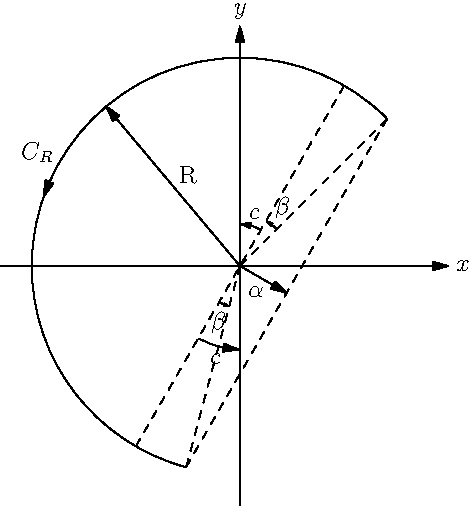
\includegraphics[width=3in]{graphics/contour_jordan.pdf}
\end{figure}
%%%%%%%%%%%%%%%%%%%%%%%%%%%%%%%%%%%%

\[
  I=\int_{C_R} e^{(be^{ic}) z} f(z) dz,
\]
then
\begin{equation} \label{E:jordan1}
  |I|\le \max_z |f(z)| \times \pi 
         \left[ \alpha e^{b\alpha}+\frac{1-e^{-bR}}{b} \right]
         \qquad \alpha\ge 0,
\end{equation}
and 
\begin{equation} \label{E:jordan2}
  |I|\le \max_z |f(z)| \times \frac{\pi}{b}
         \left[ e^{\frac{2b\alpha}{\pi}} - e^{-bR} \right]
         \qquad \alpha<0.
\end{equation}
Specifically, if $\max_z |f(z)|\to 0$ as $R\to \infty$, then
\[
  \lim_{R\to \infty} I = 0.
\]
\end{lemma}
%%%%%%%%%%%%%%%%%%%%%%%%%%%%%%%%%%
\begin{proof}
From definition we have
\[
  I=\int_{\frac{\pi}{2}-c-\beta}^{\frac{3\pi}{2}-c+\beta}
    e^{bRe^{i(\theta+c)}} f(Re^{i\theta}) iRe^{i\theta} d\theta,
\]
hence
\[
  |I| \le \max_{\theta}|f(Re^{i\theta})| \times R
          \int_{\frac{\pi}{2}-\beta}^{\frac{3\pi}{2}+\beta}
            e^{bR\cos{\theta}} d\theta
      = \max_{\theta}|f(Re^{i\theta})| \times R \times J
\]
where 
\[
  J= \int_{\frac{\pi}{2}-\beta}^{\frac{3\pi}{2}+\beta}
       e^{bR\cos{\theta}} d\theta.
\]

We first investigate the case with $\beta\ge0$ (or equivalently
$\alpha\ge 0$), note that in this case
\[
  J=\left( 
      \int_{\frac{\pi}{2}-\beta}^{\frac{\pi}{2}}
      + \int_{\frac{\pi}{2}}^{\frac{3\pi}{2}}
      + \int_{\frac{3\pi}{2}}^{\frac{3\pi}{2}+\beta}
    \right)
    e^{bR\cos{\theta}} d\theta,
\]
it is easy to see that (using variable transformation)
\[
  J= 2\int_0^{\beta} e^{bR\sin{\theta}} d\theta
      + \int_0^{\pi} e^{-bR\sin{\theta}} d\theta.
\]
Now using the fact that $\alpha=R\sin{\beta}$ and lemma \ref{L:sine} we get
\[
  \int_0^{\beta} e^{bR\sin{\theta}} d\theta
  \le \int_0^{\beta} e^{bR\sin{\beta}} d\theta
  = \beta e^{bR\sin{\beta}} \le \frac{\pi\alpha}{2R} e^{b\alpha}.
\]
And again using lemma \ref{L:sine} we get
\[
  \int_0^{\pi} e^{-bR\sin{\theta}} d\theta
  = 2\int_0^{\frac{\pi}{2}} e^{-bR\sin{\theta}} d\theta
  \le 2\int_0^{\frac{\pi}{2}} e^{-bR\frac{2\theta}{\pi}} d\theta
  = \frac{\pi}{bR} (1-e^{-bR}).
\]
Substitue these back, we get inequality \ref{E:jordan1}.

Next we look at the case with $\beta<0$ (or equivalently $\alpha<0$). We have
\[
  J= \int_{\frac{\pi}{2}-\beta}^{\frac{3\pi}{2}+\beta}
       e^{bR\cos{\theta}} d\theta
   = \int_{-\beta}^{\pi+\beta} e^{-bR\sin{\theta}} d\theta
   = 2 \int_{-\beta}^{\frac{\pi}{2}} e^{-bR\sin{\theta}} d\theta,
\]
Using Lemma \ref{L:sine}, we have
\[
  J \le 2 \int_{-\beta}^{\frac{\pi}{2}} e^{-bR\frac{2\theta}{\pi}} d\theta
    = \frac{\pi}{bR}\left( e^{\frac{2b}{\pi} R\beta} - e^{-bR} \right).
\]
Using the fact that $R|\beta|\ge R\sin{|\beta|}$ hence 
$R\beta\le R\sin{\beta}=\alpha$, we get
\[
  J \le \frac{\pi}{bR}\left( e^{\frac{2b\alpha}{\pi}} - e^{-bR} \right),
\]
and thus inequality \ref{E:jordan2}.
\end{proof}

A useful corollary for doing inverse Laplace transform is the following:
%%%%%%%%%%%%%%%%%%%%%%%%%%%
\begin{corollary} \label{C:jordan}
Let $b>0$ and let $C_R$ be a contour with radius $R$ and 
$\frac{\pi}{2}-\beta \le \theta \le \frac{3\pi}{2}+\beta$, 
if 
\[
	\lim_{R\to\infty} \max_z |f(z)| = 0,
\]
then

%%%%%%%%%%%%%%%%%%%%%%%%%%%%%%%%%%%%%%%%%
\begin{marginfigure} \label{F:cont_jordan2}
  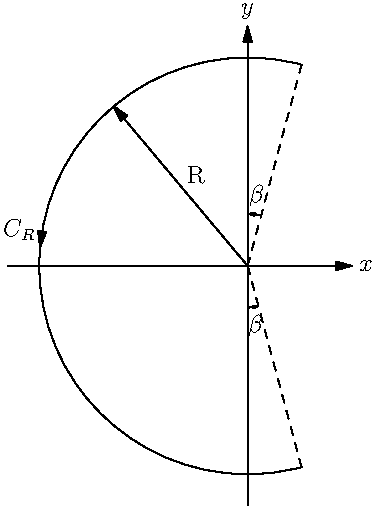
\includegraphics{graphics/contour_jordan2.pdf}
%	\caption{Contour.}
\end{marginfigure}
%%%%%%%%%%%%%%%%%%%%%%%%%%%%%%%%%%%%%%%%%

\[
  \lim_{R\to \infty} \int_{C_R} e^{b z} f(z) dz = 0.
\]
\end{corollary}
\begin{proof}
	Directly from the generalized Jordan's lemma \ref{L:jordan} with $c=0$.
\end{proof}



%%%%%%%%%%%%%%%%%%%%%%%%%%%
\begin{remark}
Here we give several special cases of the Jordan's Lemma above. Here we assume
$\max_z |f(z)|\to 0$ as $R\to \infty$, and $\beta=0$.
\begin{enumerate}
\item If $c=\pi/2$, we have
      \[
        \lim_{R\to \infty} \int_{C_R} e^{ibz} f(z) dz = 0,
      \]
      where $C_R$ is an arc in the first and/or the second quadrants.
\item If $c=-\pi/2$, we have
      \[
        \lim_{R\to \infty} \int_{C_R} e^{-ibz} f(z) dz = 0,
      \]
      where $C_R$ is an arc in the third and/or the fourth quadrants.
\item If $c=0$, we have
      \[
        \lim_{R\to \infty} \int_{C_R} e^{bz} f(z) dz = 0,
      \]
      where $C_R$ is an arc in the second and/or the third quadrants.
\item If $c=\pi$, we have
      \[
        \lim_{R\to \infty} \int_{C_R} e^{-bz} f(z) dz = 0,
      \]
      where $C_R$ is an arc in the fourth and/or the first quadrants.
\end{enumerate}
\end{remark}
           % complex variables

\chapter{Inverse Laplace Transform}

%%%%%%%%%%%%%%%%%%%%%%%%%%%%%%%%%%%%%%%%%%%%%%%%%%%%%%%
\section{Definition}
The Laplace transform $F(p)$ of a function $f(t)$ is
\begin{equation}
  F(p) = \int_0^{\infty} f(t)\, e^{-pt} dt.
\end{equation}
The inverse Laplace transform $f(t)$ of a function $F(p)$ is
\begin{equation}
	f(t) = L_p^{-1} [ F(p) ] 
       = \frac{1}{2\pi i}   
           \int_{c-i\infty}^{c+i\infty} e^{p t} F(p)\, dp
\end{equation}

It is easy to see that
\begin{align*}
	F(a p+b) 
	&= \int_0^{\infty} f(t) e^{-(a p+b)t} dt  \\
	&= \int_0^{\infty} \frac{1}{a} f\left(\tau\right) e^{-b\tau /a} 
	     e^{-p\tau} d\tau  \qquad (\tau=a t),
\end{align*}
thus
\begin{equation} \label{E:ilt_lin}
	L_p^{-1} [ F(a p + b) ] = \frac{1}{a} f(\frac{t}{a}) e^{-b t/a}.
\end{equation}

It is useful to carry out the calculation a little further for a small circle
contour such as $EFG$ in Fig. \ref{F:cont1} as it reappears frequently. Let
$C_{\rho}$ be an arc with $p=\rho e^{i\theta}$ and we have
\[
  \int_{C_{\rho}}  
    = \frac{1}{2\pi i} \lim_{\rho\to 0} 
      \int e^{\rho e^{i\theta} t} F(\rho e^{i\theta})
        \rho e^{i\theta} i d\theta
    = \frac{\rho}{2\pi} \lim_{\rho\to 0} 
      \int_{C_{\rho}} e^{\rho t (\cos\theta+i\sin\theta)} F(\rho e^{i\theta})
         e^{i\theta} d\theta,
\]
and we have the inequality
\begin{equation}
  \lim_{\rho\to 0} \left| \int_{C_{\rho}} \right| 
    \le \lim_{\rho\to 0} \frac{\rho}{2\pi} 
      \int e^{\rho t \cos\theta} \left| F(\rho e^{i\theta}) \right| d\theta
    \le \lim_{\rho\to 0} \frac{\rho}{2\pi} e^{\rho t} 
        \int \left| F(\rho e^{i\theta}) \right| d\theta.
\end{equation}
One proposition of this is that if 
$\lim_{\rho\to 0} \rho |F(\rho e^{i\theta})|=0$ then we have 
$\lim_{\rho\to 0} \int_{C_{\rho}} =0$.


%%%%%%%%%%%%%%%%%%%%%%%%%%%%%%%%%%%%%%%%%%%%%%%%%%%%%%%
\section{ $ L_p^{-1} [ e^{-a\sqrt{p}} ], a>0 $ }
From definition, 
\[
	f(t)= L_p^{-1}\left[ e^{-a\sqrt{p}} \right]
	    = \frac{1}{2\pi i} 
			  \int_{c-i\infty}^{c+\infty} 
				e^{zt} e^{-a\sqrt{z}} dz.
\]
Since $z=0$ is a branch point, we use a contour around the branch cut from
$z=-\infty$ to $z=0$ (thus remaining in the principal branch) and have

%%%%%%%%%%%%%%%%%%%%%%%%%%%%%%%%%%%%
\begin{marginfigure} 
  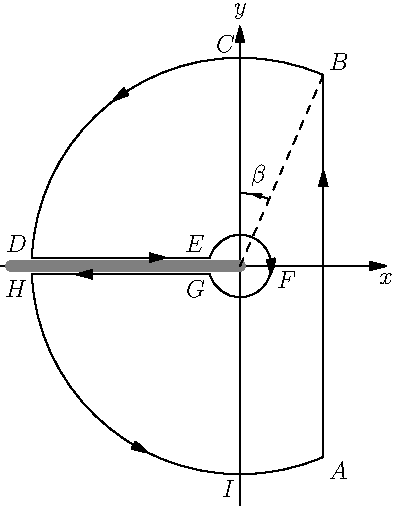
\includegraphics{graphics/contour.pdf}
\end{marginfigure}
%%%%%%%%%%%%%%%%%%%%%%%%%%%%%%%%%%%%

\[
  \oint = \int_{AB} + \int_{BCD} + \int_{DE} + \int_{EFG} + \int_{GH}
          + \int_{HIA}.
\]

Since the contour does not include any poles, using the residue theorem on the
principal branch $\sqrt{z}$ we get $\oint =0$. Now on contour $BCD$, 
$z=R e^{i\theta}$, $\frac{\pi}{2}-\beta <\theta <\pi$; while on contour $HIA$, 
$z=R e^{i\theta}$, $-\pi <\theta < -\frac{\pi}{2}+\beta$. Now on $BCD$ and
$HIA$, we have
\[
	\lim_{R\to \infty} \max_z |e^{-a\sqrt{z}}|
	= \lim_{R\to \infty} \max_{\theta} | e^{-a\sqrt{R} \cos\frac{\theta}{2}} |
	= \lim_{R\to \infty} e^{-a\sqrt{R}}
	= 0,
\]
thus by Jordan's Lemma (Corollary \ref{C:jordan}) we have
\[
  \int_{BCD} + \int_{HIA} = 0.
\]
And on the small circle contour $EFG$ we have
\[
	\int_{EFG} 
	= \frac{1}{2\pi i} 
	  \lim_{\epsilon\to 0} \int_{\pi}^{-\pi} e^{t\epsilon e^{i\theta}}
	    e^{-a\sqrt{\epsilon} e^{i\theta /2}} \epsilon e^{i\theta} i d\theta
	= 0.
\]

Along line $DE$, $z=x e^{i\pi}=-x$, where $x$ ranges from $\infty$ to $0$, and 
$\sqrt{z}=\sqrt{x} e^{i\pi /2}= i\sqrt{x}$, thus
\[
	\int_{DE} = \frac{1}{2\pi i} \int_{\infty}^0 e^{-tx} e^{-i a \sqrt{x}} (-dx).
\]
Similarly, along line $GH$, $z=x e^{-i\pi}=-x$, where $x$ ranges from $0$ to
$\infty$, and $\sqrt{z}=\sqrt{x} e^{-i\pi/2} = -i\sqrt{x}$, thus 
\[
	\int_{GH} = \frac{1}{2\pi i} \int^{\infty}_0 e^{-tx} e^{i a \sqrt{x}} (-dx).
\]
Hence
\[
	\int_{DE} + \int_{GH}
	= -\frac{1}{\pi} \int_0^{\infty} e^{-tx} \sin a\sqrt{x} dx
	= -\frac{2}{\pi t} 
	  \int_0^{\infty} e^{-u^2} \sin \left( \frac{a}{\sqrt{t}} u \right) u du,
\]
using Eq. \ref{E:int2_2}, we have
\[
	\int_{DE} + \int_{GH}
	= - \frac{a}{2\sqrt{\pi} t^{3/2}} e^{-a^2/4t}.
\]

Hence 
\begin{align*}
  \int_{AB} 
	&= \oint - \left( \int_{BCD} + \int_{HIA} \right)
     - \left( \int_{DE} + \int_{GH} \right) - \int_{EFG}  \\
  &= \frac{a}{2\sqrt{\pi} t^{3/2}} e^{-a^2/4t}, 
\end{align*}
i.e.
\footnote{cf. Borodin and Salemin, Handbook of Brownian Motions, 2ed, Appendix
3.2, Equation 2, p. 650}
\begin{equation} \label{E:ilt_1a}
	f(t)= L_p^{-1}\left[ e^{-a\sqrt{p}} \right]
      = \frac{a}{2\sqrt{\pi} t^{3/2}} e^{-a^2/4t}, \qquad a>0.
\end{equation}

%%%%%%%%%%%%%%%%%%%%%%%%%%%%%%%%%%%%%%%%%%%%%%%%%%%%%%%
\section{$ L_{\lambda}^{-1} 
\left( \frac{e^{-\alpha \sqrt{2\lambda}}}{\lambda(\sqrt{2\lambda}+\gamma)}
\right), \alpha > 0 $}
Let
\begin{align*}
  f(y) &= L_{\lambda}^{-1} 
          \left( 
            \frac{e^{-\alpha \sqrt{2\lambda}}}{\lambda(\sqrt{2\lambda}+\gamma)} 
          \right)    \\
       &= \frac{1}{2\pi i}   
           \int_{c-i\infty}^{c+i\infty} e^{\lambda y} 
           \frac{e^{-\alpha \sqrt{2\lambda}}}{\lambda(\sqrt{2\lambda}+\gamma)} 
           \, d\lambda.
\end{align*}
Since $\lambda=0$ is a branch point, we use the contour shown in Figure
\ref{F:cont1} and have
\[
  \oint = \int_{AB} + \int_{BCD} + \int_{DE} + \int_{EFG} + \int_{GH}
          + \int_{HIA}.
\]
Using the residue theorem (on the principal branch $\sqrt{\lambda}$) we get 
$\oint=0$. Using Jordan's Lemma we see
\[
  \int_{BCD} + \int_{HIA} = 0.
\]
%(remark that for contour HIA $F(\lambda)=
%\frac{e^{\alpha \sqrt{2\lambda}}}{\lambda(-\sqrt{2\lambda}+\gamma)}$).


%%%%%%%%%%%%%%%%%%%%%%%%%%%%%%%%%%%%
% \begin{figure} \label{F:cont1}
%   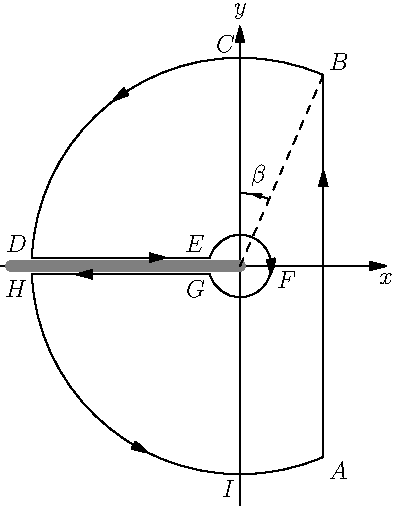
\includegraphics[width=3in]{graphics/contour.pdf}
% \end{figure}
\begin{marginfigure} \label{F:cont1}
  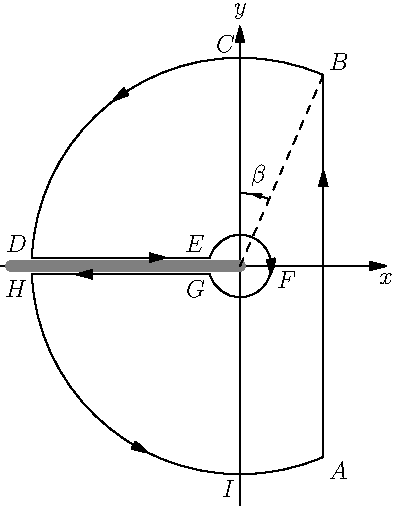
\includegraphics{graphics/contour.pdf}
	\caption{Contour.}
\end{marginfigure}
%%%%%%%%%%%%%%%%%%%%%%%%%%%%%%%%%%%%


It is easy to see that
\[
  \int_{EFG} = \frac{1}{2\pi i} \lim_{\epsilon \to 0} 
    \int_{\pi}^{-\pi} 
    \frac{ e^{ y \epsilon e^{i\theta} - \sqrt{2\epsilon} e^{i\theta/2} \alpha } }
         { \epsilon e^{i\theta} (\sqrt{2\epsilon} e^{i\theta/2} + \gamma) }
    \epsilon e^{i\theta} i d\theta
   = - \frac{1}{\gamma}.
\]
Along line $DE$, let $\lambda=x e^{i\pi}=-x$, 
and $\sqrt{2\lambda}=\sqrt{2x} e^{i\pi /2}=i \sqrt{2x}$, we get
\[
  \int_{DE} = \frac{1}{2\pi i} 
    \int_{\infty}^0 \frac{e^{-xy}}{x}\, 
      \frac{e^{-i\alpha\sqrt{2x}}}{\gamma+i\sqrt{2x}}\, dx.
\]
Similarly, along line $GH$, let $\lambda=x e^{-i\pi}=-x$, 
and $\sqrt{2\lambda}=\sqrt{2x} e^{-i\pi /2}=-i \sqrt{2x}$, we get
\[
  \int_{GH} = \frac{1}{2\pi i} 
    \int^{\infty}_0 \frac{e^{-xy}}{x}\, 
      \frac{e^{i\alpha\sqrt{2x}}}{\gamma-i\sqrt{2x}}\, dx.
\]
Hence
\begin{align*}
  \int_{DE} + \int_{GH} 
  &= \frac{1}{\pi} \int_0^{\infty} \frac{e^{-yx}}{x(\gamma^2+2x)}
       \left[
         \gamma \sin(\alpha \sqrt{2x}) + \sqrt{2x} \cos(\alpha \sqrt{2x})
       \right] \, dx  \\
  &= \frac{2\gamma}{\pi} \int_0^{\infty} 
       \frac{e^{-yu^2/2} \sin(\alpha u)}{u(u^2+\gamma^2)} \, du
     + \frac{2}{\pi} \int_0^{\infty} 
       \frac{e^{-yu^2/2} \cos(\alpha u)}{u^2+\gamma^2} \, du
\end{align*}
Using Equations \ref{E:int3} and \ref{E:int5}, we get
\[
  \int_{DE} + \int_{GH} 
  = \frac{1}{\gamma} e^{\alpha \gamma+\frac{1}{2}\gamma^2 y} 
      \erfc \left( \frac{\gamma \sqrt{y}}{\sqrt{2}}+ \frac{\alpha}{\sqrt{2y}} \right)
    + \frac{1}{\gamma} - \frac{1}{\gamma} \erfc \left( \frac{\alpha}{\sqrt{2y}}
\right).
\]
Hence 
\begin{align*}
  \int_{AB} &= \oint - \left( \int_{BCD} + \int_{HIA} \right)
               - \left( \int_{DE} + \int_{GH} \right) - \int_{EFG}  \\
            &= \frac{1}{\gamma} \erfc \left( \frac{\alpha}{\sqrt{2y}} \right)
               - \frac{1}{\gamma} e^{\alpha \gamma+\frac{1}{2}\gamma^2 y} 
                 \erfc 
                   \left( 
                     \frac{\gamma \sqrt{y}}{\sqrt{2}} + \frac{\alpha}{\sqrt{2y}} 
                   \right)
\end{align*}
This is exactly the inverse Laplace transform we are looking for
\begin{align} \label{E:ilt1}
  f(y) &= L_{\lambda}^{-1} 
          \left( 
            \frac{e^{-\alpha \sqrt{2\lambda}}}{\lambda(\sqrt{2\lambda}+\gamma)} 
          \right)   \notag \\  
       &= \frac{1}{\gamma} \erfc \left( \frac{\alpha}{\sqrt{2y}} \right)
          - \frac{1}{\gamma} e^{\alpha \gamma+\frac{1}{2}\gamma^2 y} 
            \erfc 
              \left( 
                \frac{\gamma \sqrt{y}}{\sqrt{2}}+ \frac{\alpha}{\sqrt{2y}} 
              \right)
\end{align}


%%%%%%%%%%%%%%%%%%%%%%%%%%%%%%%%%%%%%%%%%%%%%%%%%%%%%%%%%%%%%%%%%%%%%%%%%%%%%%%%
\section{$ L_{\lambda}^{-1}[ 
  \frac{1}{\sqrt{\lambda}} e^{-\alpha \sqrt{\lambda}} ] $ }
Use the same contour as in Figure \ref{F:cont1}, we get
\[
  \oint = \int_{AB} + \int_{BCD} + \int_{DE} + \int_{EFG} + \int_{GH}
          + \int_{HIA}.
\]
It is easy to see that $\oint=0$. Using Jordan's lemma, we have
\[
  \int_{BCD} + \int_{HIA} = 0.
\]
And
\[
  \int_{EFG} = \frac{1}{2\pi i} \lim_{\epsilon \to 0} 
    \int_{\pi}^{-\pi} e^{\epsilon e^{i\theta} y}
    \frac{1}{\sqrt{\epsilon} e^{i\theta/2}}
    e^{-\alpha \sqrt{\epsilon} e^{i\theta/2}}
    \epsilon e^{i\theta} \, i d\theta
  = 0. 
\]
Along line $DE$, let $\lambda=x e^{i\pi}=-x$, and 
$\sqrt{\lambda}=\sqrt{x} e^{i\pi/2}=i\sqrt{x}$, we get
\[
  \int_{DE} = -\frac{1}{2\pi} \int_0^{\infty} \frac{e^{-xy}}{\sqrt{x}}
              e^{-i\alpha x} \, dx.
\]
Similarly, along line $GH$, let $\lambda=x e^{-i\pi}=-x$, and 
$\sqrt{\lambda}=\sqrt{x} e^{-i\pi/2}=-i\sqrt{x}$, we get
\[
  \int_{GH} = -\frac{1}{2\pi} \int_0^{\infty} \frac{e^{-xy}}{\sqrt{x}}
              e^{i\alpha x} \, dx.
\]
Hence (using Equation \ref{E:int2} for the last step)
\begin{align*}
  \int_{DE} + \int_{GH} 
    &= -\frac{1}{2\pi} \int_0^{\infty} \frac{e^{-xy}}{\sqrt{x}}
       \left( e^{i\alpha x} + e^{-i\alpha x} \right) \, dx \\
    &= -\frac{1}{\pi} \int_0^{\infty} \frac{e^{-xy}}{\sqrt{x}}
         cos(\alpha \sqrt{x}) \, dx   \\
    &= - \frac{2}{\pi} \int_0^{\infty} e^{-yu^2} cos(\alpha u) \, du  \\
    &= - \frac{1}{\sqrt{\pi y}} e^{-\frac{\alpha^2}{4y}}
\end{align*}
Take all together and note that $f(y)=\int_{AB}$, we get
\begin{equation} \label{E:ilt2}
  f(y) = L_{\lambda}^{-1} 
         \left[ 
           \frac{1}{\sqrt{\lambda}} e^{-\alpha \sqrt{\lambda}}
         \right]
    = \frac{1}{\sqrt{\pi y}} e^{ -\frac{\alpha^2}{4y} } 
\end{equation}


%%%%%%%%%%%%%%%%%%%%%%%%%%%%%%%%%%%%%%%%%%%%%%%%%%%%%%
\section{ $ L_p^{-1} [ \frac{1}{\sqrt{p}(\sqrt{p}+b)} e^{-a\sqrt{p}} ], a\ge 0 $ }
From definition, 
\[
	f(t)= L_p^{-1}\left[ \frac{e^{-a\sqrt{p}}}{\sqrt{p}(\sqrt{p}+b)} \right]
	    = \frac{1}{2\pi i} 
			  \int_{c-i\infty}^{c+\infty} 
				e^{zt} \frac{e^{-a\sqrt{z}}}{\sqrt{z}(\sqrt{z}+b)} dz.
\]
Since $z=0$ is a branch point, we use a contour around the branch cut from
$z=-\infty$ to $z=0$ (thus remaining in the principal branch) and have

%%%%%%%%%%%%%%%%%%%%%%%%%%%%%%%%%%%%
\begin{marginfigure} 
  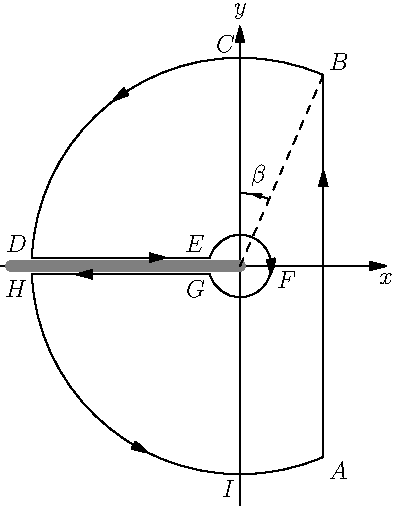
\includegraphics{graphics/contour.pdf}
\end{marginfigure}
%%%%%%%%%%%%%%%%%%%%%%%%%%%%%%%%%%%%

\[
  \oint = \int_{AB} + \int_{BCD} + \int_{DE} + \int_{EFG} + \int_{GH}
          + \int_{HIA}
\]

Since the contour does not include any poles, using the residue theorem on the
principal branch $\sqrt{z}$ we get $\oint =0$. 

Now on contour $BCD$, 
$z=R e^{i\theta}$, $\frac{\pi}{2}-\beta <\theta <\pi$; while on contour $HIA$, 
$z=R e^{i\theta}$, $-\pi <\theta < -\frac{\pi}{2}+\beta$. On $BCD$ and
$HIA$, we have
\[
  \lim_{R\to \infty} 
    \max_z \left| \frac{e^{-a\sqrt{z}}}{\sqrt{z}(\sqrt{z}+b)} \right|
  = \lim_{R\to \infty} \max_{\theta} 
      \left| 
        \frac{e^{-a\sqrt{R} e^{i\theta/2}}}
             { \sqrt{R} e^{i\theta/2} (\sqrt{R} e^{i\theta/2} + b) }
      \right|
  = 0,
\]
thus by Jordan's Lemma (Corollary \ref{C:jordan}) we have
\[
  \int_{BCD} + \int_{HIA} = 0.
\]
And on the small circle contour $EFG$ we have
\[
	\int_{EFG} 
	= \frac{1}{2\pi i} 
	  \lim_{\epsilon\to 0} \int_{\pi}^{-\pi} e^{t\epsilon e^{i\theta}}
	    \frac{e^{-a\sqrt{\epsilon} e^{i\theta/2}}}
             { \sqrt{\epsilon} e^{i\theta/2} (\sqrt{\epsilon} e^{i\theta/2} + b)}
        \epsilon e^{i\theta} i d\theta
	= 0.
\]

Along line $DE$, $z=x e^{i\pi}=-x$, where $x$ ranges from $\infty$ to $0$, and 
$\sqrt{z}=\sqrt{x} e^{i\pi /2}= i\sqrt{x}$, thus
\[
	\int_{DE} = \frac{1}{2\pi i} 
      \int_{\infty}^0 e^{-tx} 
        \frac{e^{-i a \sqrt{x}}}{i\sqrt{x}(i\sqrt{x}+b)} (-dx).
\]
Similarly, along line $GH$, $z=x e^{-i\pi}=-x$, where $x$ ranges from $0$ to
$\infty$, and $\sqrt{z}=\sqrt{x} e^{-i\pi/2} = -i\sqrt{x}$, thus 
\[
	\int_{GH} = \frac{1}{2\pi i}  
      \int^{\infty}_0 e^{-tx} 
        \frac{e^{i a \sqrt{x}}}{-i\sqrt{x}(-i\sqrt{x}+b)} (-dx).
\]
Hence
\begin{align*}
  \int_{DE} + \int_{GH}
	&= \frac{1}{\pi} 
      \int_0^{\infty} \frac{e^{-tx}}{\sqrt{x}(x+b^2)} 
        \left[ \sqrt{x}\sin(a\sqrt{x}) - b\cos(a\sqrt{x}) \right] dx \\
  &= \frac{2}{\pi} 
       \int_0^{\infty} \frac{e^{-t u^2} \sin(a u)}{u^2+b^2} \, u du
     -\frac{2b}{\pi} 
       \int_0^{\infty} \frac{e^{-t u^2} \cos(a u)}{u^2+b^2} \, du
\end{align*}
Using Equations \ref{E:int3} and \ref{E:int4}, we get
\[
  \int_{DE} + \int_{GH}
    = -e^{a b + b^2 t} \erfc\left( \frac{a}{2\sqrt{t}} + b \sqrt{t} \right)
\]

Hence 
\begin{align*}
  \int_{AB} 
	&= \oint - \left( \int_{BCD} + \int_{HIA} \right)
     - \left( \int_{DE} + \int_{GH} \right) - \int_{EFG}  \\
  &= e^{a b + b^2 t} \erfc\left( \frac{a}{2\sqrt{t}} + b \sqrt{t} \right)
\end{align*}
i.e.
\footnote{cf. Borodin and Salemin, Handbook of Brownian Motions, 2ed, Appendix
3.2, Equation 11, p. 650}
\begin{equation} \label{E:ilt_1a}
  f(t) = L_p^{-1} \left[ \frac{1}{\sqrt{p}(\sqrt{p}+b)} e^{-a\sqrt{p}} \right]
       = e^{a b + b^2 t} \erfc\left( \frac{a}{2\sqrt{t}} + b \sqrt{t} \right),
         \qquad a\ge 0 
\end{equation}



%%%%%%%%%%%%%%%%%%%%%%%%%%%%%%%%%%%%%%%%%%%%%%%%%%%%%%%%%%%%%%%%%%%%%%%%%%%%%%%%
\section{$ L_{\lambda}^{-1}[ 
  \frac{1}{\lambda} e^{-\alpha \sqrt{\lambda}} ] $ }
Let
\begin{align*}
  f(y) &= L_{\lambda}^{-1} 
          \left( 
            \frac{1}{\lambda} e^{-\alpha \sqrt{\lambda}} 
          \right)    \\
       &= \frac{1}{2\pi i}   
          \int_{c-i\infty}^{c+i\infty} e^{\lambda y} 
            \frac{1}{\lambda} e^{-\alpha \sqrt{\lambda}}  
            \, d\lambda.
\end{align*}
Since $\lambda=0$ is a branch point, we use the contour shown in Figure
\ref{F:cont1} and have
\[
  \oint = \int_{AB} + \int_{BCD} + \int_{DE} + \int_{EFG} + \int_{GH}
          + \int_{HIA}.
\]
Using the residue theorem (on the principal branch $\sqrt{\lambda}$) we get 
$\oint=0$. Using Jordan's Lemma we get
\[
  \int_{BCD} + \int_{HIA} = 0.
\]
It is easy to see that 
\[
  \int_{EFG} = \lim_{\epsilon \to 0} \frac{1}{2\pi i}
               \int_{\pi}^{-\pi} e^{y \epsilon e^{i\theta}}
               \frac{1}{\epsilon e^{i\theta}}
               e^{-\alpha \sqrt{\epsilon} e^{i\theta/2}}
               \epsilon e^{i\theta} i \, d\theta
             = -1.
\]
Along line $DE$, let $\lambda=x e^{i\pi}=-x$, and 
$\sqrt{\lambda}=\sqrt{x} e^{i\pi/2}=i\sqrt{x}$, we get
\[
  \int_{DE} = -\frac{1}{2\pi i} \int_0^{\infty} \frac{e^{-xy}}{x}
              e^{-i\alpha x} \, dx.
\]
Similarly, along line $GH$, let $\lambda=x e^{-i\pi}=-x$, and 
$\sqrt{\lambda}=\sqrt{x} e^{-i\pi/2}=-i\sqrt{x}$, we get
\[
  \int_{GH} = \frac{1}{2\pi i} \int_0^{\infty} \frac{e^{-xy}}{x}
              e^{i\alpha x} \, dx.
\]
Hence
\begin{align*}
  \int_{DE} + \int_{GH} 
    &= \frac{1}{\pi} 
      \int_0^{\infty} \frac{ e^{-xy} }{ x } \sin( \alpha \sqrt{x} ) \, dx \\
    &= \frac{2}{\pi} \int_0^{\infty} \frac{e^{-yu^2}}{u} \sin(\alpha u) \, du
\end{align*}
Using Equation \ref{E:int3} with $\gamma=0$, we get
\[
  \int_{DE} + \int_{GH} 
    =   \frac{1}{2} \erfc \left( -\frac{\alpha}{2\sqrt{y}} \right)
      - \frac{1}{2} \erfc \left( \frac{\alpha}{2\sqrt{y}}  \right).
\]

Hence 
\begin{align*}
  \int_{AB} 
	&= \oint - \left( \int_{BCD} + \int_{HIA} \right)
     - \left( \int_{DE} + \int_{GH} \right) - \int_{EFG}  \\
    & = 1 - \frac{1}{2} \erfc \left( -\frac{\alpha}{2\sqrt{y}} \right)
          + \frac{1}{2} \erfc \left( \frac{\alpha}{2\sqrt{y}}  \right) \\
    &= \erfc \left( \frac{\alpha}{2\sqrt{y}} \right) 
\end{align*}
i.e.
\footnote{cf. Borodin and Salemin, Handbook of Brownian Motions, 2ed, Appendix
3.2, Equation 6, p. 650}
\begin{equation}  \label{E:ilt3}
  f(y) = L_{\lambda}^{-1} 
         \left[ 
           \frac{1}{\lambda} e^{-\alpha \sqrt{\lambda}}
         \right]
       = \erfc \left( \frac{\alpha}{2\sqrt{y}} \right).
\end{equation}


%%%%%%%%%%%%%%%%%%%%%%%%%%%%%%%%%%%%%%%%%%%%%%%%%%%%%%%%%%%%%%%%%%%%%%%%
\section{$L_p^{-1}[ \erfc(\sqrt{ap}) ] $ }
Let 
\[
  F(p) = \erfc(\sqrt{ap}) 
       = \frac{2}{\sqrt{\pi}} \int_{\sqrt{ap}}^{\infty} e^{-x^2} dx,
\]
and we have
\[
  \frac{dF}{dp} = - \sqrt{\frac{a}{\pi}} \frac{e^{-ap}}{\sqrt{p}},
\]
and
\[
  \frac{d^2F}{dp^2} = \sqrt{\frac{a}{\pi}} \frac{e^{-ap}}{\sqrt{p}} 
                      \left( a + \frac{1}{2p} \right).
\]
Hence
\[
  p F"(p) + 2 F'(p) = a (-p F'(p) - F(p) ) + \frac{3}{2} F'(p) + a F(p),
\]
and the inverse Laplace transform of this equation is
\[
  (t^2-a t) f'(t) = (a-\frac{3}{2} t) f(t),
\]
where $f(t)$ is the inverse Laplace transform of function $F(p)$.
Solve this differential equation, we get
\[
  f(t) = \frac{A}{t \sqrt{t-a}} 1_{(a,\infty)}(t),
\]
here $A$ is the constant to be determined and we have used the fact that
$f(0)=\lim_{p \to \infty} p F(p) = 0$.

To determine the constant $A$, we take the Laplace transform of function
$\frac{A}{t \sqrt{t-a}} 1_{(a,\infty)}(t)$, this yields (using Equation
\ref{E:int6})
\[
  L\left[ f(t) = \frac{A}{t \sqrt{t-a}} 1_(a,\infty)(t) \right]
    = \frac{A}{\sqrt{a}} \int_1^{\infty} \frac{e^{-(ap)x}}{x \sqrt{x-1}} dx
    = \frac{A}{\sqrt{a}} \pi \erfc(\sqrt{ap}).
\]
Since this should be $\erfc(\sqrt{ap})$, we must have
$A=\sqrt{a}/\pi$, and 
\begin{equation}
  L_p^{-1}[ \erfc(\sqrt{ap}) ] = \frac{\sqrt{a}}{\pi t \sqrt{t-a}}
                                 1_{(a,\infty)}(t).
\end{equation}


%%%%%%%%%%%%%%%%%%%%%%%%%%%%%%%%%%%%%%%%%%%%%%%%%%%%%%%%%%%%%%%%%%%%%%%%
\section{$L_p^{-1}[ p^{-\nu} ], \nu>0 $ }
To invert function $p^{-\nu}$ for any $\nu>0$, first note that
for all positive integer $n$ we have
\[
  L_p^{-1} \left[ \frac{d^n}{dp^n} F(p) \right] = (-t)^n f(t).
\]
Thus for any $\nu>0$ let $n$ be the integral part of $\nu$ we have
\begin{align*} 
  L_p^{-1}[p^{-\nu}] 
    &= \left( \frac{-}{\nu-1} \right) 
        L_p^{-1} \left[\frac{d}{dp} p^{-(\nu-1)} \right] \notag \\
    &= \left( \frac{-}{\nu-1} \right) \left( \frac{-}{\nu-2} \right) 
        L_p^{-1} \left[\frac{d^2}{dp^2} p^{-(\nu-2)} \right] \notag \\
    &= \cdots  \notag \\
    &= \left( \frac{-}{\nu-1} \right) \left( \frac{-}{\nu-2} \right) 
       \cdots \left( \frac{-}{\nu-n} \right) 
        L_p^{-1} \left[\frac{d^n}{dp^n} p^{-(\nu-n)} \right], \notag \\
    &= \left( \frac{1}{\nu-1} \right) \left( \frac{1}{\nu-2} \right) 
       \cdots \left( \frac{1}{\nu-n} \right) 
       t^n L_p^{-1} \left[ p^{-(\nu-n)} \right], \notag \\
\end{align*}
that is
\begin{equation} \label{E:ilt_pow}
  L_p^{-1}[p^{-\nu}] 
    = \left( \frac{1}{\nu-1} \right) \left( \frac{1}{\nu-2} \right) 
      \cdots \left( \frac{1}{\nu-n} \right) 
      t^n L_p^{-1} \left[ p^{-(\nu-n)} \right].
\end{equation}
Hence we only need to invert the function with $0<\nu<1$.

To invert function $F(p)=p^{-\nu}$ with $0<\nu<1$ by contour integration we have
\[
  f(t) = L_p^{-1} \left[ p^{-\nu} \right]
       = \frac{1}{2\pi i}   
           \int_{c-i\infty}^{c+i\infty} e^{p t} p^{-\nu}\, dp
       = t^{\nu-1} 
           \frac{1}{2\pi i} \int_{c-i\infty}^{c+i\infty} e^{z} z^{-\nu}\, dz,
\]
For simplicity we use the notation
\[
   \int_{AB} = \frac{1}{2\pi i} \int_{AB} e^{z} z^{-\nu}\, dz,
\]
and similarly for integration over other contours.
Since $z=0$ is a branch point (in general) we use the following contour and 
from the residue theorem we have

%%%%%%%%%%%%%%%%%%%%%%%%%%%%%%%%%%%%
\begin{marginfigure} \label{F:cont2}
  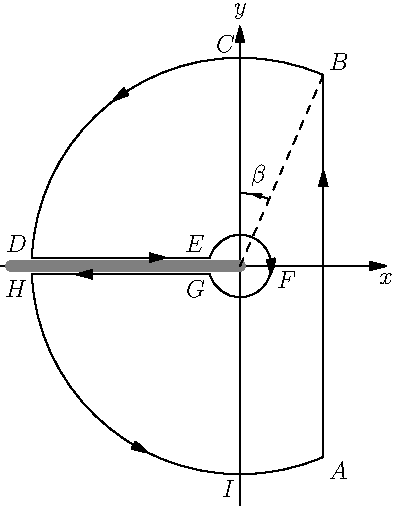
\includegraphics{graphics/contour.pdf}
\end{marginfigure}
%%%%%%%%%%%%%%%%%%%%%%%%%%%%%%%%%%%%

\[
  \oint = \int_{AB} + \int_{BCD} + \int_{DE} + \int_{EFG} + \int_{GH}
          + \int_{HIA} = 0.
\]

Note that from Jordan's lemma \ref{L:jordan} we have 
\[
  \int_{BCD}  + \int_{HIA} = 0.
\]
We also have $\int_{EFG}=0$ because
\[
  \lim_{\epsilon\to 0} |\int_{EFG} z^{-\nu} e^{z t} dz|
    \le \lim_{\epsilon\to 0} \int_{\pi}^{-\pi} \epsilon^{1-\nu} e^{\epsilon
        t\cos \theta} d\theta 
    = 0
\]
Along $DE$, $z=x e^{i\pi}$, thus
\[
  \frac{1}{2\pi i} \int_{DE} z^{-\nu} e^z dz
    = \frac{e^{-i\pi\nu}}{2\pi i} \int_0^{\infty} x^{-\nu} e^x dx,
\]
while along $GH$, $z=x e^{-i\pi}$, thus
\[
  \frac{1}{2\pi i} \int_{GH} z^{-\nu} e^z dz
    = - \frac{e^{i\pi\nu}}{2\pi i} \int_0^{\infty} x^{-\nu} e^x dx.
\]
Hence
\[
  \int_{DE} + \int_{GH}
    = - \frac{\sin(\nu\pi)}{\pi} \int_0^{\infty} x^{-\nu} e^x dx
    = - \frac{\sin(\nu\pi)}{\pi} \Gamma(1-\nu).
\]
and 
\[
  L_p^{-1} \left[ p^{-\nu} \right] = t^{\nu-1} \int_{AB}
    = \frac{\sin(\nu\pi)}{\pi} \Gamma(1-\nu).
\]
Using the Euler's reflection formula for gamma function (Proposition
\ref{P:gamma_pp}) we have
\begin{equation}
  L_p^{-1} \left[ p^{-\nu} \right] 
    = \frac{t^{\nu-1}}{\Gamma(\nu)}, \qquad 0<\nu<1.
\end{equation}

Using Eq. \ref{E:ilt_pow} and the simple property of gamma function
$\Gamma(z)=z\Gamma(z-1)$ we get
\begin{equation} \label{E:ilt4}
  L_p^{-1} \left[ p^{-\nu} \right] 
    = \frac{t^{\nu-1}}{\Gamma(\nu)}, \qquad \nu>0.
\end{equation}

%%%%%%%%%%%%%%%%%%%%%%%%%%%%%%%%%%%%%%%%%%%%%%%%%%%%%%%%%%%%%%%%%%%%%%%%
\section{$L_p^{-1}[ p^{-\mu} e^{a/p} ], \mu>0 $ }
Using Eq. \ref{E:ilt4} we get 
\begin{align*}
  L_p^{-1} \left[ p^{-\mu} e^{a/p} \right]
    &= L_p^{-1} 
       \left[ p^{-\mu} 
         \sum_{m=0}^{\infty} \left( \frac{a}{p} \right)^m \frac{1}{m!}
       \right]  \notag \\
    &= \sum_{m=0}^{\infty} \frac{a^m}{m!}
       L_p^{-1} \left[ \frac{1}{p^{m+\mu}} \right]  \notag \\
    &= \sum_{m=0}^{\infty} \frac{a^m}{m!}
       \frac{t^{\mu+m-1}}{\Gamma(\mu+m)}      \notag \\
    &= t^{\mu-1} \sum_{m=0}^{\infty} \frac{a^m t^m}{m!\Gamma(\mu+m)}. \notag\\
\end{align*}

From the definition of the modified Bessel function $I_{\nu}(z)$
\ref{D:bessel_mod}
we get
\begin{equation} \label{E:ilt5}
  L_p^{-1} \left[ p^{-\mu} e^{a/p} \right]
    = \left( \frac{t}{a} \right)^{\frac{\mu-1}{2}} I_{\mu-1}(2\sqrt{at})
      \qquad \mu>0.   
\end{equation}

An alternative method is to use differential equations.


%%%%%%%%%%%%%%%%%%%%%%%%%%%%%%%%%%%%%%%%%%%%%%%%%%%%%%%%%%%%%%%%%%%%%%%%
\section{$L_p^{-1}[ I_{\nu}(a\sqrt{2p}) K_{\nu}(b\sqrt{2p}) ]$ }
From the defintion we have
\[
  f(t)=L_p^{-1} \left[ I_{\nu}(a\sqrt{2p}) K_{\nu}(b\sqrt{2p}) \right]
   = \frac{1}{2\pi i}  \int_{c-i\infty}^{c+i\infty}
     e^{zt} I_{\nu}(a\sqrt{2z}) K_{\nu}(b\sqrt{2z})\, dz,
\]
Since $z=0$ is a branch point (in general) we use the following contour and 
from the residue theorem we have

\[
  \oint = \int_{AB} + \int_{BCD} + \int_{DE} + \int_{EFG} + \int_{GH}
          + \int_{HIA} = 0,
\]

%%%%%%%%%%%%%%%%%%%%%%%%%%%%%%%%%%%%
\begin{marginfigure} \label{F:cont3}
  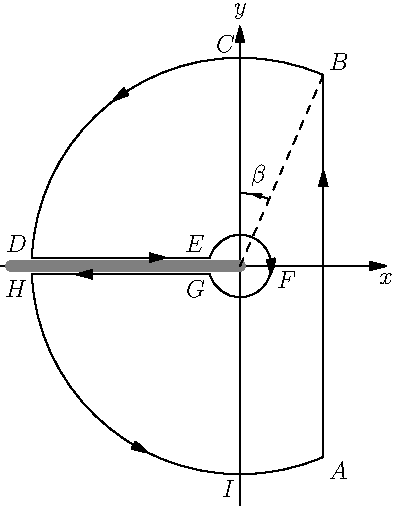
\includegraphics{graphics/contour.pdf}
\end{marginfigure}
%%%%%%%%%%%%%%%%%%%%%%%%%%%%%%%%%%%%

where for simplicity we use the notation
\[
   \int_{AB} = \frac{1}{2\pi i} 
      \int_{AB} e^{zt} I_{\nu}(a\sqrt{2z}) K_{\nu}(b\sqrt{2z})\, dz,
\]
and similarly for integration over other contours. 

First note that when $z\to\infty$ we have
\footnote{NIST Handbook of Mathematical Functions, 10.40.6 }
\[
  I_{\nu}(z) K_{\nu}(z) \sim \frac{1}{2z},
\]
thus from Jordan's lemma \ref{L:jordan} we have 
\[
  \int_{BCD}  + \int_{HIA} = 0,
\]

And note that when $z\to 0$ we have 
\[
  I_{\nu}(z) \sim \frac{1}{\Gamma(\nu+1)} \left( \frac{z}{2} \right)^{\nu},
\]
and
\[
  K_{\nu}(z) \sim \frac{\Gamma(|\nu|)}{2} \left( \frac{z}{2} \right)^{-|\nu|},
\]
hence when $\nu>-1$ we also have
\[
  \int_{EFG} = 0.
\]

Along $DE$, $z=x e^{i\pi}$, thus
\[
  \int_{DE} = \frac{1}{2\pi i} \int_0^{\infty} e^{-xt} 
    I_{\nu}(e^{i\pi/2} a\sqrt{2x}) K_{\nu}(e^{i\pi/2} b\sqrt{2x}) dx,
\]
while along $GH$, $z=x e^{-i\pi}$, thus
\[
  \int_{GH} = - \frac{1}{2\pi i} \int_0^{\infty} e^{-xt} 
    I_{\nu}(e^{-i\pi/2} a\sqrt{2x}) K_{\nu}(e^{-i\pi/2} b\sqrt{2x}) dx,
\]
Hence
\[
  \int_{DE} + \int_{GH} = - \frac{1}{2\pi i} 
    \int_0^{\infty} e^{-xt} 
    [ I_{\nu}(e^{-i\pi/2} a\sqrt{2x}) K_{\nu}(e^{-i\pi/2} b\sqrt{2x}) 
     - I_{\nu}(e^{i\pi/2} a\sqrt{2x}) K_{\nu}(e^{i\pi/2} b\sqrt{2x}) ] dx,
\]

From the definition of Bessel functions $J_{\nu}(z)$ and modified Bessel
functions $I_{\nu}(z)$ we get
\[
  I_{\nu}(e^{i\pi n/2} z) = e^{i\pi n\nu/2} J_{\nu}(z),
    \qquad n=\pm 1,\pm 3, \pm 5,\cdots
\]
Using this and the definition
$K_{\nu}(z)=\frac{\pi}{2\sin\pi\nu}(I_{-\nu}(z)-I_{\nu}(z))$ we thus get
\[
  I_{\nu}(e^{-i\pi/2} a\sqrt{2x}) K_{\nu}(e^{-i\pi/2} b\sqrt{2x}) 
    - I_{\nu}(e^{i\pi/2} a\sqrt{2x}) K_{\nu}(e^{i\pi/2} b\sqrt{2x}) 
  = i \pi \, J_{\nu}(a\sqrt{2x}) J_{\nu}(b\sqrt{2x}),
\]
and thus
\[
  f(t)= \int_{AB} = - \int_{DE} - \int_{GH} = \frac{1}{2} 
    \int_0^{\infty} e^{-xt} J_{\nu}(a\sqrt{2x}) J_{\nu}(b\sqrt{2x}) dx.
\]
Using Weber's second exponential integral
\footnote{Watson, A Treatise on the Theory of Bessel Functions, 13.31(1), p395}
\[
  \int_0^{\infty} e^{-p^2 t^2} J_{\nu}(at) J_{\nu}(bt)tdt
    = \frac{1}{2p^2} \exp\left( -\frac{a^2+b^2}{4p^2} \right)
      I_{\nu}\left( \frac{ab}{2p^2} \right)
      \qquad Re(\nu)>-1, |\arg p|<\pi/4
\]
we thus get
\begin{equation} \label{E:ilt6}
  L_p^{-1} \left[ I_{\nu}(a\sqrt{2p}) K_{\nu}(b\sqrt{2p}) \right]
    = \frac{1}{2t} \exp\left( -\frac{a^2+b^2}{2t} \right)
      I_{\nu} \left( \frac{ab}{t} \right) \qquad \nu>-1.
\end{equation}

%%%%%%%%%%%%%%%%%%%%%%%%%%%%%%%%%%%%%%%%%%%%%%%%%%%%%%%%%%%%%%%%%%%%%%%%%%
\section{$L_p^{-1}[ \frac{\sinh (\sqrt{p} a)}{\sinh (\sqrt{p} b)} ], |a|<b$ }
From definition we have
\[
  f(t)= L_p^{-1}\left[ \frac{\sinh (\sqrt{p} a)}{\sinh (\sqrt{p} b)} \right]
	    = \frac{1}{2\pi i} 
			  \int_{c-i\infty}^{c+\infty} 
		      e^{zt} \frac{\sinh (\sqrt{z} a)}{\sinh (\sqrt{z} b)} dz.
\]
Note first that
\begin{align*}
  e^{zt} \frac{\sinh (\sqrt{z} a)}{\sinh (\sqrt{z} b)} 
	&= \frac{ ( a\sqrt{z} + \frac{1}{3!} (a\sqrt{z})^3 
	            + \frac{1}{5!} (a\sqrt{z}^5 + \cdots )
							(1 + tz + \frac{(tz)^2}{2!} + \cdots) }
          { ( b\sqrt{z} + \frac{1}{3!} (b\sqrt{z})^3 
					    + \frac{1}{5!} (b\sqrt{z})^5 + \cdots ) } \\
	&= \frac{ (a + \frac{1}{3!} a^3 z + \frac{1}{5!} a^5 z^2 + \cdots)
            (1 + tz + \frac{(tz)^2}{2!} + \cdots) }
						{ (b + \frac{1}{3!} b^3 z + \frac{1}{5!} b^5 z^2 + \cdots) }, 
\end{align*}
thus $z=0$ is neither a pole nor a branch point.

Other poles are $z_n=-\frac{n^2 \pi^2}{b^2},n=1,2,3,\cdots$. 
The residues at the poles are
\[
	Res\left[ \frac{e^{tz} \sinh (\sqrt{z} a)}{\sinh (\sqrt{z} b)}; z_n \right] 
	= \lim_{z\to z_n} 
	  \frac{e^{t z} \sinh (\sqrt{z} a)}
	       { \frac{ \partial }{ \partial z } \sinh (\sqrt{z} b) }
	=  \frac{e^{t z_n} \sinh (\sqrt{z_n} a)}
          { \frac{b}{2\sqrt{z_n}} \cosh (\sqrt{z_n} b) }.
\]
It actually does not matter whether we choose $\sqrt{z_n}=\frac{n\pi i}{b}$ 
or $\sqrt{z_n}=- \frac{n\pi i}{b}$, and we always have
\[
	Res\left[ \frac{e^{tz} \sinh (\sqrt{z} a)}{\sinh (\sqrt{z} b)}; z_n \right] 
	= (-)^{n+1} \left( \frac{2n\pi}{b^2} \right) e^{-\frac{n^2\pi^2}{b^2} t} 
	  \sin(\frac{n\pi a}{b}).
\]

We select a simple contour that encloses all the poles, and we have

%%%%%%%%%%%%%%%%%%%%%%%%%%%%%%%%%%%%
\begin{marginfigure} 
  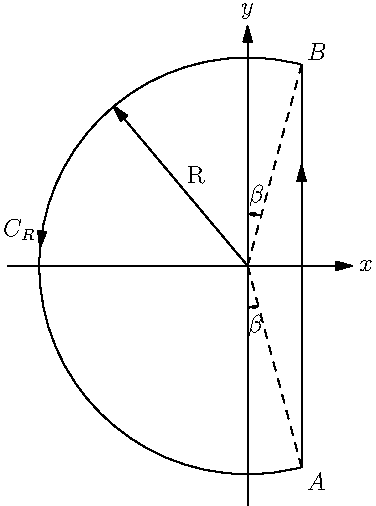
\includegraphics{graphics/contour_simple.pdf}
\end{marginfigure}
%%%%%%%%%%%%%%%%%%%%%%%%%%%%%%%%%%%%

\[
	\oint = \int_{AB} + \int_{C_R}.
\]
Now for $z=R e^{i\theta}$ on contour $C_R$,
$\frac{\pi}{2}-\beta<\theta<\frac{3}{2}\pi+\beta$. Since $|a|<b$, we have
\[
	\lim_{R\to\infty} \max_z \left| \frac{\sinh(\sqrt{z} a)}{\sinh (\sqrt{z} b)}
	\right|
	= \lim_{R\to\infty} \max_{\theta} e^{\sqrt{R} (|a|-b) |\cos\frac{\theta}{2}|}
	=0,
\]
thus by Jordan's Lemma (Corollary \ref{C:jordan}) we have $\int_{C_R}=0$.

Hence
\begin{align*}
	f(t)  
	&= \frac{1}{2\pi i}   
      \int_{c-i\infty}^{c+i\infty} e^{p t} F(p)\, dp  \\
	&= \frac{1}{2\pi i} \oint e^{z t} F(z)\, dz \\
	&= \sum_{n=1}^{\infty} 
	  Res\left[ \frac{e^{tz} \sinh (\sqrt{z} a)}{\sinh (\sqrt{z} b)}; z_n
		\right] \\
	&= \sum_{n=1}^{\infty} 
	  (-)^{n+1} \left( \frac{2n\pi}{b^2} \right) e^{-\frac{n^2\pi^2}{b^2} t} 
	  \sin(\frac{n\pi a}{b}).
\end{align*}
i.e.
\footnote{Doetsch, Introduction to the Theory and Application of the Laplace
Transformation, \#60, p.321; Spiegel, Schaum's Outline of Theory and Problems of
Laplace Transforms, Appendix B.124, p.252, note the missing of a negative sign.}
\begin{equation} \label{E:ilt_sinh_1A}
  f(t)
	= L_p^{-1}\left[ \frac{\sinh (\sqrt{p} a)}{\sinh (\sqrt{p} b)} \right]
	= \sum_{n=1}^{\infty} 
	  (-)^{n+1} \left( \frac{2n\pi}{b^2} \right) e^{-\frac{n^2\pi^2}{b^2} t} 
	  \sin(\frac{n\pi a}{b}).
\end{equation}

An alternative approach is the following. Observe that
\begin{align*}
	F(p) 
	&= \frac{\sinh (\sqrt{p} a)}{\sinh (\sqrt{p} b)}  
	 = \frac{e^{(a-b)\sqrt{p}} - e^{-(a+b)\sqrt{p}}}{1- e^{-2b\sqrt{p}}} \\
	&= (e^{(a-b)\sqrt{p}} - e^{-(a+b)\sqrt{p}}) 
	   \sum_{n=0}^{\infty} e^{-2nb\sqrt{p}} \\
  &= \sum_{n=0}^{\infty} 
		 \left( e^{-(-a+b+2nb)\sqrt{p}} - e^{-(a+b+2nb)\sqrt{p}} \right)
\end{align*}
Using Eq. \ref{E:ilt_1a} we get
\begin{align*}
	f(t) 
	&= L_p^{-1} [F(p)]  \\
  &= \sum_{n=0}^{\infty} 
	   \left( L_p^{-1}[ e^{-(-a+b+2nb)\sqrt{p}} ] 
	        - L_p^{-1}[ e^{-( a+b+2nb)\sqrt{p}} ] \right) \\
	&= \frac{1}{2\sqrt{\pi} t^{{3/2}} }
 		 \sum_{n=0}^{\infty} 
		 \left(
			 (-a+b+2nb) e^{-(-a+b+2nb)^2/4t} - (a+b+2nb) e^{-(a+b+2nb)^2/4t}
		 \right)  \\
  &= \frac{1}{2\sqrt{\pi} t^{{3/2}} }
 		 \sum_{n=-\infty}^{\infty}  (-a+b+2nb) e^{-(-a+b+2nb)^2/4t},
\end{align*}
i.e.,
\footnote{Doetsch, Introduction to the Theory and Application of the Laplace
Transformation, \#60, p.321 and p.200; cf. Borodin and Salemin, Handbook of 
Brownian Motions, 2ed, Appendix 2.11, p.641, defintion of $ss_y$.}
\begin{equation} \label{E:ilt_sinh_1B}
	L_p^{-1}\left[ \frac{\sinh (\sqrt{p} a)}{\sinh (\sqrt{p} b)} \right]
  = \frac{1}{2\sqrt{\pi} t^{{3/2}} }
 		\sum_{n=-\infty}^{\infty}  (-a+b+2nb) e^{-(-a+b+2nb)^2/4t}.
\end{equation}

We now verifty that Eq. \ref{E:ilt_sinh_1B} is equivalent to Eq.
\ref{E:ilt_sinh_1A}. 
Let
\[
  S_2 = \frac{1}{2\sqrt{\pi} t^{{3/2}} }
 		    \sum_{n=-\infty}^{\infty}  (-a+b+2nb) e^{-(-a+b+2nb)^2/4t},
\]
also let $y=\frac{a}{2b}$, we have
\[
	S_2 = \frac{b}{\sqrt{\pi} t^{3/2}}
	\sum_{n=-\infty}^{\infty}  (-y+\frac{1}{2}+n) e^{-(-y+\frac{1}{2}+n)^2 b^2/t},
\]
Now apply the Poisson summation formula, 
\footnote{Borwein and Borwein, Pi and the AGM, Theorem 2.2, p.37; Apostol,
Introduction to Mathematical Analysis, 2ed, pp.332-333.}
we get
\[
	S_2 
	= \sum_{n=-\infty}^{\infty} e^{2\pi i n y}
    \int_{-\infty}^{\infty} e^{-2\pi i n y}
		  \left( \frac{b}{\sqrt{\pi} t^{3/2}} \right)
      (-y+\frac{1}{2}+n) e^{-(-y+\frac{1}{2}+n)^2 b^2/t} \, dy.
\]
We first calculate the following integral
\begin{align*}
	I 
	&= \int_{-\infty}^{\infty} e^{-2\pi i n y}
      (-y+\frac{1}{2}+n) e^{-(-y+\frac{1}{2}+n)^2 b^2/t} \, dy \\
  &= \int_{-\infty}^{\infty} e^{-2\pi i n (x+\frac{1}{2} + n) }
			(-x) e^{-x^2 b^2/t} \, dx       \qquad (x=y-\frac{1}{2}-n) \\
	&= (-)^{n+1} \int_{-\infty}^{\infty} e^{-2\pi i n x} x e^{-x^2 b^2/t} \, dx \\
	&= (-)^n i \int_{-\infty}^{\infty} x \sin (2\pi n x) e^{-x^2 b^2/t} \, dx \\
	&= (-)^n i \frac{t}{b^2} \int_{-\infty}^{\infty} z 
			\sin \left( \frac{2\pi n \sqrt{t}}{b} z \right) e^{-z^2} \, dz,
			\qquad (z=\frac{x b}{\sqrt{t}}),
\end{align*}
using Eq. \ref{E:int2_2} we get
\[
	I = (-)^n i \frac{(\pi t)^{3/2}}{b^3} n e^{-\frac{n^2 \pi^2 t}{b^2}},
\]
hence
\begin{align*}
	S_2
	&= \sum_{n=-\infty}^{\infty} e^{2\pi i n y} \frac{b}{\sqrt{\pi}t^{3/2}}
	   \left( (-)^n i \frac{(\pi t)^{3/2}}{b^3} n e^{-\frac{n^2 \pi^2 t}{b^2}}
		 \right)  \\
  &= \sum_{n=-\infty}^{\infty} i e^{2\pi i n y} (-)^n \frac{n\pi}{b^2}
	       e^{-\frac{n^2 \pi^2 t}{b^2}}   \\
  &= \sum_{n=1}^{\infty} (-)^{n+1} \frac{2n\pi}{b^2} \sin(\frac{n\pi a}{b})
	     e^{-\frac{n^2 \pi^2 t}{b^2}}.
\end{align*}

For convenience we define the following theta function:
\footnote{Borodin and Salemin, Handbook of Brownian Motions, 2ed, Appendix 2.11, 
p.641, defintion of $ss_y$.}
\begin{align} \label{E:theta_ss}
	ss_t(a,b)
	&= L_p^{-1}\left[ \frac{\sinh (\sqrt{2p} a)}{\sinh (\sqrt{2p} b)} \right] 
	  \notag \\
	&= \frac{1}{\sqrt{2\pi} t^{{3/2}} }
 		 \sum_{n=-\infty}^{\infty}  (-a+b+2nb) e^{-(-a+b+2nb)^2/2t} \notag \\
  &= \sum_{n=1}^{\infty} (-)^{n+1} \frac{n\pi}{b^2} \sin(\frac{n\pi a}{b})
	     e^{-\frac{n^2 \pi^2 t}{2 b^2}},   
\end{align}
these two representations come from a straight-forward application of Eq. 
\ref{E:ilt_lin} on Eqs. \ref{E:ilt_sinh_1A} and \ref{E:ilt_sinh_1B}.

%%%%%%%%%%%%%%%%%%%%%%%%%%%%%%%%%%%%%%%%%%%%%%%%%%%%%%%%%%%%%%%%%%%%%%%%%%
\section{$L_p^{-1}[ \frac{\sinh (\sqrt{p} a)}{\sinh (\sqrt{p} b)} 
          \frac{e^{-c\sqrt{p}}}{\sqrt{p}} ], |a|<b, c>0$ }
Similar to the approach used in the previous section, we have
\[
	F[p] = \frac{\sinh (\sqrt{p} a)}{\sinh (\sqrt{p} b)} 
         \frac{e^{-c\sqrt{p}}}{\sqrt{p}} 
				 = \sum_{n=0}^{\infty} 
				 \left(
					 \frac{e^{-(-a+b+c+2nb)\sqrt{p}}}{\sqrt{p}}
					 -\frac{e^{-(a+b+c+2nb)\sqrt{p}}}{\sqrt{p}}
				 \right).
\]
Using Eq. \ref{E:ilt2} we get
\begin{align*}
	f(t)
	&= L_p^{-1}[F(p)]   \\
	&= \sum_{n=0}^{\infty} 
	   \left(
			  L_p^{-1} \left[ \frac{e^{-(-a+b+c+2nb)\sqrt{p}}}{\sqrt{p}} \right]
				-L_p^{-1} \left[ \frac{e^{-(a+b+c+2nb)\sqrt{p}}}{\sqrt{p}} \right]
		 \right) \\
	&= \sum_{n=0}^{\infty} 
	   \left(
			 \frac{ e^{-(-a+b+c+2nb)^2/4t} }{\sqrt{\pi t}}
			 - \frac{ e^{-(a+b+c+2nb)^2/4t} }{\sqrt{\pi t}}
		 \right), 
\end{align*}
i.e.
\begin{equation}
  L_p^{-1}\left[ \frac{\sinh (\sqrt{p} a)}{\sinh (\sqrt{p} b)} 
				         \frac{e^{-c\sqrt{z}}}{\sqrt{z}} \right]
	= \sum_{n=0}^{\infty} 
	   \left(
			 \frac{ e^{-(-a+b+c+2nb)^2/4t} }{\sqrt{\pi t}}
			 - \frac{ e^{-(a+b+c+2nb)^2/4t} }{\sqrt{\pi t}}
		 \right).
\end{equation}

Alternatively we can calculate the inverse Laplace transform using Bromwich 
integral:
\[
  f(t)= L_p^{-1}\left[ \frac{\sinh (\sqrt{p} a)}{\sinh (\sqrt{p} b)} 
				               \frac{e^{-c\sqrt{z}}}{\sqrt{z}} \right]
	    = \frac{1}{2\pi i} 
			  \int_{c-i\infty}^{c+\infty} 
		      e^{zt} \frac{\sinh (\sqrt{z} a)}{\sinh (\sqrt{z} b)} 
				  \frac{e^{-c\sqrt{z}}}{\sqrt{z}} 
				dz.
\]
Note that for function
\[
	F(z)= \frac{1}{2\pi i} e^{zt} \frac{\sinh (\sqrt{z} a)}{\sinh (\sqrt{z} b)} 
			  \frac{e^{-c\sqrt{z}}}{\sqrt{z}},
\]
$z=0$ is a branch point, and there are simple poles at
\[
	z_n=-\frac{n^2 \pi^2}{b^2}, n=1,2,3,\cdots,
\]
hence we select a contour around the branch cut from $z=-\infty$ to $z=0$ (thus
remain on the principal branch), and since all the poles are on the branch cut, 
we use semicircles around them. And we have

%%%%%%%%%%%%%%%%%%%%%%%%%%%%%%%%%%%%
\begin{marginfigure} 
  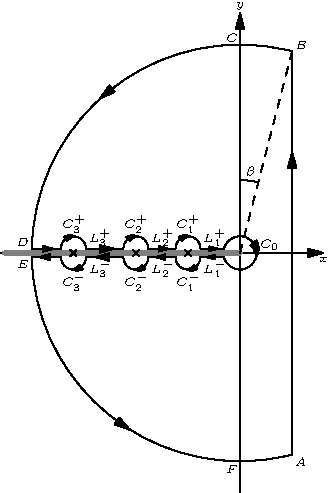
\includegraphics{graphics/contour_sinh.pdf}
	\caption{Contour with a branch cut from $z=-\infty$ to $z=0$ and semicircles
		around simple pole at $z_n=-\frac{n^2 \pi^2}{b^2}, n=1,2,3,\cdots$.}
\end{marginfigure}
%%%%%%%%%%%%%%%%%%%%%%%%%%%%%%%%%%%%

\[
	\oint F(z) dz 
	= \int_{AB} + \int_{BCD} + \int_{EFA} + \int_{C_0} 
	+ \sum_{n=1}^{\infty} 
	  \left( 
			\int_{C_n^+} + \int_{C_n^-} + \int_{L_n^+} + \int_{L_n^-} 
		\right)
 =0.
\]
Since the contour does not include any poles, using the residue theorem on the
principal branch $\sqrt{z}$ we get $\oint =0$. Now on contour $BCD$, 
$z=R e^{i\theta}$, $\frac{\pi}{2}-\beta <\theta <\pi$; while on contour $EFA$, 
$z=R e^{i\theta}$, $-\pi <\theta < -\frac{\pi}{2}+\beta$. Now on $BCD$ and
$EFA$, since $|a|<b$ and $c>0$, we have
\[
	\lim_{R\to\infty} \max_z 
	\left| 
	  \frac{\sinh(\sqrt{z} a)}{\sinh (\sqrt{z} b)} \frac{e^{-c\sqrt{z}}}{\sqrt{z}}
	\right|
	= \lim_{R\to\infty} \max_{\theta} 
	\frac{ e^{\sqrt{R} (|a|-b-c) \cos\frac{\theta}{2}} }
	     { \sqrt{R}\cos\frac{\theta}{2} }
	=0,
\]
thus by Jordan's Lemma (Corollary \ref{C:jordan}) we have 
\[
	\int_{BCD}=\int_{EFA}=0.
\]

And on the small circle $C_0$ we have
\[
	\int_{C_0} = \frac{1}{2\pi i} 
	  \lim_{\epsilon\to 0} \int_{\pi}^{-\pi} e^{t\epsilon e^{i\theta}}
		\frac{a\sqrt{\epsilon}e^{i\theta/2}}{b\sqrt{\epsilon}e^{i\theta/2}}
		\frac{e^{-c\sqrt{\epsilon}e^{i\theta/2}}}{\sqrt{\epsilon} e^{i\theta/2}}
		\epsilon e^{i\theta} i d\theta
	=0.
\]

On contour $C_n^+$, $z=z_n+\epsilon e^{i\theta}, 0<\theta<\pi$, thus
\[
	\sqrt{z}=\sqrt{z_n}+\frac{\epsilon e^{i\theta}}{2\sqrt{z_n}} + o(\epsilon^2),
\]
and
\begin{align*}
	\int_{C_n^+}
	&= \frac{1}{2\pi i} \lim_{\epsilon\to 0} \int_{\pi}^0 \epsilon e^{i\theta} i d\theta
	  \frac{e^{tz_n} \sinh(a\sqrt{z_n}) e^{-c\sqrt{z_n}}}
		{(-)^n \epsilon e^{i\theta} b/2}  \\
		&= \frac{(-)^{n+1}}{b} e^{tz_n} \sinh(a\sqrt{z_n}) e^{-c\sqrt{z_n}},
\end{align*}
while on contour $C_n^-$, $z=z_n e^{2\pi i}+\epsilon e^{i\theta}, \pi<\theta<2\pi$, 
thus
\[
	\sqrt{z}=-\sqrt{z_n}-\frac{\epsilon e^{i\theta}}{2\sqrt{z_n}} + o(\epsilon^2),
\]
and
\begin{align*}
	\int_{C_n^-}
	&= \frac{1}{2\pi i} \lim_{\epsilon\to 0} \int_{2\pi}^{\pi} \epsilon e^{i\theta} i d\theta
	  \frac{e^{tz_n} \sinh(-a\sqrt{z_n}) e^{c\sqrt{z_n}}}
		{(-)^{n} \epsilon e^{i\theta} b/2}  \\
		&= \frac{(-)^{n+1}}{b} e^{tz_n} \sinh(-a\sqrt{z_n}) e^{c\sqrt{z_n}} \\
		&= \frac{(-)^{n}}{b} e^{tz_n} \sinh(a\sqrt{z_n}) e^{c\sqrt{z_n}},
\end{align*}
hence
\begin{align*}
	\int_{C_n^+} + \int_{C_n^-}
	&= \frac{(-)^{n}}{b} e^{t z_n} \sinh(a\sqrt{z_n}) 
	   (e^{c\sqrt{z_n}} - e^{-c\sqrt{z_n}}) \\
		 &= (-)^n \frac{2}{b} e^{-\frac{n^2 \pi^2 t}{b^2}} \sin(\frac{n\pi a}{b}) 
        \sin(\frac{n\pi c}{b}).
\end{align*}

           % Laplace transform and inverse Laplace transform
\chapter{Special Functions}

%%%%%%%%%%%%%%%%%%%%%%%%%%%%%%%%%%%%%%%%%%%%%%%%%%%%%%%%%%%%
\section{Gamma Function}

%%%%%%%%%%%%%%%%%%%%%%%%%%%%
\begin{definition} \label{D:gamma}
The gamma function is defined by 
\begin{equation}
  \Gamma(z) = \int_0^{\infty} t^{z-1} e^{-t} dt.
\end{equation}
\end{definition}

%%%%%%%%%%%%%%%%%%%%%%%%%%%%
\begin{proposition} \label{P:gamma_pp}
The gamma function $\Gamma(z)$ has the following properties:
\begin{enumerate}
  \item[(1)] $\Gamma(z+1) = z\Gamma(z)$.
  \item[(2)] Euler's reflection formula:
    \begin{equation}
      \Gamma(1-z) \Gamma(z) = \frac{\pi}{\sin(\pi z)}.
    \end{equation}
\end{enumerate}
\end{proposition}
\begin{proof}
(1) is trivial using integral by parts.

To verify (2), 
\footnote{Adapted from Andrews et.al., Special Functions, Theorem 1.2.1,
    pp.9-10.}
note that we only need to verify the case with $0<x<1$ because
\[
  \Gamma(x+1)\Gamma(-x) = \Gamma(x) x \frac{\Gamma(1-x)}{-x} 
    =-\frac{\pi}{\sin(\pi x)} =\frac{\pi}{\sin(\pi (x+1))}.
\]
   
For the case with $0<x<1$, first observe that 
\[
  \Gamma(x) \Gamma(1-x) 
    = \int_0^{\infty} ds \int_0^{\infty} dt \,
        t^{x-1} s^{-x} e^{-(t+s)}.
\]
We define two new variables $u=s+t$ and $v=t/s$, hence
\[
  s=\frac{u}{1+v}, \qquad t=\frac{uv}{1+v},
\]
and the Jacobian determinant is
\[
  \left| 
    \begin{array}{cc}
      \frac{\partial u}{\partial t} & \frac{\partial u}{\partial s}  \\
      \frac{\partial v}{\partial t} & \frac{\partial v}{\partial s}  \\
    \end{array}
  \right|
  = \left| 
      \begin{array}{cc}
        1 & 1\\
        \frac{1}{s} & -\frac{t}{s^2}  \\
      \end{array}
    \right|
  =  -\frac{u}{s^2},
\]
hence
\[
  du\, dv = -\frac{u}{s^2} ds \, dt
          = -\frac{(1+v)^2}{u} ds \, dt,
\]
and 
\[
  \Gamma(x) \Gamma(1-x) 
    = - \int_0^{\infty} dv \int_0^{\infty} du 
        \frac{v^{x-1}}{1+v} e^{-u}
    = \int_0^{\infty} \frac{v^{x-1}}{1+v} dv.
\]
To evaluate this (real) integral we use the contour integral
\footnote{Note the sign change in the denominator, this is caused by our contour
    choice.}
\[
   \int_C \frac{z^{x-1}}{1-z} dz
\]
with the following contour where the negative $x$-axis is the branch cut.

%%%%%%%%%%%%%%%%%%%%%%%%%%%%%%%%%%%%
\begin{marginfigure} \label{F:cont_gamma}
  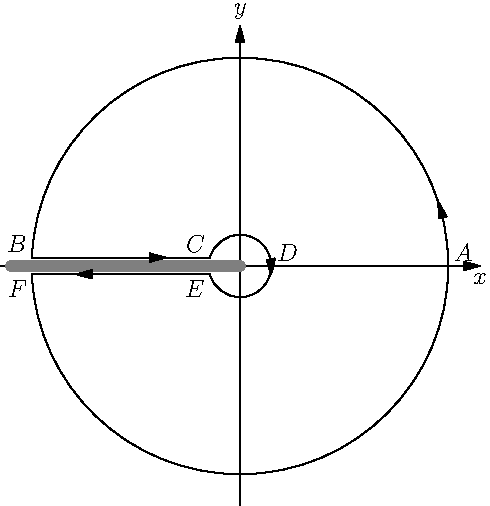
\includegraphics{graphics/contour_euler.pdf}
	\caption{Contour with a branch cut on the negative $x$-axis.}
\end{marginfigure}
%%%%%%%%%%%%%%%%%%%%%%%%%%%%%%%%%%%%

Using the Cauchy's theorem, we have
\[
   \int_C \frac{z^{x-1}}{1-z} dz = 2\pi i \, Res(z=1) = -2\pi i.
\]
Note that
\[
  \oint = \int_{FAB} + \int_{BC} + \int_{CDE} + \int_{EF},
\]
and it is easy to see that $\int_{FAB}=0$ from Jordan's lemma \ref{L:jordan}, 
and $\int_{CDE}=0$ because
\[
  \lim_{\epsilon\to 0} \left| \int_{CDE} \frac{z^{x-1}}{1-z} dz \right|
    \le \lim_{\epsilon\to 0} \int_{\pi}^{-\pi} 
      \frac{\epsilon^{x}}{|1-\epsilon e^{i\theta}|} d\theta 
    = 0.
\]
For line $BC$, let $z=w e^{i\pi}$, we get
\[
  \int_{BC} = \int_{\infty}^0 \frac{(we^{i\pi})^{x-1}}{1-we^{i\pi}} d(we^{i\pi})
     = -e^{i\pi x} \int_0^{\infty} \frac{w^{x-1}}{1+w} dw.
\]
For line $EF$, let $z=w e^{-i\pi}$, we get
\[
  \int_{EF} = \int_{\infty}^0 \frac{(we^{-i\pi})^{x-1}}{1-we^{-i\pi}} d(we^{-i\pi})
     = e^{-i\pi x} \int_0^{\infty} \frac{w^{x-1}}{1+w} dw.
\]
Hence we have
\[
  \int_{BC}+\int_{EF} 
    = (e^{-i\pi x}-e^{i\pi x}) \int_0^{\infty} \frac{w^{x-1}}{1+w} dw
    =-2\pi i,
\]
i.e.
\[
   \int_0^{\infty} \frac{w^{x-1}}{1+w} dw = \frac{\pi}{\sin(\pi x)},
\]
thus
\[
  \Gamma(1-x) \Gamma(x) = \frac{\pi}{\sin(\pi x)}.
 \]
\end{proof}


%%%%%%%%%%%%%%%%%%%%%%%%%%%%%%%%%%%%%%%%%%%%%%%%%%%%%%%%%%%%
\section{Bessel Function}

%%%%%%%%%%%%%%%%%%%%%%%%%%%%
\begin{definition} \label{D:bessel}
The modified Bessle function $J_{\nu}$ is defined by 
\footnote{Watson, A Treatise on the Theory of Bessel Functions, 3.7.(2), p77}
\begin{equation}
  J_{\nu}(z) = \sum_{m=0}^{\infty} \frac{(-)^m}{m! \Gamma(\nu+m+1)}
                \left(\frac{z}{2}\right)^{\nu+2m},
\end{equation}
\end{definition}

%%%%%%%%%%%%%%%%%%%%%%%%%%%%
\begin{definition} \label{D:bessel_mod}
The modified Bessle function $I_{\nu}$ is defined by 
\footnote{Watson, A Treatise on the Theory of Bessel Functions, 3.7.(2), p77}
\begin{equation}
  I_{\nu}(z) = \sum_{m=0}^{\infty} \frac{1}{m! \Gamma(\nu+m+1)}
                \left(\frac{z}{2}\right)^{\nu+2m},
\end{equation}
and $K_{\nu}$ is defined by
\begin{equation}
  K_{\nu}(z)=\frac{\pi}{2\sin{\pi\nu}} (I_{-\nu}(z) - I_{\nu}(z)).
\end{equation}
And $I_{\nu}(z)$ and $K_{\nu}(z)$ are independent solutions of the differential 
equation
\begin{equation}
  z^2 u''(z)+ z u'(z) - (z^2+\nu^2) u(z) = 0.
\end{equation}
\end{definition}

%%%%%%%%%%%%%%%%%%%%%%%%%%%%
\begin{proposition} \label{P:bessel_mod}
We have the following useful properties for the modified Bessel functions:
\begin{enumerate}
  \item[(1)] $K_{-\nu}(z) = K_{\nu}(z)$.
  \item[(2)] $I_{\nu}(z e^{in\pi}) = e^{in\nu\pi} I_{\nu}(z)$, and specifically
             $I_{\nu}(-z)=e^{i\nu\pi}I_{\nu}(z)$, here $n\in Z$.
  \item[(3)] $I_{\nu}(-x) K_{\nu}(-y) -I_{\nu}(x) K_{\nu}(y) =
  \frac{\pi}{2\sin(\pi\nu)} I_{\nu}(x) I_{\nu}(y) (e^{2i\nu\pi}-1)$.
\end{enumerate}
\end{proposition}
      % special functions

\appendix
\chapter{A Useful Calculation} \label{A:useful}

Given a Gaussian random variable $X\sim N(\mu,\sigma^2)$, we have
\begin{equation} \label{E:int_call}
  E[(e^X-K)^+] = 
    e^{\mu+\frac{\sigma^2}{2}} 
      \Phi \left( \frac{\mu-\log{K}}{\sigma}+\sigma \right)
    -K \Phi \left( \frac{\mu-\log{K}}{\sigma} \right),
\end{equation}
and
\begin{equation} \label{E:int_put}
  E[(K-e^X)^+] = 
    K \Phi \left( \frac{\log{K}-\mu}{\sigma} \right)
    - e^{\mu+\frac{\sigma^2}{2}} 
      \Phi \left( \frac{\log{K}-\mu}{\sigma}-\sigma \right),
\end{equation}
where 
\[
  \Phi(x) = \int_{-\infty}^x \frac{e^{-t^2/2}}{\sqrt{2\pi}} dt
\]
is the cumulative Gaussian function.

Note that these satisfy
\[
  E[(e^X-K)^+] - E[(K-e^X)^+] = e^{\mu+\frac{\sigma^2}{2}} - K.
\]

%%%%%%%%%%%%%%%%%%%%%%%%%%%%%%%%%%
\begin{proof}
\begin{align*}
  E[(e^X-K)^+] 
    &= E[ (e^X-K) 1_{e^X>K} ] \notag \\
    &= E[ (e^X-K) 1_{X>\log K} ] \notag \\
    &= \int_{\log K}^{\infty} (e^x-K) 
       \frac{e^{-\frac{(x-\mu)^2}{2\sigma^2}}}{\sigma\sqrt{2\pi}} dx \notag \\
\end{align*}
Let
\[
  y = \frac{\mu -x}{\sigma},
\]
then we have
\begin{align*}
  E[(e^X-K)^+] 
    &= \int_{-\infty}^{\frac{\mu-\log K}{\sigma}} (e^{\mu-\sigma y}-K)
         \frac{e^{-\frac{y^2}{2}}}{\sqrt{2\pi}} dy \notag \\
    &= \int_{-\infty}^{\frac{\mu-\log K}{\sigma}} e^{\mu+\frac{\sigma^2}{2}}
         \frac{e^{-\frac{(y+\sigma)^2}{2}}}{\sqrt{2\pi}} dy 
       - K \int_{-\infty}^{\frac{\mu-\log K}{\sigma}} 
         \frac{e^{-\frac{y^2}{2}}}{\sqrt{2\pi}} dy \notag \\
   &= e^{\mu+\frac{\sigma^2}{2}} 
        \Phi \left( \frac{\mu-\log{K}}{\sigma}+\sigma \right)
      -K \Phi \left( \frac{\mu-\log{K}}{\sigma} \right). \notag \\
\end{align*}

Similarly we have
\begin{align*}
  E[(K-e^X)^+] 
    &= E[ (K-e^X) 1_{e^X<K} ] \notag \\
    &= E[ (K-e^X) 1_{X<\log K} ] \notag \\
    &= \int^{\log K}_{-\infty} (K-e^x) 
       \frac{e^{-\frac{(x-\mu)^2}{2\sigma^2}}}{\sigma\sqrt{2\pi}} dx \notag \\
\end{align*}
Now let
\[
  y = \frac{x- \mu}{\sigma},
\]
then we have
\begin{align*}
  E[(e^X-K)^+] 
    &= \int_{-\infty}^{\frac{\log K-\mu}{\sigma}} (K-e^{\mu+\sigma y})
         \frac{e^{-\frac{y^2}{2}}}{\sqrt{2\pi}} dy \notag \\
    &=  K \int_{-\infty}^{\frac{\log K-\mu}{\sigma}} 
         \frac{e^{-\frac{y^2}{2}}}{\sqrt{2\pi}} dy 
        - \int_{-\infty}^{\frac{\log K-\mu}{\sigma}} e^{\mu+\frac{\sigma^2}{2}}
         \frac{e^{-\frac{(y-\sigma)^2}{2}}}{\sqrt{2\pi}} dy      \notag \\
   &= K \Phi \left( \frac{\log{K}-\mu}{\sigma} \right) 
      - e^{\mu+\frac{\sigma^2}{2}} 
        \Phi \left( \frac{\log{K}-\mu}{\sigma}-\sigma \right)     \notag \\
\end{align*}
\end{proof}
    % an useful integral for option price
\chapter{Levenberg-Marquardt Algorithm} \label{C:levenberg}

Levenberg-Marquardt algorithm is an algorithm for minimizing a function and it
is between the Gauss-Newton algorithm and the method of gradient descent.

\section{Least Square Problem}
Given a set of $m$ observations of pairs of independent and dependent variables
$(x_i,y_i)$, optimize the parameters $\beta$ of the model curve $f(x,\beta)$ so
that the sum of the square of the deviations
\[
  S(\beta) = \sum_{i=1}^m [y_i - f(x_i,\beta)]^2
\]
becomes minimal.

\section{The Algorithm}
The Levenberg-Marquardt algorithm is an iterative procedure. At the beginning
the user has to provide an initial guess of the parameter vector $\beta$. In
each step, the parameter vector $\beta$ is replaced by a new estimate
$\beta+\delta$. To determine $\delta$, the functions $f(x_i,\beta+\delta)$ are
approximated by
\[
  f(x_i,\beta+\delta) \approx f(x_i,\beta) + J_i \delta, 
\]
where
\[
  J_i = \frac{\partial f(x_i,\beta)}{\partial \beta}
\]
is the gradient of $f$ with respect to $\beta$. Hence 
\[
  S(\beta+\delta) \approx \sum_{i=1}^m (y_i - f(x_i,\beta)-J_i\delta)^2
\]
For this to be minimal, the derivative with respect to $\delta$ must be zero,
this yields
\[
  (J^T J) \delta = J^T [y-f(\beta)],
\]
where $J$ is the Jacobian matrix with elements
\[
  J_{ij} = \frac{\partial f(x_i,\beta)}{\partial \beta_j}.
\]
Solving this equation we would get $\delta$. And this is the idea for
Guass-Newton algorithm.

Now Levenberg-Marquardt algorithm introduces a (non-negative damping factor
$\lambda$
\[
  (J^T J + \lambda I) \delta = J^T [y-f(\beta)],
\]
where $I$ is the identity matrix.
The damping factor is adjusted at every iteration. If reduction of $S$ is rapid,
a smaller $\lambda$ can be used bringing it closer to the Gauss-Newton
algorithm; if reduction is slow, a larger $\lambda$ can be used bringing it
closer to gradient descent.

   % Levenberg-Marquardt algorithm


\end{document}

